\documentclass[14pt,fleqn]{extbook} % Default font size and left-justified equations
\usepackage{graphicx}
\usepackage{setspace}
\usepackage{graphicx} % Required for including pictures
\graphicspath{{Pictures/}} % Specifies the directory where pictures are stored

\usepackage{lipsum} % Inserts dummy text

\usepackage{tikz} % Required for drawing custom shapes

\usepackage[english]{babel} % English language/hyphenation

\usepackage{enumitem} % Customize lists
\setlist{nolistsep} % Reduce spacing between bullet points and numbered lists

\usepackage{booktabs} % Required for nicer horizontal rules in tables

\usepackage{xcolor} % Required for specifying colors by name
\definecolor{ocre}{RGB}{243,102,25} % Define the orange color used for highlighting throughout the book

%----------------------------------------------------------------------------------------
%	MARGINS
%----------------------------------------------------------------------------------------

\usepackage{geometry} % Required for adjusting page dimensions and margins

\geometry{
	paper=a4paper, % Paper size, change to letterpaper for US letter size
	top=3cm, % Top margin
	bottom=3cm, % Bottom margin
	left=3cm, % Left margin
	right=3cm, % Right margin
	headheight=14pt, % Header height
	footskip=1.4cm, % Space from the bottom margin to the baseline of the footer
	headsep=10pt, % Space from the top margin to the baseline of the header
	%showframe, % Uncomment to show how the type block is set on the page
}

%----------------------------------------------------------------------------------------
%	FONTS
%----------------------------------------------------------------------------------------

\usepackage{avant} % Use the Avantgarde font for headings
%\usepackage{times} % Use the Times font for headings
\usepackage{mathptmx} % Use the Adobe Times Roman as the default text font together with math symbols from the Sym­bol, Chancery and Com­puter Modern fonts

\usepackage{microtype} % Slightly tweak font spacing for aesthetics
\usepackage[utf8]{inputenc} % Required for including letters with accents
\usepackage[T1]{fontenc} % Use 8-bit encoding that has 256 glyphs

%----------------------------------------------------------------------------------------
%	BIBLIOGRAPHY AND INDEX
%----------------------------------------------------------------------------------------

\usepackage[style=numeric,citestyle=numeric,sorting=nyt,sortcites=true,autopunct=true,babel=hyphen,hyperref=true,abbreviate=false,backref=true,backend=biber]{biblatex}
\addbibresource{bibliography.bib} % BibTeX bibliography file
\defbibheading{bibempty}{}

\usepackage{calc} % For simpler calculation - used for spacing the index letter headings correctly
\usepackage{makeidx} % Required to make an index
\makeindex % Tells LaTeX to create the files required for indexing

%----------------------------------------------------------------------------------------
%	MAIN TABLE OF CONTENTS
%----------------------------------------------------------------------------------------

\usepackage{titletoc} % Required for manipulating the table of contents

\contentsmargin{0cm} % Removes the default margin

% Part text styling (this is mostly taken care of in the PART HEADINGS section of this file)
\titlecontents{part}
	[0cm] % Left indentation
	{\addvspace{20pt}\bfseries} % Spacing and font options for parts
	{}
	{}
	{}

% Chapter text styling
\titlecontents{chapter}
	[1.25cm] % Left indentation
	{\addvspace{12pt}\large\sffamily\bfseries} % Spacing and font options for chapters
	{\color{ocre!60}\contentslabel[\Large\thecontentslabel]{1.25cm}\color{ocre}} % Formatting of numbered sections of this type
	{\color{ocre}} % Formatting of numberless sections of this type
	{\color{ocre!60}\normalsize\;\titlerule*[.5pc]{.}\;\thecontentspage} % Formatting of the filler to the right of the heading and the page number

% Section text styling
\titlecontents{section}
	[1.25cm] % Left indentation
	{\addvspace{3pt}\sffamily\bfseries} % Spacing and font options for sections
	{\contentslabel[\thecontentslabel]{1.25cm}} % Formatting of numbered sections of this type
	{} % Formatting of numberless sections of this type
	{\hfill\color{black}\thecontentspage} % Formatting of the filler to the right of the heading and the page number

% Subsection text styling
\titlecontents{subsection}
	[1.25cm] % Left indentation
	{\addvspace{1pt}\sffamily\small} % Spacing and font options for subsections
	{\contentslabel[\thecontentslabel]{1.25cm}} % Formatting of numbered sections of this type
	{} % Formatting of numberless sections of this type
	{\ \titlerule*[.5pc]{.}\;\thecontentspage} % Formatting of the filler to the right of the heading and the page number

% Figure text styling
\titlecontents{figure}
	[1.25cm] % Left indentation
	{\addvspace{1pt}\sffamily\small} % Spacing and font options for figures
	{\thecontentslabel\hspace*{1em}} % Formatting of numbered sections of this type
	{} % Formatting of numberless sections of this type
	{\ \titlerule*[.5pc]{.}\;\thecontentspage} % Formatting of the filler to the right of the heading and the page number

% Table text styling
\titlecontents{table}
	[1.25cm] % Left indentation
	{\addvspace{1pt}\sffamily\small} % Spacing and font options for tables
	{\thecontentslabel\hspace*{1em}} % Formatting of numbered sections of this type
	{} % Formatting of numberless sections of this type
	{\ \titlerule*[.5pc]{.}\;\thecontentspage} % Formatting of the filler to the right of the heading and the page number

%----------------------------------------------------------------------------------------
%	MINI TABLE OF CONTENTS IN PART HEADS
%----------------------------------------------------------------------------------------

% Chapter text styling
\titlecontents{lchapter}
	[0em] % Left indentation
	{\addvspace{15pt}\large\sffamily\bfseries} % Spacing and font options for chapters
	{\color{ocre}\contentslabel[\Large\thecontentslabel]{1.25cm}\color{ocre}} % Chapter number
	{}  
	{\color{ocre}\normalsize\sffamily\bfseries\;\titlerule*[.5pc]{.}\;\thecontentspage} % Page number

% Section text styling
\titlecontents{lsection}
	[0em] % Left indentation
	{\sffamily\small} % Spacing and font options for sections
	{\contentslabel[\thecontentslabel]{1.25cm}} % Section number
	{}
	{}

% Subsection text styling (note these aren't shown by default, display them by searchings this file for tocdepth and reading the commented text)
\titlecontents{lsubsection}
	[.5em] % Left indentation
	{\sffamily\footnotesize} % Spacing and font options for subsections
	{\contentslabel[\thecontentslabel]{1.25cm}}
	{}
	{}

%----------------------------------------------------------------------------------------
%	HEADERS AND FOOTERS
%----------------------------------------------------------------------------------------

\usepackage{fancyhdr} % Required for header and footer configuration

\pagestyle{fancy} % Enable the custom headers and footers

\renewcommand{\chaptermark}[1]{\markboth{\sffamily\normalsize\bfseries\chaptername\ \thechapter.\ #1}{}} % Styling for the current chapter in the header
\renewcommand{\sectionmark}[1]{\markright{\sffamily\normalsize\thesection\hspace{5pt}#1}{}} % Styling for the current section in the header

\fancyhf{} % Clear default headers and footers
\fancyhead[LE,RO]{\sffamily\normalsize\thepage} % Styling for the page number in the header
\fancyhead[LO]{\rightmark} % Print the nearest section name on the left side of odd pages
\fancyhead[RE]{\leftmark} % Print the current chapter name on the right side of even pages
%\fancyfoot[C]{\thepage} % Uncomment to include a footer

\renewcommand{\headrulewidth}{0.5pt} % Thickness of the rule under the header

\fancypagestyle{plain}{% Style for when a plain pagestyle is specified
	\fancyhead{}\renewcommand{\headrulewidth}{0pt}%
}

% Removes the header from odd empty pages at the end of chapters
\makeatletter
\renewcommand{\cleardoublepage}{
\clearpage\ifodd\c@page\else
\hbox{}
\vspace*{\fill}
\thispagestyle{empty}
\newpage
\fi}

%----------------------------------------------------------------------------------------
%	THEOREM STYLES
%----------------------------------------------------------------------------------------

\usepackage{amsmath,amsfonts,amssymb,amsthm} % For math equations, theorems, symbols, etc

\newcommand{\intoo}[2]{\mathopen{]}#1\,;#2\mathclose{[}}
\newcommand{\ud}{\mathop{\mathrm{{}d}}\mathopen{}}
\newcommand{\intff}[2]{\mathopen{[}#1\,;#2\mathclose{]}}
\renewcommand{\qedsymbol}{$\blacksquare$}
\newtheorem{notation}{Notation}[chapter]

% Boxed/framed environments
\newtheoremstyle{ocrenumbox}% Theorem style name
{0pt}% Space above
{0pt}% Space below
{\normalfont}% Body font
{}% Indent amount
{\small\bf\sffamily\color{ocre}}% Theorem head font
{\;}% Punctuation after theorem head
{0.25em}% Space after theorem head
{\small\sffamily\color{ocre}\thmname{#1}\nobreakspace\thmnumber{\@ifnotempty{#1}{}\@upn{#2}}% Theorem text (e.g. Theorem 2.1)
\thmnote{\nobreakspace\the\thm@notefont\sffamily\bfseries\color{black}---\nobreakspace#3.}} % Optional theorem note

\newtheoremstyle{blacknumex}% Theorem style name
{5pt}% Space above
{5pt}% Space below
{\normalfont}% Body font
{} % Indent amount
{\small\bf\sffamily}% Theorem head font
{\;}% Punctuation after theorem head
{0.25em}% Space after theorem head
{\small\sffamily{\tiny\ensuremath{\blacksquare}}\nobreakspace\thmname{#1}\nobreakspace\thmnumber{\@ifnotempty{#1}{}\@upn{#2}}% Theorem text (e.g. Theorem 2.1)
\thmnote{\nobreakspace\the\thm@notefont\sffamily\bfseries---\nobreakspace#3.}}% Optional theorem note

\newtheoremstyle{blacknumbox} % Theorem style name
{0pt}% Space above
{0pt}% Space below
{\normalfont}% Body font
{}% Indent amount
{\small\bf\sffamily}% Theorem head font
{\;}% Punctuation after theorem head
{0.25em}% Space after theorem head
{\small\sffamily\thmname{#1}\nobreakspace\thmnumber{\@ifnotempty{#1}{}\@upn{#2}}% Theorem text (e.g. Theorem 2.1)
\thmnote{\nobreakspace\the\thm@notefont\sffamily\bfseries---\nobreakspace#3.}}% Optional theorem note

% Non-boxed/non-framed environments
\newtheoremstyle{ocrenum}% Theorem style name
{5pt}% Space above
{5pt}% Space below
{\normalfont}% Body font
{}% Indent amount
{\small\bf\sffamily\color{ocre}}% Theorem head font
{\;}% Punctuation after theorem head
{0.25em}% Space after theorem head
{\small\sffamily\color{ocre}\thmname{#1}\nobreakspace\thmnumber{\@ifnotempty{#1}{}\@upn{#2}}% Theorem text (e.g. Theorem 2.1)
\thmnote{\nobreakspace\the\thm@notefont\sffamily\bfseries\color{black}---\nobreakspace#3.}} % Optional theorem note
\makeatother

% Defines the theorem text style for each type of theorem to one of the three styles above
\newcounter{dummy} 
\numberwithin{dummy}{section}
\theoremstyle{ocrenumbox}
\newtheorem{theoremeT}[dummy]{Theorem}
\newtheorem{problem}{Problem}[chapter]
\newtheorem{exerciseT}{Exercise}[chapter]
\theoremstyle{blacknumex}
\newtheorem{exampleT}{Example}[chapter]
\theoremstyle{blacknumbox}
\newtheorem{vocabulary}{Vocabulary}[chapter]
\newtheorem{definitionT}{Definition}[section]
\newtheorem{corollaryT}[dummy]{Corollary}
\theoremstyle{ocrenum}
\newtheorem{proposition}[dummy]{Proposition}

%----------------------------------------------------------------------------------------
%	DEFINITION OF COLORED BOXES
%----------------------------------------------------------------------------------------

\RequirePackage[framemethod=default]{mdframed} % Required for creating the theorem, definition, exercise and corollary boxes

% Theorem box
\newmdenv[skipabove=7pt,
skipbelow=7pt,
backgroundcolor=black!5,
linecolor=ocre,
innerleftmargin=5pt,
innerrightmargin=5pt,
innertopmargin=5pt,
leftmargin=0cm,
rightmargin=0cm,
innerbottommargin=5pt]{tBox}

% Exercise box	  
\newmdenv[skipabove=7pt,
skipbelow=7pt,
rightline=false,
leftline=true,
topline=false,
bottomline=false,
backgroundcolor=ocre!10,
linecolor=ocre,
innerleftmargin=5pt,
innerrightmargin=5pt,
innertopmargin=5pt,
innerbottommargin=5pt,
leftmargin=0cm,
rightmargin=0cm,
linewidth=4pt]{eBox}	

% Definition box
\newmdenv[skipabove=7pt,
skipbelow=7pt,
rightline=false,
leftline=true,
topline=false,
bottomline=false,
linecolor=ocre,
innerleftmargin=5pt,
innerrightmargin=5pt,
innertopmargin=0pt,
leftmargin=0cm,
rightmargin=0cm,
linewidth=4pt,
innerbottommargin=0pt]{dBox}	

% Corollary box
\newmdenv[skipabove=7pt,
skipbelow=7pt,
rightline=false,
leftline=true,
topline=false,
bottomline=false,
linecolor=gray,
backgroundcolor=black!5,
innerleftmargin=5pt,
innerrightmargin=5pt,
innertopmargin=5pt,
leftmargin=0cm,
rightmargin=0cm,
linewidth=4pt,
innerbottommargin=5pt]{cBox}

% Creates an environment for each type of theorem and assigns it a theorem text style from the "Theorem Styles" section above and a colored box from above
\newenvironment{theorem}{\begin{tBox}\begin{theoremeT}}{\end{theoremeT}\end{tBox}}
\newenvironment{exercise}{\begin{eBox}\begin{exerciseT}}{\hfill{\color{ocre}\tiny\ensuremath{\blacksquare}}\end{exerciseT}\end{eBox}}				  
\newenvironment{definition}{\begin{dBox}\begin{definitionT}}{\end{definitionT}\end{dBox}}	
\newenvironment{example}{\begin{exampleT}}{\hfill{\tiny\ensuremath{\blacksquare}}\end{exampleT}}		
\newenvironment{corollary}{\begin{cBox}\begin{corollaryT}}{\end{corollaryT}\end{cBox}}	

%----------------------------------------------------------------------------------------
%	REMARK ENVIRONMENT
%----------------------------------------------------------------------------------------

\newenvironment{remark}{\par\vspace{10pt}\small % Vertical white space above the remark and smaller font size
\begin{list}{}{
\leftmargin=35pt % Indentation on the left
\rightmargin=25pt}\item\ignorespaces % Indentation on the right
\makebox[-2.5pt]{\begin{tikzpicture}[overlay]
\node[draw=ocre!60,line width=1pt,circle,fill=ocre!25,font=\sffamily\bfseries,inner sep=2pt,outer sep=0pt] at (-15pt,0pt){\textcolor{ocre}{R}};\end{tikzpicture}} % Orange R in a circle
\advance\baselineskip -1pt}{\end{list}\vskip5pt} % Tighter line spacing and white space after remark

%----------------------------------------------------------------------------------------
%	SECTION NUMBERING IN THE MARGIN
%----------------------------------------------------------------------------------------

\makeatletter
\renewcommand{\@seccntformat}[1]{\llap{\textcolor{ocre}{\csname the#1\endcsname}\hspace{1em}}}                    
\renewcommand{\section}{\@startsection{section}{1}{\z@}
{-4ex \@plus -1ex \@minus -.4ex}
{1ex \@plus.2ex }
{\normalfont\large\sffamily\bfseries}}
\renewcommand{\subsection}{\@startsection {subsection}{2}{\z@}
{-3ex \@plus -0.1ex \@minus -.4ex}
{0.5ex \@plus.2ex }
{\normalfont\sffamily\bfseries}}
\renewcommand{\subsubsection}{\@startsection {subsubsection}{3}{\z@}
{-2ex \@plus -0.1ex \@minus -.2ex}
{.2ex \@plus.2ex }
{\normalfont\small\sffamily\bfseries}}                        
\renewcommand\paragraph{\@startsection{paragraph}{4}{\z@}
{-2ex \@plus-.2ex \@minus .2ex}
{.1ex}
{\normalfont\small\sffamily\bfseries}}

%----------------------------------------------------------------------------------------
%	PART HEADINGS
%----------------------------------------------------------------------------------------

% Numbered part in the table of contents
\newcommand{\@mypartnumtocformat}[2]{%
	\setlength\fboxsep{0pt}%
	\noindent\colorbox{ocre!20}{\strut\parbox[c][.7cm]{\ecart}{\color{ocre!70}\Large\sffamily\bfseries\centering#1}}\hskip\esp\colorbox{ocre!40}{\strut\parbox[c][.7cm]{\linewidth-\ecart-\esp}{\Large\sffamily\centering#2}}%
}

% Unnumbered part in the table of contents
\newcommand{\@myparttocformat}[1]{%
	\setlength\fboxsep{0pt}%
	\noindent\colorbox{ocre!40}{\strut\parbox[c][.7cm]{\linewidth}{\Large\sffamily\centering#1}}%
}

\newlength\esp
\setlength\esp{4pt}
\newlength\ecart
\setlength\ecart{1.2cm-\esp}
\newcommand{\thepartimage}{}%
\newcommand{\partimage}[1]{\renewcommand{\thepartimage}{#1}}%
\def\@part[#1]#2{%
\ifnum \c@secnumdepth >-2\relax%
\refstepcounter{part}%
\addcontentsline{toc}{part}{\texorpdfstring{\protect\@mypartnumtocformat{\thepart}{#1}}{\partname~\thepart\ ---\ #1}}
\else%
\addcontentsline{toc}{part}{\texorpdfstring{\protect\@myparttocformat{#1}}{#1}}%
\fi%
\startcontents%
\markboth{}{}%
{\thispagestyle{empty}%
\begin{tikzpicture}[remember picture,overlay]%
\node at (current page.north west){\begin{tikzpicture}[remember picture,overlay]%	
\fill[ocre!20](0cm,0cm) rectangle (\paperwidth,-\paperheight);
\node[anchor=north] at (4cm,-3.25cm){\color{ocre!40}\fontsize{220}{100}\sffamily\bfseries\thepart}; 
\node[anchor=south east] at (\paperwidth-1cm,-\paperheight+1cm){\parbox[t][][t]{8.5cm}{
\printcontents{l}{0}{\setcounter{tocdepth}{1}}% The depth to which the Part mini table of contents displays headings; 0 for chapters only, 1 for chapters and sections and 2 for chapters, sections and subsections
}};
\node[anchor=north east] at (\paperwidth-1.5cm,-3.25cm){\parbox[t][][t]{15cm}{\strut\raggedleft\color{white}\fontsize{30}{30}\sffamily\bfseries#2}};
\end{tikzpicture}};
\end{tikzpicture}}%
\@endpart}
\def\@spart#1{%
\startcontents%
\phantomsection
{\thispagestyle{empty}%
\begin{tikzpicture}[remember picture,overlay]%
\node at (current page.north west){\begin{tikzpicture}[remember picture,overlay]%	
\fill[ocre!20](0cm,0cm) rectangle (\paperwidth,-\paperheight);
\node[anchor=north east] at (\paperwidth-1.5cm,-3.25cm){\parbox[t][][t]{15cm}{\strut\raggedleft\color{white}\fontsize{30}{30}\sffamily\bfseries#1}};
\end{tikzpicture}};
\end{tikzpicture}}
\addcontentsline{toc}{part}{\texorpdfstring{%
\setlength\fboxsep{0pt}%
\noindent\protect\colorbox{ocre!40}{\strut\protect\parbox[c][.7cm]{\linewidth}{\Large\sffamily\protect\centering #1\quad\mbox{}}}}{#1}}%
\@endpart}
\def\@endpart{\vfil\newpage
\if@twoside
\if@openright
\null
\thispagestyle{empty}%
\newpage
\fi
\fi
\if@tempswa
\twocolumn
\fi}

%----------------------------------------------------------------------------------------
%	CHAPTER HEADINGS
%----------------------------------------------------------------------------------------

% A switch to conditionally include a picture, implemented by Christian Hupfer
\newif\ifusechapterimage
\usechapterimagetrue
\newcommand{\thechapterimage}{}%
\newcommand{\chapterimage}[1]{\ifusechapterimage\renewcommand{\thechapterimage}{#1}\fi}%
\newcommand{\autodot}{.}
\def\@makechapterhead#1{%
{\parindent \z@ \raggedright \normalfont
\ifnum \c@secnumdepth >\m@ne
\if@mainmatter
\begin{tikzpicture}[remember picture,overlay]
\node at (current page.north west)
{\begin{tikzpicture}[remember picture,overlay]
\node[anchor=north west,inner sep=0pt] at (0,0) {\ifusechapterimage\includegraphics[width=\paperwidth]{\thechapterimage}\fi};
\draw[anchor=west] (\Gm@lmargin,-9cm) node [line width=2pt,rounded corners=15pt,draw=ocre,fill=white,fill opacity=0.5,inner sep=15pt]{\strut\makebox[22cm]{}};
\draw[anchor=west] (\Gm@lmargin+.3cm,-9cm) node {\huge\sffamily\bfseries\color{black}\thechapter\autodot~#1\strut};
\end{tikzpicture}};
\end{tikzpicture}
\else
\begin{tikzpicture}[remember picture,overlay]
\node at (current page.north west)
{\begin{tikzpicture}[remember picture,overlay]
\node[anchor=north west,inner sep=0pt] at (0,0) {\ifusechapterimage\includegraphics[width=\paperwidth]{\thechapterimage}\fi};
\draw[anchor=west] (\Gm@lmargin,-9cm) node [line width=2pt,rounded corners=15pt,draw=ocre,fill=white,fill opacity=0.5,inner sep=15pt]{\strut\makebox[22cm]{}};
\draw[anchor=west] (\Gm@lmargin+.3cm,-9cm) node {\huge\sffamily\bfseries\color{black}#1\strut};
\end{tikzpicture}};
\end{tikzpicture}
\fi\fi\par\vspace*{270\p@}}}

%-------------------------------------------

\def\@makeschapterhead#1{%
\begin{tikzpicture}[remember picture,overlay]
\node at (current page.north west)
{\begin{tikzpicture}[remember picture,overlay]
\node[anchor=north west,inner sep=0pt] at (0,0) {\ifusechapterimage\includegraphics[width=\paperwidth]{\thechapterimage}\fi};
\draw[anchor=west] (\Gm@lmargin,-9cm) node [line width=2pt,rounded corners=15pt,draw=ocre,fill=white,fill opacity=0.5,inner sep=15pt]{\strut\makebox[22cm]{}};
\draw[anchor=west] (\Gm@lmargin+.3cm,-9cm) node {\huge\sffamily\bfseries\color{black}#1\strut};
\end{tikzpicture}};
\end{tikzpicture}
\par\vspace*{270\p@}}
\makeatother

%----------------------------------------------------------------------------------------
%	LINKS
%----------------------------------------------------------------------------------------

\usepackage{hyperref}
\hypersetup{hidelinks,backref=true,pagebackref=true,hyperindex=true,colorlinks=false,breaklinks=true,urlcolor=ocre,bookmarks=true,bookmarksopen=false}

\usepackage{bookmark}
\bookmarksetup{
open,
numbered,
addtohook={%
\ifnum\bookmarkget{level}=0 % chapter
\bookmarksetup{bold}%
\fi
\ifnum\bookmarkget{level}=-1 % part
\bookmarksetup{color=ocre,bold}%
\fi
}
}
 % Insert the commands.tex file which contains the majority of the structure behind the template
\usepackage{color}
\definecolor{light}{rgb}{0.5, 0.5, 0.5}
\def\light#1{{\color{light}#1}}
\usepackage{multicol}
\usepackage{parskip}
\usepackage{fancyhdr}
\usepackage{tabulary}
\usepackage{adjustbox}
\usepackage{subfig}
\usepackage{xcolor}
\usepackage{tcolorbox}
\usepackage{amssymb}
\usepackage{afterpage}
\tcbuselibrary{breakable}
\usepackage[printwatermark]{xwatermark}
%\usepackage[dvipsnames]{xcolor}

%\usepackage[framemethod=tikz]{mdframed}

\newcommand\blankpage{%
	\null
	\thispagestyle{empty}%
	\addtocounter{page}{-1}%
	\newpage}

\fancyfoot[R]
{
	
\includegraphics[scale=0.6]{content/logo.png}%
}

%\fancyfoot[L]{Left footer}\fancyfoot[C]{Centre footer}\fancyfoot[R]{Right footer}


\thispagestyle{plain}
%\hypersetup{pdftitle={Title},pdfauthor={Author}} % Uncomment and fill out to include PDF metadata for the author and title of the book

%----------------------------------------------------------------------------------------
\setstretch{1.25}
%\definecolor[new][h=9A957A, a=1, t=.3]
\definecolor{mycolor}{RGB}{255, 174, 0}

%\newwatermark*[allpages,color=new!50,angle=45,scale=3,xpos=-20,ypos=0]{DRAFT}

%\usepackage{draftwatermark}
%\SetWatermarkLightness{ 0.9 }
%\SetWatermarkText{Lavatech\newline Technology}
%\SetWatermarkScale{0.3}

%%%%%%%%%%%%%%%%%%%%%%%   This block adds watermark  %%%%%%%%%%%%%%%%%
\newsavebox\mybox
\savebox\mybox{\tikz[color=mycolor,opacity=0.2]\node{lavatechtechnology.com};}
\newwatermark*[
allpages,
angle=45,
scale=2.5,
xpos=-20,
ypos=15
]{\usebox\mybox}
%%%%%%%%%%%%%%%%%%%%%%%   This block adds watermark  %%%%%%%%%%%%%%%%%


%\newsavebox\mybox
%\savebox\mybox{\tikz[color=red,opacity=0.3]\node{Lavatech};}
%\newwatermark*[
%allpages,
%angle=45,
%scale=6,
%xpos=-20,
%ypos=15
%]{\usebox\mybox}


\begin{document}

%----------------------------------------------------------------------------------------
%	TITLE PAGE
%----------------------------------------------------------------------------------------

\begingroup
\thispagestyle{empty} % Suppress headers and footers on the title page
\begin{tikzpicture}[remember picture,overlay]
\node[inner sep=0pt] (background) at (current page.center) {
\includegraphics[width=\paperwidth, height=\paperheight]{cover_new.pdf}};
\end{tikzpicture}
\vfill
\endgroup

%----------------------------------------------------------------------------------------
%	COPYRIGHT PAGE
%----------------------------------------------------------------------------------------

\newpage

~\vfill
\thispagestyle{empty}

\noindent Copyright \copyright\ 2022 Lavatech Technology\\ % Copyright notice

The contents of this course and all its modules and related materials, including handouts are
Copyright ©

No part of this publication may be stored in a retrieval system, transmitted or reproduced in any way, including, but not limited to, photocopy, photograph, magnetic, electronic or other record, without the prior written permission of Lavatech Technology.

If you believe Lavatech Technology training materials are being used, copied, or otherwise improperly distributed please e-mail: 
\newline
\textbf{info@lavatechtechnology.com}

\noindent \textsc{Published by Lavatech Technology}\\ % Publisher

\noindent \textit{lavatechtechnology.com}\\ % URL

%\noindent Licensed under the Creative Commons Attribution-NonCommercial 3.0 Unported License (the ``License''). You may not use this file except in compliance with the License. You may obtain a copy of the License at \url{http://creativecommons.org/licenses/by-nc/3.0}. Unless required by applicable law or agreed to in writing, software distributed under the License is distributed on an \textsc{``as is'' basis, without warranties or conditions of any kind}, either express or implied. See the License for the specific language governing permissions and limitations under the License.\\  License information, replace this with your own license (if any)
%
\noindent \textit{January 2022} % Printing/edition date

\afterpage{\blankpage}
\afterpage{\blankpage}


%----------------------------------------------------------------------------------------
%	TABLE OF CONTENTS
%----------------------------------------------------------------------------------------


\usechapterimagetrue % If you don't want to include a chapter image, use this to toggle images off - it can be enabled later with \usechapterimagetrue

\chapterimage{image1.png} % Table of contents heading image

\pagestyle{empty} % Disable headers and footers for the following pages


\tableofcontents


\cleardoublepage % Forces the first chapter to start on an odd page so it's on the right side of the book

\pagestyle{fancy} % Enable headers and footers again

%----------------------------------------------------------------------------------------
%	PART One
%----------------------------------------------------------------------------------------

%\part{System Admin Level I}

%----------------------------------------------------------------------------------------
%	CHAPTER 1
%----------------------------------------------------------------------------------------

\afterpage{\blankpage}
\begin{flushleft}
	\bigskip
	\begin{figure}[h!]
		\centering
		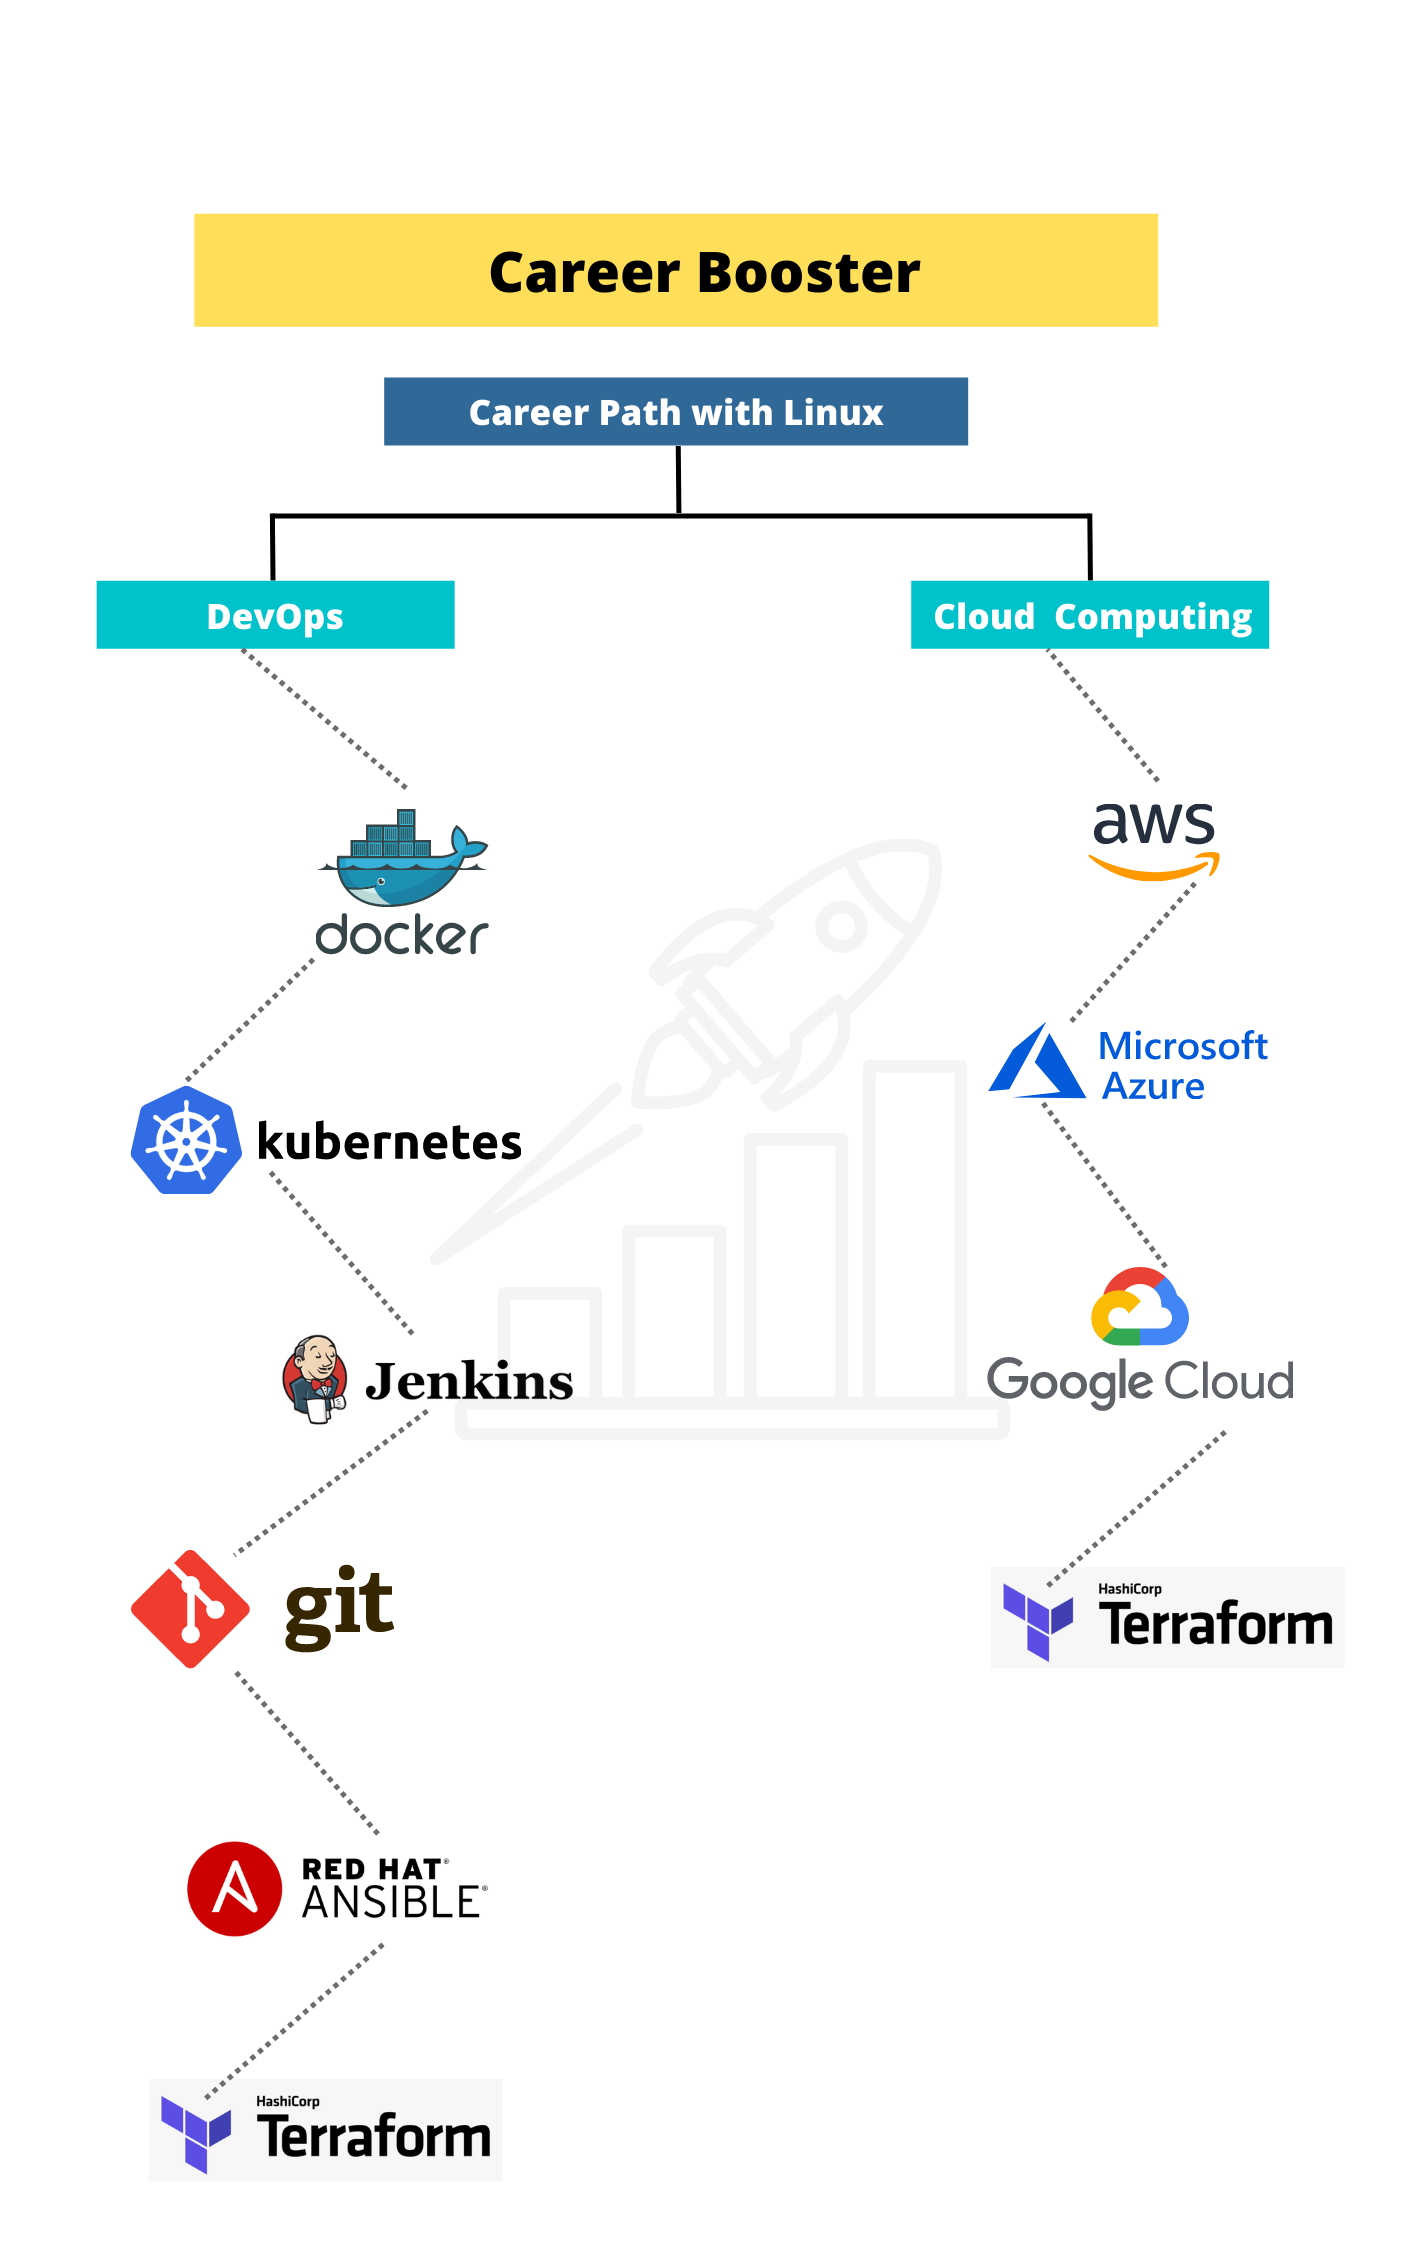
\includegraphics[scale=.38]{content/chapter1/images/career.png}
	\end{figure}
\end{flushleft}

\newpage


\chapterimage{index2.png} % Chapter heading image
\chapter{Introduction}
%-----------------------
\section{Introduction to Operating System}\index{Introduction to Operating System}

\setlength{\columnsep}{3pt}
\begin{flushleft}
	\bigskip
	\bigskip
	\begin{tcolorbox}[breakable,notitle,boxrule=1pt,colback=black,colframe=black]
	\color{white}
	\bigskip
	In this section, you are going to learn:
	\begin{enumerate}
		\item \textbf{What is an Operating System (OS)?}
		\item \textbf{Architecture of OS?}
		\item \textbf{Types of OS}
	\end{enumerate}	
	\bigskip
	Finally, there will be a \textbf{small excerise} on these topics to check your knowledge.
	\bigskip
	\end{tcolorbox}

	
	\bigskip
	\bigskip
	
	\begin{multicols}{2}
		\vspace*{\fill}
		\vspace*{\fill}
		\vspace*{\fill}
		\vspace*{\fill}
		\vspace*{\fill}
		\vspace*{\fill}
		\vspace*{\fill}
		\vspace*{\fill}
		\vspace*{\fill}
		
		\vfill \null
		\columnbreak
		So let's get started....
		
\includegraphics[scale=0.08]{content/linux_section.png}
	\end{multicols}	
	
\end{flushleft}

\newpage






\subsection{What is an Operating System (OS)?}\index{Introduction to Operating System!What is an Operating System (OS)?}

\begin{flushleft}
	An Operating System (OS) is an interface between a user and computer hardware.
	\bigskip
	\begin{figure}[h!]
		\centering
		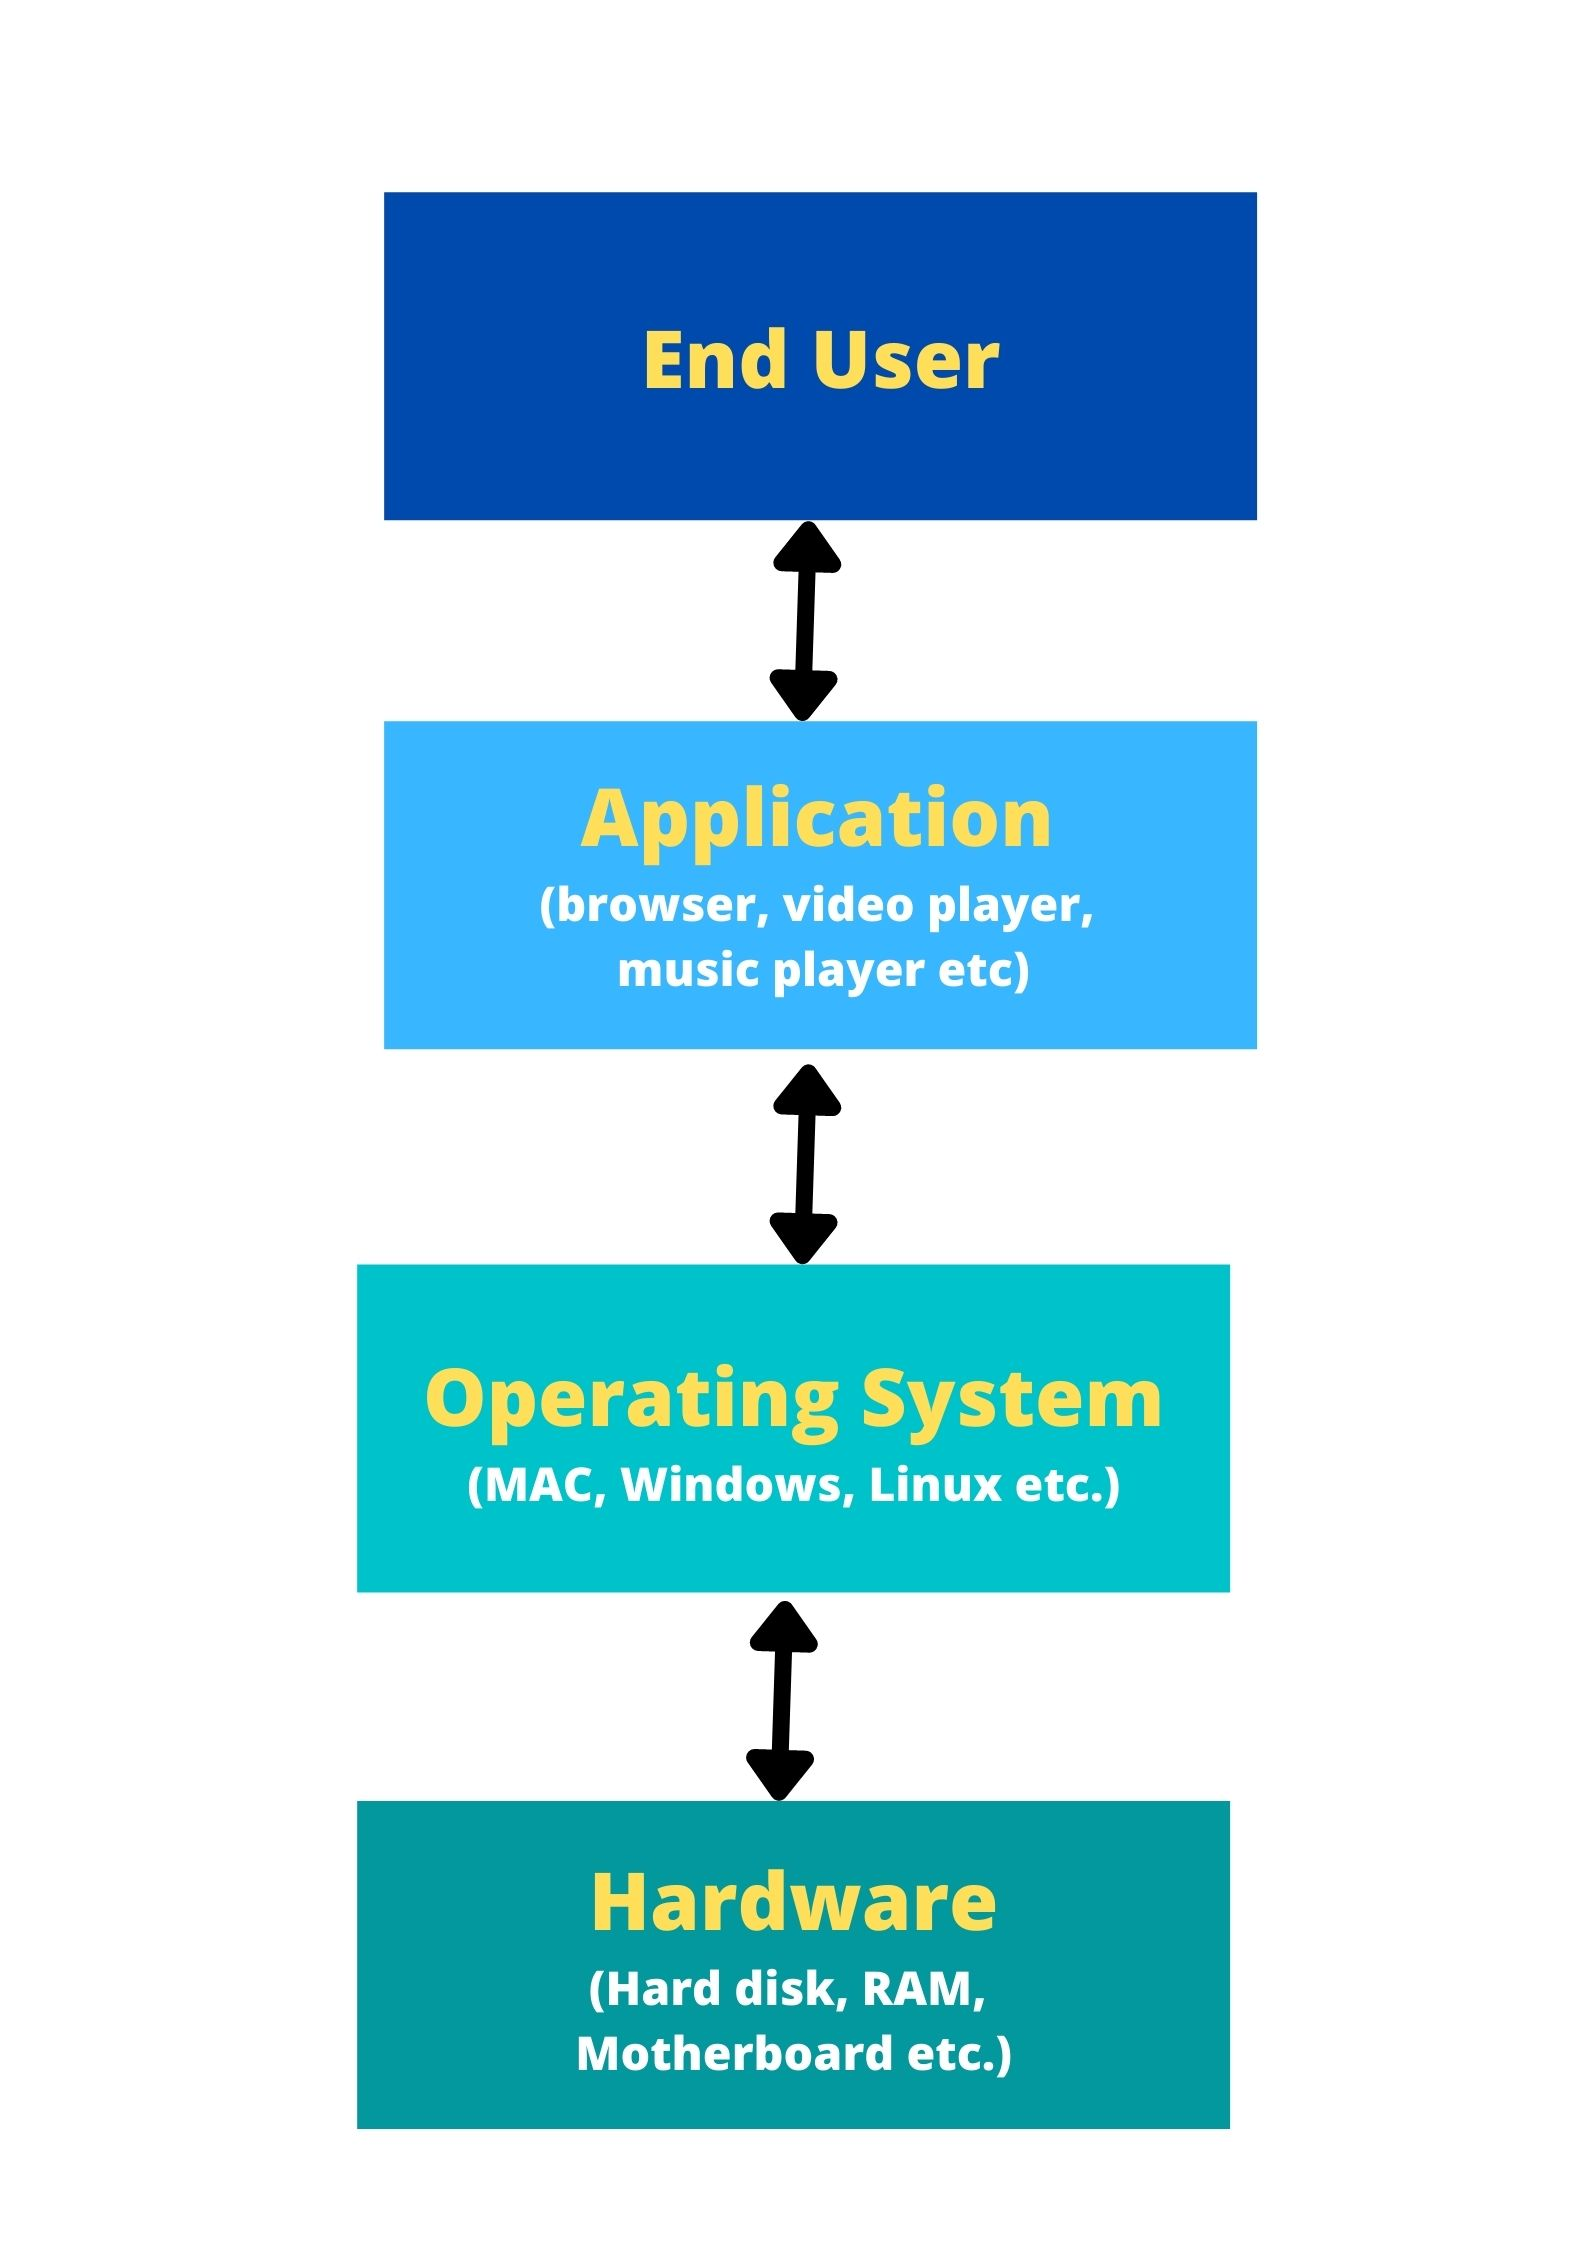
\includegraphics[scale=.3]{content/chapter1/images/os.jpg}
		\caption{Operating System}
		\label{fig:OS}
	\end{figure}
\end{flushleft}

\newpage


\subsection{Architecture of OS}\index{Introduction to Operating System!Architecture of OS}
\begin{flushleft}
	An OS consists of:
	\begin{itemize}
		\item Kernel
		\item Shell
		\item Applications
	\end{itemize}
	\begin{figure}[h!]
		\centering
		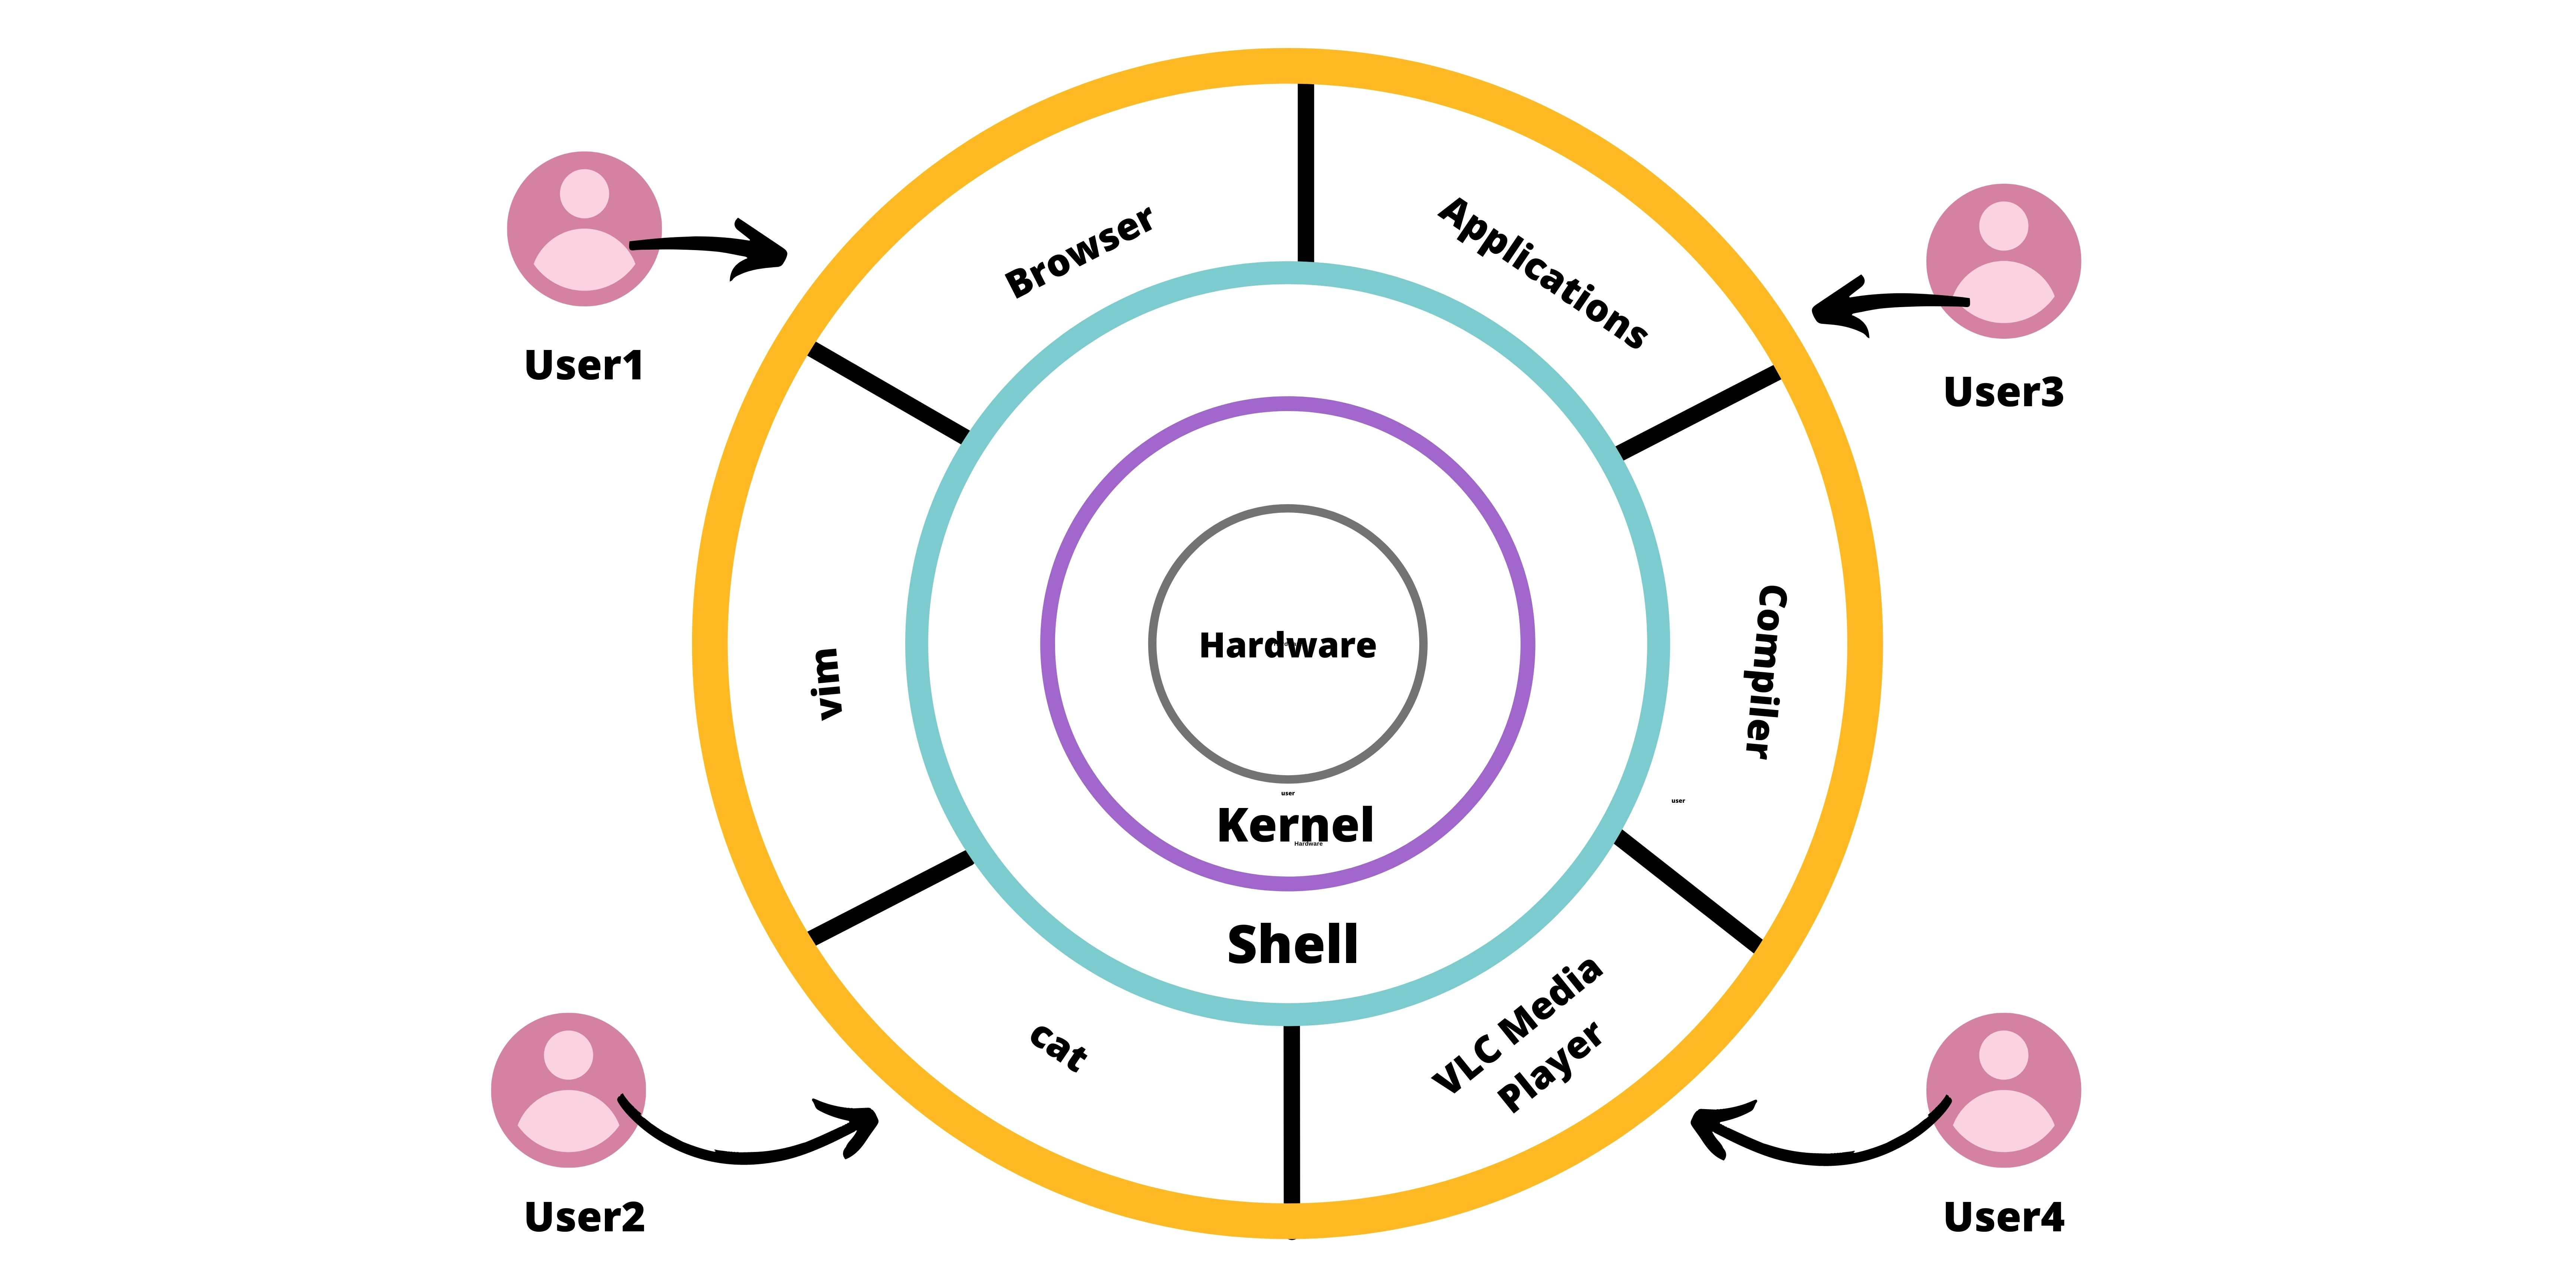
\includegraphics[scale=.08]{content/chapter1/images/os_structure.jpg}
		\caption{OS architecture}
		\label{fig:OS_Structure}
	\end{figure}
	Let's see each of these in detail.
	
	\newpage
	
	\begin{enumerate} 
		\item \textbf{Kernel} - 
		\begin{itemize}
			\item Establish communication between hardware and software.
			\begin{figure}[h!]
				\centering
				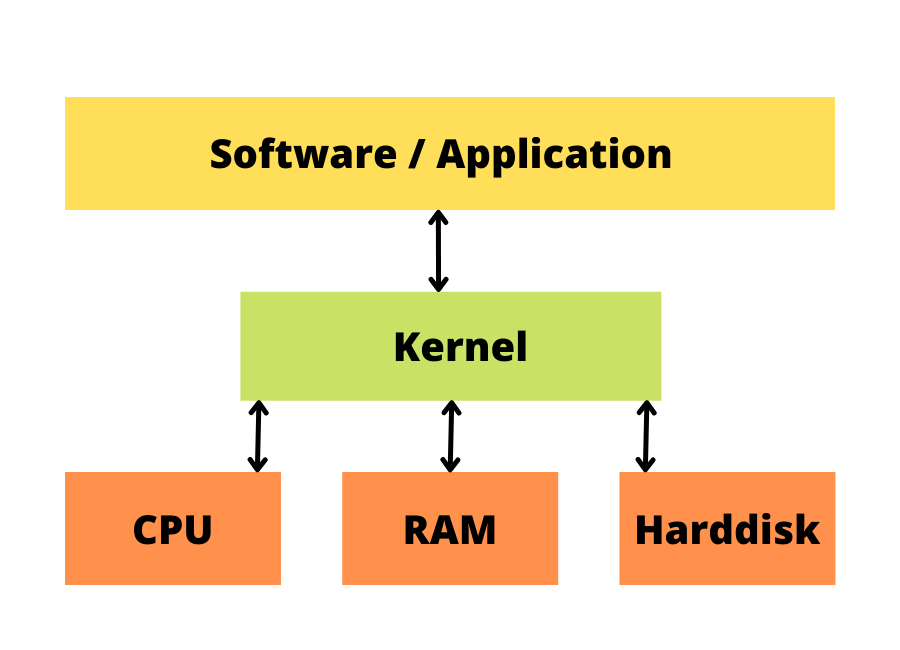
\includegraphics[scale=.4]{content/chapter1/images/kernel.png}
				\caption{Kernel}
				\label{fig:kernel}
			\end{figure}
			\item Kernel performs:
			\begin{itemize}
				\item \textbf{Process Management}: Manage CPU processes.
				\item \textbf{Device Management}: Interface between hardware and process.
				\item \textbf{Memory Management}: Manage RAM.
				\item \textbf{Handling system calls}: Provides the interface between the processes and OS.
			\end{itemize}			
		\end{itemize}
		\bigskip
		
		\item \textbf{Shell} - An interface to kernel that takes commands from user and executes them.
		\bigskip
		
		\item \textbf{Utilities/applications} - Programs that can be directly used by users.
	\end{enumerate}
\end{flushleft}

\newpage




\subsection{Types of OS}\index{Introduction to Operating System!Types of OS}
\setlength{\columnsep}{20pt}
\begin{flushleft}
	There are 3 types of OS:
	\begin{enumerate}
		\item 
		\begin{multicols}{2}
			\textbf{Server OS} - Designed for server computers that runs 24X7.
			\newline
			Eg:
			\begin{itemize}
				\item Linux server
				\item Windows server
				\item Mac OS X server
			\end{itemize}
			\vfill \null
			\columnbreak
			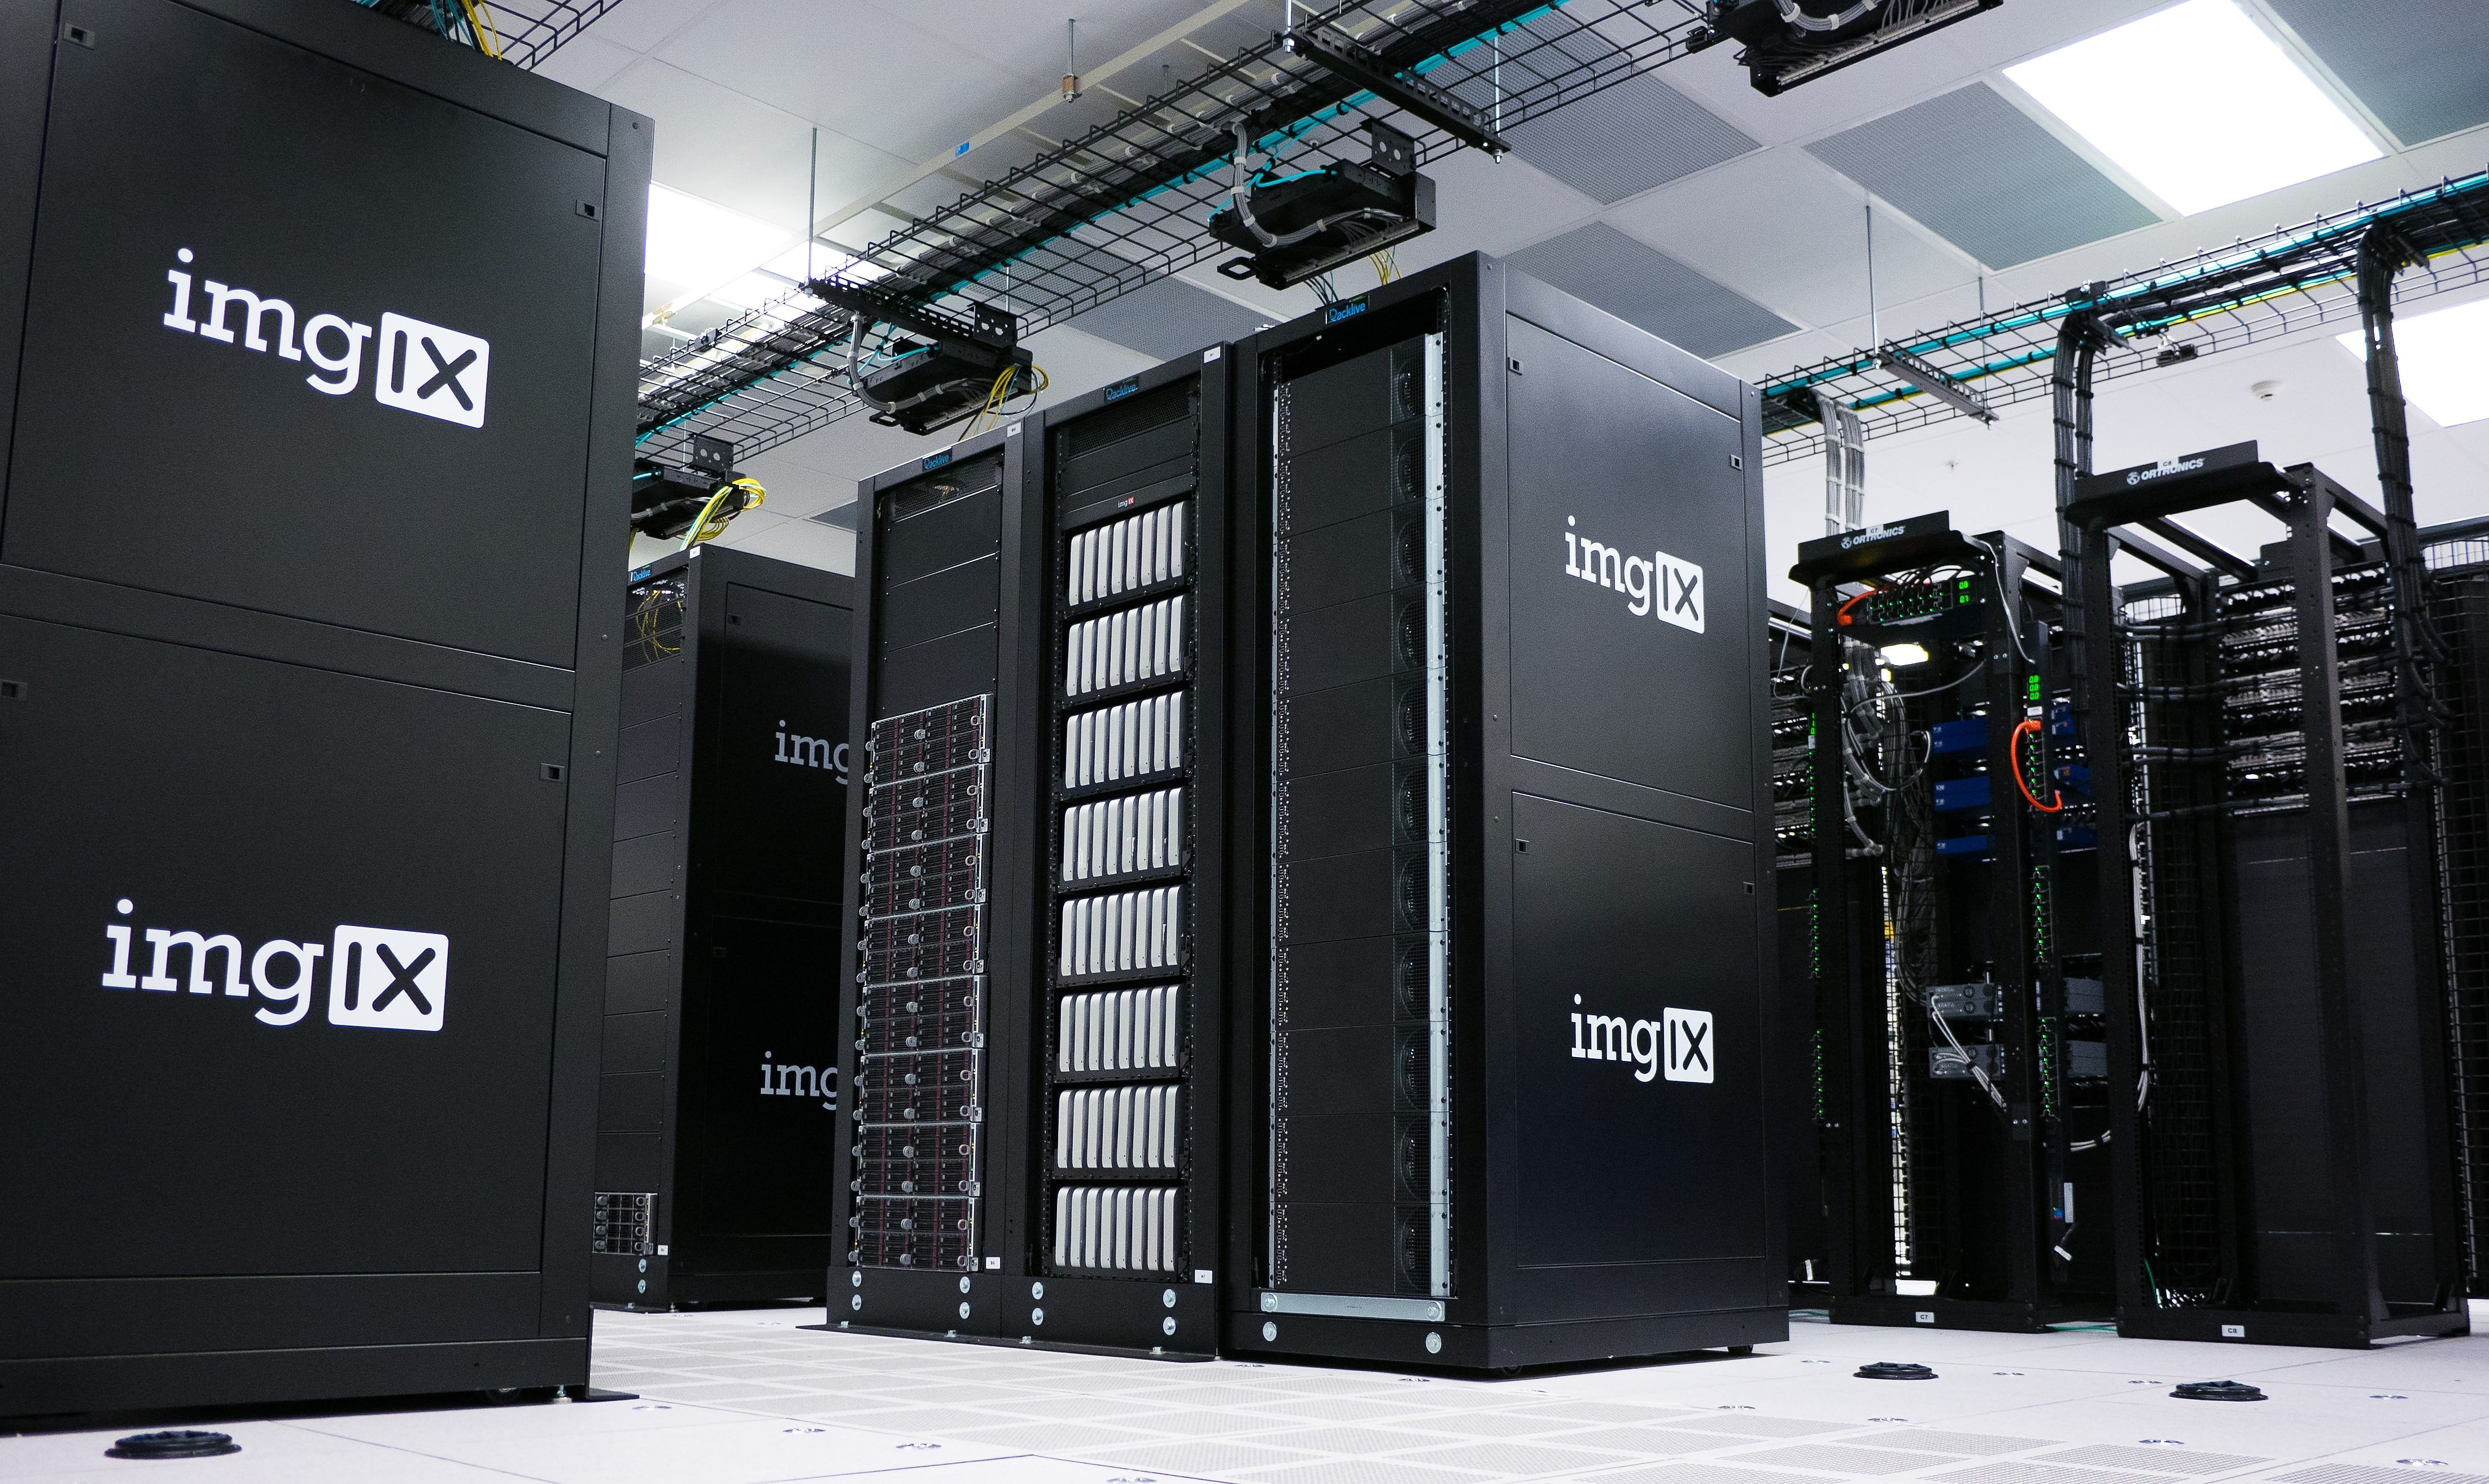
\includegraphics[scale=.03]{content/chapter1/images/server.jpg}
		\end{multicols}
		\vspace{-25pt}

\bigskip
		
		\item 
		\begin{multicols}{2}
			\textbf{Desktop OS} - Designed for personal computer.
			\newline
			Eg:
			\begin{itemize}
				\item Windows
				\item Mac OS
			\end{itemize}
			\vfill \null			
			\columnbreak
			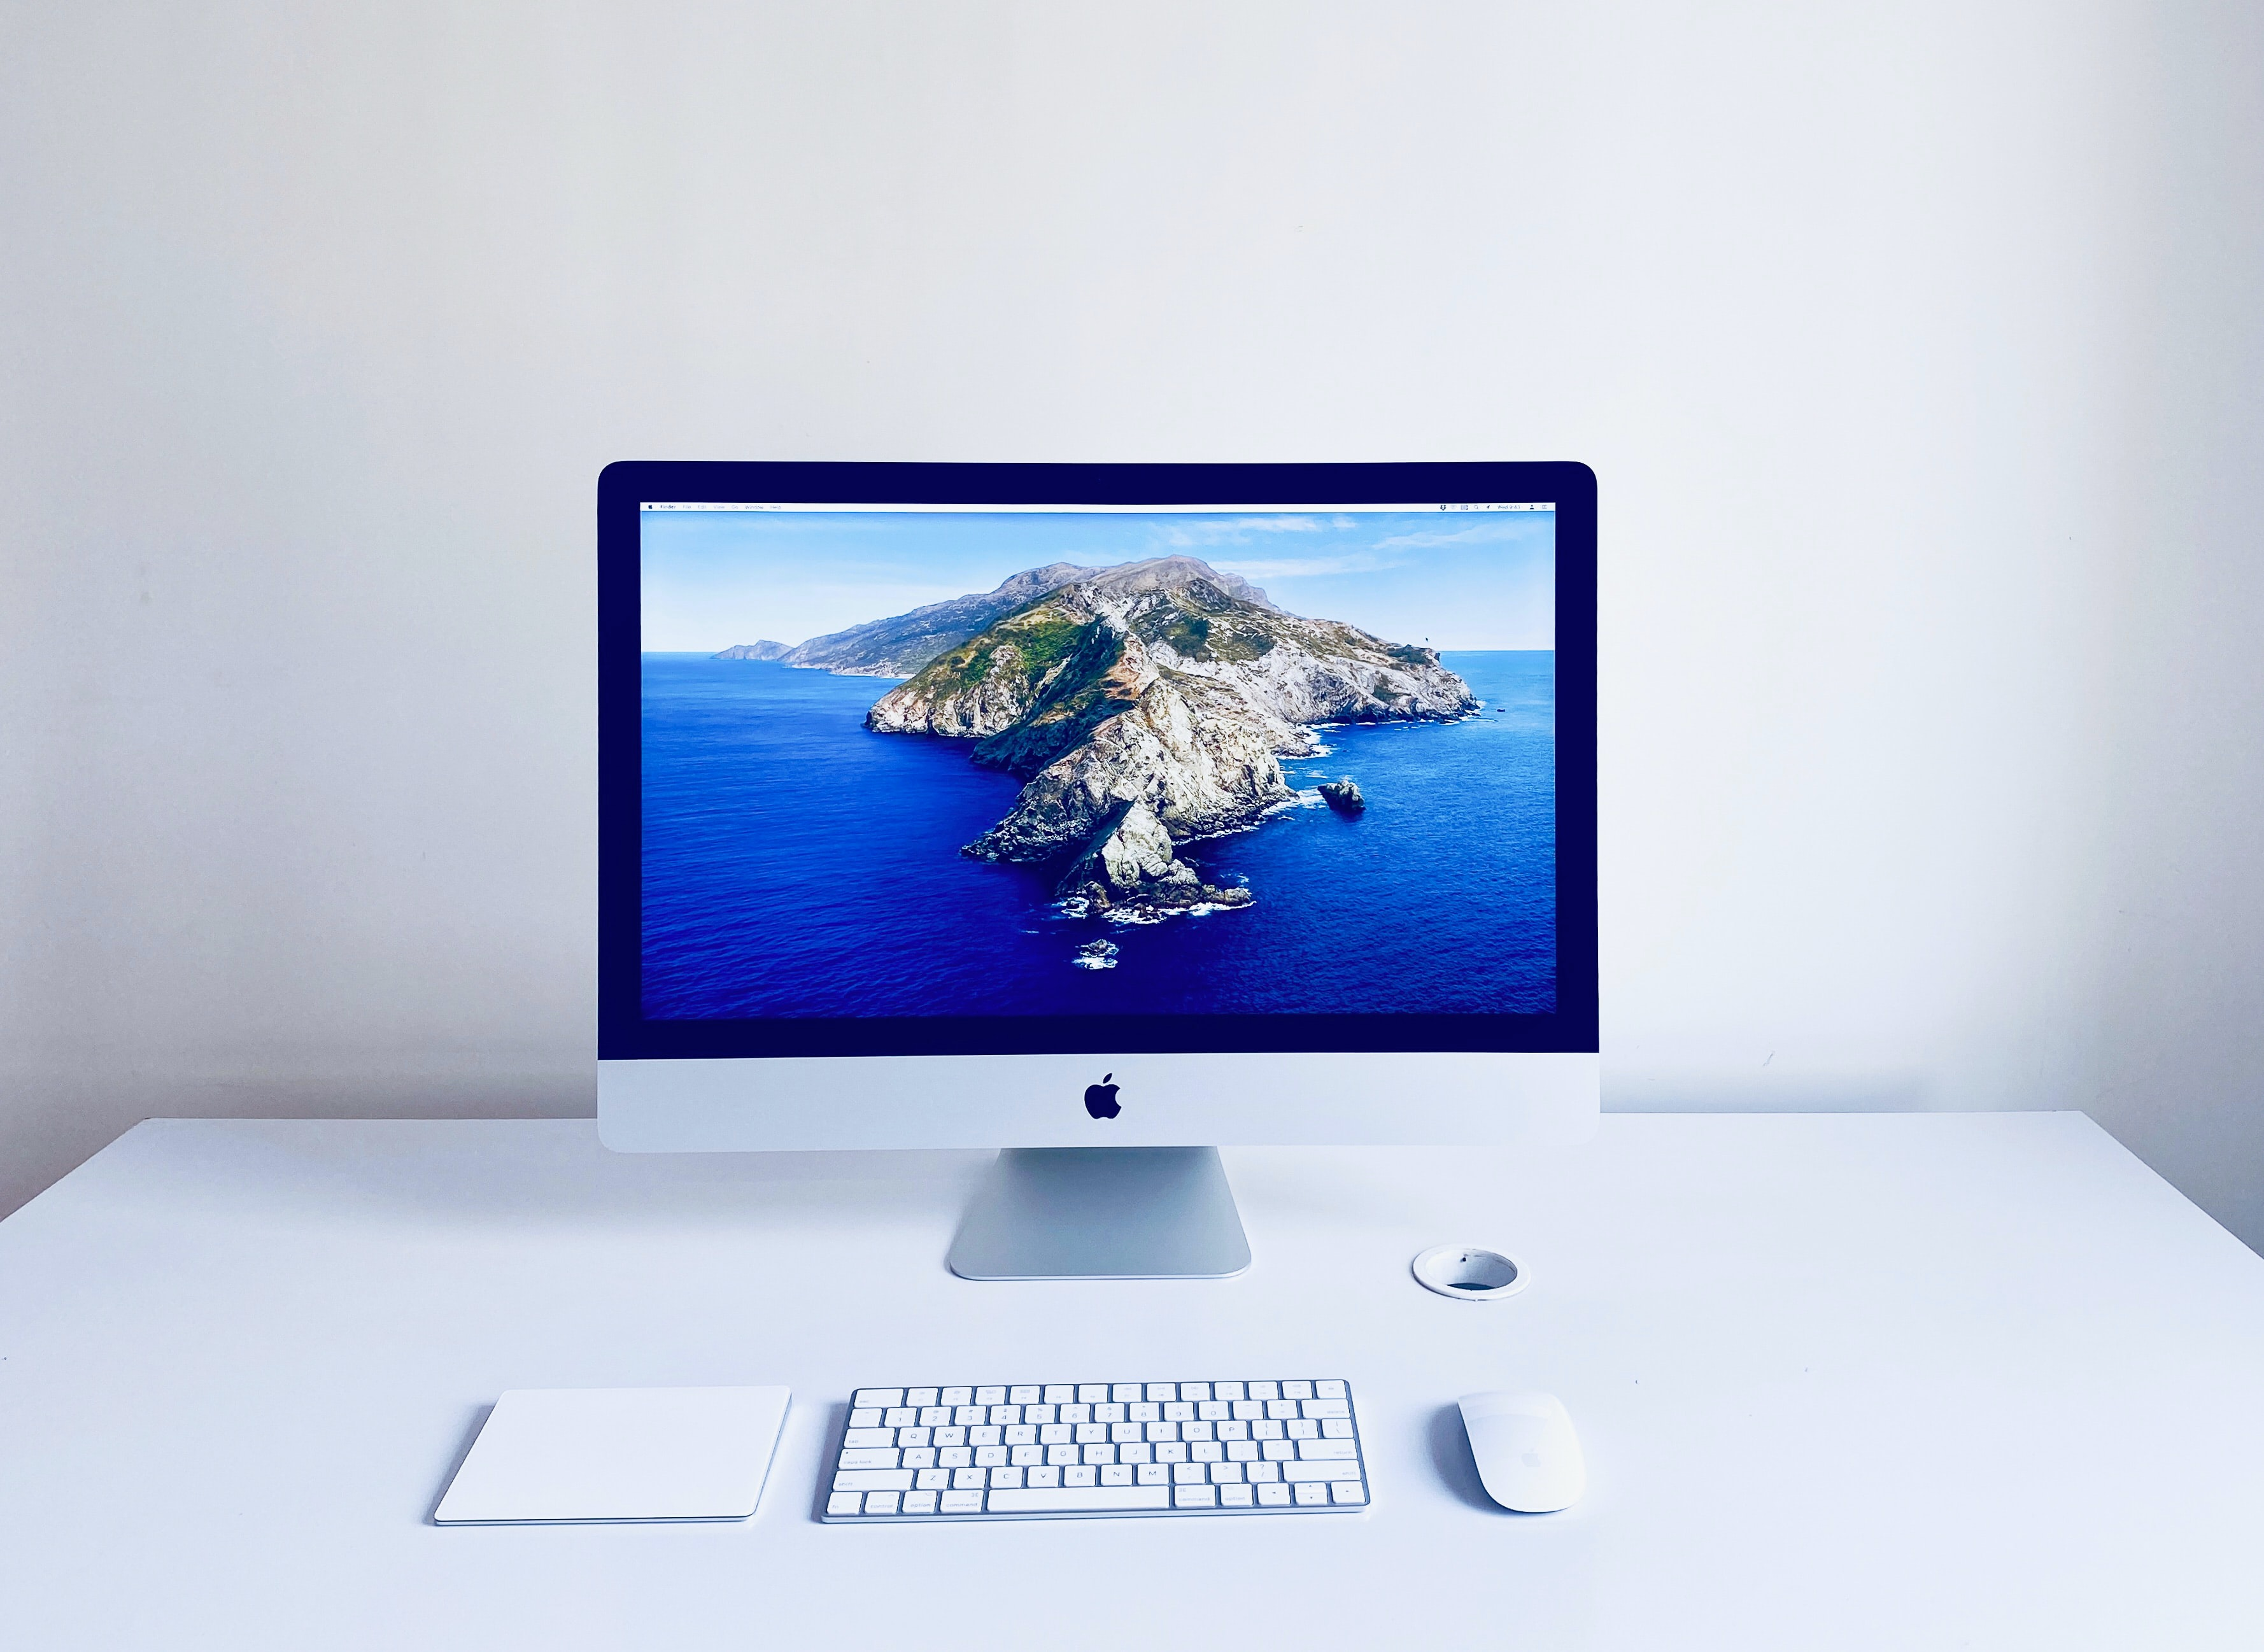
\includegraphics[scale=.03]{content/chapter1/images/desktop.jpg}
		\end{multicols}
		\vspace{-25pt}
		
\bigskip
		
		\item 
		\begin{multicols}{2}
			\textbf{Mobile OS} - Designed to run on mobile devices.
			\newline
			Eg:
			\begin{itemize}
				\item IPhone OS
				\item Windows mobile
				\item Anroid
			\end{itemize}
			\vfill \null			
			\columnbreak
			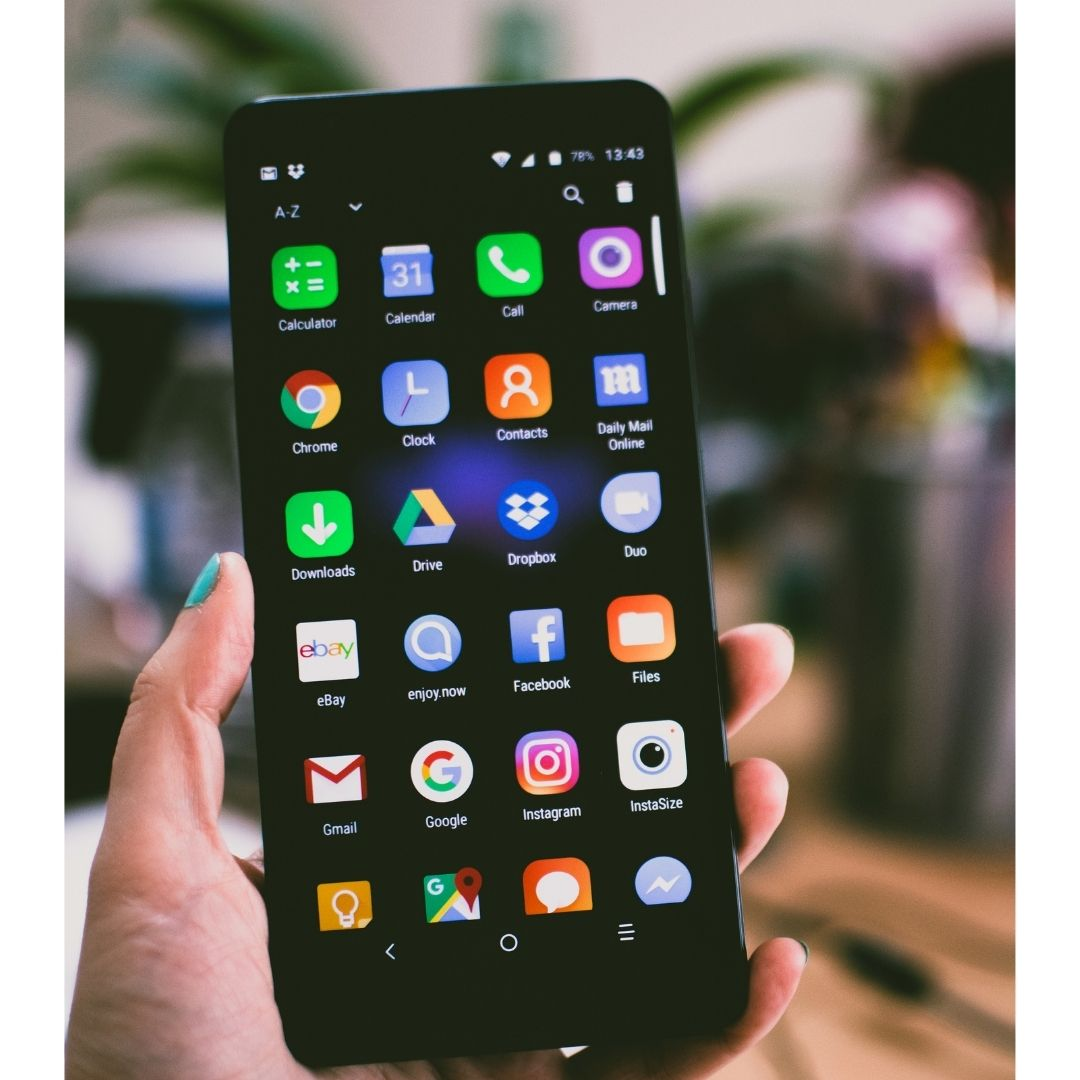
\includegraphics[scale=.12]{content/chapter1/images/mobile.jpg}
		\end{multicols}
		\vspace{-25pt}

		%\bigskip
	\end{enumerate}
\end{flushleft}

\newpage


\subsection{Practice}\index{Introduction to Operating System!Practice}
\begin{flushleft}
	
	\bigskip
	
	\begin{figure}[h!]
		\centering
		
\includegraphics[scale=.2]{content/practise.jpg}
	\end{figure}	
	\begin{enumerate}
		\item \textbf{What is an Operating System? (Select all that applies.)}
		\begin{enumerate}[label=(\alph*)]
			\item A software used for only gaming purpose.
			\item Collection of software that acts as an interface between a user and computer hardware. %correct
			\item OS consists of kernel to interact with hardware, shell and utilities. %correct
			\item OS is a software used for accounting purpose. %correct
			%\item \light{Handling system calls}
		\end{enumerate}
		\bigskip
		\bigskip
		\item \textbf{Which of the following are the functions of a kernel? (Select all that applies.)}
		\begin{enumerate}[label=(\alph*)]
			\item Perform memory management by keeping track of memory. %correct
			\item Perform hardware management. %correct
			\item Establish communication between hardware and software. %correct
			\item Control all processes of the OS. %correct
		\end{enumerate}
		\bigskip
		\bigskip
		\item \textbf{State whether true or false. Kernel is an interface between hardware and software.}
		\begin{enumerate}[label=(\alph*)]
			\item True %correct
			\item False
		\end{enumerate}
	\end{enumerate}
	

\end{flushleft}

\newpage

\section{Introduction to Linux}\index{Introduction to Linux}
\setlength{\columnsep}{3pt}
\begin{flushleft}
	\bigskip
	\bigskip
	\begin{tcolorbox}[breakable,notitle,boxrule=1pt,colback=black,colframe=black]
		\color{white}
		\bigskip
		In this section, you are going to learn:
		\begin{enumerate}
			\item \textbf{What is Open Source Software (OSS)?}
			\item \textbf{What is Linux OS?}
			\item \textbf{Linux OS V/S Windows OS}
			\item \textbf{What is console, terminal, command line \& shell?}
			\item \textbf{Linux distributions}
		\end{enumerate}	
		Finally, there will be a \textbf{small excerise} on these topics to check your knowledge.
		\bigskip
	\end{tcolorbox}
	\bigskip
	\bigskip
	\begin{multicols}{2}
		\vspace*{\fill}
		\vspace*{\fill}
		\vspace*{\fill}
		\vspace*{\fill}
		\vspace*{\fill}
		\vspace*{\fill}
		\vfill \null
		\columnbreak
		So let's get started....
		
\includegraphics[scale=0.07]{content/linux_section.png}
	\end{multicols}
\end{flushleft}
\newpage

\subsection{What is Open Source Software (OSS)?}\index{Introduction to Linux!What is open source software(OSS)?}
\setlength{\columnsep}{5pt}
\begin{flushleft}
	\paragraph{}
	\begin{itemize}
		\item Open source software (OSS) is code that is publicly accessible.
		\item OSS is:
		\begin{itemize}
			\item \textbf{Free to use}
			\item \textbf{Free to modify}
			\item \textbf{Free to distribute}
		\end{itemize}
	\end{itemize}	
	\bigskip
	\bigskip
	\bigskip
	\begin{figure}[h!]
		\centering
		
\includegraphics[scale=.1]{content/chapter1/images/open.png}
		\caption{Open Source Software Logo}
		\label{fig:opensource}
	\end{figure}
	Some of the OSS:
	\begin{figure}[h!]
		\centering
		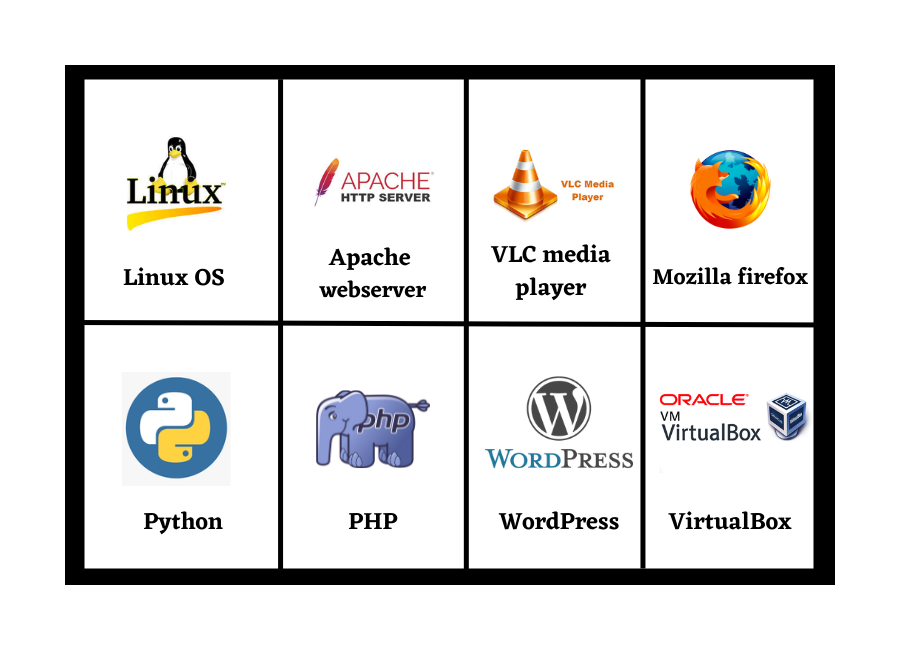
\includegraphics[scale=.4]{content/chapter1/images/opensource.png}
		\caption{Open Source Softwares}
		\label{fig:opensource1}
	\end{figure}
	
\end{flushleft}
\newpage

\subsection{What is Linux OS?}\index{Introduction to Linux!Linux V/S Windows}
\setlength{\columnsep}{5pt}
\begin{flushleft}
	\paragraph{}
	\begin{itemize}
		\item Linux® is an open source operating system. 
		\item Created as a hobby by Linus Torvalds in 1991, as alternative of the MINIX OS (which is variant of Unix).
		\item Developed for \textbf{ personal computers, servers, mainframes, mobile devices and embedded devices}.
	\end{itemize}	
	\begin{figure}[h!]
		\centering
		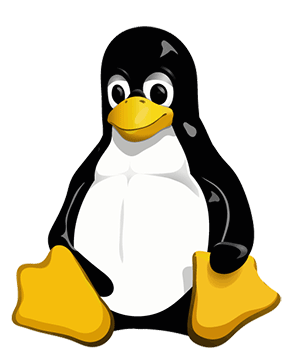
\includegraphics[scale=.5]{content/chapter1/images/tux.png}
		\caption{Tux, the Linux mascot, by Larry Ewing}
		\label{fig:mascot}
	\end{figure}	
\end{flushleft}

\newpage

\subsection{Linux OS v/s Windows OS}\index{Introduction to Linux!Linux V/S Windows}
\setlength{\columnsep}{5pt}

\begin{flushleft}
	\paragraph{}
		%\begin{tabulary}{1.0\textwidth}{C|C|C|p{10em}}
		
		
		\begin{tabulary}{1.0\textwidth}{|p{14em}|p{14em}|}
			\toprule
			\textbf{Linux OS} & \textbf{Windows OS}\\
			\midrule
			Open source OS & Closed source OS \\
			\hline
			Free of cost & Not free \\
			\hline
			File names are case-sensitive & File names are case-insensitive \\
			\hline
			More efficient in resource usage & Less efficient in resource usage\\
			\hline
			More security, no need to install anti-virus & Less security, need to install anti-virus\\
			\hline
			Used for devops, programming, database, cloud-computing, big data hadoop etc & Used mostly for house hold purpose\\
			\bottomrule
		\end{tabulary}

		\label{tab:example} % Unique label used for referencing the table in-text
		%\addcontentsline{toc}{table}{Table \ref{tab:example}} % Uncomment to add the table to the table of contents
		

				
\end{flushleft}

\newpage
\subsection{Understanding console, terminal, command line and shell}\index{Introduction to Linux!Understanding console, terminal, command line and shell}
\setlength{\columnsep}{5pt}
\begin{flushleft}
	\bigskip
	\bigskip
	\paragraph{What is a console and terminal?}
	\begin{itemize}
		\item A console is a device with a screen and keyboard combined inside it.
		\item Terminal is the software program inside the console.
			\begin{figure}[h!]
			\centering
			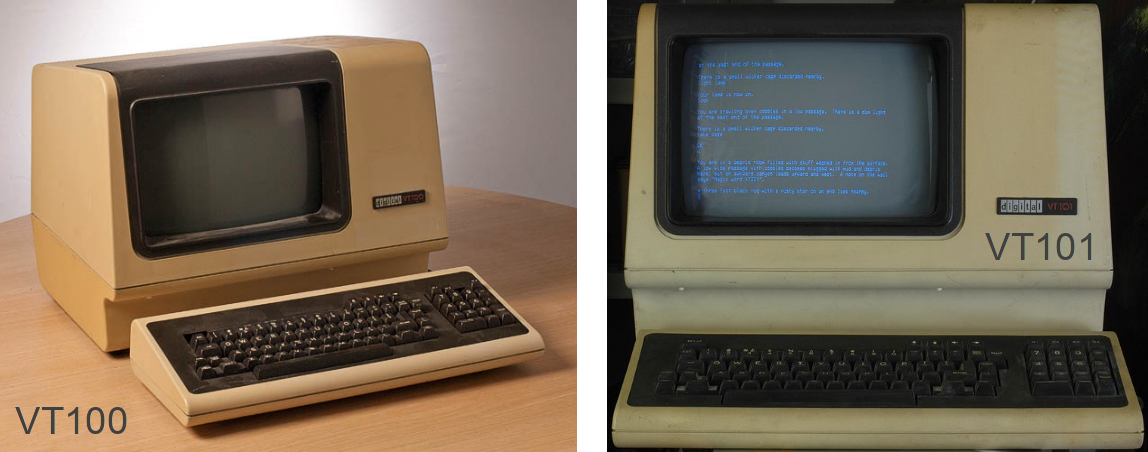
\includegraphics[width=5cm]{content/chapter1/images/console.png}
			\caption{VT terminals - The first console with terminal}%
			\label{fig:example}%
			\end{figure}		
	\end{itemize}
% figure side by side
%	\begin{figure}[h!]
%		\centering
%		\subfloat[\centering VT terminals]{{
%		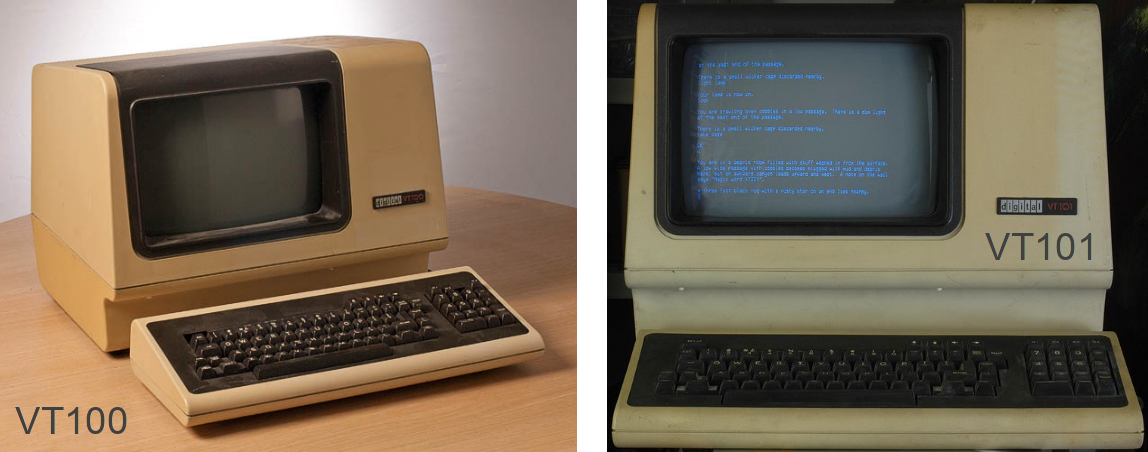
\includegraphics[width=10cm]{content/chapter1/images/console.png}}}%
%		\qquad
%		\subfloat[\centering RS-232 connector to connect console to terminal]{{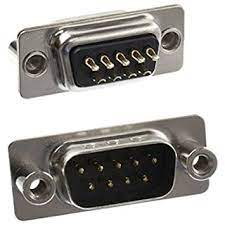
\includegraphics[width=5cm]{content/chapter1/images/connector.jpeg} }}%
%		\caption{2 VT terminal and connector}%
%		\label{fig:example}%
%	\end{figure}

	\paragraph{What is a command line?}
	\begin{itemize}
		\item It is a blank line and cursor on the screen, allowing the user to type commands to execute.
	
		\begin{figure}[h!]
			\centering
			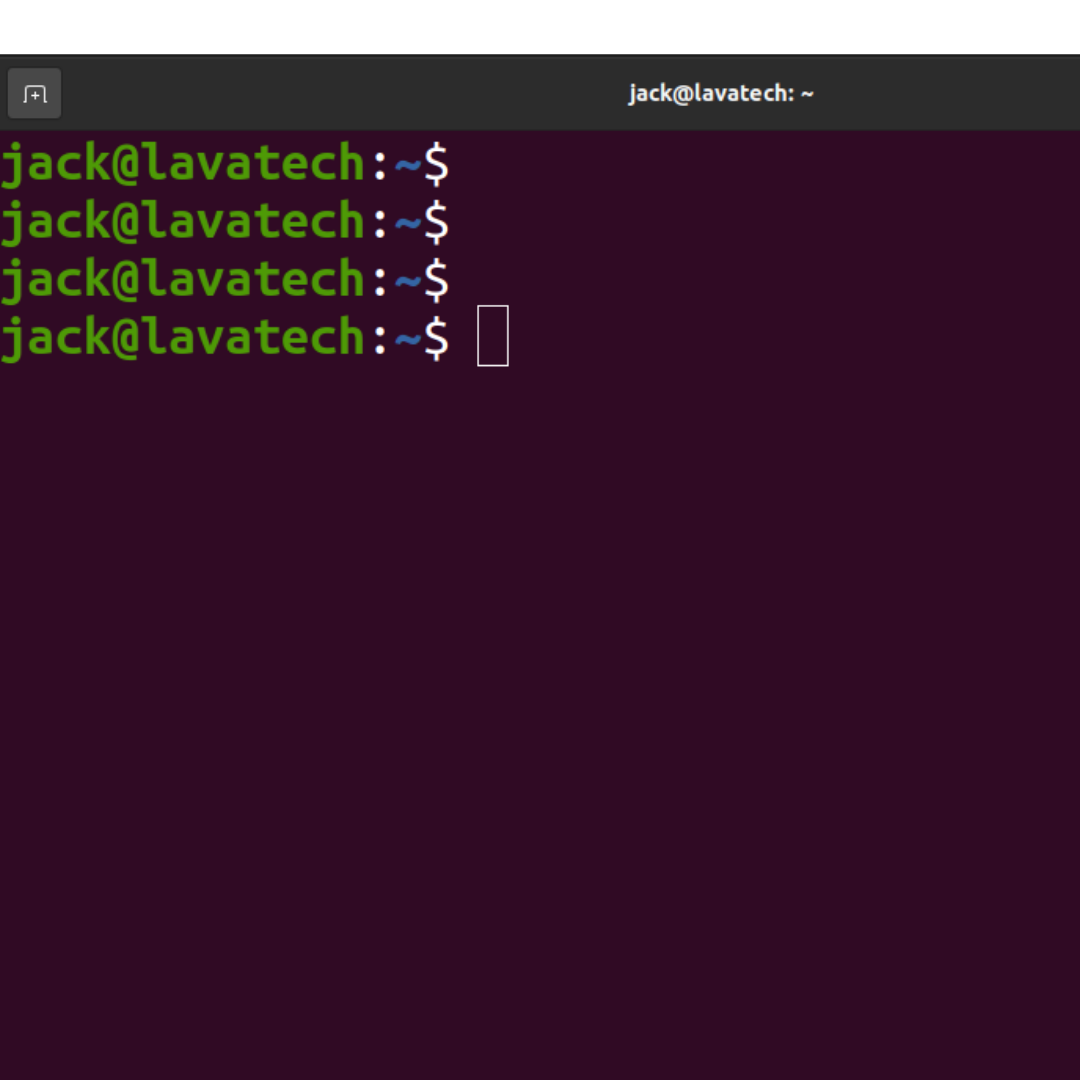
\includegraphics[scale=.18]{content/chapter1/images/commandline.png}
			\caption{Linux command line}
			\label{fig:commandline}
		\end{figure}	
	\end{itemize}
	\paragraph{What is a shell?}
	\begin{itemize}
		\item Shell is an interface to kernel.
		\item It executes Linux commands \& display it's result.
		\item Eg:
		\begin{itemize}
			\item Shell in Linux OS: bash, fish, zsh, ksh, sh, tsch
			\item Shell in Windows OS: PowerShell, pwsh
		\end{itemize}
	\end{itemize}		
\end{flushleft}

\newpage

%\subsection{Linux in server industry}\index{Introduction to Linux!Linux in server industry}
%\setlength{\columnsep}{5pt}
\begin{flushleft}
	\bigskip
	\bigskip
	\paragraph{What is a console and terminal?}
	\begin{itemize}
		\item A console is a device with a screen and keyboard combined inside it.
		\item Terminal is the software program inside the console.
			\begin{figure}[h!]
			\centering
			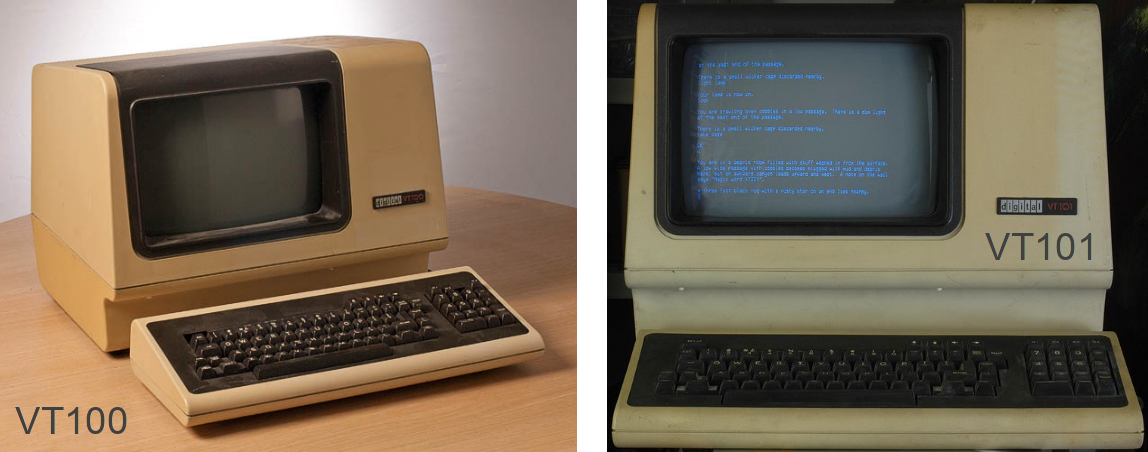
\includegraphics[width=5cm]{content/chapter1/images/console.png}
			\caption{VT terminals - The first console with terminal}%
			\label{fig:example}%
			\end{figure}		
	\end{itemize}
% figure side by side
%	\begin{figure}[h!]
%		\centering
%		\subfloat[\centering VT terminals]{{
%		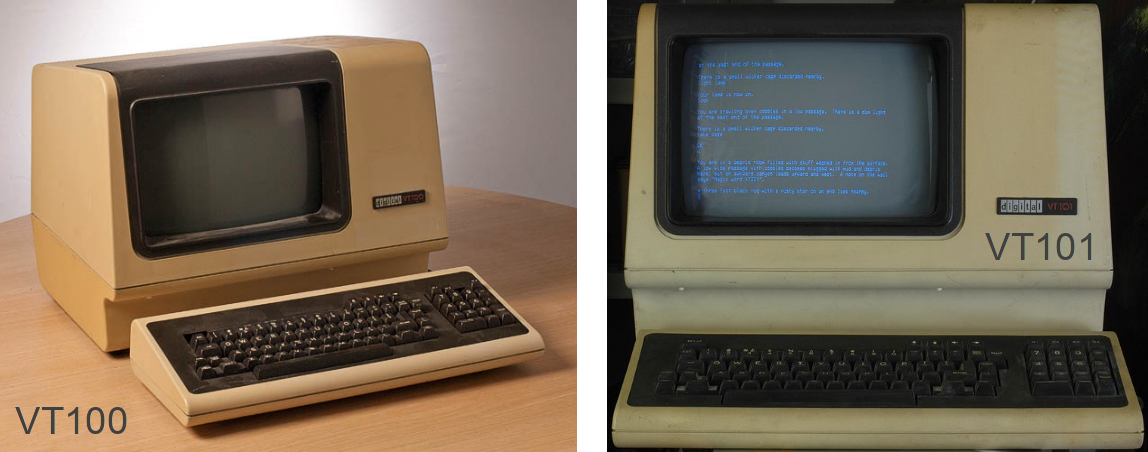
\includegraphics[width=10cm]{content/chapter1/images/console.png}}}%
%		\qquad
%		\subfloat[\centering RS-232 connector to connect console to terminal]{{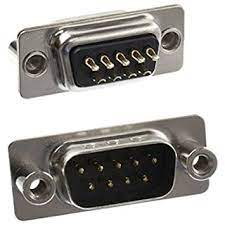
\includegraphics[width=5cm]{content/chapter1/images/connector.jpeg} }}%
%		\caption{2 VT terminal and connector}%
%		\label{fig:example}%
%	\end{figure}

	\paragraph{What is a command line?}
	\begin{itemize}
		\item It is a blank line and cursor on the screen, allowing the user to type commands to execute.
	
		\begin{figure}[h!]
			\centering
			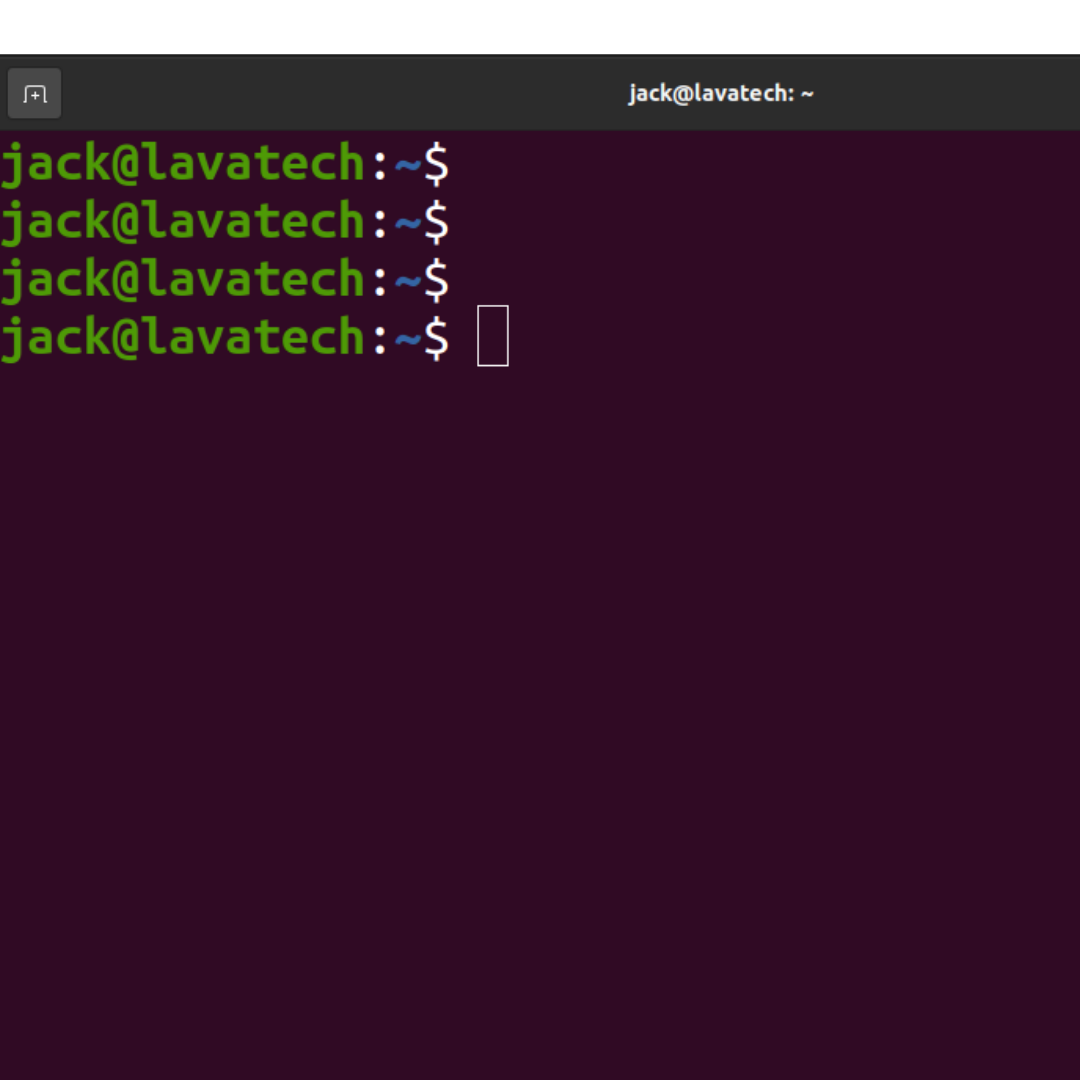
\includegraphics[scale=.18]{content/chapter1/images/commandline.png}
			\caption{Linux command line}
			\label{fig:commandline}
		\end{figure}	
	\end{itemize}
	\paragraph{What is a shell?}
	\begin{itemize}
		\item Shell is an interface to kernel.
		\item It executes Linux commands \& display it's result.
		\item Eg:
		\begin{itemize}
			\item Shell in Linux OS: bash, fish, zsh, ksh, sh, tsch
			\item Shell in Windows OS: PowerShell, pwsh
		\end{itemize}
	\end{itemize}		
\end{flushleft}

\newpage

\subsection{Linux distributions}\index{Introduction to Linux!Linux distributions}
\setlength{\columnsep}{5pt}
\begin{flushleft}
	\paragraph{}
	\begin{itemize}
		\item A Linux distribution (or distro) is made from the \textbf{Linux kernel and collection of software}.
		\item Almost one thousand Linux distributions exist.
		\item Free and community managed distributions are:
		\begin{figure}[h!]
			\centering
			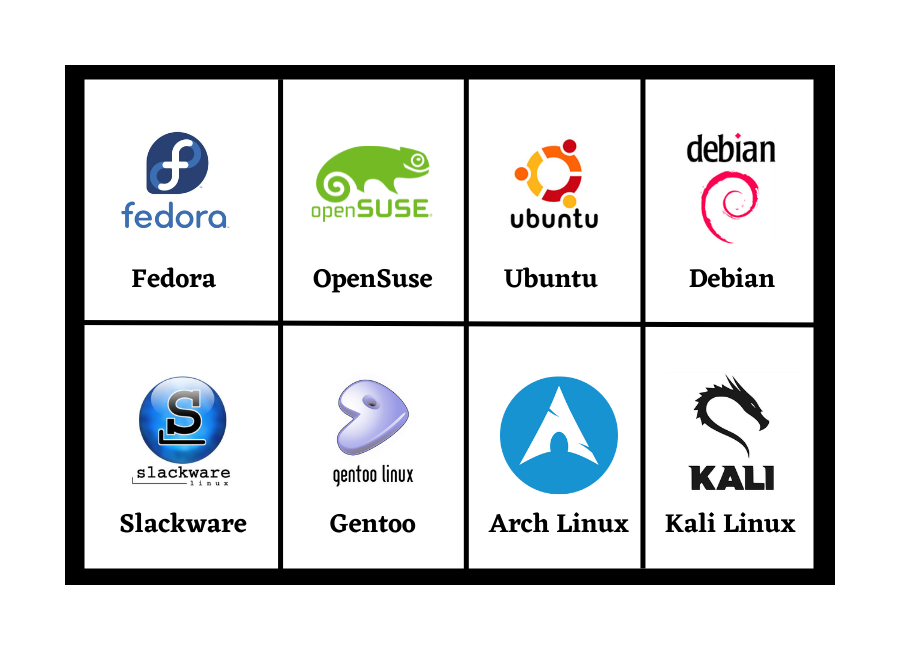
\includegraphics[scale=0.4]{content/chapter1/images/distro.png}
			\caption{Linux distributions}
			\label{fig:distro1}
		\end{figure}
		
		\item Popular commercially backed distributions are:
		\begin{figure}[h!]
			\centering
			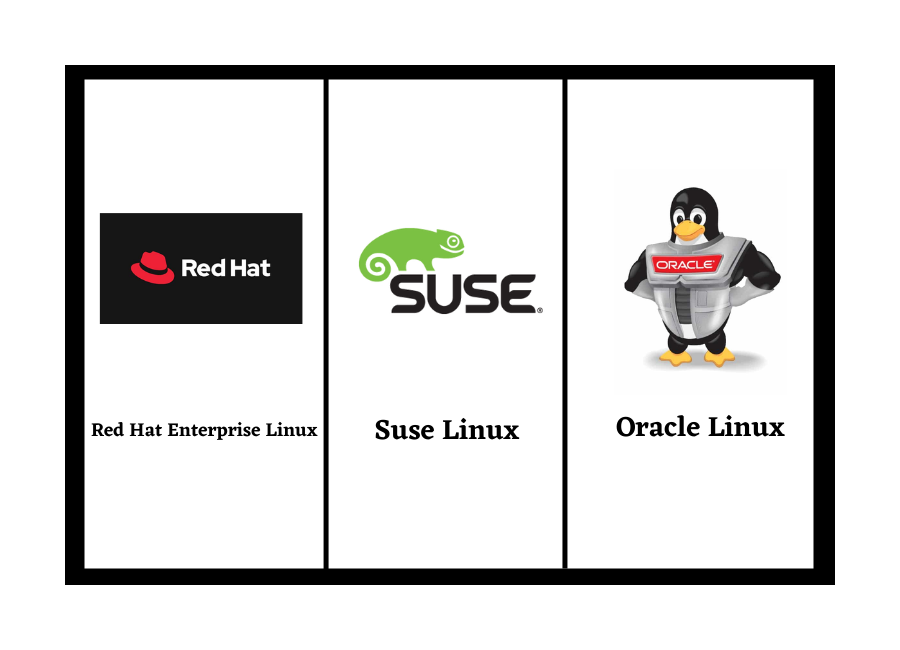
\includegraphics[scale=0.3]{content/chapter1/images/distro2.png}
			\caption{Commercial Linux distributions}
			\label{fig:distro2}
		\end{figure}

	\end{itemize}

	\newpage
	\paragraph{What is upstream and downstream?}
	\begin{itemize}
		\item The term 'upstream' refers to the \textbf{original version of a software}.
		\item Downstream is the \textbf{refined product code} based on original software version.
		\item Eg:
		\begin{itemize}
			\item \textbf{Fedora} is the upstream to \textbf{Red Hat Enterprise Linux (RHEL)}.
			\item \textbf{Debian} is the upstream to \textbf{Ubuntu}.
		\end{itemize}
	\end{itemize}
\end{flushleft}
\newpage

\subsection{Practice}\index{Introduction to Linux!Practice}
\setlength{\columnsep}{3pt}
\begin{flushleft}
	\paragraph{}

	\bigskip

	\begin{figure}[h!]
		\centering
		
\includegraphics[scale=.2]{content/practise.jpg}
	\end{figure}	
	
	\begin{enumerate}
		\item \textbf{Which of the following are Open Source Software (OSS)? (Select all that applies.)}
		\begin{enumerate}[label=(\alph*)]
			\item Python %correct
			\item Linux % correct
			\item Apache webserver %correct
			\item MySQL %correct
		\end{enumerate}
		\bigskip
		\bigskip
		\item \textbf{State whether true or false. OSS is free to use, develop, modify and distribute for personal and professional use.}
		\begin{enumerate}[label=(\alph*)]
			\item True  %correct
			\item False
		\end{enumerate}
		\bigskip
		\bigskip
		\item \textbf{Select all statement true for Linux OS.}
		\begin{enumerate}[label=(\alph*)] 
			\item Linux is OSS developed by Linus Torvalds. %correct
			\item Linux OS cannot be used for house-hold use.
			\item Linux OS is variant of MINIX OS.    %correct
			\item Linux is desgined for servers and mainframes computer.   %correct
		\end{enumerate}
		\bigskip
		\bigskip
		\newpage
		\item \textbf{Select all statement that are true about Linux and Windows OS.}
		\begin{enumerate}[label=(\alph*)]
			\item File names are case sensitive in Linux OS and case-insensitive in Windows OS.  %correct
			\item Linux OS is less secure than Windows OS.   
			\item Linux OS is OSS while Windows OS is closed source OS.   %correct
			\item Windows OS is expensive compared to Linux OS.   %correct
		\end{enumerate}
		\bigskip
		\bigskip
		\item \textbf{Select all statement that are true about shell.}
		\begin{enumerate}[label=(\alph*)]
			\item Bash and ksh are types of shell used in Linux OS.  %correct
			\item Shell takes command from terminal and supplies it to kernel for processing.  %correct
			\item Shell is an interface to kernel. %correct
			\item Powershell is an example of shell used in Windows OS.  %correct
		\end{enumerate}
		\bigskip
		\bigskip
		\item \textbf{State whether true or false. Fedora is upstream of RHEL.}
		\begin{enumerate}[label=(\alph*)]
			\item True   %correct
			\item False   
		\end{enumerate}
	\end{enumerate}

	
\end{flushleft}
\newpage



%--------------	--------


%--------------------------------------------------------------------------
%	CHAPTER 2
%-------------------------------------------------------------------------

\chapterimage{index3.png} % Table of contents heading image
\chapter{Linux Basics}
%-----------------------
\section{Linux directory structure}\index{Linux directory structure}
\setlength{\columnsep}{3pt}
\begin{flushleft}
	\bigskip
	\bigskip
	\begin{tcolorbox}[breakable,notitle,boxrule=1pt,colback=black,colframe=black]
		\color{white}
		\bigskip
		In this section, you are going to learn:
		\begin{enumerate}
			\item \textbf{Filesystem Hierarchy Standard (FHS)}
			\item \textbf{Important directories in FHS}
			\item \textbf{Some shortcuts to use in Linux OS}
		\end{enumerate}	
		\bigskip
		Finally, there will be a \textbf{small excerise} on these topics to check your knowledge.
		\bigskip
	\end{tcolorbox}
	
	
	\bigskip
	\bigskip
	
	\begin{multicols}{2}
		\vspace*{\fill}
		\vspace*{\fill}
		\vspace*{\fill}
		\vspace*{\fill}
		\vspace*{\fill}
		\vspace*{\fill}
		\vspace*{\fill}
		\vspace*{\fill}
		\vspace*{\fill}
		
		\vfill \null
		\columnbreak
		So let's get started....
		
\includegraphics[scale=0.08]{content/linux_section.png}
	\end{multicols}	
	
\end{flushleft}

\newpage






\subsection{Filesystem Hierarchy Standard (FHS)}\index{Linux directory structure!Filesystem Hierarchy Standard (FHS)}

\begin{flushleft}
	\begin{itemize}
		\item If you’re coming from Windows, you must be aware of C: drive, D: drive etc.
		\item In Linux, there is \textbf{no} C: or D: drive. 
		\item Linux have standard directory structure called Filesystem Hierarchy Standard (FHS).
	\end{itemize}
	
	\begin{tcolorbox}[breakable,notitle,boxrule=-1pt,colback=yellow,colframe=yellow]
		\color{black}
		\bigskip
		Note: Folder and directory means the same!
		\bigskip
	\end{tcolorbox}
	
	\bigskip
	\begin{figure}[h!]
		\centering
		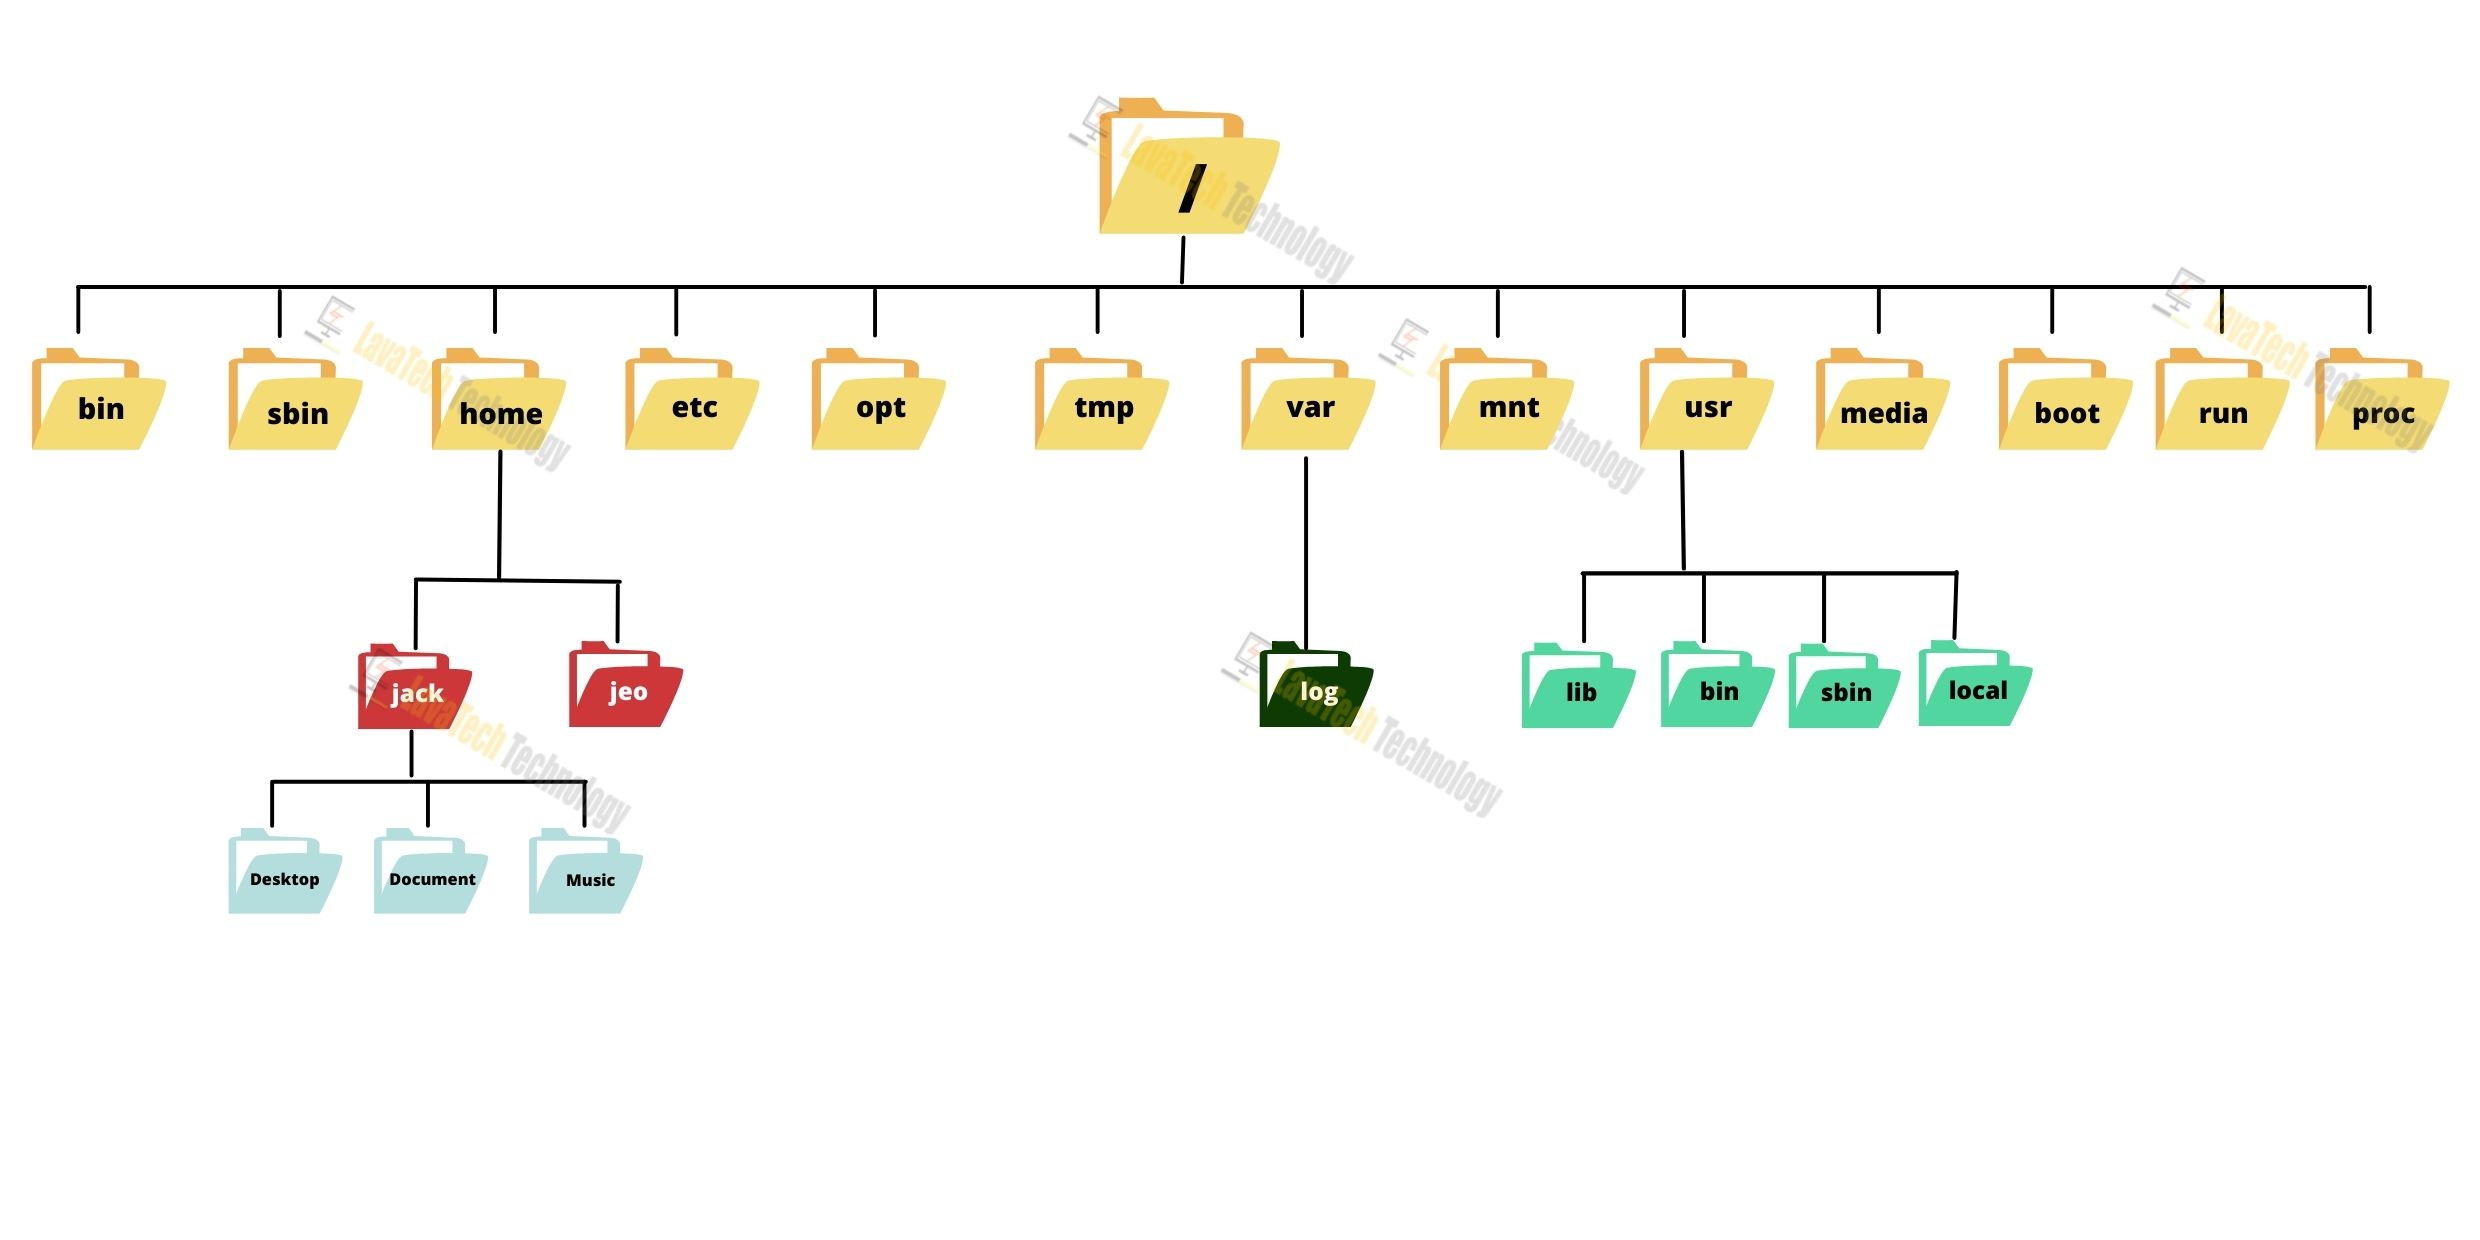
\includegraphics[scale=.24]{content/chapter2/images/fhs.jpg}
		\caption{Filesystem Hierarchy Standard (FHS)}
		\label{fig:fhs}
	\end{figure}
\end{flushleft}

\newpage


\subsection{Important directories in FHS}\index{Linux directory structure!Important Directory You Should Know About}

\begin{flushleft}
	\begin{enumerate}
		\item \textbf{/} 
		\begin{itemize}
			\item "/" is \textbf{top most directory} or \textbf{root directory} or \textbf{starting point} of FHS. 
		\end{itemize}
		\item \textbf{/home}
		\begin{itemize}
			\item Contains \textbf{home folder for each user} having their personal data \& configuration files.
			\item Eg: Home directory for user \textbf{jack} is \textbf{/home/jack}.
			\begin{figure}[h!]
				\centering
				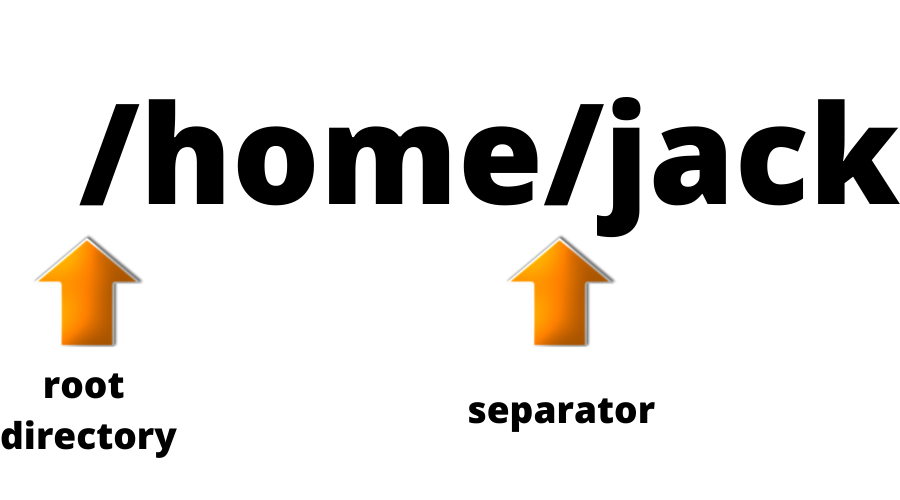
\includegraphics[scale=.3]{content/chapter2/images/path.png}
				\caption{Path separator}
				\label{fig:path}
			\end{figure}
			\begin{tcolorbox}[breakable,notitle,boxrule=-0pt,colback=yellow,colframe=yellow]
				\color{black}
				\textbf{Note:}
				\begin{itemize}
					\item Symbol \textbf{"$\sim$"} refers to the user's home directory.
					\item Eg: If you are logged in as user \textbf{"jack"}, then \textbf{"$\sim$"} meant \textbf{"/home/jack"}.
					\item Eg: If you are logged in as user \textbf{"jill"}, then \textbf{$\sim$} meant \textbf{"/home/jill"}.
					\end{itemize}
			\end{tcolorbox}
			
		\end{itemize}
		\item \textbf{/bin}
		\begin{itemize}
			\item Contains user binaries (programs).
			\item Eg: cp, mkdir, pwd, ls, rmdir etc.
		\end{itemize}
		\item \textbf{/sbin}
		\begin{itemize}
			\item Contains system administration binaries.
			\item Eg: fdisk, useradd, userdel, ifconfig etc.
		\end{itemize}
	\newpage
		\item \textbf{/usr}
		\begin{itemize}
			\item Contains read-only commands, libraries and data.
			\begin{itemize}
				\item \textbf{/bin} is link to \textbf{/usr/bin}
				\item \textbf{/sbin} is link to \textbf{/usr/sbin}
				\item \textbf{/lib} is link to \textbf{/usr/lib}
			\end{itemize}
		\end{itemize}
		\item \textbf{/etc}
		\begin{itemize}
			\item Contains system-wide configuration files.
			\item Eg: 
			\begin{itemize}
				\item /etc/fstab
				\item /etc/sysconfig/network-script/
			\end{itemize}
		\end{itemize}
			\item \textbf{/opt}
			\begin{itemize}
				\item Opt stands for optional.
				\item Used by proprietary 3rd party software to store their settings.
			\end{itemize}
		\item \textbf{/tmp}
		\begin{itemize}
			\item Contains temporary files of system.
			\item Files under this are deleted when system is rebooted.
		\end{itemize}
		\item \textbf{/var}
		\begin{itemize}
			\item Var stands for variable files.
			\item /var includes:
			\begin{itemize}
				\item System log files: \textbf{/var/log}
				\item Packages and database files: \textbf{/var/lib}
				\item Emails: \textbf{/var/mail}
				\item Lock files: \textbf{/var/lock}
				\item Temporary files needed across reboots: \textbf{/var/tmp}
			\end{itemize}
		\end{itemize}
			\item \textbf{/mnt}
		\begin{itemize}
			\item Temporary mount directory.
		\end{itemize}
		\item \textbf{/boot}
		\begin{itemize}
			\item Contains grub2 bootloader, kernel, initramfs etc. needed during system boot up.
		\end{itemize}
		\item \textbf{/media}
		\begin{itemize}
			\item Mounts temporary media device like USB drive.
		\end{itemize}
	\newpage
		\item \textbf{/proc}
		\begin{itemize}
			\item Contains running process informations.
			\item Eg: /proc/\{pid\} directory contains information about the process with that particular process.
		\end{itemize}
		\item \textbf{/run}
		\begin{itemize}
			\item Used for run-time variable data.
			\item Eg: Socket files, Process IDs etc.
			\item Difference between \textbf{/run} \& \textbf{/tmp}:
			\begin{itemize}
				\item Data in \textbf{/run always get deleted at next boot}
				\item Data in /tmp may or may not get deleted at next boot.
			\end{itemize}
		\end{itemize}
	\end{enumerate}
	
\end{flushleft}

\newpage

\subsection{General Linux Shortcuts}
\setlength{\columnsep}{5pt}

\begin{flushleft}
	\paragraph{}
	%\begin{tabulary}{1.0\textwidth}{C|C|C|p{10em}}
	
	\textbf{Useful command line-editing shortcuts}	
	\begin{tabulary}{1.0\textwidth}{|p{10em}|p{18em}|}
		\toprule
		\textbf{Shortcut} & \textbf{Description}\\
		\midrule
		\textbf{Ctrl + l} & Clear the terminal screen. \\
		\hline
		\textbf{Ctrl + a} & Jump to the beginning of the command line. \\
		\hline
		\textbf{Ctrl + e} & Jump to the beginning of the command line. \\
		\hline
		\textbf{Ctrl + u} & Clear from the cursor to the beginning of the command line. \\
		\hline
		\textbf{Ctrl + k} & Clear from the cursor to the end of the command line. \\
		\hline
		\textbf{Ctrl + r} & Search the history list of commands for a pattern. \\
		\hline
		\textbf{Ctrl + Shift + c} & Copy text from terminal. \\
		\hline
		\textbf{Ctrl + Shift + v} & Paste copied text on terminal. \\
		\hline
		\textbf{Ctrl + Shift + t} & Open new terminal. \\
		\hline
		\textbf{Alt + Tab} & Switch between applications. \\
		\bottomrule
	\end{tabulary}

	
	\label{tab:example} % Unique label used for referencing the table in-text
	%\addcontentsline{toc}{table}{Table \ref{tab:example}} % Uncomment to add the table to the table of contents
	
	
	
\end{flushleft}

\newpage
\subsection{Practice}\index{Linux directory structure!Practice}
\setlength{\columnsep}{3pt}
\begin{flushleft}
	\paragraph{}

	\bigskip

	\begin{figure}[h!]
		\centering
		
\includegraphics[scale=.2]{content/practise.jpg}
	\end{figure}	
	
	\begin{enumerate}
		\item \textbf{Does Linux OS have same directory structure as Windows OS?}
		\begin{enumerate}[label=(\alph*)]
			\item Yes
			\item No    %correct
		\end{enumerate}
		\bigskip
		\bigskip
		\item \textbf{Which of the following is the top most directory in Linux OS?}
		\begin{enumerate}[label=(\alph*)]
			\item /         %correct
			\item /home
			\item /root
			\item /boot
		\end{enumerate}
		\bigskip
		\bigskip
		\item \textbf{Which of the following directories contains user binaries \& system administration binaries? }
		\begin{enumerate}[label=(\alph*)]
			\item /bin             %correct
			\item /usr/bin %correct
			\item /usr/sbin %correct
			\item /sbin %correct
		\end{enumerate}
		\bigskip
		\bigskip
		\item \textbf{State whether true or false. All files and directories under /tmp may or may not get deleted on system reboot.}
		\begin{enumerate}[label=(\alph*)]
			\item True          %correct
			\item False
		\end{enumerate}
		\bigskip
		\bigskip
		\item \textbf{Which of the following files/folders are present under /var directory?}
		\begin{enumerate}[label=(\alph*)]
			\item /var/tmp   %correct
			\item /var/log   %correct
			\item /var/mail  %correct
			\item /var/spool  %correct
		\end{enumerate}
		\bigskip
		\bigskip
		\item \textbf{Which of the following directory is used for auto-mounting CD-ROM or USB drive?}
		\begin{enumerate}[label=(\alph*)]
			\item /mnt
			\item /media  %correct
			\item /tmp
			\item /run
		\end{enumerate}
		\bigskip
		\bigskip
		\item \textbf{Which of the following directory stores information about optional third party application like VLC media player.}
		\begin{enumerate}[label=(\alph*)]
			\item /mnt
			\item /media
			\item /opt     %correct
			\item /run
		\end{enumerate}
		\bigskip
		\bigskip
		\item \textbf{The system process in running state stores it's process id and other related information in which of the following directory?}
		\begin{enumerate}[label=(\alph*)]
			\item /mnt
			\item /proc  %correct
			\item /tmp
			\item /run
		\end{enumerate}
			\bigskip
			\bigskip
		\item \textbf{Where is the kernel of Linux OS stored?}
		\begin{enumerate}[label=(\alph*)]
			\item /bin
			\item /usr
			\item /proc
			\item /boot    %correct
		\end{enumerate}  
	\end{enumerate}

	
\end{flushleft}
\newpage



\section{Linux commands}\index{Linux commands}
\setlength{\columnsep}{3pt}
\begin{flushleft}
	\bigskip
	\bigskip
	\begin{tcolorbox}[breakable,notitle,boxrule=1pt,colback=black,colframe=black]
		\color{white}
		\bigskip
		In this section, you are going to learn:
		\begin{enumerate}
			\item \textbf{Basic commands in Linux OS}
			\item \textbf{Advance commands in Linux OS}
		\end{enumerate}	
		\bigskip
		Finally, there will be a \textbf{small excerise} on these topics to check your knowledge.
		\bigskip
	\end{tcolorbox}
	
	
	\bigskip
	\bigskip
	
	\begin{multicols}{2}
		\vspace*{\fill}
		\vspace*{\fill}
		\vspace*{\fill}
		\vspace*{\fill}
		\vspace*{\fill}
		\vspace*{\fill}
		\vspace*{\fill}
		\vspace*{\fill}
		\vspace*{\fill}
		
		\vfill \null
		\columnbreak
		So let's get started....
		
\includegraphics[scale=0.08]{content/linux_section.png}
	\end{multicols}	
	
\end{flushleft}

\newpage






\subsection{Basic commands}\index{Linux commands!Basic commands}


\begin{flushleft}
	Before starting with basic commands, let's first understand a few things.
	\paragraph{What is command prompt?}
	\begin{itemize}
		\item Command prompt is also known as shell prompt.
		\item Commands are entered in a terminal at the shell prompt. 
		\begin{figure}[h!]
			\centering
			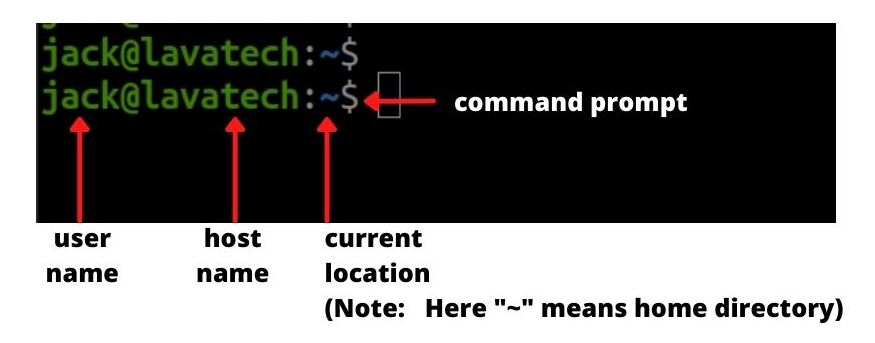
\includegraphics[scale=.5]{content/chapter2/images/command_prompt1.jpg}
			\caption{Command Prompt}
			\label{fig:command_prompt1}
		\end{figure}
		\begin{figure}[h!]
			\centering
			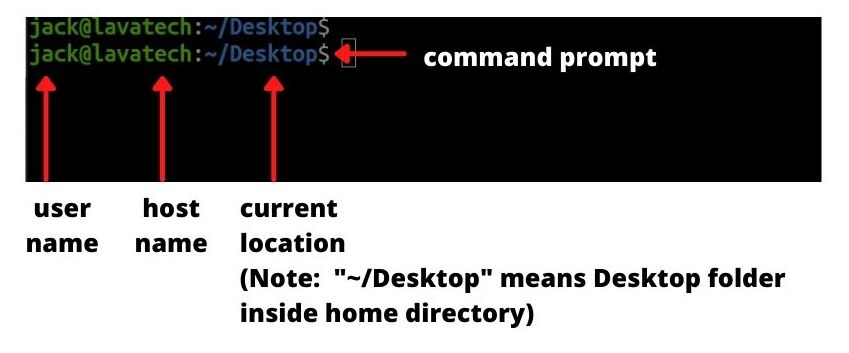
\includegraphics[scale=.5]{content/chapter2/images/command_prompt2.jpg}
			\caption{Command Prompt}
			\label{fig:command_prompt2}
		\end{figure}
		\item The shell prompt lists:
		\begin{itemize}
			\item Username who logged in
			\item Server hostname
			\item Current directory 
			\item \textbf{"\$"} prompt (if you are normal user) or \textbf{"\#"} prompt (if you are root user)
		\end{itemize}		
	

	\end{itemize}
		
	\newpage

	\paragraph{Command syntax}
	
	\begin{itemize}
		\item Commands entered at the shell prompt have three parts:
		\bigskip
			\begin{tcolorbox}[breakable,notitle,boxrule=-0pt,colback=pink,colframe=pink]
			\color{black}
			\fontdimen2\font=1em
			\bigskip
			Syntax:  command [options] [argument]
			\fontdimen2\font=4pt
			\bigskip
		\end{tcolorbox}
		Explaination:
		\begin{itemize}
			\item \textbf{command}: name of command
			\item \textbf{options}: start with one or two dashes (eg: -a or –all)
			\item \textbf{arguments}: a target that the command should operate on
			\item \textbf{"[]"} means optional.
		\end{itemize}

		\item
		Eg:
		\begin{figure}[h!]
			\centering
			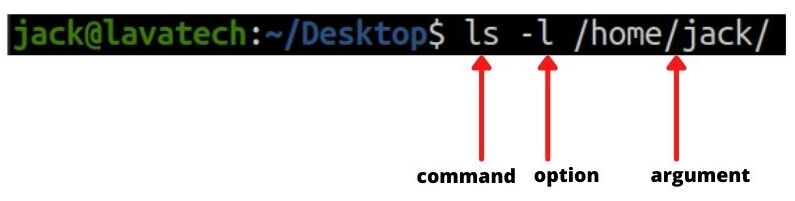
\includegraphics[scale=.65]{content/chapter2/images/command_prompt3.jpg}
			\caption{Command syntax}
			\label{fig:command_prompt3}
		\end{figure}
	\end{itemize}

	\newpage
	\paragraph{Now let's get started with some actual commands.}
	
	\begin{enumerate}
		\item \textbf{pwd}: Shows the user’s present working directory.
		\newline
		Eg:
		\begin{tcolorbox}[breakable,notitle,boxrule=-0pt,colback=black,colframe=black]
			\color{green}
			\fontdimen2\font=1em
			\# pwd
			\fontdimen2\font=4pt
		\end{tcolorbox}
		\bigskip
		\bigskip

		\item \textbf{clear}: Clears the contents of the screen.
		\newline	
		Eg:
		\begin{tcolorbox}[breakable,notitle,boxrule=-0pt,colback=black,colframe=black]
			\color{green}
			\fontdimen2\font=1em
			\# clear
			\fontdimen2\font=4pt
		\end{tcolorbox}
		\bigskip
		\begin{tcolorbox}[breakable,notitle,boxrule=-0pt,colback=orange,colframe=orange]
			\color{black}
			\textbf{Tip:} You can use the keyboard shortcut \textbf{CTRL+L} as well to clear the screen.
		\end{tcolorbox}
	
		\bigskip
		\bigskip
		
		\item \textbf{mkdir}: Create a directory.
		\bigskip
		\begin{tcolorbox}[breakable,notitle,boxrule=1pt,colback=pink,colframe=pink]
			\color{black}
			\fontdimen2\font=1em
			Syntax:  mkdir [options] foldername
			\fontdimen2\font=4pt
		\end{tcolorbox}
		Eg:
		\bigskip
		\begin{tcolorbox}[breakable,notitle,boxrule=-0pt,colback=black,colframe=black]
			\color{green}
			\fontdimen2\font=1em
			\# mkdir /home/jack/test
			\fontdimen2\font=4pt
		\end{tcolorbox}
		Option of \textbf{mkdir} command:
		\begin{itemize}
			\item -p: Creates a directory and all its parents too.
			\newline
			Eg:
			\begin{tcolorbox}[breakable,notitle,boxrule=-0pt,colback=black,colframe=black]
				\color{green}
				\fontdimen2\font=1em
				\# mkdir -p /home/jack/test/a/b/c
				\fontdimen2\font=4pt
			\end{tcolorbox}
		\end{itemize}
		\bigskip

		\item \textbf{ls}: Lists the content of a directory.
		\bigskip
		\begin{tcolorbox}[breakable,notitle,boxrule=1pt,colback=pink,colframe=pink]
			\color{black}
			\fontdimen2\font=1em
			Syntax:  ls [options] [foldername]
			\fontdimen2\font=4pt
		\end{tcolorbox}
	
		Eg:
		\bigskip
		\begin{tcolorbox}[breakable,notitle,boxrule=-0pt,colback=black,colframe=black]
			\fontdimen2\font=1em
			\color{yellow}
            \# List current directory content
            \newline
            \color{green}
			\# ls        
			\newline
			\newline
			\color{yellow}
			\# List content of /home directory
			\newline
			\color{green}
			\# ls /home                
			\fontdimen2\font=4pt
		\end{tcolorbox}
	
		Options with \textbf{ls} command-
		\begin{itemize}		
			\item \textbf{-l}: List more details of contents inside directory.
			\newline
			Eg:
			\begin{tcolorbox}[breakable,notitle,boxrule=-0pt,colback=black,colframe=black]
				\color{green}
				\$ ls -l /home
				\color{white}
				\small
				\fontdimen2\font=1em
				\newline
				total 24
				\newline
				drwxr-xr-x    3    jack   jack    4096 Feb2 17:02 jack
				\newline
				drwx------  2 root   root   16384 Dec8 14:39 lost+found
			\end{tcolorbox}
			Output explaination:
			\begin{itemize}
			\item Column 1 – Type \& permissions of file
				\item Column 2 - Number of links
				\item Column 3 - Owner of the file
				\item Column 4 - Group under which the file belongs
				\item Column 5 - Size of file
				\item Column 6 - Date of last update
				\item Column 7 – Last updated time of file
				\item Column 8 - Name of file/directory
			\end{itemize}
			\item \textbf{-d}: Shows information about directory rather than listing.
			\newline
			Eg:
			\begin{tcolorbox}[breakable,notitle,boxrule=-0pt,colback=black,colframe=black]
				\color{green}
				\# ls -ld 
				\color{white}
				%\small
				\fontdimen2\font=1em
				\newline
				drwxr-xr-x 3 jack jack 4096 Feb  2 17:02 .
				\fontdimen2\font=4pt
			\end{tcolorbox}
		
			\item \textbf{-a}: Shows all files, including hidden files. 
			\bigskip
			\begin{tcolorbox}[breakable,notitle,boxrule=-0pt,colback=yellow,colframe=yellow]
				\color{black}
				Note: Names of hidden files/folders begin with a dot.
			\end{tcolorbox}
			
			Eg:
			\begin{tcolorbox}[breakable,notitle,boxrule=-0pt,colback=black,colframe=black]
				\color{green}
				\fontdimen2\font=1em
				\# ls -a
				\color{white}
				\newline
				.  ..  .bash\_logout  .bashrc  Desktop  .profile
				\fontdimen2\font=4pt
			\end{tcolorbox}
		\end{itemize}
		\bigskip
		\bigskip

		\newpage
		\item \textbf{cd}: Used to switch between directories.
		\bigskip
		\begin{tcolorbox}[breakable,notitle,boxrule=1pt,colback=pink,colframe=pink]
			\color{black}
			\fontdimen2\font=1em
			Syntax:  cd [foldername]
			\fontdimen2\font=4pt
		\end{tcolorbox}
		Eg:
		\begin{tcolorbox}[breakable,notitle,boxrule=-0pt,colback=black,colframe=black]
			\fontdimen2\font=1em
			\color{yellow}
			\# \textbf{cd} without any argument \textbf{switch to user's home directory}.
			\newline
			\color{green}
			\# cd
			\fontdimen2\font=4pt
		\end{tcolorbox}
		Special characters that can be used with "cd" command:
		\begin{itemize}
			\item "." means current directory
			\item ".." means parent directory
			\item "–" would take you to previous working directory
			\item {"$\sim$"} would take you to home directory of the user
		\end{itemize}
		Eg:
		\begin{tcolorbox}[breakable,notitle,boxrule=-0pt,colback=black,colframe=black]
			\color{green}
			\fontdimen2\font=1em
			\# cd /home/
			\newline
			\# cd ..
			\newline
			\# cd -
			\newline
			\# cd {$\sim$}
			\fontdimen2\font=4pt
		\end{tcolorbox}

		\bigskip
		\bigskip
		\textbf{Absolute Path \& Relative Path}: 
		\begin{itemize}
			\item \textbf{Absolute path}: Starts with root directory (i.e "/") \& is complete path. 
			\item \textbf{Relative path}: It is relative to current location \& does not start with root directory (i.e "/").
			\begin{figure}[h!]
				\centering
				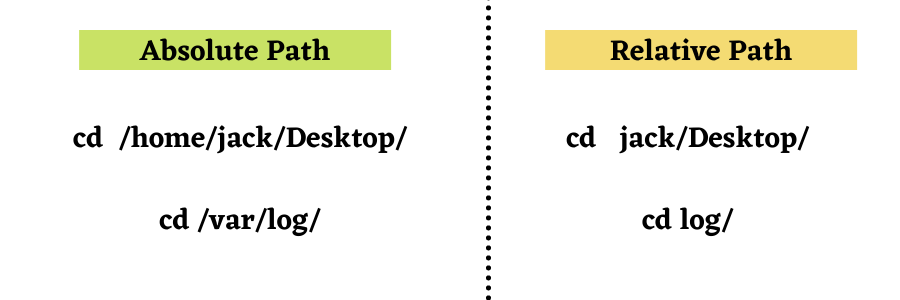
\includegraphics[scale=.45]{content/chapter2/images/path2.png}
				\caption{Absolute \& relative path}
				\label{fig:path2}
			\end{figure}	
		\end{itemize}
	
		\newpage		
		\item \textbf{cat}: Used to display contents of a file and also to create one.
		\begin{enumerate}[label=(\alph*)]
			\item Creating a file:
			\newline
			Eg:
			\begin{tcolorbox}[breakable,notitle,boxrule=-0pt,colback=black,colframe=black]
				\color{green}
				\fontdimen2\font=1em
				\# cat > hello.txt
				\newline
				hi
				\newline
				welcome to unix 
				\newline
				\color{yellow}
				\# End by pressing Ctrl + d
			\fontdimen2\font=4pt
			\end{tcolorbox}
			\item Displaying a file:
			\newline
			Eg:
			\begin{tcolorbox}[breakable,notitle,boxrule=-0pt,colback=black,colframe=black]
				\color{green}
				\fontdimen2\font=1em
				\# cat hello.txt
				\fontdimen2\font=4pt
			\end{tcolorbox}
		\end{enumerate}


		\bigskip
		\bigskip
		\item \textbf{touch}: Performs 2 functions:
		\begin{enumerate}[label=(\alph*)]
		\item Update timestamp of file, if it exists.
		\item Creates a new file, if it does not exists.
		\newline
		Eg:
		\begin{tcolorbox}[breakable,notitle,boxrule=-0pt,colback=black,colframe=black]
			\color{green}
			\fontdimen2\font=1em
			\# touch abc.txt
			\fontdimen2\font=4pt
		\end{tcolorbox}
		\end{enumerate}
		
		You can create multiple files using brace expansion.
		\newline
		Eg:
		\begin{tcolorbox}[breakable,notitle,boxrule=-0pt,colback=black,colframe=black]
			\color{green}
			\fontdimen2\font=1em
			\# touch {Sunday,Monday,Tuesday,Wednesday}.txt
			\newline
			\# touch file{1..3}.txt
			\newline
			\# touch file{a..h}.txt
			\newline
			\# touch file{a,b}{1,2}.txt
			\fontdimen2\font=4pt
		\end{tcolorbox}
		
		\bigskip
		\bigskip
		\item \textbf{cp}: Copy file or directory.
		\bigskip
		\begin{tcolorbox}[breakable,notitle,boxrule=1pt,colback=pink,colframe=pink]
			\color{black}
			\fontdimen2\font=1em
			Syntax: cp source destination
			\fontdimen2\font=4pt
		\end{tcolorbox}
		To copy multiple files to a directory:
			\bigskip
			\begin{tcolorbox}[breakable,notitle,boxrule=-0pt,colback=black,colframe=black]
				\color{green}
				\fontdimen2\font=1em
				\# cp file1 file2 file3 backup
				\fontdimen2\font=4pt
			\end{tcolorbox}

		Options with \textbf{cp} command:
		\begin{enumerate}[label=(\alph*)]
				\item \textbf{-r}: Copy directories recursively including all its files and subdirectories.
				\newline
				Eg:
				\begin{tcolorbox}[breakable,notitle,boxrule=-0pt,colback=black,colframe=black]
					\color{green}
					\fontdimen2\font=1em
					\# cp -r folder1  newfolder
					\fontdimen2\font=4pt
			\end{tcolorbox}
			\item \textbf{Wildcard character "*"}: Copy all files starting with a specific name.
			\bigskip
			\begin{tcolorbox}[breakable,notitle,boxrule=-0pt,colback=black,colframe=black]
				\color{green}
				\fontdimen2\font=1em
				\# cp file* backup
				\fontdimen2\font=4pt
			\end{tcolorbox}
		\end{enumerate}
		\bigskip
		\bigskip		

		
		\item \textbf{mv}: Used to move or rename the file/folder.
		\bigskip
		\begin{tcolorbox}[breakable,notitle,boxrule=1pt,colback=pink,colframe=pink]
			\color{black}
			\fontdimen2\font=1em
			Syntax:  mv source destination
			\fontdimen2\font=4pt
		\end{tcolorbox}
		\begin{enumerate}[label=(\alph*)]
		\item Renames file(or directory) when the \textbf{location of source and destination is same.}
		\bigskip
		\begin{tcolorbox}[breakable,notitle,boxrule=1pt,colback=black,colframe=black]
			\color{green}
			\fontdimen2\font=1em
			\# mv old-file new-file
			\fontdimen2\font=4pt
		\end{tcolorbox}
		\item Moves a files/directory to different location if \textbf{source and destination is different.}
		\bigskip
		\begin{tcolorbox}[breakable,notitle,boxrule=-0pt,colback=black,colframe=black]
			\color{green}
			\fontdimen2\font=1em
			\# mv oldfile new-file-location
			\fontdimen2\font=4pt
		\end{tcolorbox}
		\end{enumerate}
		\bigskip
		\bigskip
	
		\item \textbf{rm}: Deletes one or more files/folders.
		\bigskip
		\begin{tcolorbox}[breakable,notitle,boxrule=1pt,colback=pink,colframe=pink]
			\color{black}
			\fontdimen2\font=1em
			Syntax:  rm filename
			\fontdimen2\font=4pt
		\end{tcolorbox}
		Eg:
		\begin{tcolorbox}[breakable,notitle,boxrule=-0pt,colback=black,colframe=black]
			\color{green}
			\fontdimen2\font=1em
			\# rm one.txt
			\fontdimen2\font=4pt
		\end{tcolorbox}
		Options with \textbf{rm} command:
		\begin{enumerate}[label=(\alph*)]
			\item \textbf{-r}: Remove directories and their contents recursively.
			\bigskip
			\begin{tcolorbox}[breakable,notitle,boxrule=-0pt,colback=black,colframe=black]
				\color{green}
				\fontdimen2\font=1em
				\# rm -r foldername
				\fontdimen2\font=4pt
			\end{tcolorbox}
		\end{enumerate}	
		\bigskip
		\bigskip
		\newpage
		\item \textbf{rmdir}: Deletes only empty directory.
		\bigskip
		\begin{tcolorbox}[breakable,notitle,boxrule=1pt,colback=pink,colframe=pink]
			\color{black}
			\fontdimen2\font=1em
			Syntax:  rmdir directory
			\fontdimen2\font=4pt
		\end{tcolorbox}
		Eg:
		\begin{tcolorbox}[breakable,notitle,boxrule=-0pt,colback=black,colframe=black]
			\color{green}
			\fontdimen2\font=1em
			\# rmdir /tmp/project/
			\fontdimen2\font=4pt
		\end{tcolorbox}
		\bigskip
		\bigskip
		\item \textbf{df}: df stands for \textbf{disk free}. Displays information about disk usage.
		\bigskip
		\begin{tcolorbox}[breakable,notitle,boxrule=1pt,colback=pink,colframe=pink]
			\color{black}
			\fontdimen2\font=1em
			Syntax:  df
			\fontdimen2\font=4pt
		\end{tcolorbox}
		Options with \textbf{df} command:
		\begin{enumerate}[label=(\alph*)]
			\item \textbf{-h}: Display disk-usage size in GBs, MBs etc.
			\newline
			Eg:
			\begin{tcolorbox}[breakable,notitle,boxrule=1pt,colback=black,colframe=black]
				\color{green}
				\fontdimen2\font=1em
				\# df -h
				\fontdimen2\font=4pt
			\end{tcolorbox}
			\item \textbf{-T}: Print filesystem of each partition.
			\newline
			Eg:
			\begin{tcolorbox}[breakable,notitle,boxrule=-0pt,colback=black,colframe=black]
				\color{green}
				\fontdimen2\font=1em
				\# df -T
				\fontdimen2\font=4pt
			\end{tcolorbox}
		\end{enumerate}	
		\bigskip
		\bigskip
		
		\end{enumerate}
\end{flushleft}

\newpage


\subsection{Advance commands}\index{Linux commands!Advance commands}

\begin{flushleft}
	
	\begin{enumerate}
		\item \textbf{whoami}: Display username who is logged in.
		\newline
		Eg:
		\begin{tcolorbox}[breakable,notitle,boxrule=-0pt,colback=black,colframe=black]
			\color{green}
			\# whoami
			\newline
			\color{white}
			jack
		\end{tcolorbox}
		\bigskip
		\bigskip
		
		\item \textbf{users}: Display all the username who are currently logged in.
		\newline
		Eg:
		\begin{tcolorbox}[breakable,notitle,boxrule=-0pt,colback=black,colframe=black]
			\color{green}
			\# users
			\newline
			\fontdimen2\font=1em
			\color{white}
			jack jill lavatech
			\fontdimen2\font=4pt
		\end{tcolorbox}
		
		\bigskip
		
		\item \textbf{who}: Displays users currently logged with more details.
		\newline
		Eg:
		\begin{tcolorbox}[breakable,notitle,boxrule=-0pt,colback=black,colframe=black]
			\color{green}
			\# who
			\newline
			\color{white}
			\fontdimen2\font=1em
			jack   :0           2022-02-02 14:21 (:0)
			\newline
			jill :1           2022-02-03 13:52 (:1)
			\newline
			lavatech pts/0  2022-02-03 14:03 (192.168.0.105)
			\fontdimen2\font=4pt
		\end{tcolorbox}				
		Output explaination:
			\begin{itemize}
				\item Column 1 - Login name
				\item Column 2 - Login device (TTY or pts)
				\item Column 3 - Login date
				\item Column 4 - Login time 
				\item Column 5 - Local device or remote IP address from where the user is logged in
			\end{itemize}
		\bigskip
		\begin{tcolorbox}[breakable,notitle,boxrule=-0pt,colback=yellow,colframe=yellow]
			\color{black}
			\textbf{Note:} 
			\begin{itemize}
				\item TTY stands for \textbf{teletypewriter}: It is an input device that allows alphanumeric character to be typed in and sent to a computer.
				\item The pts/0 is telling which \textbf{"pseudo terminal"} the user is logged in on. 
			\end{itemize}
		\end{tcolorbox}
		Options with \textbf{who} command:
		\begin{itemize}
			\item \textbf{-H}: Prints the column headers.
			\newline
			Eg:
			\begin{tcolorbox}[breakable,notitle,boxrule=-0pt,colback=black,colframe=black]
				\color{green}
				\$ who -H 
			\end{tcolorbox}
			\item \textbf{-b}: Display the time and date of the last reboot.
			\newline
			Eg:
			\begin{tcolorbox}[breakable,notitle,boxrule=-0pt,colback=black,colframe=black]
				\color{green}
				\# who -b
			\end{tcolorbox}
		\end{itemize}
		\bigskip
		\item \textbf{w}: Shows who is logged and what they are doing.
			\newline
			Eg:
			\begin{tcolorbox}[breakable,notitle,boxrule=-0pt,colback=black,colframe=black]
				\color{green}
				\# w
				\color{white}
				\small
				\fontdimen2\font=1em
				\newline
				14:27:00 up 1 day, 5 min,  2 users,  load average: 1.86, 2.44, 2.70
				\newline
				\fontdimen2\font=1.2em
				USER     TTY      FROM             LOGIN@   IDLE   JCPU   PCPU WHAT
				\newline
				jack   :0       :0               Wed14   ?xdm?  14:25m  0.03s /usr/lib/g
				\newline
				lavatech :1       :1               13:52   ?xdm?  14:25m  0.00s /usr/lib/g
				\newline
				\fontdimen2\font=4pt
			\end{tcolorbox}
			
			Output explaination:
			\begin{itemize}
				\item Line 1 - Shows below details:
				\begin{itemize}
					\item Current time
					\item How long the system has been running.
					\item How many users are currently logged in.
					\item System load averages for the past 1, 5, and 15 minutes.
				\end{itemize}
				\item Line 2 - Header
				\item Line 3 - Login name, the tty name, the remote host, login time, idle time, JCPU, PCPU, and the command line of their current process.
			\end{itemize}
			\bigskip
			\bigskip
			\textbf{JCPU} - Time used by all processes attached to the tty.
			\newline
			\textbf{PCPU} - Time used by the current process, named in the "what" field.
		\bigskip
		\item \textbf{uname}: Displays the name of OS.
		\newline
		Eg:
		\begin{tcolorbox}[breakable,notitle,boxrule=-0pt,colback=black,colframe=black]
			\color{green}
			\fontdimen2\font=1em
			\# uname
			\newline
			\color{white}
			Linux
			\fontdimen2\font=4pt
		\end{tcolorbox}
		Options with \textbf{uname} command:
		\begin{itemize}
			\item \textbf{-r}: Displays the current release of OS.
			\newline
			Eg:
			\begin{tcolorbox}[breakable,notitle,boxrule=-0pt,colback=black,colframe=black]
				\color{green}
				\fontdimen2\font=1em
				\# uname -r
				\color{white}
				\newline
				3.6.18-194.el8
				\fontdimen2\font=4pt
			\end{tcolorbox}
			\item \textbf{-a}: Displays:
			\begin{itemize}
				\item Kernel name 
				\item System name 
				\item Kernel release
				\item Kernel version
				\item Machine processor 
				\item Hardware platform
			\end{itemize} 
			Eg:
			\begin{tcolorbox}[breakable,notitle,boxrule=-0pt,colback=black,colframe=black]
				\color{green}
				\fontdimen2\font=1em
				\# uname -a
				\color{white}
				\newline
				Linux lavatech 5.13.0-27-generic \#29~20.04.1-Ubuntu SMP Fri Jan 14 00:32:30 UTC 2022 x86\_64 x86\_64 x86\_64 GNU/Linux
				\fontdimen2\font=4pt
			\end{tcolorbox}
			\item \textbf{-n}: Prints the hostname of machine.
			\newline
			Eg:
			\begin{tcolorbox}[breakable,notitle,boxrule=-0pt,colback=black,colframe=black]
				\color{green}
				\fontdimen2\font=1em
				\# uname -n
				\fontdimen2\font=4pt
			\end{tcolorbox}
		\end{itemize}
		\bigskip
		
		\item \textbf{uptime}: Display belows details in one line:
		\begin{itemize}
			\item Current time
			\item How long the system has been running
			\item How many users are currently logged in
			\item System load averages for the past 1, 5, and 15 minutes
		\end{itemize}
		Eg:
		\begin{tcolorbox}[breakable,notitle,boxrule=-0pt,colback=black,colframe=black]
			\color{green}
			\fontdimen2\font=1em
			\# uptime
			\newline
			\color{white}
			 14:48:33 up 1 day, 27 min,  2 users,  load average: 2.58, 2.60, 2.76
			\fontdimen2\font=4pt
		\end{tcolorbox}
		\bigskip
		\bigskip
		\item \textbf{timedatectl}: Control the system time and date
		\bigskip
		\begin{tcolorbox}[breakable,notitle,boxrule=-0pt,colback=pink,colframe=pink]
			\color{black}
			\fontdimen2\font=1em
			Syntax: timedatectl [options] [arguments]
			\fontdimen2\font=4pt
		\end{tcolorbox}
		Eg:
		\begin{figure}[h!]
			\centering
			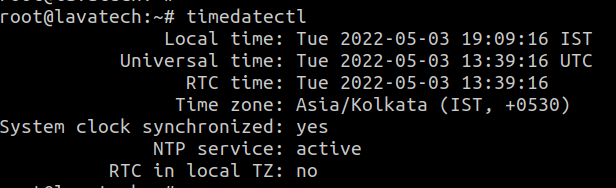
\includegraphics[scale=.45]{content/chapter2/images/timedate.png}
			\caption{Sample output}
			\label{fig:path25}
		\end{figure}
		\newline	
		Options with \textbf{timedatectl} command:
		\begin{itemize}
			\item \textbf{list-timezones}: Displays all available timezones.
			\newline
			Eg:
			\begin{tcolorbox}[breakable,notitle,boxrule=-0pt,colback=black,colframe=black]
				\color{green}
				\fontdimen2\font=1em
				\# timedatectl list-timezones
				\fontdimen2\font=4pt
			\end{tcolorbox}
			\item \textbf{set-timezone}: Sets timezone.
			\newline
			Eg:
			\begin{tcolorbox}[breakable,notitle,boxrule=-0pt,colback=black,colframe=black]
				\color{green}
				\fontdimen2\font=1em
				\# timedatectl set-timezone America/Jamaica
				\fontdimen2\font=4pt
			\end{tcolorbox}
		\end{itemize}	
		\bigskip
		\bigskip
		\item \textbf{date}: Display or set the date.
		\begin{enumerate}[label=(\alph*)]
			\item To display the date:
			\newline
			Eg:
			\begin{tcolorbox}[breakable,notitle,boxrule=-0pt,colback=black,colframe=black]
				\color{green}
				\fontdimen2\font=1em
				\# date
				\newline
				\color{white}
				Saturday 30 April 2022 12:24:24 PM IST
				\fontdimen2\font=4pt
			\end{tcolorbox}
			\item To set the date, the format is:
			\bigskip
			\begin{tcolorbox}[breakable,notitle,boxrule=1pt,colback=pink,colframe=pink]
				\color{black}
				\fontdimen2\font=1em
				Syntax: date "+\%formatters"
				\fontdimen2\font=4pt
			\end{tcolorbox}
			Eg:
			\bigskip
			\begin{tcolorbox}[breakable,notitle,boxrule=-0pt,colback=black,colframe=black]
				\color{green}
				\fontdimen2\font=1em
				\# date '+\%a \%h \%d \%T'
				\fontdimen2\font=4pt
			\end{tcolorbox}
		
			Valid date formatters:
			\newline
			\newline
			\begin{tabulary}{1.0\textwidth}{|p{8em}|p{16em}|}
				\toprule
				\textbf{Date Formatter} & \textbf{Description}\\
				\midrule
				\%m & month of year (01-12) \\
				\hline
				\%n & prints output to new line \\
				\hline
				\%d & day of month (01-31) \\
				\hline
				\%y & last two digits of year (00-99) \\
				\hline
				\%D & date as mm/dd/yy \\
				\hline
				\%H & hour (00-23) \\
				\hline
				\%M & minute (00-59) \\
				\hline
				\%S & second (00-59) \\
				\hline
				\%T & time as HH:MM:SS \\
				\hline
				\%j & day of year (001-366) \\
				\hline
				\%w & day of week (0-6) Sunday is 0 \\
				\hline
				\%a & abbreviated weekday (Sun-Sat) \\
				\hline
				\%h & abbreviated month (Jan-Dec) \\
				\hline
				\%r & 12-hour time w/ AM/PM (e.g., "03:59:42 PM")\\
				\bottomrule
			\end{tabulary}
		
			Options with \textbf{date} command:
			
			\begin{itemize}
				\item \textbf{-s datestring}: Sets the time and date to the value specified in the datestring only if you are root user.
				\newline
				Eg:
				\bigskip
				\begin{tcolorbox}[breakable,notitle,boxrule=-0pt,colback=black,colframe=black]
					\color{green}
					\fontdimen2\font=1em
					\# date -s '11/20/2003 12:48:00'
					\fontdimen2\font=4pt
				\end{tcolorbox}
				\item \textbf{-d datestring}: Display the specified date instead of actual current system date.
				\newline
				Eg:
				\bigskip
				\begin{tcolorbox}[breakable,notitle,boxrule=-0pt,colback=black,colframe=black]
					\color{green}
					\fontdimen2\font=1em
					\# date -d "last friday"
					\newline
					\# date -d "next friday"
					\newline
					\# date -d "yesterday"
					\fontdimen2\font=4pt
				\end{tcolorbox}
			\end{itemize}
			
		\end{enumerate}
		\bigskip
		\bigskip
		\item \textbf{cal}: Prints a calendar for the current month.
			\bigskip
			\begin{tcolorbox}[breakable,notitle,boxrule=-0pt,colback=pink,colframe=pink]
				\color{black}
				\fontdimen2\font=1em
				Syntax: cal [options] [[month] year]
				\fontdimen2\font=4pt
			\end{tcolorbox}
			Options with \textbf{cal} command:
			\begin{itemize}
				\item \textbf{-j}: Display julian dates (days numbered 1 to 365, starting from January 1).
				\newline
				Eg: To display calender for month-12 and year-2022 with julian dates.
				\begin{tcolorbox}[breakable,notitle,boxrule=-0pt,colback=black,colframe=black]
					\color{green}
					\fontdimen2\font=1em
					\# cal -j 12 2022
					\fontdimen2\font=4pt
				\end{tcolorbox}
				
				\begin{figure}[h!]
					\centering
					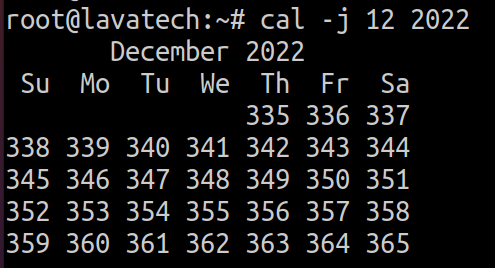
\includegraphics[scale=0.4]{content/chapter2/images/cal1.png}
					\caption{Sample output}
					\label{fig:cal1}
				\end{figure}

				\item \textbf{-m}: Display specific month.
				\newline
				Eg: To display calender of month-12.
				\begin{tcolorbox}[breakable,notitle,boxrule=-0pt,colback=black,colframe=black]
					\color{green}
					\fontdimen2\font=1em
					\# cal -m 12
					\fontdimen2\font=4pt
				\end{tcolorbox}
				
				\begin{figure}[h!]
					\centering
					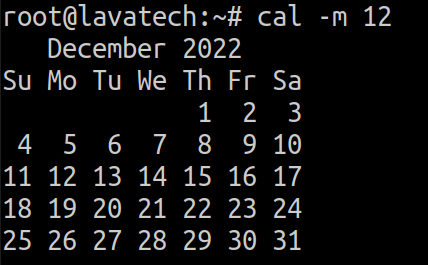
\includegraphics[scale=0.4]{content/chapter2/images/cal2.png}
					\caption{Sample output}
					\label{fig:cal2}
				\end{figure}
				
			
				\item \textbf{-y}: Display entire year.\newline
				Eg: To display calender of year-2022.
			\begin{tcolorbox}[breakable,notitle,boxrule=-0pt,colback=black,colframe=black]
				\color{green}
				\fontdimen2\font=1em
				\# cal -y 2022
				\fontdimen2\font=4pt
			\end{tcolorbox}
			\begin{figure}[h!]
				\centering
				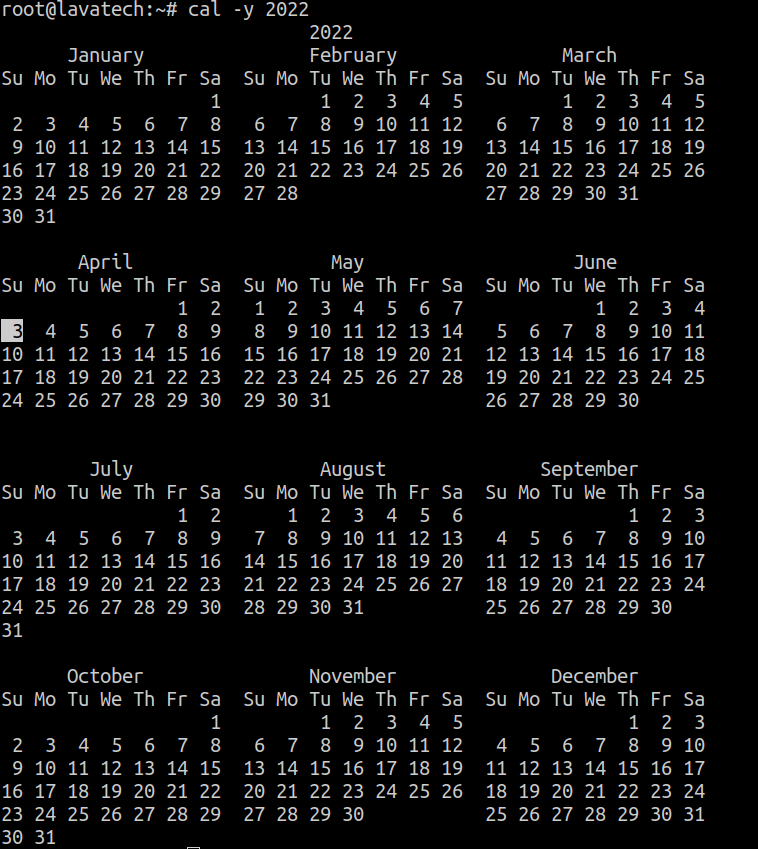
\includegraphics[scale=0.4]{content/chapter2/images/cal3.png}
				\caption{Sample output}
				\label{fig:cal3}
			\end{figure}
			
			\end{itemize}

	\newpage
		\item \textbf{ifconfig}: Display the IP address of server.
		\newline
		Eg:
		\begin{tcolorbox}[breakable,notitle,boxrule=1pt,colback=black,colframe=black]
			\color{green}
			\fontdimen2\font=1em
			\# ifconfig
			\fontdimen2\font=4pt
		\end{tcolorbox}
			\bigskip
			\bigskip		
		\newpage
		\item \textbf{hostname}: Displays the fully qualified name of server.
		\newline
		Eg:
		\begin{tcolorbox}[breakable,notitle,boxrule=1pt,colback=black,colframe=black]
			\color{green}
			\fontdimen2\font=1em
			\# hostname
			\fontdimen2\font=4pt
		\end{tcolorbox}
		\bigskip
		\bigskip
		
		\item \textbf{free}: Displays amount of free and used memory in the system in bytes.
		\newline
			Options with \textbf{free} command:
			\begin{itemize}
				\item \textbf{-k}: Show the output in Kilobytes
				\item \textbf{-m}: Show the output in Megabytes
				\item \textbf{-g}: Show the output in Gegabytes
			\end{itemize}
		Eg:
		\begin{tcolorbox}[breakable,notitle,boxrule=1pt,colback=black,colframe=black]
			\color{green}
			\fontdimen2\font=1em
			\# free 
			\newline
			\# free -k
			\newline
			\# free -m
			\newline
			\# free -g
			\fontdimen2\font=4pt
		\end{tcolorbox}
		
		
		\bigskip
		\bigskip
		\item \textbf{shutdown}: Shutdown the machine immediately or schedule a shutdown using 24 hour format.
		\bigskip
		\begin{tcolorbox}[breakable,notitle,boxrule=1pt,colback=pink,colframe=pink]
			\color{black}
			\fontdimen2\font=1em
			Syntax:  shutdown [options] [time in 24 hour format]
			\fontdimen2\font=4pt
		\end{tcolorbox}
		\bigskip
		\begin{itemize}
			\item Eg: Shutdown immediately -
			\begin{tcolorbox}[breakable,notitle,boxrule=1pt,colback=black,colframe=black]
				\color{green}
				\fontdimen2\font=1em
				\# shutdown -h now
				\newline
				or
				\newline
				\# poweroff
				\fontdimen2\font=4pt
			\end{tcolorbox}
			\item Eg: Reboot the system immediately -
			\bigskip
			\begin{tcolorbox}[breakable,notitle,boxrule=1pt,colback=black,colframe=black]
				\color{green}
				\fontdimen2\font=1em
				\# shutdown -r now
				\newline
				\color{green}
				or
				\newline
				\color{green}
				\# reboot
				\fontdimen2\font=4pt
			\end{tcolorbox}
			\item Eg: Restart OS at specific time, like at 5:30 pm -
			\bigskip
			\begin{tcolorbox}[breakable,notitle,boxrule=1pt,colback=black,colframe=black]
				\color{green}
				\fontdimen2\font=1em
				\# shutdown 17:30
				\fontdimen2\font=4pt
			\end{tcolorbox}
			\item Eg: Shutdown OS at specific time, like at 5:30 pm -
			\bigskip
			\begin{tcolorbox}[breakable,notitle,boxrule=1pt,colback=black,colframe=black]
				\color{green}
				\fontdimen2\font=1em
				\# shutdown -h 17:30
				\fontdimen2\font=4pt
			\end{tcolorbox}
		\end{itemize}

		\bigskip
		\bigskip
		

		\item \textbf{which}: Shows the full path of the command.
		\bigskip
		\begin{tcolorbox}[breakable,notitle,boxrule=1pt,colback=pink,colframe=pink]
			\color{black}
			\fontdimen2\font=1em
			Syntax: which command\_name
			\fontdimen2\font=4pt
		\end{tcolorbox}
		Eg:
		\bigskip
		\begin{tcolorbox}[breakable,notitle,boxrule=1pt,colback=black,colframe=black]
			\color{green}
			\fontdimen2\font=1em
			\# which cal
			\newline
			\color{white}
			/usr/bin/cal
			\fontdimen2\font=4pt
		\end{tcolorbox}

		
		\bigskip
		\bigskip
		
		\item \textbf{whereis}: Locate the binary, source, and manual page files for a command.
		\bigskip
		\begin{tcolorbox}[breakable,notitle,boxrule=1pt,colback=pink,colframe=pink]
			\color{black}
			\fontdimen2\font=1em
			Syntax: whereis command\_name
			\fontdimen2\font=4pt
		\end{tcolorbox}
		Eg:
		\bigskip
		\begin{tcolorbox}[breakable,notitle,boxrule=1pt,colback=black,colframe=black]
			\color{green}
			\fontdimen2\font=1em
			\# whereis cal
			\newline
			\color{white}
			cal: /usr/bin/cal /usr/share/man/man1/cal.1.gz
			\fontdimen2\font=4pt
		\end{tcolorbox}
		\bigskip
		\bigskip
		

		\item \textbf{sleep}: Suspends the shell by making it inactive for specified seconds.
		\begin{tcolorbox}[breakable,notitle,boxrule=1pt,colback=pink,colframe=pink]
			\color{black}
			\fontdimen2\font=1em
			Syntax: sleep seconds
			\fontdimen2\font=4pt
		\end{tcolorbox}
		Eg:
		\bigskip
		\begin{tcolorbox}[breakable,notitle,boxrule=1pt,colback=black,colframe=black]
			\color{green}
			\fontdimen2\font=1em
			\# sleep 10
			\fontdimen2\font=4pt
		\end{tcolorbox}
		\bigskip
		\bigskip	

				
		\item \textbf{history}: Shows last few commands fired by the current user.
		\newline
		Eg:
		\begin{figure}[h!]
			\centering
			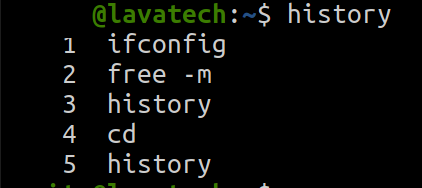
\includegraphics[scale=.4]{content/chapter2/images/history.png}
			\caption{history command output}
			\label{fig:h6}
		\end{figure}
	\newline
		Options using \textbf{history} command:
		\newline
		\textbf{-c}: Clear the history.
			\begin{tcolorbox}[breakable,notitle,boxrule=1pt,colback=pink,colframe=pink]
				\color{black}
				\fontdimen2\font=1em
				Syntax:  history -c
				\fontdimen2\font=4pt
			\end{tcolorbox}
		Shortcuts using \textbf{history} command:
		\newline
		\textbf{!}: Used to repeat the command executed in past, using it's history number.
		\begin{tcolorbox}[breakable,notitle,boxrule=1pt,colback=pink,colframe=pink]
			\color{black}
			\fontdimen2\font=1em
			Syntax:  !history-no
			\fontdimen2\font=4pt
		\end{tcolorbox}
		Eg:
		\begin{figure}[h!]
			\centering
			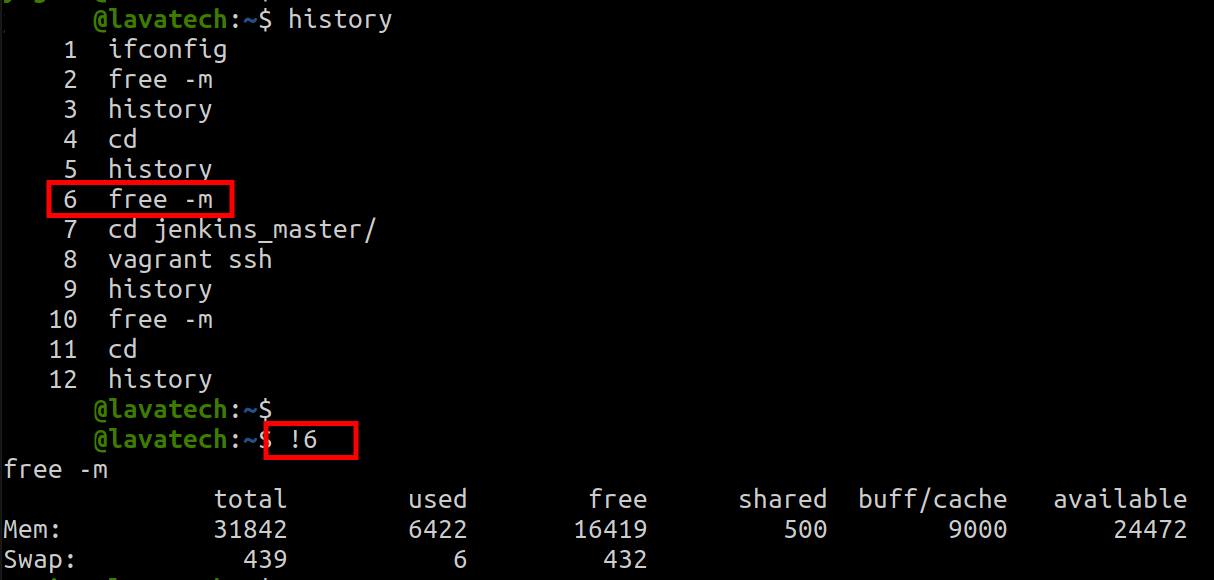
\includegraphics[scale=.2]{content/chapter2/images/history2.png}
			\caption{history command output}
			\label{fig:h88}
		\end{figure}

		\newpage
		\item \textbf{ping}: Used to check if a machine is reachable or not on the network.
		\newline
		\begin{tcolorbox}[breakable,notitle,boxrule=1pt,colback=pink,colframe=pink]
			\color{black}
			\fontdimen2\font=1em
			Syntax:  ping ip-address/hostname
			\fontdimen2\font=4pt
		\end{tcolorbox}
		Eg:
		\begin{tcolorbox}[breakable,notitle,boxrule=1pt,colback=black,colframe=black]
			\color{green}
			\fontdimen2\font=1em
			\# ping 192.168.1.0
			\newline
			\# ping www.google.com
			\fontdimen2\font=4pt
		\end{tcolorbox}
		\bigskip
		\begin{tcolorbox}[breakable,notitle,boxrule=1pt,colback=yellow,colframe=yellow]
			\color{black}
			Note: Ping works continuously until ctrl+c is pressed.
		\end{tcolorbox}
		\bigskip
		Options with \textbf{ping} command:
		\newline
		\textbf{-cN}: Send data N number of times using ping command.	
		\newline
		Eg:
		\begin{figure}[h!]
			\centering
			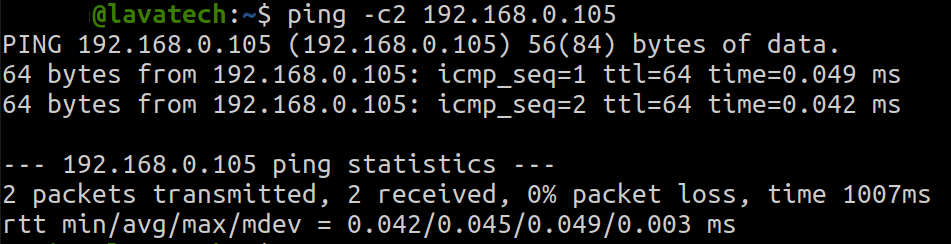
\includegraphics[scale=.35]{content/chapter2/images/ping.png}
			\caption{ping command output}
			\label{fig:h1}
		\end{figure}
		\bigskip
		\bigskip
		\item \textbf{man}: Display manual pages of commands.
		\bigskip
		\begin{tcolorbox}[breakable,notitle,boxrule=1pt,colback=pink,colframe=pink]
			\color{black}
			\fontdimen2\font=1em
			Syntax: man command\_name
			\fontdimen2\font=4pt
		\end{tcolorbox}
		Eg:
		\bigskip
		\begin{tcolorbox}[breakable,notitle,boxrule=1pt,colback=black,colframe=black]
			\color{green}
			\fontdimen2\font=1em
			\# man date
			\fontdimen2\font=4pt
		\end{tcolorbox}
		Options with \textbf{man} command:
		\newline
		\textbf{-k}: Search for man page using keyword
		\begin{tcolorbox}[breakable,notitle,boxrule=1pt,colback=pink,colframe=pink]
			\color{black}
			\fontdimen2\font=1em
			Syntax: man -k keyword
			\fontdimen2\font=4pt
		\end{tcolorbox}
		Eg:
		\begin{figure}[h!]
			\centering
			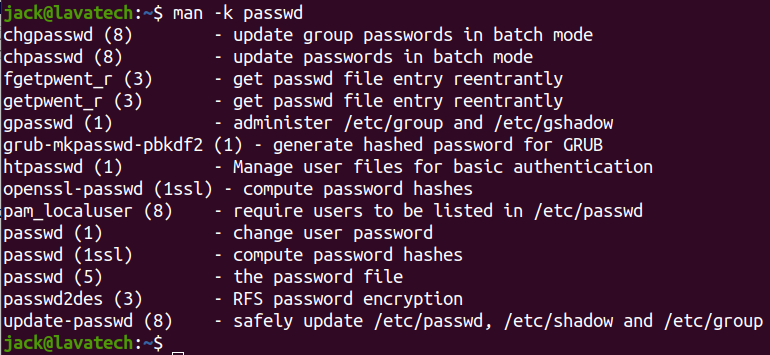
\includegraphics[scale=.5]{content/chapter2/images/man2.png}
			\caption{Command Prompt}
			\label{fig:command_prompt2}
		\end{figure}

	
		\bigskip
		\bigskip


		\item \textbf{whatis}: Provides very brief descriptions of the command.
		\bigskip
		\begin{tcolorbox}[breakable,notitle,boxrule=1pt,colback=pink,colframe=pink]
			\fontdimen2\font=1em
			\color{black}
			Syntax: whatis command\_name
			\fontdimen2\font=4pt
		\end{tcolorbox}
		Eg:
		\bigskip
		\begin{tcolorbox}[breakable,notitle,boxrule=1pt,colback=black,colframe=black]
			\fontdimen2\font=1em
			\color{green}
			\# whatis cal
			\color{white}
			\newline
			cal (1)              - displays a calendar and the date of Easter
			\fontdimen2\font=4pt
		\end{tcolorbox}
		
		\bigskip
		\bigskip
		
		\item \textbf{echo}: Display custom message.
		\bigskip
		\begin{tcolorbox}[breakable,notitle,boxrule=1pt,colback=pink,colframe=pink]
			\color{black}
			\fontdimen2\font=1em
			Syntax: echo "message"
			\fontdimen2\font=4pt
		\end{tcolorbox}
		Eg:
		\bigskip		
		\begin{tcolorbox}[breakable,notitle,boxrule=1pt,colback=black,colframe=black]
			\color{green}
			\fontdimen2\font=1em
			\# echo "lavatech technology training institute"
			\fontdimen2\font=4pt
		\end{tcolorbox}
		Executing command along with custom message:
		\begin{tcolorbox}[breakable,notitle,boxrule=1pt,colback=pink,colframe=pink]
			\color{black}
			\fontdimen2\font=1em
			Syntax: echo "message \$(command)"
			\newline
			or
			\newline
			Syntax: echo "message `command`"
			\fontdimen2\font=4pt
		\end{tcolorbox}
		Eg:
		\bigskip		
		\begin{tcolorbox}[breakable,notitle,boxrule=1pt,colback=black,colframe=black]
			\color{green}
			\fontdimen2\font=1em
			\# echo "lavatech technology training institute, date: \$(date)"
			\newline
			\# echo "lavatech technology training institute, date: `date`"
			\fontdimen2\font=4pt
		\end{tcolorbox}
		\bigskip
		\bigskip	
		
		\item \textbf{alias}: Sets an alias (similar to nickname) for a command.
		\bigskip
		\begin{tcolorbox}[breakable,notitle,boxrule=1pt,colback=pink,colframe=pink]
			\color{black}
			\fontdimen2\font=1em
			Syntax: alias 'shortcutname=command'
			\fontdimen2\font=4pt
		\end{tcolorbox}
		Eg:
		\bigskip
		\begin{tcolorbox}[breakable,notitle,boxrule=1pt,colback=black,colframe=black]
			\color{green}
			\fontdimen2\font=1em
			\# alias 'cls=clear'           
			\fontdimen2\font=4pt
		\end{tcolorbox}
		\bigskip
		\bigskip	
		
		\item \textbf{unalias}: Remove an alias.
		\bigskip
		\begin{tcolorbox}[breakable,notitle,boxrule=1pt,colback=pink,colframe=pink]
			\color{black}
			\fontdimen2\font=1em
			Syntax: unalias shortcutname
			\fontdimen2\font=4pt
		\end{tcolorbox}
		Eg:
		\bigskip
		\begin{tcolorbox}[breakable,notitle,boxrule=1pt,colback=black,colframe=black]
			\color{green}
			\fontdimen2\font=1em
			\# unalias cls
			\fontdimen2\font=4pt
		\end{tcolorbox}
		\bigskip
		\bigskip	
		

		
	\end{enumerate}
	
\end{flushleft}

\newpage


\subsection{Practice}\index{Linux commands!Practice}
\setlength{\columnsep}{3pt}
\begin{flushleft}
	\paragraph{}
	
	\bigskip
	
	\begin{figure}[h!]
		\centering
		
\includegraphics[scale=.2]{content/practise.jpg}
	\end{figure}	
	
	\begin{enumerate}
		\item \textbf{Which of the following command is used to list content of the directory? (Select all that applies.)}
		\begin{enumerate}[label=(\alph*)]
			\item pwd
			\item mkdir /test1
			\item ls                  % correct
			\item ls -l /home         % correct
		\end{enumerate}
		\bigskip
		\bigskip
		\item \textbf{What are hidden files in Linux?}
		\begin{enumerate}[label=(\alph*)]
			\item File/directory having name starting the "*" are hidden files.         
			\item File/directory having name starting with "." are hidden files. %corect
			\item File/directory having name starting with ".,." are hidden files.
			\item None of above
		\end{enumerate}
		\bigskip
		\bigskip
		\item \textbf{Which of the following command is used to create directory along with parent directory?}
		\begin{enumerate}[label=(\alph*)]
			\item mkdir /a/b/c
			\item mkdir -d /a/b/c 
			\item mkdir -p /a/b/c  %correct
			\item mkdir -t /a/b/c
		\end{enumerate}
		\bigskip
		\bigskip
		\item \textbf{If "cd" command is used without any options, where does it take you?}
		\begin{enumerate}[label=(\alph*)]
			\item Root directory
			\item Home directory % correct
			\item Parent directory 
			\item Present working directory
		\end{enumerate}
		\bigskip
		\bigskip
		\item \textbf{Which of the following command can be used to create a file? (Select all that applies.)}
		\begin{enumerate}[label=(\alph*)]
			\item cat    %correct
			\item mkdir
			\item cd
			\item touch    %correct
		\end{enumerate}
		\bigskip
		\bigskip
		\item \textbf{What option of "cp" command is used to copy a directory recursively?}
		\begin{enumerate}[label=(\alph*)]
			\item cp -d /source\_folder /destination\_folder
			\item cp -p /source\_folder /destination\_folder
			\item cp -r /source\_folder /destination\_folder  %correct
			\item cp -t /source\_folder /destination\_folder
		\end{enumerate}
		\bigskip
		\bigskip
		\item \textbf{Which of the following command is used to rename or move a file/directory?}
		\begin{enumerate}[label=(\alph*)]
			\item cp
			\item ls
			\item mv %correct
			\item df 
		\end{enumerate}
		\bigskip
		\bigskip
		\item \textbf{Which of the following command is used to delete an empty directory? (Select all that applies.)}
		\begin{enumerate}[label=(\alph*)]
			\item rm -r /foldername   %correct
			\item rmdir /foldername  % correct
			\item rmdir -e /foldername
			\item rm /foldername
		\end{enumerate}
		\bigskip
		\bigskip
		\item \textbf{What command is used to display disk usage in Linux? (Select all that applies.)}
		\begin{enumerate}[label=(\alph*)]
			\item df     %correct
			\item df -T  %correct
			\item df -h  %correct
			\item df -Th %correct
		\end{enumerate}
		\bigskip
		\bigskip
		\item \textbf{Which of the following command is used to display details of all logged in users? (Select all that applies.)}
		\begin{enumerate}[label=(\alph*)]
			\item users  %correct
			\item who  %correct
			\item w  %correct
			\item whoami
		\end{enumerate}  
		\bigskip
		\bigskip
		\item \textbf{Which of the following command displays details of the OS?}
		\begin{enumerate}[label=(\alph*)]
			\item who
			\item w
			\item uname  %correct
			\item df
		\end{enumerate}  
		\bigskip
		\bigskip
		\item \textbf{What command displays the JCPU and PCPU in Linux?}
		\begin{enumerate}[label=(\alph*)]
			\item who
			\item w          %correct
			\item uptime
			\item alais
		\end{enumerate}  
		\bigskip
		\bigskip
		\newpage
		\item \textbf{Select all the valid "date" command examples.}
		\begin{enumerate}[label=(\alph*)]
			\item date -d "yesterday" %correct
			\item date     %correct
			\item date '+\%H'    %correct
			\item date -s "12/20/2022" %correct
		\end{enumerate}  
		\bigskip
		\bigskip
		\item \textbf{Which of the following command is used to display memory usage?}
		\begin{enumerate}[label=(\alph*)]
			\item df 
			\item uptime
			\item w
			\item free -m  %correct
		\end{enumerate}  
		\bigskip
		\bigskip
		\item \textbf{What command is used to create shortcut of any command?}
		\begin{enumerate}[label=(\alph*)]
			\item which   
			\item ping
			\item alais       %correct
			\item echo
		\end{enumerate}
		\bigskip
		\bigskip
		\item \textbf{Which of the following command is used to display IP address?}
		\begin{enumerate}[label=(\alph*)]
			\item history
			\item ifconfig
			\item uptime
			\item free -g  %correct
		\end{enumerate}  
		\bigskip
		\bigskip
		\item \textbf{What is use of "ping" command?}
		\begin{enumerate}[label=(\alph*)]
			\item Check IP address of OS.
			\item Check if the IP address is reachable or not.  % correct
			\item Monitor networing.
			\item Display details about the OS.
		\end{enumerate}  
		\bigskip
		\bigskip
		\item \textbf{What command is used to display full path of any command?}
		\begin{enumerate}[label=(\alph*)]
			\item which       %correct
			\item whereis 
			\item how
			\item echo
		\end{enumerate}  
	\end{enumerate}
	
	
\end{flushleft}
\newpage

\afterpage{\blankpage}
%-----------------------

%----------------------------------------------------------------------------------------
%	CHAPTER 3
%----------------------------------------------------------------------------------------
\chapterimage{index4.png} % Table of contents heading image
\chapter{Editors in Linux}
%-----------------------
\section{Gedit \& vi/vim editor}
\setlength{\columnsep}{3pt}
\begin{flushleft}
	\bigskip
	\bigskip
	\begin{tcolorbox}[breakable,notitle,boxrule=1pt,colback=black,colframe=black]
		\color{white}
		\bigskip
		In this section, you are going to learn:
		\begin{enumerate}
			\item \textbf{What is vi/vim editor?}
			\item \textbf{Using vim editor:}
			\begin{itemize}
				\item \textbf{How to move around in the file?}
				\item \textbf{How to searching for text in the file?}
				\item \textbf{How to save or not save the file?}
				\item \textbf{Other related function related to file editing}
			\end{itemize}

		\end{enumerate}	
		\bigskip
		Finally, there will be a \textbf{small excerise} on these topics to check your knowledge.
		\bigskip
	\end{tcolorbox}
	
	
	\bigskip
	\bigskip
	
	\begin{multicols}{2}
		\vspace*{\fill}
		\vspace*{\fill}
		\vspace*{\fill}
		\vspace*{\fill}
		\vspace*{\fill}
		\vspace*{\fill}
		\vspace*{\fill}
		\vspace*{\fill}
		\vspace*{\fill}
		
		\vfill \null
		\columnbreak
		So let's get started....
		
\includegraphics[scale=0.08]{content/linux_section.png}
	\end{multicols}	
	
\end{flushleft}

\newpage


\subsection{Editors in Linux}
\setlength{\columnsep}{3pt}
\begin{flushleft}
	\bigskip
	There are 2 major types of editors in Linux:
	\begin{itemize}
		\item \textbf{Grahpical editor}
		\begin{itemize}
			\item \textbf{gedit}: 	Gedit application is a full-featured text editor.
			\begin{tcolorbox}[breakable,notitle,boxrule=0pt,colback=pink,colframe=pink]
				\color{black}
				\fontdimen2\font=1em
				Syntax: gedit filename
				\fontdimen2\font=4pt
			\end{tcolorbox}
			Eg:
			\begin{figure}[h!]
				\centering
				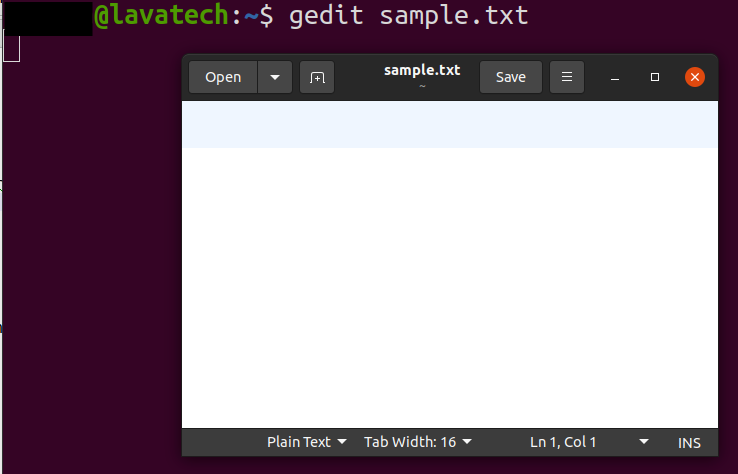
\includegraphics[scale=0.4]{content/chapter3/images/gedit.png}
				\caption{Sample output}
				\label{fig:cal32}
			\end{figure}
			
		\end{itemize}
		\item \textbf{Text-based editor}
		\begin{itemize}
			\item \textbf{vi or vim}:  Text based editor used in Linux and Mac OS. Let's see more on this.
		\end{itemize}
	\end{itemize}
\end{flushleft}

\newpage






\subsection{Vi/vim in detail}
\setlength{\columnsep}{3pt}
\begin{flushleft}
	\bigskip
	\paragraph{What is vi editor?}
	\begin{itemize}
		\item Vi is a free and open source, screen-based text editor program for Linux/Unix OS.
	\end{itemize}
	\paragraph{What is vim editor?}
	\begin{itemize}
		\item Vim is an advance version of vi.
		
	We are going to explore "vim" editor in detail as it is more advance than "vi".

	\paragraph{How to use vi or vim editor?}
			\bigskip
			\begin{tcolorbox}[breakable,notitle,boxrule=1pt,colback=black,colframe=black]
				\color{green}
				\fontdimen2\font=1em
				\# vim one.txt
				\newline
				or
				\newline
				\# vi one.txt
				\fontdimen2\font=4pt
			\end{tcolorbox}
			This will open an editor in front of you as shown:
			\begin{figure}[h!]
			\centering
			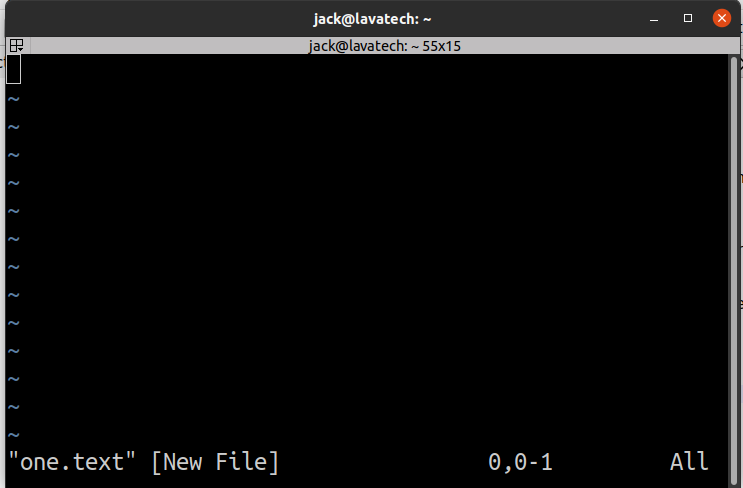
\includegraphics[scale=.4]{content/chapter3/images/vim.png}
			\caption{Vim Editor}
			\label{fig:vim_editor}
		\end{figure}
\end{flushleft}

\newpage






\subsection{Moving around file using vi/vim}

\begin{flushleft}
	
	There are two modes using which you can navigate \& edit a file in vim:
	\begin{itemize}

		\item \textbf{Command mode}: 
		\begin{itemize}
			\item \textbf{Press Esc} to enter command mode.
			\item This is default mode.
			\item File cannot be edited under this mode.
			\item Below keystrokes will move the cursor:
			\begin{itemize}	
				\item \textbf{\$}: Move cursor to the end of the line.
				\item \textbf{17G}: Move cursor to line 17 (i.e type 17 and press shift + g).
				\item \textbf{G}: Move cursor to the last line (i.e press shift + g).
			\end{itemize}
			
		\end{itemize}

		\newline
		\bigskip
		
		\bigskip
		\bigskip
		\item \textbf{Insert mode}: 
		\begin{itemize}
			\item \textbf{Press i or a or o} to enter insert mode.
			\item This mode is used to edit the file.
			\item Below keystrokes will allow you to enter this mode:
			\begin{itemize}
				\item \textbf{i}: Insert text just \textbf{before} the current cursor position.
				\item \textbf{a}: Insert text just \textbf{after} the current cursor position.
				\item \textbf{o}: Insert text into a \textbf{new line} below current line.
				\item \textbf{I}: Insert text at the \textbf{beginning} of the current line.
				\item \textbf{A}: Insert text at the \textbf{end} of the current line.
				\item \textbf{O}: Insert text into a \textbf{new line} above current line.
			\end{itemize}
			
		\end{itemize}

					
	
		
		

	\end{itemize}
	
	
\end{flushleft}

\newpage

\subsection{Searching for text using vi/vim}

\begin{flushleft}

You can search a specific word in vim editor:
\newline
\textbf{Forward search:}
\begin{itemize}
	\item \textbf{Press ESC} to switch to command mode.
	\item \textbf{Press "/"} and type the word to search.
	\newline
	Eg: \textbf{/bunny and press enter}: Jump forward to the first occurrence of the string "bunny" after current cursor position.
	\item \textbf{press n}: Jumps to the next occurrence of the word searched by "/".
	\item \textbf{press N}: Jumps to the previous occurrence of the word searched by “/”.
\end{itemize}

\bigskip\bigskip
\textbf{Backward search:}
\begin{itemize}
	\item \textbf{Press ESC} to switch to command mode.
	\item \textbf{Press "?"} and type the word to search.
	\newline
	Eg: \textbf{?bunny and press enter}: Jump backward to the first occurrence of the string "bunny" before current cursor position.
	\item \textbf{press n}: Jumps to the next occurrence of the word searched by "?".
	\item \textbf{press N}: Jumps to the previous occurrence of the word searched by “?”.
\end{itemize}


\end{flushleft}
\newpage
\subsection{Saving and/or quitting the file using vi/vim}

\begin{flushleft}
	
	
	\bigskip
	File can by saved and/or quitted in vim editor. 
	\newline
	To do this, \textbf{switch to command mode (by pressing Esc)} and then do any of the following:
	\begin{itemize}
		\item \textbf{:wq} or \textbf{:x} and press enter-  \textbf{Save \& quit} the edited file.
		\item \textbf{:q!} and press enter - \textbf{Quit} the editor without saving changes.
		\item \textbf{:w} and press enter - \textbf{Save} the edited file without quitting.
	\end{itemize}
		
\end{flushleft}
\newpage
\subsection{More functions in vi/vim}

\begin{flushleft}
	
	
	\bigskip
	Other useful functions in command mode (\textbf{press Esc to switch to command mode}) are:
	\begin{itemize}
		\item \textbf{u} - Undo the last change to the file (and type "u" again to re-do the change).
		\item \textbf{U} - Undo all changes to the current line.
		\item \textbf{yy} - Copy a line.
		\item \textbf{p} - Paste a line.
		\item \textbf{dd} - Delete a line.
		\item \textbf{yy} - Copy a single line.
		\item \textbf{Nyy} - Copy N number of lines. Eg: To copy 5 lines, press 5yy.
		\item \textbf{p} - Paste a single line.
		\item \textbf{Np} - Paste N number of times a copied line. Eg: To paste a line 5 times, press 5p.
		\item \textbf{dd} - Delete a single line.
		\item \textbf{Ndd} - Delete N number of lines. Eg: To delete 5 lines, press 5dd.
		\item \textbf{:set nu and press enter} - Show all line numbers .
		\item \textbf{:set nonu and press enter} - Removes all line numbers.
		\item \textbf{:s/Joe/Bob and press enter} - Substitute first occurrence of Joe in current line by Bob.
		\item \textbf{:s/Joe/Bob/g and press enter} - Substitute all occurrences of Joe in current line by Bob.
		\item \textbf{:\%s/Joe/Bob/g and press enter} - Substitute every "Joe" to "Bob" throughout the
		document.
	\end{itemize}
	
\end{flushleft}
\newpage
\subsection{Practice}
\setlength{\columnsep}{3pt}
\begin{flushleft}
	\paragraph{}
	
	\bigskip
	
	\begin{figure}[h!]
		\centering
		\includegraphics[scale=.2]{content/practise.jpg}
	\end{figure}	
	
	\begin{enumerate}
		\item \textbf{Which of the following combination is used to save and exit a file in vim editor? (Select all that applies.)}
		\begin{enumerate}[label=(\alph*)]
			\item :x       %correct
			\item :wq      %correct
			\item :wq!                  % correct
			\item :w
		\end{enumerate}
		\bigskip
		\bigskip
		\item \textbf{Which of the following keystroke is used to undo changes in vim editor? (Select all that applies.)}
		\begin{enumerate}[label=(\alph*)]
			\item Press "z" in command mode      
			\item Press "U" in command mode    %correct
			\item Press "u" in command mode   %correct
			\item Press "s" in command mode
		\end{enumerate}
		\bigskip
		\bigskip
		\item \textbf{Which of the following keystroke is used to enter in \textbf{inset mode} in vim editor? (Select all that applies.)}
		\begin{enumerate}[label=(\alph*)]
			\item Press "a" %correct
			\item Press "i" %correct
			\item Press "o" %correct
			\item Press "z"
		\end{enumerate}
		\bigskip
		\bigskip
		\item \textbf{Which of the following keystroke is used to enter in \textbf{command mode} in vim editor?}
		\begin{enumerate}[label=(\alph*)]
			\item Press "CTRL"
			\item Press "ATL"
			\item Press "SHIFT"
			\item Press "ESC"  %correct
		\end{enumerate}
		\bigskip
		\bigskip
		\item \textbf{Which of the following keystroke is used to delete a line in vim editor?}
		\begin{enumerate}[label=(\alph*)]
			\item Press "d" in command mode      
			\item Press "y" in command mode      
			\item Press "p" in command mode      
			\item Press "dd" in command mode        %correct
		\end{enumerate}
		\bigskip
		\bigskip
		\item \textbf{Which of the following keystroke is used to copy 5 lines in vim editor?}
		\begin{enumerate}[label=(\alph*)]
			\item Press "5y" in command mode      
			\item Press "5yy" in command mode        %correct
			\item Press "5p" in command mode      
			\item Press "5dd" in command mode     
		\end{enumerate}	
		\bigskip
		\bigskip
		\item \textbf{Which of the following keystroke is used to paste a line 10 times in vim editor?}
		\begin{enumerate}[label=(\alph*)]
			\item Press "10p" in command mode      
			\item Press "10pp" in command mode        %correct
			\item Press "10y" in command mode      
			\item Press "10yy" in command mode     
		\end{enumerate}	
		\bigskip
		\bigskip
		\item \textbf{Which of the following string helps in setting line numbers in vim editor?}
		\begin{enumerate}[label=(\alph*)]
			\item \textbf{:set nu} in command mode   %correct
			\item \textbf{:set line} in command mode   
			\item \textbf{:s/nu} in command mode  
			\item \textbf{:set nonu} in command mode  
		\end{enumerate}
		\bigskip
		\bigskip
		\item \textbf{Which of the following string is used substitute a word in entire file in vim editor?}
		\begin{enumerate}[label=(\alph*)]
			\item \textbf{:replace/old\_word/new\_word/} in command mode   
			\item \textbf{:s/old\_word/new\_word/g} in command mode 
			\item \textbf{:\%s/old\_word/new\_word/g} in command mode    %correct
			\item \textbf{:set nu} in command mode  
		\end{enumerate}
	\end{enumerate}
	
	
\end{flushleft}
\newpage

\afterpage{\blankpage}

%-----------------------

%----------------------------------------------------------------------------------------
%	CHAPTER 4
%----------------------------------------------------------------------------------------
\chapterimage{index5.png} % Table of contents heading image
\chapter{User \& Group Administration}
%-----------------------
\section{User \& group basics}\index{User \& group basics}
\setlength{\columnsep}{3pt}
\begin{flushleft}
	\bigskip
	\bigskip
	\begin{tcolorbox}[breakable,notitle,boxrule=1pt,colback=black,colframe=black]
		\color{white}
		\bigskip
		In this section, you are going to learn:
		\begin{enumerate}
			\item \textbf{What is a user \& group?}
			\item \textbf{Types of group}
			\item \textbf{Files containing user \& group details}
		\end{enumerate}	
		\bigskip
		Finally, there will be a \textbf{small excerise} on these topics to check your knowledge.
		\bigskip
	\end{tcolorbox}
	
	
	\begin{multicols}{2}
		\vspace*{\fill}
		\vspace*{\fill}
		\vspace*{\fill}
		\vspace*{\fill}
		\vspace*{\fill}
		\vspace*{\fill}
		\vspace*{\fill}
		\vspace*{\fill}
		\vspace*{\fill}
		
		\vfill \null
		\columnbreak
		So let's get started....
		\includegraphics[scale=0.08]{content/linux_section.png}
	\end{multicols}	
	
\end{flushleft}

\newpage


\subsection{What is a user?}\index{User \& group basics!What is a user?}
\setlength{\columnsep}{3pt}
\begin{flushleft}
	\bigskip
	To login to any UNIX machine, you need a user. There are 3 types of users in Linux:

	\begin{figure}[h!]
		\centering
		\includegraphics[scale=0.20]{content/chapter4/images/users.png}
		\caption{User types}
		\label{fig:user}
	\end{figure}

	
	\begin{itemize}
		\item \textbf{Superuser i.e. root}: 
		\begin{itemize}
			\item Automatically created when you install Linux.
			\item Superuser can execute commands under \textbf{/usr/sbin \& /usr/bin}.
		\end{itemize}

		\item \textbf{System users}:
		\begin{itemize}
			\item Created automatically during application or software installation.
			\item Eg: When you install VLC media player in Linux, a user named "vlc" will be created automatically.
			\item These accounts exist to allow different services to interact with
			your computer.
		\end{itemize}
		
		\item \textbf{Normal or Local users}:
		\begin{itemize}
			\item Created by root or sudo user.
			\item Local user can execute commands under \textbf{/usr/bin}.
			\item Eg: jack, jill, ram, ravi etc.
		\end{itemize}
		
	\end{itemize}

\end{flushleft}

\newpage






\subsection{What is a group?}\index{User \& group basics!What is a group?}
\setlength{\columnsep}{3pt}
\begin{flushleft}
	\bigskip
	\begin{figure}[h!]
	\centering
	\includegraphics[scale=.2]{content/chapter4/images/user_group.jpg}
	\caption{User V/S Group}
	\label{fig:user_group}
	\end{figure}
	\bigskip

	\begin{itemize}
		\item Group is a collection of users.
		\item Users are grouped together for granting common permissions to all members of a group.
		\item A user can be a member of more than one group.
	\end{itemize}

\newpage
	\paragraph{Types of group}
	
	\begin{itemize}
		\item \textbf{Primary group}:
		\begin{itemize}
			\item Primary group are automatically generated while creating a user.
			\item A user becomes member of their primary group automatically.
			\item Primary group have same name as the username \& a unique group ID.
			\item \textbf{One user can have one and only one primary group}.
		\end{itemize} 
		\item \textbf{Secondary or supplementary group}:
		\begin{itemize}
			\item Secondary group are created separately with the help of \textbf{groupadd} command.
			\item Multiple users can be added to the secondary group.
			\item \textbf{One user can have more than one secondary groups}.
		\end{itemize} 
	\end{itemize}
	
	\begin{figure}[h!]
		\centering
		\includegraphics[scale=0.5]{content/chapter4/images/type_group.png}
		\caption{Primary and Secondary group}
		\label{fig:prime_secondary_group}
	\end{figure}
	


\end{flushleft}

\newpage


\subsection{Files containing user \& group details}
\setlength{\columnsep}{3pt}
\begin{flushleft}

	Below diagram shows important files and their short description relating to user \& group details:
	\begin{figure}[h!]
	\centering
	\includegraphics[scale=0.4]{content/chapter4/images/users6.png}
	\caption{Important user \& group files}
	\label{fig:prime_secondary_group12}
\end{figure}

Let's see each of these file in detail.

\newpage

\textbf{Structure of /etc/passwd file}
\begin{itemize}
	\item Fields in this file are separated by a ":" (colon).
	\begin{figure}[h!]
	\centering
	\includegraphics[scale=.2]{content/chapter4/images/53.png}
	\caption{Sample /etc/passwd entry}
	\label{fig:user_group1}
	\end{figure}	
	\newline
Explaination:
\begin{enumerate}
	\item \textbf{Username} - Case-sensitive login name of user.
	\item \textbf{Password placeholder} - "x" acts as placeholder. Encrypted password are now stored in \textbf{/etc/shadow} file.
	\item \textbf{User ID}: UID ranges:
		\begin{itemize}
		\item UID 0 is assigned to root user.
		\item UID 1-200 is a range of "system users" assigned to system processes by OS.
		\item UID 201-999 is a range of "system users" used by system processes.
		\item UID 1000+ is the range available for assignment to regular users.
	\end{itemize}
	\item \textbf{Group ID}
	\item \textbf{Comment} - More description about user.
	\item \textbf{Home directory} - Location of user's personal data.
	\item \textbf{Shell} - User login shell, default is \textbf{/bin/bash}.
\end{enumerate}

\end{itemize}	
\newpage



\textbf{Structure of the /etc/shadow file}
\begin{itemize}
	\item Fields in this file are separated by a ":" (colon).
	\begin{figure}[h!]
		\centering
		\includegraphics[scale=.4]{content/chapter4/images/pass4.png}
		\caption{Sample /etc/shadow entry}
		\label{fig:user_group}
	\end{figure}	
	\newline
	Explaination:
	\begin{enumerate}
		\item \textbf{Username} - A direct match to the username in the \textbf{/etc/passwd} file.
		\item \textbf{Encrypted Password} - Store password in encrypted format.
		\bigskip
		\begin{tcolorbox}[breakable,notitle,boxrule=-0pt,colback=yellow,colframe=yellow]
			\color{black}
			\textbf{Note:} 
			\begin{itemize}
				\item \textbf{“!”} in this entry means the account is disabled or locked. 
				\item \textbf{“!!”} mask means password is not assigned.
			\end{itemize}
		\end{tcolorbox}	
		Let's understand the encrypted password in detail.
		\newpage	
		\begin{figure}[h!]
			\centering
			\includegraphics[scale=.5]{content/chapter4/images/pass.png}
		\end{figure}
		There are three pieces of information stored in password:
		\begin{itemize}
			\item \textbf{Hashing algorithm}: The number 1 indicates an MD5 hash. The number 6 appears when a SHA-512 hash is used.
			\item \textbf{Salt value}: The random salt value used to encrypt the hash. Prevents two users with the same password from having identical entries in the /etc/shadow file.
			\item \textbf{Encrypted hash}
		\end{itemize}
		\bigskip
		\bigskip
		\item \textbf{Password age}:
		\begin{figure}[h!]
			\centering
			\includegraphics[scale=.2]{content/chapter4/images/age.png}
		\end{figure}
		\begin{enumerate}\addtocounter{enumi}{3}
			\item \textbf{Last password change} - The number of days (since January 1, 1970) since the password was last changed.
			\item \textbf{Minimum days before password change} - The number of days before password may be changed (0 indicates it may be changed at any time).
			\item \textbf{Maximum days before password change} - The number of days after which password must be changed (99999 indicates user can keep his or her password unchanged for many, many years).
			\item \textbf{Password change warning} - The number of days to warn user of an expiring password (7 for a full week).
			\item \textbf{Account active days} - The number of days an account remains active after a password has expired.
			\item \textbf{No. of days account is expired} - The account expiration date, represented as the number of days since 1970.01.01.
			\item This blank field is reserved for future use.
		\end{enumerate}
	\end{enumerate}
\end{itemize}	
	
\newpage

\textbf{Structure of the /etc/group file}
\begin{itemize}
	\item Fields in this file are separated by a ":" (colon).
	\begin{figure}[h!]
		\centering
		\includegraphics[scale=.2]{content/chapter4/images/54.png}
		\caption{Sample /etc/group entry}
		\label{fig:user_group}
	\end{figure}	
	\newline
	Explaination
	\begin{itemize}
		\item Column 1: \textbf{Groupname} - Name of group. It is case-sensitive. 
		\item Column 2: \textbf{Group password placeholder} - "x" acts as placeholder. Encrypted password are stored in \textbf{/etc/gshadow} file.
		\item Column 3: \textbf{Group ID} 
		\item Column 4: \textbf{Group members} - Usernames of users belonging to this group.
	\end{itemize}	
\end{itemize}	

\newpage
\textbf{Structure of the /etc/gshadow file}
\begin{itemize}
	\item Fields in this file are separated by a ":" (colon).
	\begin{figure}[h!]
		\centering
		\includegraphics[scale=.2]{content/chapter4/images/56.png}
		\caption{Sample /etc/gshadow entry}
		\label{fig:user_group}
	\end{figure}	
	\newline
	Explaination:
	\begin{itemize}
		\item Column 1: \textbf{Groupname} - Name of group. It is case-sensitive. 
		\item Column 2: \textbf{Encrypted Password} - Store password in encrypted format.
		\bigskip
		\begin{tcolorbox}[breakable,notitle,boxrule=-0pt,colback=yellow,colframe=yellow]
			\color{black}
			\textbf{Note:} 
			\begin{itemize}
				\item {“!”} in this entry means the account is disabled or locked. 
				\item {“!!”} mask means password is not assigned.
			\end{itemize}
		\end{tcolorbox}

		\item Column 3: \textbf{Administrators} - Users who can change the password.
		\item Column 4: \textbf{Group members} - Usernames of user belonging to this group.
	\end{itemize}	
\end{itemize}	

	
\end{flushleft}

\newpage


\subsection{Practice}\index{User \& group basics!Practice}
\setlength{\columnsep}{3pt}
\begin{flushleft}
	\paragraph{}
	
	\bigskip
	
	\begin{figure}[h!]
		\centering
		\includegraphics[scale=.2]{content/practise.jpg}
	\end{figure}	
	
	\begin{enumerate}
		\item \textbf{State whether true or false. One user can have one \& only one primary group and 0 or more secondary groups.}
		\begin{enumerate}[label=(\alph*)]
			\item True %correct
			\item False
		\end{enumerate}
		\bigskip
		\bigskip
		\item \textbf{Which of the following file contains user details?}
		\begin{enumerate}[label=(\alph*)]
			\item /etc/shadow
			\item /etc/skel
			\item /etc/group
			\item /etc/passwd %correct
		\end{enumerate}
		\bigskip
		\bigskip
		\item \textbf{Which of the following file contains user password details?}
		\begin{enumerate}[label=(\alph*)]
			\item /etc/group
			\item /etc/gshadow
			\item /etc/shadow  %correct
			\item /etc/passwd
		\end{enumerate}
		\bigskip
		\bigskip
		\item \textbf{State whether true or false. Default shell of user is /bin/bash.}
		\begin{enumerate}[label=(\alph*)]
			\item True  %correct
			\item False
		\end{enumerate}
		\bigskip
		\bigskip
		\item \textbf{State whether true or false. Group is collection of users.}
		\begin{enumerate}[label=(\alph*)]
			\item True  %correct
			\item False
		\end{enumerate}
		\bigskip
		\bigskip
		\item \textbf{Which of the following are valid fields of /etc/passwd file? (Select all that applies.)}
		\begin{enumerate}[label=(\alph*)]
			\item shell                  %correct
			\item home directory        %correct
			\item comment	%correct
			\item username	%correct
		\end{enumerate}
		\bigskip
		\bigskip
		\item \textbf{State whether true or false. Primary group is created automatically at the time of user creation.}
		\begin{enumerate}[label=(\alph*)]
			\item True       %correct
			\item False
		\end{enumerate}
		\bigskip
		\bigskip
		\item \textbf{State whether true or false. Secondary group is created automatically at the time of user creation.}
		\begin{enumerate}[label=(\alph*)]
			\item True       
			\item False  %correct
		\end{enumerate}
	\end{enumerate}
	
	
\end{flushleft}
\newpage




\section{User \& group commands}\index{User \& group commands}
\setlength{\columnsep}{3pt}
\begin{flushleft}
	\bigskip
	\bigskip
	\begin{tcolorbox}[breakable,notitle,boxrule=1pt,colback=black,colframe=black]
		\color{white}
		\bigskip
		In this section, you are going to learn:
		\begin{enumerate}
			\item \textbf{User commands}
			\item \textbf{Content of /etc/skel directory}
			\item \textbf{Group commands}
		\end{enumerate}	
		\bigskip
		Finally, there will be a \textbf{small excerise} on these topics to check your knowledge.
		\bigskip
	\end{tcolorbox}
	
	
	\begin{multicols}{2}
		\vspace*{\fill}
		\vspace*{\fill}
		\vspace*{\fill}
		\vspace*{\fill}
		\vspace*{\fill}
		\vspace*{\fill}
		\vspace*{\fill}
		\vspace*{\fill}
		\vspace*{\fill}
		
		\vfill \null
		\columnbreak
		So let's get started....
		\includegraphics[scale=0.08]{content/linux_section.png}
	\end{multicols}	
	
\end{flushleft}

\newpage


\subsection{User commands}\index{User \& group commands!User commands}
\setlength{\columnsep}{3pt}
\begin{flushleft}
	
	Let's see some commands to create, update \& delete users in Linux OS.
	
	\paragraph{How to create a new user?}
	\bigskip
	\textbf{useradd}: Create a new user.
	\begin{tcolorbox}[breakable,notitle,boxrule=1pt,colback=pink,colframe=pink]
		\color{black}
		\fontdimen2\font=1em
		Syntax:  useradd username
		\fontdimen2\font=4pt
	\end{tcolorbox}
	On adding a new user, a user have below things set:
	\begin{itemize}
		\item Home directory: \textbf{/home/username}
		\item Default shell: \textbf{/bin/bash}
		\item Primary group: Named same as \textbf{username}
		\item Password: \textbf{No password is set}
	\end{itemize}
	
	\begin{tcolorbox}[breakable,notitle,boxrule=1pt,colback=yellow,colframe=yellow]
		\color{black}
		Note: Some defaults, such as the UID numbers and default password aging rules, are read from the \textbf{/etc/login.defs} file.
	\end{tcolorbox}
	
	Options with \textbf{useradd} command:
	\begin{enumerate}[label=(\alph*)]
		\item \textbf{–g}: Assign primary group.
		\bigskip
		\begin{tcolorbox}[breakable,notitle,boxrule=0pt,colback=pink,colframe=pink]
			\color{black}
			\fontdimen2\font=1em
			Syntax: useradd -g primary\_group\_name username
			\fontdimen2\font=4pt
		\end{tcolorbox}
		Eg:
		\bigskip
		\begin{tcolorbox}[breakable,notitle,boxrule=-0pt,colback=black,colframe=black]
			\color{green}
			\fontdimen2\font=1em
			\# useradd –g javadevl shekhar
			\fontdimen2\font=4pt
		\end{tcolorbox}
		
		\item \textbf{–G}: Assign secondary groups.
		\bigskip
		\begin{tcolorbox}[breakable,notitle,boxrule=0pt,colback=pink,colframe=pink]
			\color{black}
			\fontdimen2\font=1em
			Syntax: useradd -G secondary\_group\_name username
			\fontdimen2\font=4pt
		\end{tcolorbox}
		Eg:
		\bigskip
		\begin{tcolorbox}[breakable,notitle,boxrule=-0pt,colback=black,colframe=black]
			\color{green}
			\fontdimen2\font=1em
			\# useradd –G cdevl,perldevl shekhar
			\fontdimen2\font=4pt
		\end{tcolorbox}
		
		\newpage
		\item \textbf{–u}: Assign specific UID. UID should be more than 500 for normal users.
		\bigskip
		\begin{tcolorbox}[breakable,notitle,boxrule=0pt,colback=pink,colframe=pink]
			\color{black}
			\fontdimen2\font=1em
			Syntax: useradd –u UID username
			\fontdimen2\font=4pt
		\end{tcolorbox}
		Eg:
		\bigskip
		\begin{tcolorbox}[breakable,notitle,boxrule=-0pt,colback=black,colframe=black]
			\color{green}
			\fontdimen2\font=1em
			\# useradd –u 601 shekhar
			\fontdimen2\font=4pt
		\end{tcolorbox}
		
		
		\item \textbf{–s}: Change user shell.
		\bigskip
		\begin{tcolorbox}[breakable,notitle,boxrule=0pt,colback=pink,colframe=pink]
			\color{black}
			\fontdimen2\font=1em
			Syntax: useradd –s shell\_name username
			\fontdimen2\font=4pt
		\end{tcolorbox}
		Eg:
		\bigskip
		\begin{tcolorbox}[breakable,notitle,boxrule=-0pt,colback=black,colframe=black]
			\color{green}
			\fontdimen2\font=1em
			\# useradd –s /sbin/nologin shekhar
			\fontdimen2\font=4pt
		\end{tcolorbox}
		\bigskip
		\begin{tcolorbox}[breakable,notitle,boxrule=-0pt,colback=yellow,colframe=yellow]
			\color{black}
			Note: Shell \textbf{/sbin/nologin} will not allow username to login. Usually used for system users like ftp, squid etc.
		\end{tcolorbox}
		
		
		\item \textbf{–d}: Change user's home directory.
		\bigskip
		\begin{tcolorbox}[breakable,notitle,boxrule=0pt,colback=pink,colframe=pink]
			\color{black}
			\fontdimen2\font=1em
			Syntax: useradd –d directory\_name username
			\fontdimen2\font=4pt
		\end{tcolorbox}
		Eg:
		\bigskip
		\begin{tcolorbox}[breakable,notitle,boxrule=-0pt,colback=black,colframe=black]
			\color{green}
			\fontdimen2\font=1em
			\# useradd –d /mnt/shekar shekhar 
			\fontdimen2\font=4pt
		\end{tcolorbox}
	\end{enumerate}
	
	\bigskip
	\bigskip
	
	\newpage
	
	\paragraph{How to assign or change user’s password?}
	
	\bigskip
	\textbf{passwd}: Assign/change user's password.
	
	\begin{tcolorbox}[breakable,notitle,boxrule=0pt,colback=pink,colframe=pink]
		\color{black}
		\fontdimen2\font=1em
		Syntax: passwd username
		\fontdimen2\font=4pt
	\end{tcolorbox}
	On executing the command, you will be asked to set password twice.
	
	\begin{tcolorbox}[breakable,notitle,boxrule=0pt,colback=yellow,colframe=yellow]
		\color{black}
		Note: 
		\begin{itemize}
			\item Root user or superuser can set the password of any user.
			\item Local user can set their own password, but not of anyone else.
		\end{itemize}

	\end{tcolorbox}
	
	Options with \textbf{passwd} command:
	
	\begin{itemize}
		\item \textbf{- -stdin}: Change password by providing it on command line itself.
		\begin{tcolorbox}[breakable,notitle,boxrule=0pt,colback=pink,colframe=pink]
			\color{black}
			\fontdimen2\font=1em
			Syntax: echo “new\_password” | passwd ---stdin username
			\fontdimen2\font=4pt
		\end{tcolorbox}
		Eg:
		\bigskip
		\begin{tcolorbox}[breakable,notitle,boxrule=-0pt,colback=black,colframe=black]
			\color{green}
			\fontdimen2\font=1em
			\# echo “shekhar@12345” | passwd ---stdin shekhar
			\fontdimen2\font=4pt
		\end{tcolorbox}
	\end{itemize}
\newpage

\newpage
\paragraph{How to change user’s password attributes?}

\bigskip
\textbf{chage}: Changing the password aging information for user.

\begin{tcolorbox}[breakable,notitle,boxrule=0pt,colback=pink,colframe=pink]
	\color{black}
	\fontdimen2\font=1em
	Syntax: chage username
	\fontdimen2\font=4pt
\end{tcolorbox}
Eg:
\begin{figure}[h!]
	\centering
	\includegraphics[scale=.5]{content/chapter4/images/chage1.png}
	\caption{Sample output}
	\label{fig:command_prompt5}
\end{figure}

Options with \textbf{chage} command:

\begin{itemize}
	\item \textbf{-l}: Show account aging information.
	\begin{tcolorbox}[breakable,notitle,boxrule=0pt,colback=pink,colframe=pink]
		\color{black}
		\fontdimen2\font=1em
		Syntax: chage -l username
		\fontdimen2\font=4pt
	\end{tcolorbox}
	Eg:
	\bigskip
	\begin{figure}[h!]
		\centering
		\includegraphics[scale=.5]{content/chapter4/images/chage2.png}
		\caption{Sample output}
		\label{fig:command_prompt8}
	\end{figure}
\end{itemize}

\newpage

\paragraph{Switch between users}
\begin{itemize}
	\item \textbf{su}: Allows a user to switch to a different user account. If a username is not specified, the root account is implied.
		\begin{tcolorbox}[breakable,notitle,boxrule=0pt,colback=pink,colframe=pink]
		\color{black}
		\fontdimen2\font=1em
		Syntax: su [-] [username]
		\fontdimen2\font=4pt
	\end{tcolorbox}
	Eg:
	\bigskip
	\begin{tcolorbox}[breakable,notitle,boxrule=-0pt,colback=black,colframe=black]
		\color{green}
		\fontdimen2\font=1em
		\# su - jack
		\fontdimen2\font=4pt
	\end{tcolorbox}
	What is used of "-" in su command?
	\begin{itemize}
		\item The command \textbf{"su username"} starts a non-login shell, while the command \textbf{"su - username"} starts a login shell. 
		\item The main distinction is \textbf{"su -"} sets up the shell environment as if this were a clean login as that user, while \textbf{"su"} just starts a shell as that user with the current environment settings.
	\end{itemize}
\end{itemize}

\paragraph{Running command as root with sudo}
\begin{itemize}
	\item \textbf{sudo}: Allows a user to be permitted to run a command as root, or as another user,
	based on settings in the /etc/sudoers file.
	\begin{tcolorbox}[breakable,notitle,boxrule=0pt,colback=pink,colframe=pink]
		\color{black}
		\fontdimen2\font=1em
		Syntax: sudo command
		\fontdimen2\font=4pt
	\end{tcolorbox}
	Eg:
	\bigskip
	\begin{tcolorbox}[breakable,notitle,boxrule=-0pt,colback=black,colframe=black]
		\color{green}
		\fontdimen2\font=1em
		\$ sudo useradd raman
		\fontdimen2\font=4pt
	\end{tcolorbox}
\end{itemize}

	
	\newpage
	
	\paragraph{How to modify an existing user?}
	\bigskip
	\textbf{usermod}: Modify existing user.
	\newline
	Options with \textbf{usermod} command:
	\begin{enumerate}[label=(\alph*)]
		\item \textbf{–g}: Change user's primary group.
		\bigskip
		\begin{tcolorbox}[breakable,notitle,boxrule=0pt,colback=pink,colframe=pink]
			\color{black}
			\fontdimen2\font=1em
			Syntax: usermod –g primary\_group username
			\fontdimen2\font=4pt
		\end{tcolorbox}
		Eg:
		\bigskip
		\begin{tcolorbox}[breakable,notitle,boxrule=-0pt,colback=black,colframe=black]
			\color{green}
			\fontdimen2\font=1em
			\# usermod –g cdevl shekhar
			\fontdimen2\font=4pt
		\end{tcolorbox}
		
		\item \textbf{–G}: Change user's secondary group.
		\bigskip
		\begin{tcolorbox}[breakable,notitle,boxrule=0pt,colback=pink,colframe=pink]
			\color{black}
			\fontdimen2\font=1em
			Syntax: usermod -G secondary\_group\_name username
			\fontdimen2\font=4pt
		\end{tcolorbox}
		Eg:
		\bigskip
		\begin{tcolorbox}[breakable,notitle,boxrule=-0pt,colback=black,colframe=black]
			\color{green}
			\fontdimen2\font=1em
			\# usermod –G javadevl shekhar
			\fontdimen2\font=4pt
		\end{tcolorbox}
		
		
		\item \textbf{–L}: Lock (i.e. disable) user.
		\bigskip
		\begin{tcolorbox}[breakable,notitle,boxrule=0pt,colback=pink,colframe=pink]
			\color{black}
			\fontdimen2\font=1em
			Syntax: usermod -L username
			\fontdimen2\font=4pt
		\end{tcolorbox}		
		
		\item \textbf{–U}: Unlock user account.
		\bigskip
		\begin{tcolorbox}[breakable,notitle,boxrule=0pt,colback=pink,colframe=pink]
			\color{black}
			\fontdimen2\font=1em
			Syntax: usermod –U username
			\fontdimen2\font=4pt
		\end{tcolorbox}
		
		\item \textbf{–s}: Change user's login shell.
		\bigskip
		\begin{tcolorbox}[breakable,notitle,boxrule=0pt,colback=pink,colframe=pink]
			\color{black}
			\fontdimen2\font=1em
			Syntax: usermod –s shell\_name username
			\fontdimen2\font=4pt
		\end{tcolorbox}
		Eg:
		\bigskip
		\begin{tcolorbox}[breakable,notitle,boxrule=-0pt,colback=black,colframe=black]
			\color{green}
			\fontdimen2\font=1em
			\# usermod –s /bin/ksh shekhar
			\fontdimen2\font=4pt
		\end{tcolorbox}
		
		\newpage
		\item \textbf{–d}: Change user's home directory.
		\item \textbf{-m}: Create user's new home directory.
		\bigskip
		\begin{tcolorbox}[breakable,notitle,boxrule=0pt,colback=pink,colframe=pink]
			\color{black}
			\fontdimen2\font=1em
			Syntax: usermod –d directory\_name username -m
			\fontdimen2\font=4pt
		\end{tcolorbox}
		Eg:
		\bigskip
		\begin{tcolorbox}[breakable,notitle,boxrule=-0pt,colback=black,colframe=black]
			\color{green}
			\fontdimen2\font=1em
			\# usermod –d /opt/java shekhar -m
			\fontdimen2\font=4pt
		\end{tcolorbox}
	\end{enumerate}
	
	\bigskip
	\bigskip
	
	\newpage
	
	\paragraph{How to delete a user?}
	
	\bigskip
	\begin{tcolorbox}[breakable,notitle,boxrule=-0pt,colback=red,colframe=red]
		\color{white}
		Standard Practice: You should not delete a user if they leave	 the organization. You
		should lock their account.
	\end{tcolorbox}
	
	
	
	\textbf{userdel}: Delete user \& remove it's entry from \textbf{/etc/passwd} and \textbf{/etc/shadow} files.
	\begin{tcolorbox}[breakable,notitle,boxrule=0pt,colback=pink,colframe=pink]
		\color{black}
		\fontdimen2\font=1em
		Syntax: userdel username
		\fontdimen2\font=4pt
	\end{tcolorbox}
	Eg:
	\begin{tcolorbox}[breakable,notitle,boxrule=-0pt,colback=black,colframe=black]
		\color{green}
		\fontdimen2\font=1em
		\# userdel shekhar
		\fontdimen2\font=4pt
	\end{tcolorbox}

	\begin{tcolorbox}[breakable,notitle,boxrule=-0pt,colback=yellow,colframe=yellow]
		\color{black}
		Note: userdel command does not delete user's home directory by default.
	\end{tcolorbox}	

	Options with \textbf{userdel} command:
	\begin{itemize}
		\item \textbf{-r}: Delete user along with home directory.
		\begin{tcolorbox}[breakable,notitle,boxrule=0pt,colback=pink,colframe=pink]
			\color{black}
			\fontdimen2\font=1em
			Syntax: userdel -r username
			\fontdimen2\font=4pt
		\end{tcolorbox}
		Eg:
		\begin{tcolorbox}[breakable,notitle,boxrule=-0pt,colback=black,colframe=black]
			\color{green}
			\fontdimen2\font=1em
			\# userdel -r shekhar
			\fontdimen2\font=4pt
		\end{tcolorbox}
	\end{itemize}
	
\end{flushleft}

\newpage


\subsection{Content of /etc/skel directory}\index{User \& group commands!Content of /etc/skel directory}
\setlength{\columnsep}{3pt}
\begin{flushleft}

\textbf{/etc/skel} directory:
\begin{itemize}
	\item Content of this directory is \textbf{automatically copied over to a new user's home directory when it is created}.
	\item Users gets same intial settings and environment using content of this directory.
	\item Below are the files under \textbf{/etc/skel} directory that are copied:
	\begin{itemize}
		\item \textbf{/etc/skel/.bash\_profile} copied as \textbf{{$\sim$}/.bash\_profile}: 
		\begin{itemize}
			\item Configures the bash startup environment.
			\item You can the add environment variables to this file.
		\end{itemize}
		\bigskip
		\item \textbf{/etc/skel/.bashrc} copied as \textbf{{$\sim$}/.bashrc}: 
		\begin{itemize}
			\item In this file you can include commands you want to run when you start the bash shell.
			\item You can also add aliases such as: \textbf{rm='rm -i'}
		\end{itemize}
		\bigskip
		\item \textbf{/etc/skel/.bash\_logout} copied as \textbf{{$\sim$}/.bash\_logout}: 
		\newline
		This file is executed when you exit a bash shell.
	\end{itemize}	
	\bigskip
	
\end{itemize}

Another file containing user's login setting is \textbf{/etc/profile}. Note that this file is not copied in the user's home directory.





	
\end{flushleft}

\newpage


\subsection{Group commands}\index{User \& group commands!Group commands}
\setlength{\columnsep}{3pt}
\begin{flushleft}
	
	\bigskip
	\textbf{groupadd}: Create a new group.
	\begin{tcolorbox}[breakable,notitle,boxrule=1pt,colback=pink,colframe=pink]
		\color{black}
		Syntax:  groupadd groupname
	\end{tcolorbox}
	Eg:
	\begin{tcolorbox}[breakable,notitle,boxrule=-0pt,colback=black,colframe=black]
		\color{green}
		\fontdimen2\font=1em
		\# groupadd project
		\fontdimen2\font=4pt
	\end{tcolorbox}

		
	\textbf{groupdel}: Delete a group.
	\begin{tcolorbox}[breakable,notitle,boxrule=0pt,colback=pink,colframe=pink]
			\color{black}
			\fontdimen2\font=1em
			Syntax: groupdel groupname
			\fontdimen2\font=4pt
	\end{tcolorbox}
	Eg:
	\begin{tcolorbox}[breakable,notitle,boxrule=-0pt,colback=black,colframe=black]
		\color{green}
		\fontdimen2\font=1em
		\# groupdel project
		\fontdimen2\font=4pt
	\end{tcolorbox}

	
	
\end{flushleft}

\newpage

\subsection{Practice}\index{User \& group commands!Practice}
\setlength{\columnsep}{3pt}
\begin{flushleft}
	\paragraph{}
	
	\bigskip
	
	\begin{figure}[h!]
		\centering
		\includegraphics[scale=.2]{content/practise.jpg}
	\end{figure}	
	
	\begin{enumerate}
		\item \textbf{Which of the following "useradd" and "usermod" command option is used to assign primary group to user?}
		\begin{enumerate}[label=(\alph*)]
			\item \textbf{-g}   %correct
			\item \textbf{-G}
			\item \textbf{-S}
			\item \textbf{-s}
		\end{enumerate}
		\bigskip
		\bigskip
		\item \textbf{Which of the following command is used to assign password to user?}
		\begin{enumerate}[label=(\alph*)]
			\item chage  
			\item passwd %correct
			\item useradd
			\item usermod
		\end{enumerate}
		\bigskip
		\bigskip
		\item \textbf{Which of the following "userdel" command option is used to delete user along with home directory?}
		\begin{enumerate}[label=(\alph*)]
			\item \textbf{-R}
			\item \textbf{-m}  
			\item \textbf{-r}  %correct
			\item \textbf{-d}
		\end{enumerate}
		\bigskip
		\bigskip
		\item \textbf{Which of the following "useradd" and "usermod" command option is used to assign secondary group to user?}
		\begin{enumerate}[label=(\alph*)]
			\item \textbf{-g}
			\item \textbf{-G}    %correct
			\item \textbf{-S}
			\item \textbf{-s}
		\end{enumerate}
		\bigskip
		\bigskip
		\item \textbf{Which of the following actions are performed during user creation? (Select all that applies.)}
		\begin{enumerate}[label=(\alph*)]
			\item User home directory is created    %correct
			\item Default shell of user is /bin/bash    %correct
			\item Secondary group for user is created
			\item User is assigned primary group    %correct
		\end{enumerate}
		\bigskip
		\bigskip
		\item \textbf{Which of the following "useradd" command option is used to create and assign home directory to user.}
		\begin{enumerate}[label=(\alph*)]
			\item \textbf{-h} \& \textbf{-M}
			\item \textbf{-h} \& \textbf{-m}   %correct
			\item \textbf{-m} \& \textbf{H}
			\item \textbf{-H} \& \textbf{-M}
		\end{enumerate}
		\bigskip
		\bigskip
		\item \textbf{Which of the following "usermod" command option is used to change home directory of the user?}
		\begin{enumerate}[label=(\alph*)]
			\item \textbf{-D}
			\item \textbf{-h}
			\item \textbf{-d}   %correct
			\item \textbf{-m}
		\end{enumerate}
		\bigskip
		\bigskip
		\newpage
		\item \textbf{Which of the following "usermod" command option is used to lock and unlock user account?}
		\begin{enumerate}[label=(\alph*)]
			\item \textbf{-L} \& \textbf{U}  %correct
			\item \textbf{-l} \& \textbf{u} 
			\item \textbf{-d} \& \textbf{m}  
			\item \textbf{-c} \& \textbf{m}
		\end{enumerate}
	\end{enumerate}
	
	
\end{flushleft}
\newpage


%-----------------------

%----------------------------------------------------------------------------------------
%	CHAPTER 5
%----------------------------------------------------------------------------------------
\chapterimage{index6.png} % Table of contents heading image
\chapter{Permissions in Linux}
%-----------------------
\section{File/Directory permissions}\index{Permissions}
\setlength{\columnsep}{3pt}
\begin{flushleft}
	\bigskip
	\bigskip
	\begin{tcolorbox}[breakable,notitle,boxrule=1pt,colback=black,colframe=black]
		\color{white}
		\bigskip
		In this section, you are going to learn:
		\begin{enumerate}
			\item \textbf{What is a permissions?}
			\item \textbf{Types of files}
			\item \textbf{Types of users}
			\item \textbf{Types of permissions}
			\item \textbf{Permission commands}
			\item \textbf{Umask}
		\end{enumerate}	
		\bigskip
		Finally, there will be a \textbf{small excerise} on these topics to check your knowledge.
		\bigskip
	\end{tcolorbox}
	
	
	\begin{multicols}{2}
		\vspace*{\fill}
		\vspace*{\fill}
		\vspace*{\fill}
		\vspace*{\fill}
		\vspace*{\fill}
		\vspace*{\fill}
		\vspace*{\fill}
		\vspace*{\fill}
		\vspace*{\fill}
		
		\vfill \null
		\columnbreak
		So let's get started....
		\includegraphics[scale=0.08]{content/linux_section.png}
	\end{multicols}	
	
\end{flushleft}

\newpage


\subsection{Introduction to permissions}\index{Permissions!Introduction to permissions}
\setlength{\columnsep}{3pt}
\begin{flushleft}
	
	\begin{itemize}
		\item File/directory permissions are used to control who is able to read, write and execute
		a certain file/directory.
		\item Command to check file/directory permission:
		\bigskip
		\begin{tcolorbox}[breakable,notitle,boxrule=0pt,colback=pink,colframe=pink]
			\color{black}
			\fontdimen2\font=1em
			Syntax: ls -l file/directory
			\fontdimen2\font=4pt
		\end{tcolorbox}
		Eg:
		\bigskip
		\begin{tcolorbox}[breakable,notitle,boxrule=1pt,colback=black,colframe=black]
			\color{green}
			\fontdimen2\font=1em
			\$ ls -l /home/jack
			\color{white}
			\newline
			drwxrwxr-x 2 jack jack 4096 Feb  2 17:02 Desktop
			\fontdimen2\font=4pt
		\end{tcolorbox}
		\bigskip		
		\bigskip
			The first column of the output shows the permission.
		\begin{figure}[h!]
			\centering
			\includegraphics[scale=0.5]{content/chapter5/images/permission.png}
			\caption{"ls -l" output}
			\label{fig:Sample permission}
		\end{figure}
		
		Let's see this column in detail.
	\end{itemize}

	
	
	
\end{flushleft}

\newpage


\subsection{Type of files}\index{Permissions!Type of files}
\setlength{\columnsep}{3pt}
\begin{flushleft}

	First character from the permissions filed defines the file type. 
	
	\begin{figure}[h!]
		\centering
		\includegraphics[scale=0.8]{content/chapter5/images/file_type1.png}
		\caption{First column of permission}
		\label{fig:First column permission}
	\end{figure}
	
	
	There are seven type of files in Linux:

	\begin{figure}[h!]
		\centering
		\includegraphics[scale=0.65]{content/chapter5/images/perm.png}
		\caption{File types with example}
		\label{fig:Sample_permission2}
	\end{figure}
	
\end{flushleft}

\newpage


\subsection{Type of users}\index{Permissions!Type of users}
\setlength{\columnsep}{3pt}
\begin{flushleft}
		
	\begin{figure}[h!]
		\centering
		\includegraphics[scale=0.6]{content/chapter5/images/type_user1.png}
		\caption{User types}
		\label{fig:user_types}
	\end{figure}
	
	Let's map these user with the permissions:
	
	\begin{figure}[h!]
		\centering
		\includegraphics[scale=0.6]{content/chapter5/images/type_user3.png}
		\caption{Permission mapping}
		\label{fig:permission_mapping}
	\end{figure}
	
\end{flushleft}

\newpage


\subsection{Types of permissions}\index{Permissions!Type of permissions}
\setlength{\columnsep}{3pt}
\begin{flushleft}
	There are 3 permission available for all types of files:
	\begin{figure}[h!]
		\centering
		\includegraphics[scale=0.5]{content/chapter5/images/perm2.png}
		\bigskip
		\caption{File Permission}
		\label{fig:file_permission}
	\end{figure}

	Let's see what does this means for a normal file and directory.
	\newpage
	\paragraph{Read means:}
	\begin{figure}[h!]
		\centering
		\includegraphics[scale=0.4]{content/chapter5/images/8.png}
		\caption{Read Permission}
		\label{fig:read_permission}
	\end{figure}

	\paragraph{Write means:}
	\begin{figure}[h!]
		\centering
		\includegraphics[scale=0.4]{content/chapter5/images/9.png}
		\caption{Write Permission}
		\label{fig:write_permission}
	\end{figure}

	\paragraph{Execute means:}
	\begin{figure}[h!]
		\centering
		\includegraphics[scale=0.4]{content/chapter5/images/perm3.png}
		\caption{Execute Permission}
		\label{fig:execute_permission}
	\end{figure}



	
\end{flushleft}

\newpage


\subsection{Permission commands}\index{Permissions!Permission commands}
\setlength{\columnsep}{3pt}
\begin{flushleft}
	\bigskip
	\textbf{stat}: Check file permissions and more details like access time, modify time \& change time.
	\bigskip
	\begin{tcolorbox}[breakable,notitle,boxrule=0pt,colback=pink,colframe=pink]
		\color{black}
		\fontdimen2\font=1em
		Syntax: stat  file\_or\_directory\_name
		\fontdimen2\font=4pt
	\end{tcolorbox}
	
	Eg:
	\begin{figure}[h!]
		\centering
		\includegraphics[scale=0.4]{content/chapter5/images/stat.png}
		\caption{Sample output}
		\label{fig:sample2}
	\end{figure}
	
	\textbf{ls -ld}: Check file permission and details like file owner, group owner \& timestamp.
	\bigskip
	\begin{tcolorbox}[breakable,notitle,boxrule=0pt,colback=pink,colframe=pink]
		\color{black}
		\fontdimen2\font=1em
		Syntax: ls -ld  file\_or\_directory\_name
		\fontdimen2\font=4pt
	\end{tcolorbox}
	
	Eg:
	\begin{figure}[h!]
		\centering
		\includegraphics[scale=0.6]{content/chapter5/images/ls.png}
		\caption{Sample output}
		\label{fig:sample3}
	\end{figure}
	
	
	\newpage
	
	
	\textbf{chmod}: Change the permission of a file or directory using either the octal representation 
	or symbolic representation.
	\bigskip
	\begin{tcolorbox}[breakable,notitle,boxrule=0pt,colback=pink,colframe=pink]
		\color{black}
		\fontdimen2\font=1em
		Syntax: chmod  permission  file\_or\_directory\_name
		\fontdimen2\font=4pt
	\end{tcolorbox}
	
	The permission in chmod command can be supplied using:
	\begin{itemize}
		\item Octal representation
		\item Symbolic representation
	\end{itemize}

	Let's see each of these in detail.

\newpage
\paragraph{Octal representation}

\begin{figure}[h!]
	\centering
	\includegraphics[scale=0.4]{content/chapter5/images/67.png}
	\caption{Octal representation of read}
	\label{fig:read}
\end{figure}

\begin{figure}[h!]
	\centering
	\includegraphics[scale=0.4]{content/chapter5/images/68.png}
	\caption{Octal representation of write}
	\label{fig:write}
\end{figure}

\begin{figure}[h!]
	\centering
	\includegraphics[scale=0.4]{content/chapter5/images/69.png}
	\caption{Octal representation of execute}
	\label{fig:execute}
\end{figure}

\newpage

Let's review the different combinations. Observe the letter representation, the octal representation, and the meaning in the shown image:

\begin{figure}[h!]
	\centering
	\includegraphics[scale=0.4]{content/chapter5/images/perm4.png}
	\caption{Permission octal representation}
	\label{fig:combination_permission1}
\end{figure}

Octal permission combination for user, group \& other can be as follows:

\begin{figure}[h!]
	\centering
	\includegraphics[scale=0.4]{content/chapter5/images/perm5.png}
	\caption{Permission combination}
	\label{fig:combination_permission2}
\end{figure}


\newpage
Egs:
	\begin{itemize}
		\item 	Give read, write ( 4+2 = 6 ) to user and read ( 4 ) to group and others.
		\begin{tcolorbox}[breakable,notitle,boxrule=-0pt,colback=black,colframe=black]
			\color{green}
			\fontdimen2\font=1em
			\# chmod 644 filename
			\fontdimen2\font=4pt
		\end{tcolorbox}
		\bigskip
		
		\item Give read, execute ( 4 + 1 = 5 ) to user and read (4 ) to group, and nothing ( 0 ) to others.
		\bigskip
		\begin{tcolorbox}[breakable,notitle,boxrule=-0pt,colback=black,colframe=black]
			\color{green}
			\fontdimen2\font=1em
			\# chmod 540 filename
			\fontdimen2\font=4pt
		\end{tcolorbox}

	\bigskip
	\item Give read, write ( 4 + 2 = 6 ) to user and nothing ( 0 ) to group, and read ( 4 ) to others.
	\bigskip
	\begin{tcolorbox}[breakable,notitle,boxrule=-0pt,colback=black,colframe=black]
		\color{green}
		\fontdimen2\font=1em
		\# chmod 604 filename
		\fontdimen2\font=4pt
	\end{tcolorbox}
	\end{itemize}

	\newpage
	\paragraph{Symbolic representation}
	\bigskip
	Below image shows all the symbols used in permission:
	\begin{figure}[h!]
		\centering
		\includegraphics[scale=0.6]{content/chapter5/images/perm8.png}
		\bigskip
		\caption{Symbolic representation to assign permissions}
		\label{fig:assign_permission}
	\end{figure}
	
	Symbols here indicates:
	\begin{itemize}
		\item \textbf{u} : User
		\item \textbf{g} : Group
		\item \textbf{o} : Other
		\item \textbf{a} : All
		\item \textbf{+} : Add permission
		\item \textbf{-} : Remove permission
		\item \textbf{=} : Assign permission
		\item \textbf{r} : Read
		\item \textbf{w} : Write
		\item \textbf{x} : Execute
	\end{itemize}


	
	

	\newpage
	Let's see some of the examples to understand how we can use the symbolic representation.
	\begin{itemize}
	\item Assign user, group and other with read and write permission.
	\begin{tcolorbox}[breakable,notitle,boxrule=-0pt,colback=black,colframe=black]
		\color{green}
		\fontdimen2\font=1em
		\# chmod =rw myfile
		\newline
		or
		\newline
		\# chmod u=rw myfile
		\newline
		\# chmod g=rw myfile
		\newline
		\# chmod o=rw myfile
		\fontdimen2\font=4pt
	\end{tcolorbox}
	\bigskip
		
	\item Remove read and write permission for other.
	\begin{tcolorbox}[breakable,notitle,boxrule=-0pt,colback=black,colframe=black]
		\color{green}
		\fontdimen2\font=1em
		\# chmod o-rw myfile
		\fontdimen2\font=4pt
	\end{tcolorbox}
	\bigskip

	\item Add read and remove write permission from group.
	\begin{tcolorbox}[breakable,notitle,boxrule=-0pt,colback=black,colframe=black]
		\color{green}
		\fontdimen2\font=1em
		\# chmod g+r-w myfile
		\fontdimen2\font=4pt
	\end{tcolorbox}
	\bigskip

	\item Assign group with read permission, remove write permission from group. Assign other with read,write \& execute permission.
	\begin{tcolorbox}[breakable,notitle,boxrule=-0pt,colback=black,colframe=black]
		\color{green}
		\fontdimen2\font=1em
		\# chmod g+r-w,o=rwx myfile
		\fontdimen2\font=4pt
	\end{tcolorbox}
	\bigskip

	\item Assign read, write permission to user, group \& other.
	\begin{tcolorbox}[breakable,notitle,boxrule=-0pt,colback=black,colframe=black]
		\color{green}
		\fontdimen2\font=1em
		\# chmod a=rw myfile
		\newline
		or
		\newline
		\# chmod =rw myfile
		\fontdimen2\font=4pt
	\end{tcolorbox}

\end{itemize}

\newpage

\paragraph{Command to change user and group ownership}
\bigskip
\textbf{chown}: Changes the user and group ownership of for given file or directory.

\begin{tcolorbox}[breakable,notitle,boxrule=0pt,colback=pink,colframe=pink]
	\color{black}
	\fontdimen2\font=1em
	Syntax: chown username file\_or\_directory
	\newline
	Syntax: chown username:groupname file\_or\_directory
	\fontdimen2\font=4pt
\end{tcolorbox}

Egs:
\begin{itemize}
	\item Change file ownership to natasha user.
	\begin{tcolorbox}[breakable,notitle,boxrule=-0pt,colback=black,colframe=black]
		\color{green}
		\fontdimen2\font=1em
		\# chown natasha demo.txt
		\fontdimen2\font=4pt
	\end{tcolorbox}	
	\bigskip

	\item Change file ownership to natasha user and group ownership to devops.
	\begin{tcolorbox}[breakable,notitle,boxrule=-0pt,colback=black,colframe=black]
		\color{green}
		\fontdimen2\font=1em
		\# chown natasha:devops demo.txt
		\fontdimen2\font=4pt
	\end{tcolorbox}
	\bigskip

\end{itemize}

Options with \textbf{chown} command:	
\newline
\textbf{-R}: Recursively change ownership of directories and their contents.
\begin{tcolorbox}[breakable,notitle,boxrule=0pt,colback=pink,colframe=pink]
	\color{black}
	\fontdimen2\font=1em
	Syntax: chown -R username directory
	\newline
	Syntax: chown -R username:groupname directory
	\fontdimen2\font=4pt
\end{tcolorbox}
\newline
Eg: Change the owner of a directory and it's subfiles to "shammy".
\begin{tcolorbox}[breakable,notitle,boxrule=-0pt,colback=black,colframe=black]
	\color{green}
	\fontdimen2\font=1em
	\# chown -R shammy /foo
	\fontdimen2\font=4pt
\end{tcolorbox}


\newpage

\paragraph{Command to change group ownership}
\bigskip
\textbf{chgrp}: Changes the group ownership for given file or directory.

\begin{tcolorbox}[breakable,notitle,boxrule=0pt,colback=pink,colframe=pink]
	\color{black}
	\fontdimen2\font=1em
	Syntax: chgrp groupname file\_or\_directory
	\fontdimen2\font=4pt
\end{tcolorbox}

Eg: Change file \textbf{"demo.text's"} group ownership to \textbf{"devops"} group.
\begin{tcolorbox}[breakable,notitle,boxrule=-0pt,colback=black,colframe=black]
		\color{green}
		\fontdimen2\font=1em
		\# chgrp devops demo.txt
		\fontdimen2\font=4pt
\end{tcolorbox}
	
Options with \textbf{chgrp} command:	
\newline
\textbf{-R}: Recursively change ownership of directories and their contents.
\begin{tcolorbox}[breakable,notitle,boxrule=0pt,colback=pink,colframe=pink]
	\color{black}
	\fontdimen2\font=1em
	Syntax: chgrp -R groupname directory
	\fontdimen2\font=4pt
\end{tcolorbox}
Eg: Change the groupname of \textbf{"/foo"} directory and it's subfiles/subfolders to "devops" group.
\begin{tcolorbox}[breakable,notitle,boxrule=-0pt,colback=black,colframe=black]
	\color{green}
	\fontdimen2\font=1em
	\# chgrp -R devops /foo
	\fontdimen2\font=4pt
\end{tcolorbox}


	
\end{flushleft}

\newpage


\subsection{Umask}\index{Permissions!Umask}
\setlength{\columnsep}{3pt}
\begin{flushleft}
	\bigskip
	
	\paragraph{What is a umask?}
	\begin{itemize}
		\item Umask is responsible for the default permission of a file or directory.
		\item Comamnd to check default umask:
		\bigskip
		\begin{tcolorbox}[breakable,notitle,boxrule=1pt,colback=pink,colframe=pink]
			\color{black}
			\fontdimen2\font=1em
			Syntax:  umask
			\fontdimen2\font=4pt
		\end{tcolorbox}
		Eg:
		\bigskip
		\begin{tcolorbox}[breakable,notitle,boxrule=1pt,colback=black,colframe=black]
			\color{green}
			\fontdimen2\font=1em
			\# umask
			\color{white}
			\newline
			0022
			\fontdimen2\font=4pt
		\end{tcolorbox}
		\item Default umask value is \textbf{0022}.
		\item Using the default umask, you can calculate:
		\begin{itemize}
			\item Default file permission:
			\bigskip
				\begin{tcolorbox}[breakable,notitle,boxrule=1pt,colback=pink,colframe=pink]
					\color{black}
					Formula:  \textbf{Complete file permission - Default umask}
					\newline
					Which means: \textbf{666 - 022 = 644}
					\newline
					Hence, \textbf{default file permission is 644}
				\end{tcolorbox}
			\bigskip
			\bigskip
			\item Default folder permission:
			\bigskip
					\begin{tcolorbox}[breakable,notitle,boxrule=1pt,colback=pink,colframe=pink]
					\color{black}
					Formula:  \textbf{Complete folder permission - Default umask}
					\newline
					Which means: \textbf{777 - 022 = 755}
					\newline
					Hence, \textbf{default file permission is 755}
				\end{tcolorbox}
		\end{itemize}
	\end{itemize}

\newpage
		
		
	\paragraph{Changing the umask value}
	\begin{itemize}
		\item Umask value can be changed using \textbf{"umask"} command.
		\bigskip
		\begin{tcolorbox}[breakable,notitle,boxrule=0pt,colback=pink,colframe=pink]
			\color{black}
			\fontdimen2\font=1em
			Syntax: umask permission
			\fontdimen2\font=4pt
		\end{tcolorbox}
		Eg: If you don’t want anybody other than the user (owner) to do anything on the file or directory then you can give umask as 0077.
		\bigskip
		\begin{tcolorbox}[breakable,notitle,boxrule=-0pt,colback=black,colframe=black]
			\color{green}
			\fontdimen2\font=1em
			\# umask 0077
			\fontdimen2\font=4pt
		\end{tcolorbox}
		\bigskip
		After this, if you create a file or directory, it will have permissions only for the user
		as shown below:
		\bigskip
		\begin{tcolorbox}[breakable,notitle,boxrule=-0pt,colback=black,colframe=black]
			\color{green}
			\fontdimen2\font=1em
			\# touch testfile
			\newline
			\# ls -l testfile
			\newline
			\color{white}
			-rw------- 1 jack jack 0 Mar 17 08:23 testfile
			\fontdimen2\font=4pt
		\end{tcolorbox}
		
	\end{itemize}

	
\end{flushleft}

\newpage


\subsection{Practice}\index{Understanding vi/vim editor!Practice}
\setlength{\columnsep}{3pt}
\begin{flushleft}
	\paragraph{}
	
	\bigskip
	
	\begin{figure}[h!]
		\centering
		\includegraphics[scale=.2]{content/practise.jpg}
	\end{figure}	
	\begin{enumerate}
		
		\item \textbf{Select the character used to represent normal file.}
		\begin{enumerate}[label=(\alph*)]
			\item \textbf{=}
			\item \textbf{-} %correct
			\item \textbf{\_}
			\item \textbf{$\sim$} 
		\end{enumerate}
		\bigskip
		\bigskip
		\item \textbf{Which of the following is the default umask?}
		\begin{enumerate}[label=(\alph*)]
			\item 0222
			\item 0202
			\item 0220
			\item 0022  %correct
		\end{enumerate}	
		\bigskip
		\bigskip
		
		
		\item \textbf{Select the character used to represent block device file.}
		\begin{enumerate}[label=(\alph*)]
			\item \textbf{l}   
			\item \textbf{p}
			\item \textbf{s}
			\item \textbf{b}   %correct 
		\end{enumerate}
		\bigskip
		\bigskip
		
		
		
		\newpage
		
		\item \textbf{Select the correct octal representation for: 
			\begin{itemize}
				\item user: read,write,execute
				\item group: write,execute
				\item other: no permission
		\end{itemize}}
		\begin{enumerate}[label=(\alph*)]
			\item 730 %correct
			\item 733
			\item 755
			\item 700  
		\end{enumerate}
		\bigskip
		\bigskip	
		
		
		\item \textbf{Select the character used to represent socket file.}
		\begin{enumerate}[label=(\alph*)]
			\item \textbf{l}   
			\item \textbf{p}
			\item \textbf{s}  %correct 
			\item \textbf{b}  
		\end{enumerate}
		\bigskip
		\bigskip
		\item \textbf{Which of the following is the correct octal numbering for write, read and execute respectively?}
		\begin{enumerate}[label=(\alph*)]
			\item 2,4,1  %correct
			\item 4,2,1   
			\item 1,2,3
			\item 1,4,2
		\end{enumerate}
		\bigskip
		\bigskip
		\item \textbf{Select correct combination to give a file permission as : user - read,write \& execute permission, other - read and execute permission and group - no permission.}
		\begin{enumerate}[label=(\alph*)]
			\item chmod u=rwx,o+rx-w,g=  filename  %correct
			\item chmod 705 filename  %correct
			\item chmod uo=rx,u+w,g-rwx,o-w filename   %correct
			\item chmod 755 filename
		\end{enumerate}
		\bigskip
		\bigskip
		\item \textbf{Select correct combination to give a file permission as: other - read permission, user - read and execute permission.}
		\begin{enumerate}[label=(\alph*)]
			\item chmod u+rx-w,o+r-wx  filename     %correct
			\item chmod ugo=rwx  filename 
			\item chmod u+rx,o+x  filename
			\item chmod 504 filename
		\end{enumerate}
		\bigskip
		\bigskip
		\item \textbf{Which of the following command is used to change ownership of directory to "ravi" and group to "testgrp"?}
		\begin{enumerate}[label=(\alph*)]
			\item chown ravi directoryname
			\item chown ravi: directoryname
			\item chown ravi:testgrp directoryname  %correct
			\item chown ravi directoryname \& chgrp testgrp directoryname %correct
		\end{enumerate}
		\bigskip
		\bigskip
		\item \textbf{Which of the following command is used to change group ownership of directory to "devops" including all subfiles and subdirectory?}
		\begin{enumerate}[label=(\alph*)]
			\item chgrp -r devops directoryname  
			\item chgrp -R devops directoryname  %correct
			\item chown -R :devops directoryname  %correct
			\item chown -r :devops directoryname
		\end{enumerate}
		\bigskip
		\bigskip
		\item \textbf{Which of the following is the default directory and file permissions?}
		\begin{enumerate}[label=(\alph*)]
			\item 777  \&  666   %correct
			\item 757  \&  606
			\item 774  \&  600
			\item 700  \&  600
		\end{enumerate}
	\end{enumerate}
	
	
\end{flushleft}
\newpage


\afterpage{\blankpage}
%-----------------------

%----------------------------------------------------------------------------------------
%	CHAPTER 6
%----------------------------------------------------------------------------------------
\chapterimage{index7.png} % Table of contents heading image
\chapter{Advance Permissions}
%-----------------------
\section{Sudo user}\index{Sudo user}
\setlength{\columnsep}{3pt}
\begin{flushleft}
	\bigskip
	\bigskip
	\begin{tcolorbox}[breakable,notitle,boxrule=1pt,colback=black,colframe=black]
		\color{white}
		\bigskip
		In this section, you are going to learn:
		\begin{enumerate}
			\item \textbf{What is a sudo user?}
			\item \textbf{How to create a sudo users?}
		\end{enumerate}	
		\bigskip
		Finally, there will be a \textbf{small excerise} on these topics to check your knowledge.
		\bigskip
	\end{tcolorbox}
	
	
	\begin{multicols}{2}
		\vspace*{\fill}
		\vspace*{\fill}
		\vspace*{\fill}
		\vspace*{\fill}
		\vspace*{\fill}
		\vspace*{\fill}
		\vspace*{\fill}
		\vspace*{\fill}
		\vspace*{\fill}
		
		\vfill \null
		\columnbreak
		So let's get started....
		\includegraphics[scale=0.08]{content/linux_section.png}
	\end{multicols}	
	
\end{flushleft}

\newpage


\subsection{What is a sudo user?}\index{Sudo user!What is a sudo user?}
\setlength{\columnsep}{3pt}
\begin{flushleft}
	
	\begin{itemize}
		\item Sudo users are users who can use \textbf{sudo} command.
		\item The \textbf{sudo} command allows local users to \textbf{run admin commands without granting them root user's access}.

	\end{itemize}

	
	
	
	
\end{flushleft}




\subsection{Creating sudo users}\index{Sudo user!Creating sudo users}
\setlength{\columnsep}{3pt}
\begin{flushleft}
	\textbf{/etc/sudoers}: This file is used to create sudo users.
	\begin{itemize}
		\item This file can be edited only using \textbf{visudo} command:
		\bigskip
		\begin{tcolorbox}[breakable,notitle,boxrule=-0pt,colback=black,colframe=black]
			\color{green}
			\fontdimen2\font=1em
			\# visudo
			\fontdimen2\font=4pt
		\end{tcolorbox}
		\item Syntax of lines in this file:
		\bigskip
		\begin{tcolorbox}[breakable,notitle,boxrule=1pt,colback=pink,colframe=pink]
			\color{black}
			\fontdimen2\font=1em
			users hosts=(user:group) commands
			\newline
			OR
			\newline
			users hosts=(user) commands
			\newline
			OR
			\newline
			users hosts= commands
			\newline
			OR
			\newline
			\color{blue}
			\# To avoid password prompt everytime user runs admin commands
			\newline
			\color{black}
			users hosts=(user:group) NOPASSWD: commands  
			\fontdimen2\font=4pt
			
		\end{tcolorbox}
		\item Sample entry: Root can run all commands as per below entry in \textbf{/etc/sudoers}. Do not comment out this line.
		\bigskip
		\begin{tcolorbox}[breakable,notitle,boxrule=-0pt,colback=black,colframe=black]
			\color{green}
			\fontdimen2\font=1em
			root ALL=(ALL:ALL) ALL
			\fontdimen2\font=4pt
		\end{tcolorbox}
		This means, \textbf{root} user can run \textbf{ALL commands} on \textbf{ALL hosts} as \textbf{ALL user} and \textbf{ALL group}.
		
		
	\end{itemize}
	
	\newpage
	
	\paragraph{Creating sudo user with all command access}
	This can be done in 2 ways:
	\begin{itemize}
		\item Way I:
		\begin{itemize}
			\item Find below line in the file \textbf{/etc/sudoers} \& remove comment\textbf{(\#)}.
			\begin{tcolorbox}[breakable,notitle,boxrule=-0pt,colback=black,colframe=black]
				\color{green}
				\fontdimen2\font=1em
				\# visudo
				\newline
				\color{white}
				\%wheel ALL=(ALL) ALL
				\fontdimen2\font=4pt
			\end{tcolorbox}
			Line explaination:
			\begin{enumerate}
				\item \%wheel: "\%" indicates group is wheel.
				\item The line means, \textbf{ALL members of wheel group} can run \textbf{ALL commands} on \textbf{ALL hosts} as \textbf{ALL user} and \textbf{ALL group}. 
			\end{enumerate}
			\item Add the user you want to give sudo access to (eg. neo) to the wheel group.
			\newline
			Eg:
			\bigskip
			\begin{tcolorbox}[breakable,notitle,boxrule=-0pt,colback=black,colframe=black]
				\color{green}
				\fontdimen2\font=1em
				\# usermod -aG wheel neo
				\fontdimen2\font=4pt
			\end{tcolorbox}
		\end{itemize}
		\bigskip
		\item Way II:
		\newline
		To give user \textbf{bob} and \textbf{bunny} sudo access without password prompt:
		\bigskip
		\begin{tcolorbox}[breakable,notitle,boxrule=-0pt,colback=black,colframe=black]
			\color{green}
			\# visudo
			\fontdimen2\font=1em
			\newline
			\color{white}
			bob,bunny ALL=(ALL) NOPASSWD: ALL
			\fontdimen2\font=4pt
		\end{tcolorbox}
		\end{itemize}
	
	\newpage
	
	\paragraph{Granting specific command's sudo access to user}
	\bigskip
	\begin{itemize}
		\item Give user \textbf{Peter} access to \textbf{/bin/kill, /usr/bin/kill \& /usr/bin/pkill} command:
		\bigskip
			\begin{tcolorbox}[breakable,notitle,boxrule=-0pt,colback=black,colframe=black]
			\color{green}
			\# visudo
			\fontdimen2\font=1em
			\newline
			\color{white}
			Peter ALL=/bin/kill, /usr/bin/kill, /usr/bin/pkill
			\fontdimen2\font=4pt
		\end{tcolorbox}
	
	\end{itemize}
	
	
	\paragraph{Using aliases in the sudoers file}
	\begin{itemize}
		\item Users can be grouped and assigned a nickname or alias which is used throughout the \textbf{/etc/sudoers} file. 
		\item Commands can also be grouped and assigned an aliases.
		\bigskip
		\begin{tcolorbox}[breakable,notitle,boxrule=-0pt,colback=black,colframe=black]
			\color{green}
			\fontdimen2\font=1em
			\# visudo
			\newline
			\color{white}
			User\_Alias ADMINS = peter, bob
			\newline
			Cmnd\_Alias CMND = /usr/bin/useradd, /usr/bin/userdel 
			\newline
			ADMINS ALL=CMND
			\fontdimen2\font=4pt
		\end{tcolorbox}	
	\end{itemize}
	
	
	\paragraph{sudo command}
	\begin{itemize}
		\item Sudo users can run admin commands by using \textbf{sudo} command in front of every command.
		\newline
		Eg:
		\bigskip
		\begin{tcolorbox}[breakable,notitle,boxrule=-0pt,colback=black,colframe=black]
			\color{green}
			\fontdimen2\font=1em
			\$ sudo useradd testuser
			\fontdimen2\font=4pt
		\end{tcolorbox}
	\end{itemize}
	

	
\end{flushleft}

\newpage


\subsection{Practice}\index{Sudo user!Practice}
\setlength{\columnsep}{3pt}
\begin{flushleft}
	\paragraph{}

\bigskip

\begin{figure}[h!]
	\centering
	\includegraphics[scale=.2]{content/practise.jpg}
\end{figure}	
\begin{enumerate}
	\item \textbf{Which of the following commands can be executed by \textbf{sudo} user with all admin access? (Select all that applies.)}
	\begin{enumerate}[label=(\alph*)]
		\item useradd ravi
		\item userdel ravi
		\item sudo useradd ravi   %correct
		\item sudo userdel ravi   %correct
	\end{enumerate}
	\bigskip
	\bigskip	
	
	\item \textbf{Which of the following file is used to edit sudo users settings?}
	\begin{enumerate}[label=(\alph*)]
		\item /etc/sudo
		\item /etc/sudos
		\item /etc/sudoers   %correct
		\item /etc/su
	\end{enumerate}
	\bigskip
	\bigskip
	\item \textbf{Which of the following command is used to open sudo configuration file?}
	\begin{enumerate}[label=(\alph*)]
		\item vi
		\item vim
		\item vi sudo
		\item visudo   %correct 
	\end{enumerate}
\end{enumerate}

	
\end{flushleft}

\newpage



\section{Special permissions}\index{Special permissions}
\setlength{\columnsep}{3pt}
\begin{flushleft}
	\bigskip
	\bigskip
	\begin{tcolorbox}[breakable,notitle,boxrule=1pt,colback=black,colframe=black]
		\color{white}
		\bigskip
		In this section, you are going to learn:
		\begin{enumerate}
			\item \textbf{What is SUID permission?}
			\item \textbf{How to apply SUID permission?}
			\item \textbf{What is SGID?}
			\item \textbf{How to apply SGID permission?}
			\item \textbf{What is sticky bit?}
			\item \textbf{How to apply sticky bit permission?}
		\end{enumerate}	
		\bigskip
		Finally, there will be a \textbf{small excerise} on these topics to check your knowledge.
		\bigskip
	\end{tcolorbox}
	
	
	\begin{multicols}{2}
		\vspace*{\fill}
		\vspace*{\fill}
		\vspace*{\fill}
		\vspace*{\fill}
		\vspace*{\fill}
		\vspace*{\fill}
		\vspace*{\fill}
		\vspace*{\fill}
		\vspace*{\fill}
		
		\vfill \null
		\columnbreak
		So let's get started....
		\includegraphics[scale=0.08]{content/linux_section.png}
	\end{multicols}	
	
\end{flushleft}

\newpage


\subsection{SUID}\index{Special permissions!SUID}
\setlength{\columnsep}{3pt}
\begin{flushleft}
	\paragraph{What is SUID?}
	\begin{itemize}
		\item SUID stands for \textbf{S}et \textbf{U}ser \textbf{ID}.
		\item \textbf{SUID can be applied only on command binaries}.
		\item \textbf{SUID is applicable only on user}.
		\item SUID allows user to run a \textbf{command binary} with the permissions of the \textbf{command binary owner} rather than the user who runs it.
		\item SUID is denoted as \textbf{"s"}, if user has execute permission.
		\begin{figure}[h!]
			\centering
			\includegraphics[scale=0.3]{content/chapter6/images/adv_perm1.png}
			\caption{SUID permission}
			\label{fig:combination_permission3}
		\end{figure}
		\item SUID is denoted as \textbf{"S"}, if no execute permission is applied for user.
		\begin{figure}[h!]
			\centering
			\includegraphics[scale=0.3]{content/chapter6/images/adv_perm2.png}
			\caption{SUID permission}
			\label{fig:combination_permission4}
		\end{figure}
		\item Octal representation of SUID permission is \textbf{"4"}.
	\end{itemize}
	\newpage
	\paragraph{Real world example for SUID}
	The \textbf{passwd} command has SUID applied on it.
	\bigskip
	\begin{tcolorbox}[breakable,notitle,boxrule=-0pt,colback=black,colframe=black]
		\color{green}
		\fontdimen2\font=1em
		\$ ls -ld /usr/bin/passwd
		\color{white}
		\newline
		\fontdimen2\font=0.5em
		-rwsr-xr-x 1 root root 68208 Jul 15  2021 /usr/bin/passwd
		\fontdimen2\font=4pt
	\end{tcolorbox}
	Explaination:
	\begin{itemize}
		\item The \textbf{passwd} command is used to change password.
		\item The command tries to edit files such as \textbf{/etc/passwd, /etc/shadow} etc. while changing the password.
		\item These files \textbf{can be accessed by root \& not local users}.
		\item The \textbf{SUID} permission allows local user to execute passwd command as root \& edit \textbf{/etc/passwd, /etc/shadow} files.
		\item Hence passwd command can be used by local user to change their own password.
	\end{itemize}
	
	\newpage
	
	\paragraph{How to apply SUID permission?}
	Command:
	\begin{tcolorbox}[breakable,notitle,boxrule=0pt,colback=pink,colframe=pink]
		\color{black}
		\fontdimen2\font=1em
		Syntax: chmod u+s command\_binary
		\fontdimen2\font=4pt
	\end{tcolorbox}
	
	Let's take example of \textbf{fdisk} command. 
	\newline
	The \textbf{fdisk command cannot be executed by normal user and is owned by root user}. Is there a way to allow local user execute \textbf{fdisk} commnd?
	\newline
	\textbf{Solution}: 
	\begin{itemize}
		\item Apply SUID on the \textbf{fdisk} command binary.
		\item 	SUID can be set in two ways:
		\bigskip
		\begin{tcolorbox}[breakable,notitle,boxrule=-0pt,colback=black,colframe=black]
			\color{green}
			\fontdimen2\font=1em
			\# chmod u+s  /usr/sbin/fdisk
			\newline
			or
			\newline
			\# chmod 4750 /usr/sbin/fdisk
			\newline
			\newline
			\# ls -ld /usr/sbin/fdisk
			\newline
			\color{white}
			-rwsr-xr-x 1 root root 153880 Jul 21  2020 /usr/sbin/fdisk
			\fontdimen2\font=4pt
		\end{tcolorbox}
		\item Check if \textbf{normal user jack} is able to execute \textbf{fdisk} command:
		\begin{tcolorbox}[breakable,notitle,boxrule=-0pt,colback=black,colframe=black]
			\color{green}
			\fontdimen2\font=1em
			jack@lavatech:~\$ fdisk -l
			\fontdimen2\font=4pt
		\end{tcolorbox}
	\end{itemize}
	\paragraph{How to remove SUID permission?}
	Command:
	\begin{tcolorbox}[breakable,notitle,boxrule=0pt,colback=pink,colframe=pink]
		\color{black}
		\fontdimen2\font=1em
		Syntax: chmod u-s command\_binary
		\fontdimen2\font=4pt
	\end{tcolorbox}
	Eg:
	\begin{tcolorbox}[breakable,notitle,boxrule=-0pt,colback=black,colframe=black]
		\color{green}
		\fontdimen2\font=1em
		\# chmod u-s  /usr/sbin/fdisk
		\newline
		\color{white}
		OR
		\color{green}
		\newline
		\# chmod 0750 /usr/sbin/fdisk
		\fontdimen2\font=4pt
	\end{tcolorbox}

	
\end{flushleft}

\newpage


\subsection{SGID}\index{Special permissions!SGID}
\setlength{\columnsep}{3pt}
\begin{flushleft}
	\bigskip
	\paragraph{What is SGID?}
	\begin{itemize}
		\item SGID stands for \textbf{S}et \textbf{G}roup \textbf{ID}.
		\item \textbf{SGID can be applied only on directories}.
		\item \textbf{SGID is applicable only on group ownership}.
		\item When SGID permission is set on a directory, all the new (future) files/folders created
		under that directory will have the same group owner as that of the parent
		directory.
		\item Subdirectories created in future will also have SGID bit on them.
		\item SGID is denoted as \textbf{"s"} for group, if group has execute permission:
		\begin{figure}[h!]
			\centering
			\includegraphics[scale=0.3]{content/chapter6/images/adv_perm3.png}
			\caption{SGID permission}
			\label{fig:combination_permission5}
		\end{figure}
		\item SGID is denoted as \textbf{"S"} for group, if no execute permission is applied for group:
		\begin{figure}[h!]
			\centering
			\includegraphics[scale=0.3]{content/chapter6/images/adv_perm4.png}
			\caption{SGID permission}
			\label{fig:combination_permission6}
		\end{figure}
		\item Octal representation of SGID is \textbf{"2"}.
	\end{itemize}
	\newpage	
	\paragraph{How to apply SGID permission?}
	Command:
	\begin{tcolorbox}[breakable,notitle,boxrule=0pt,colback=pink,colframe=pink]
		\color{black}
		\fontdimen2\font=1em
		Syntax: chmod g+s directory\_name
		\fontdimen2\font=4pt
	\end{tcolorbox}
	Eg: Create a folder named \textbf{"/project"} with below conditions:
	\begin{itemize}
		\item Owner: raj
		\item Group: devops
		\item SGUID: yes
	\end{itemize}
	\textbf{Solution}:
	\begin{itemize}
		\item Create the folder:
		\bigskip
		\begin{tcolorbox}[breakable,notitle,boxrule=-0pt,colback=black,colframe=black]
			\color{green}
			\fontdimen2\font=1em
			\# mkdir /project
			\fontdimen2\font=4pt
		\end{tcolorbox}
		\item Assign owner as raj and group as devops:
		\begin{tcolorbox}[breakable,notitle,boxrule=-0pt,colback=black,colframe=black]
			\color{green}
			\fontdimen2\font=1em
			\# chown raj:devops /project
			\fontdimen2\font=4pt
		\end{tcolorbox}
		\item Set SGID on /project folder:
		\begin{tcolorbox}[breakable,notitle,boxrule=-0pt,colback=black,colframe=black]
			\color{green}
			\fontdimen2\font=1em
			\# chmod g+s /project
			\newline
			\color{white}
			or
			\color{green}
			\newline
			\# chmod 2770 /project
			\fontdimen2\font=4pt
		\end{tcolorbox}
		\item To confirm the effect of SGID, switch to root user and create a file named \textbf{"/project/sample.txt"}. Confirm the group ownership is set to \textbf{"devops"}.
		\begin{figure}[h!]
			\centering
			\includegraphics[scale=0.5]{content/chapter6/images/123.png}
			\caption{Sample output}
			\label{fig:combination_permission41}
		\end{figure}
	\end{itemize}
	\newpage
	\paragraph{How to remove SGID permission?}
	\bigskip
	Command:
	\begin{tcolorbox}[breakable,notitle,boxrule=0pt,colback=pink,colframe=pink]
		\color{black}
		\fontdimen2\font=1em
		Syntax: chmod g-s directory\_name
		\fontdimen2\font=4pt
	\end{tcolorbox}
	Eg:
	\begin{tcolorbox}[breakable,notitle,boxrule=-0pt,colback=black,colframe=black]
		\color{green}
		\fontdimen2\font=1em
		\# chmod g-s  /tmp/test
		\newline
		or
		\newline
		\# chmod 0750 /tmp/test
		\fontdimen2\font=4pt
	\end{tcolorbox}
	
	
	
	
	
\end{flushleft}

\newpage


\subsection{Sticky bit}\index{Special permissions!Sticky bit}
\setlength{\columnsep}{3pt}
\begin{flushleft}
	\bigskip
	\begin{itemize}
		\item Sticky bit can be applied only on directories.
		\item Content of directory having sticky bit on it \textbf{can be only deleted by root or the user who created that file.}
		\item Sticky bit is applicable only on \textbf{other users.} 
		\item Sticky bit is denoted as \textbf{'t'} for other, if \textbf{other} has execute permission.
		\begin{figure}[h!]
			\centering
			\includegraphics[scale=0.4]{content/chapter6/images/22.png}
			\caption{Sticky bit with execute permission}
			\label{fig:acl_example_9}
		\end{figure}
		\item Sticky bit is denoted as \textbf{'T'} for other, if \textbf{other} has no execute permission.
		\begin{figure}[h!]
			\centering
			\includegraphics[scale=0.4]{content/chapter6/images/23.png}
			\caption{Sticky bit without execute permission}
			\label{fig:acl_example_8}
		\end{figure}
		
		\item Eg: \textbf{/tmp} directory is having sticky bit permission on it, so that only root or the owner of the files under /tmp can delete it's content.
		/tmp/.
		\item Octal representation of sticky bit is \textbf{1}.	
	\end{itemize}
\newpage

\paragraph{How to apply sticky bit permission?}
\bigskip
Command:
\begin{tcolorbox}[breakable,notitle,boxrule=0pt,colback=pink,colframe=pink]
	\color{black}
	\fontdimen2\font=1em
	Syntax: chmod o+t directory\_name
	\fontdimen2\font=4pt
\end{tcolorbox}
Eg: Create a folder named \textbf{/opt/dump} and provide it with permission \textbf{757} and \textbf{sticky bit}.
\begin{tcolorbox}[breakable,notitle,boxrule=-0pt,colback=black,colframe=black]
	\color{green}
	\fontdimen2\font=1em
	\# mkdir /opt/dump/
	\newline
	\$ chmod o+t,u=rwx,g=r-x,o+rwx /opt/dump/
	\newline
	or
	\newline
	\$ chmod 1757 /opt/dump/
	\fontdimen2\font=4pt
\end{tcolorbox}
As local user named "raj", \textbf{create a file named /opt/dump/sample.txt}.
\begin{tcolorbox}[breakable,notitle,boxrule=-0pt,colback=black,colframe=black]
	\color{green}
	\fontdimen2\font=1em
	\# su - raj
	\newline
	\$ touch /opt/dump/sample.txt
	\fontdimen2\font=4pt
\end{tcolorbox}

As local user "ravi", delete the file \textbf{/opt/dump/sample.txt} and confirm below error:
\begin{tcolorbox}[breakable,notitle,boxrule=-0pt,colback=black,colframe=black]
	\color{green}
	\fontdimen2\font=1em
	\# su - ravi
	\newline
	\$ rm /opt/dump/sample.txt
	\color{white}
	\newline
	rm: cannot remove '/opt/test/sample.txt': Operation not permitted
	\fontdimen2\font=4pt
\end{tcolorbox}

\newpage
\paragraph{How to remove sticky bit permission?}
\bigskip
Command:
\begin{tcolorbox}[breakable,notitle,boxrule=0pt,colback=pink,colframe=pink]
	\color{black}
	\fontdimen2\font=1em
	Syntax: chmod o-t directory\_name
	\fontdimen2\font=4pt
\end{tcolorbox}
Eg:
\begin{tcolorbox}[breakable,notitle,boxrule=-0pt,colback=black,colframe=black]
	\color{green}
	\fontdimen2\font=1em
	\$ chmod o-t /opt/dump/
	\newline
	or
	\newline
	\$ chmod 0757 /opt/dump/
	\fontdimen2\font=4pt
\end{tcolorbox}
	
	
\end{flushleft}

\newpage


\subsection{Practice}\index{Special permissions!Practice}
\setlength{\columnsep}{3pt}
\begin{flushleft}

	\paragraph{}
	\bigskip
	
	\begin{figure}[h!]
		\centering
		\includegraphics[scale=.2]{content/practise.jpg}
	\end{figure}	
	\begin{enumerate}
		\item \textbf{Select the correct octal representation for: 
		\begin{itemize}
			\item user: read,write,execute
			\item group: write,execute
			\item other: no permission
			\item SUID for user
		\end{itemize}}
		
		\begin{enumerate}[label=(\alph*)]
			\item 4730 %correct
			\item 2730
			\item 1730
			\item 0730  
		\end{enumerate}
		\bigskip
		\bigskip	
		
		\item \textbf{Select all statement true about SUID permission.}
		\begin{enumerate}[label=(\alph*)]
			\item SUID is used to provide same user ownership to all files in folder.
			\item SUID allows local users to run binaries with the permissions of the binary owner. %correct
			\item SUID provides read, write and execute permission to all users.
			\item SUID can be applied on command binaries. %correct
		\end{enumerate}
		\bigskip
		\bigskip
		\newpage
		\item \textbf{Which of the following commands have SUID applied on themselves by default? (Select all that applies.)}
		\begin{enumerate}[label=(\alph*)]
			\item passwd    %correct
			\item umount    %correct
			\item su       %correct
			\item useradd
		\end{enumerate}
		\bigskip
		\bigskip
		\item \textbf{Which of the following permissions can be applied on directories? (Select all that applies.)}
		\begin{enumerate}[label=(\alph*)]
			\item SUID
			\item SGID                 %correct
			\item Sticky bit          %correct
			\item None of above
		\end{enumerate}	
		\bigskip
		\bigskip
		\item \textbf{Select the correct octal representation for SUID, SGID and sticky bit respectively.}
		\begin{enumerate}[label=(\alph*)]
			\item 4,2,1    %correct
			\item 1,2,3
			\item 1,2,4
			\item 2,1,3
		\end{enumerate}
		\bigskip
		\bigskip
		\item \textbf{Which of the following directory have sticky bit applied on it by default?}
		\begin{enumerate}[label=(\alph*)]
			\item /var
			\item /mnt   
			\item /tmp     %correct
			\item /run
		\end{enumerate}
		\bigskip
		\bigskip
		\item \textbf{State whether true or false. SGID can be applied on files and directories.}
		\begin{enumerate}[label=(\alph*)]
			\item True
			\item False  %correct
		\end{enumerate}
		\bigskip
		\bigskip
		\item \textbf{State whether true or false. Sticky bit can be applied only on directories.}
		\begin{enumerate}[label=(\alph*)]
			\item True %correct
			\item False
		\end{enumerate}
	\end{enumerate}

	
\end{flushleft}

\newpage



\section{Access Control List(ACL)}\index{Access control list(ACL)}
\setlength{\columnsep}{3pt}
\begin{flushleft}
	\bigskip
	\bigskip
	\begin{tcolorbox}[breakable,notitle,boxrule=1pt,colback=black,colframe=black]
		\color{white}
		\bigskip
		In this section, you are going to learn:
		\begin{enumerate}
			\item \textbf{What is Access control list(ACL)?}
			\item \textbf{setfacl \& getfacl command}
			\item \textbf{Default ACL}
			\item \textbf{Removing ACL}
		\end{enumerate}	
		\bigskip
		Finally, there will be a \textbf{small excerise} on these topics to check your knowledge.
		\bigskip
	\end{tcolorbox}
	
	
	\begin{multicols}{2}
		\vspace*{\fill}
		\vspace*{\fill}
		\vspace*{\fill}
		\vspace*{\fill}
		\vspace*{\fill}
		\vspace*{\fill}
		\vspace*{\fill}
		\vspace*{\fill}
		\vspace*{\fill}
		
		\vfill \null
		\columnbreak
		So let's get started....
		\includegraphics[scale=0.08]{content/linux_section.png}
	\end{multicols}	
	
\end{flushleft}

\newpage


\subsection{What is ACL?}\index{Access control list(ACL)!What is ACL?}
\setlength{\columnsep}{3pt}
\begin{flushleft}
	\bigskip
	\begin{itemize}
		\item \textbf{A}ccess \textbf{C}ontrol \textbf{L}ists (ACL) allows a file to be \textbf{owned by several users 
			\& groups}, instead of single user \& group.
		\item Consider a directory named \textbf{project}. You need to provide permissions to this directory as below:
		\begin{itemize}
			\item User named \textbf{John} should have read, write and execute permission.
			\item User named \textbf{Jimmy} should have read and execute permission.
			\item Group named \textbf{managers} should have read, write and execute permission.
			\item Group named \textbf{testers} should have read and execute permission.
		\end{itemize}
		\bigskip
		This is possible by applying ACL rules.
		\begin{figure}[h!]
			\centering
			\includegraphics[scale=0.6]{content/chapter6/images/acl.png}
			\caption{ACL example}
			\label{fig:acl_example}
		\end{figure}

		
		
		
	\end{itemize}

	
\end{flushleft}

\newpage


\subsection{ACL commands}\index{Access control list(ACL)!ACL commands}
\setlength{\columnsep}{3pt}
\begin{flushleft}
	\textbf{setfacl}: Used to add a new ACL rule or modify an existing rule on a file or directory.
	\newline
	Syntax for ACL rule on user:
	\begin{tcolorbox}[breakable,notitle,boxrule=-0pt,colback=pink,colframe=pink]
		\color{black}
		\fontdimen2\font=1em
		Syntax: setfacl -m u:user\_name:permissions file\_or\_directory
		\fontdimen2\font=4pt
	\end{tcolorbox}
	
	Syntax for ACL rule on group:
	\begin{tcolorbox}[breakable,notitle,boxrule=-0pt,colback=pink,colframe=pink]
	\color{black}
	\fontdimen2\font=0.5em
	Syntax: setfacl -m g:group\_name:permissions file\_or\_directory
	\fontdimen2\font=4pt
	\end{tcolorbox}

	\item Eg: Apply ACL rule on directory \textbf{project}, such as:
	\begin{itemize}
		\item User named \textbf{John} should have read, write and execute permission
		\item User named \textbf{Jimmy} should have read and execute permission
		\item Group named \textbf{managers} should have read, write and execute permission
		\item Group named \textbf{testers} should have read and execute permission
	\end{itemize}
	\bigskip

	\begin{tcolorbox}[breakable,notitle,boxrule=-0pt,colback=black,colframe=black]
		\color{green}
		\fontdimen2\font=1em
		\# setfacl -m u:John:rwx,u:Jimmy:r-x project
		\newline
		\# setfacl -m g:managers:rwx,g:testers:r-x project
		\fontdimen2\font=4pt
	\end{tcolorbox}
\newpage
	
	\bigskip
	\textbf{getfacl}: Used to check ACL rules applied directory or files.
	\begin{tcolorbox}[breakable,notitle,boxrule=-0pt,colback=pink,colframe=pink]
		\color{black}
		\fontdimen2\font=1em
		Syntax: getfacl  file\_or\_directory
		\fontdimen2\font=4pt
	\end{tcolorbox}
	Eg:
	\begin{figure}[h!]
		\centering
		\includegraphics[scale=0.6]{content/chapter6/images/getfacl.png}
		\caption{Sample output}
		\label{fig:getfacl}
	\end{figure}
	
	
\newpage

\textbf{Default ACL rules}: 
\begin{itemize}
	\item \textbf{For directories, you can set ACL rules that will be assigned by defaults} to files and directories created inside it. 
	\item To do so, use the default identificator using \textbf{-R} option and \textbf{d} character in setfacl command.
	\item Syntax for default ACL rule for user:
	\bigskip
	\begin{tcolorbox}[breakable,notitle,boxrule=-0pt,colback=pink,colframe=pink]
		\color{black}
		\fontdimen2\font=0.5em
		Syntax: setfacl -R -m d:u:user\_name:permissions directory
		\fontdimen2\font=4pt
	\end{tcolorbox}

	\item Syntax for default ACL rule for group:
	\bigskip
	\begin{tcolorbox}[breakable,notitle,boxrule=-0pt,colback=pink,colframe=pink]
		\color{black}
		\fontdimen2\font=0.3em
		Syntax: setfacl -R -m d:g:group\_name:permissions directory
		\fontdimen2\font=4pt
	\end{tcolorbox}

	\item Eg: Allow user \textbf{peter} to read all files and directories in folder \textbf{project}:
	\bigskip
	\begin{tcolorbox}[breakable,notitle,boxrule=-0pt,colback=black,colframe=black]
		\color{green}
		\fontdimen2\font=1em
		\# setfacl -R -m d:u:peter:rwx  project
		\fontdimen2\font=4pt
	\end{tcolorbox}

	\begin{figure}[h!]
		\centering
		\includegraphics[scale=0.4]{content/chapter6/images/getfacl2.png}
		\caption{Sample output}
		\label{fig:acl_example2}
	\end{figure}
	

\newpage

\textbf{Remove ACL permission}
\bigskip
\begin{itemize}
	\item Syntax to remove ACL rule applied for user and group from file or directory:
	\bigskip
	\begin{tcolorbox}[breakable,notitle,boxrule=-0pt,colback=pink,colframe=pink]
		\color{black}
		\fontdimen2\font=0.5em
		Syntax: setfacl -x u:user\_name file\_or\_directory
		\newline
		Syntax: setfacl -x g:group\_name file\_or\_directory
		\fontdimen2\font=4pt
	\end{tcolorbox}
	Eg: Remove ACL rule for file named \textbf{secretfile} for user \textbf{john}:
	\begin{tcolorbox}[breakable,notitle,boxrule=-0pt,colback=black,colframe=black]
		\color{green}
		\fontdimen2\font=1em
		\# setfacl -x u:john secretfile
		\fontdimen2\font=4pt
	\end{tcolorbox}

\bigskip
\bigskip

	\item Syntax to remove default ACL rule applied for user and group from a directory:
	\bigskip
	\begin{tcolorbox}[breakable,notitle,boxrule=-0pt,colback=pink,colframe=pink]
		\color{black}
		\fontdimen2\font=0.5em
		Syntax: setfacl -R -x u:user\_name directory
		\newline
		Syntax: setfacl -R -x g:group\_name directory
		\fontdimen2\font=4pt
	\end{tcolorbox}
	Eg: Remove ACL rule on \textbf{project} directory for user \textbf{john}:
	\bigskip
	\begin{tcolorbox}[breakable,notitle,boxrule=-0pt,colback=black,colframe=black]
		\color{green}
		\fontdimen2\font=1em
		\# setfacl -R -x u:john project
		\fontdimen2\font=4pt
	\end{tcolorbox}
	
	
\end{itemize}




\end{itemize}



	
\end{flushleft}

\newpage


\subsection{Practice}\index{Access control list(ACL)!Practice}
\setlength{\columnsep}{3pt}
\begin{flushleft}
	
	\paragraph{}
	\bigskip
	
	\begin{figure}[h!]
		\centering
		\includegraphics[scale=.2]{content/practise.jpg}
	\end{figure}	
	\begin{enumerate}
		\item \textbf{Which of the following command is used to display ACL rule of file or directory?}
		\begin{enumerate}[label=(\alph*)]
			\item cat
			\item getfacl  %correct
			\item visudo
			\item setfacl  
		\end{enumerate}
		\bigskip
		\bigskip	
		
		\item \textbf{Select the correct syntax of \textbf{setfacl} command to add ACL rule.}
		\begin{enumerate}[label=(\alph*)]
			\item setfacl -m user:username:permission  file\_or\_directory  
			\item setfacl -d -m user:username:permission  file\_or\_directory
			\item setfacl -m g:groupname:permission  file\_or\_directory    %correct
			\item setfacl -x -m g:groupname:permission  file\_or\_directory
		\end{enumerate}
		\bigskip
		\bigskip
		
		
		\item \textbf{Select the correct syntax of setfacl command to remove ACL rule.}
		\begin{enumerate}[label=(\alph*)]
			\item setfacl -x u:username  file\_or\_directory  %correct
			\item setfacl -x g:groupname  file\_or\_directory   %correct
			\item setfacl -m g:groupname:permission  file\_or\_directory
			\item setfacl -R -m g:groupname:permission  file\_or\_directory   
		\end{enumerate}
		\bigskip
		\bigskip
		
		\item \textbf{Select the correct syntax of setfacl command to apply default ACL rule.}
		\begin{enumerate}[label=(\alph*)]
			\item setfacl -d u:username  file\_or\_directory  
			\item setfacl -d g:groupname  file\_or\_directory  
			\item setfacl -R -m d:u:username:permission  directory %correct
			\item setfacl -R -m d:g:groupname:permission  directory    %correct
		\end{enumerate}
		\bigskip
		\bigskip
	\end{enumerate}
	
	
\end{flushleft}

\newpage

\afterpage{\blankpage}

%-----------------------

%----------------------------------------------------------------------------------------
%	CHAPTER 7
%----------------------------------------------------------------------------------------
\chapterimage{index8.png} % Table of contents heading image
\chapter{Processing Commands}
%%%%%-----------------------

\section{Text processing}\index{Text processing}
\setlength{\columnsep}{3pt}
\begin{flushleft}
	\bigskip
	\bigskip
	\begin{tcolorbox}[breakable,notitle,boxrule=1pt,colback=black,colframe=black]
		\color{white}
		\bigskip
		In this section, you are going to learn text processing commands like:
		\begin{itemize}
			\item \textbf{find \& grep}
			\item \textbf{head \& tail}
			\item \textbf{more \& wc}
			\item \textbf{sort, cut \& uniq }
		\end{itemize}	
		\bigskip
		There will be a \textbf{small excerise} on these topics to check your knowledge.
		\bigskip
	\end{tcolorbox}
	
	
	\begin{multicols}{2}
		\vspace*{\fill}
		\vspace*{\fill}
		\vspace*{\fill}
		\vspace*{\fill}
		\vspace*{\fill}
		\vspace*{\fill}
		\vspace*{\fill}
		\vspace*{\fill}
		\vspace*{\fill}
		
		\vfill \null
		\columnbreak
		So let's get started....
		\includegraphics[scale=0.08]{content/linux_section.png}
	\end{multicols}	
	
\end{flushleft}

\newpage


\subsection{Commands}\index{Text processing!Commands}
\setlength{\columnsep}{3pt}
\begin{flushleft}
	
	\begin{itemize}
		\item \textbf{locate}: Searches for file names or file paths and returns the results
		instantly.
		\bigskip
		\begin{tcolorbox}[breakable,notitle,boxrule=-0pt,colback=pink,colframe=pink]
			\color{black}
			\fontdimen2\font=1em
			Syntax: locate filename/foldername
			\fontdimen2\font=4pt
		\end{tcolorbox}
		Eg:
		\begin{tcolorbox}[breakable,notitle,boxrule=-0pt,colback=black,colframe=black]
			\color{green}
			\fontdimen2\font=1em
			\# locate passwd
			\fontdimen2\font=4pt
		\end{tcolorbox}		
		\bigskip
		\bigskip
		\item \textbf{find}: Searches the directory tree containing a specific file.
		\bigskip
		\begin{tcolorbox}[breakable,notitle,boxrule=-0pt,colback=pink,colframe=pink]
			\color{black}
			\fontdimen2\font=1em
			Syntax: find directory\_name options expression
			\fontdimen2\font=4pt
		\end{tcolorbox}
		Options with \textbf{find} command:
		\bigskip
		\begin{itemize}
			\item \textbf{-name}: Supply an expression to search the directory for.
			\bigskip
			\begin{tcolorbox}[breakable,notitle,boxrule=-0pt,colback=pink,colframe=pink]
				\color{black}
				\fontdimen2\font=1em
				Syntax: find directory\_name -name expression
				\fontdimen2\font=4pt
			\end{tcolorbox}
			Eg: Search for files having name "sample\_file" in directory \textbf{/root}:
			\bigskip
			\begin{tcolorbox}[breakable,notitle,boxrule=-0pt,colback=black,colframe=black]
				\color{green}
				\fontdimen2\font=1em
				\# find /root -name "sample\_file"
				\fontdimen2\font=4pt
			\end{tcolorbox}		
			Special characters in \textbf{-name} option:
			\begin{itemize}
				\item \textbf{"?" in expression}: The question-mark is a wild card which represents 'any one character'.
				\bigskip
				\begin{tcolorbox}[breakable,notitle,boxrule=-0pt,colback=black,colframe=black]
					\color{green}
					\fontdimen2\font=1em
					\# find /root -name "sample?"
					\fontdimen2\font=4pt
				\end{tcolorbox}		
				\item \textbf{"*" in expression}: Represent any number of multiple characters.
				\bigskip
				\begin{tcolorbox}[breakable,notitle,boxrule=-0pt,colback=black,colframe=black]
					\color{green}
					\fontdimen2\font=1em
					\# find /root -name "sample*"
					\fontdimen2\font=4pt
				\end{tcolorbox}		
			\end{itemize}
			\bigskip
			\bigskip
			\item \textbf{-iname}: Perform a case-insensitive search for a given file name.
			\bigskip
			\begin{tcolorbox}[breakable,notitle,boxrule=-0pt,colback=pink,colframe=pink]
				\color{black}
				\fontdimen2\font=1em
				Syntax: find directory\_name -iname expression
				\fontdimen2\font=4pt
			\end{tcolorbox}
			\bigskip
			\bigskip
			
			\item \textbf{-user}: Find files owned by a specific user.
			\bigskip
			\begin{tcolorbox}[breakable,notitle,boxrule=-0pt,colback=pink,colframe=pink]
				\color{black}
				\fontdimen2\font=1em
				Syntax: find directory\_name -user user\_name
				\fontdimen2\font=4pt
			\end{tcolorbox}
			\bigskip
			Eg: Find all files/directories owned by user \textbf{"root" in /var directory}.
			\bigskip
			\begin{tcolorbox}[breakable,notitle,boxrule=-0pt,colback=black,colframe=black]
				\color{green}
				\fontdimen2\font=1em
				\# find /var -user root
				\fontdimen2\font=4pt
			\end{tcolorbox}		

			\bigskip
			\bigskip		
			\item \textbf{-group}: Find files owned by a specific group.
			\bigskip
			\begin{tcolorbox}[breakable,notitle,boxrule=-0pt,colback=pink,colframe=pink]
				\color{black}
				\fontdimen2\font=1em
				Syntax: find directory\_name -group group\_name
				\fontdimen2\font=4pt
			\end{tcolorbox}
			\bigskip
			Eg: Find all files/directories owned by group \textbf{"root" in /var directory}.
			\bigskip
			\begin{tcolorbox}[breakable,notitle,boxrule=-0pt,colback=black,colframe=black]
				\color{green}
				\fontdimen2\font=1em
				\# find /var -group root
				\fontdimen2\font=4pt
			\end{tcolorbox}		
			
			\bigskip
			\bigskip
			
			\item \textbf{-type}: Find files of specific type like \textbf{file, directory, symbolic link} etc.
			\bigskip
			\begin{tcolorbox}[breakable,notitle,boxrule=-0pt,colback=pink,colframe=pink]
				\color{black}
				\fontdimen2\font=1em
				Syntax: find directory\_name -type [f,d,l,s,c,b]
				\fontdimen2\font=4pt
			\end{tcolorbox}
			\bigskip
			Eg: Find all directories under \textbf{/tmp} directory.
			\bigskip
			\begin{tcolorbox}[breakable,notitle,boxrule=-0pt,colback=black,colframe=black]
				\color{green}
				\fontdimen2\font=1em
				\# find /tmp -type d
				\fontdimen2\font=4pt
			\end{tcolorbox}		
			
			\bigskip
			\bigskip
			
			\item \textbf{-atime}: Find files according to their access time.
			\bigskip
			\begin{tcolorbox}[breakable,notitle,boxrule=-0pt,colback=pink,colframe=pink]
				\color{black}
				\fontdimen2\font=1em
				Syntax: find directory\_name -atime [argument]
				\fontdimen2\font=4pt
			\end{tcolorbox}
			\bigskip
			Eg:
			\bigskip
			\begin{tcolorbox}[breakable,notitle,boxrule=-0pt,colback=black,colframe=black]
				\color{yellow}
				\fontdimen2\font=1em
				\# Find files whose access time 3 days hours ago.
				\color{green}
				\newline
				\$ find /tmp –atime 3 
				\newline
				\newline				
				\color{yellow}
				\# Find files whose access time 3 days hours ago and prior to that.
				\color{green}
				\newline
				\$ find /tmp –atime +3 
				\newline
				\color{yellow}
				\newline
				\# Find files whose access time between now and upto 3 days ago.
				\color{green}
				\newline
				\$ find /tmp –atime -3 
				\fontdimen2\font=4pt
			\end{tcolorbox}		


			\bigskip
			\bigskip
			
			\item \textbf{-perm}: Find files according to specific permission.
			\bigskip
			\begin{tcolorbox}[breakable,notitle,boxrule=-0pt,colback=pink,colframe=pink]
				\color{black}
				\fontdimen2\font=1em
				Syntax: find directory\_name -perm argument
				\fontdimen2\font=4pt
			\end{tcolorbox}
			Eg:
			\bigskip
			\begin{tcolorbox}[breakable,notitle,boxrule=-0pt,colback=black,colframe=black]
				\color{white}
				\fontdimen2\font=1em
				\color{yellow}
				\# Find in the current directory the files having exact permissions of 644.
				\color{green}
				\newline
				\$ find . –perm 644
				\newline
				\color{yellow}
				\newline
				\# Find in the current directory the files having \color{yellow} either rw to user OR r to group OR r to \color{yellow} others. Any one permission match will do.
				\color{green}
				\newline
				\$ find . –perm /644 
				\newline
				\color{yellow}
				\newline
				\# Find in the current directory the files having minimum 664 permissions.
				\color{green}
				\newline
				\$ find . –perm -664
				\fontdimen2\font=4pt
			\end{tcolorbox}		
		\end{itemize}
		
		\newpage
		\item \textbf{grep}: Stands for "\textbf{G}lobal \textbf{R}egular \textbf{E}xpression \textbf{P}rint". Searches the file for lines containing a match to the given expression.
		\newline
			\begin{tcolorbox}[breakable,notitle,boxrule=-0pt,colback=pink,colframe=pink]
				\color{black}
				\fontdimen2\font=1em
				Syntax: grep expression file\_name
				\fontdimen2\font=4pt
			\end{tcolorbox}
		Eg: Search word "shakher" in file \textbf{/etc/passwd}:
			\bigskip
			\begin{tcolorbox}[breakable,notitle,boxrule=-0pt,colback=black,colframe=black]
				\color{green}
				\fontdimen2\font=1em
				\# grep shakher /etc/passwd
				\newline
				\color{white}
				shakher:x:1000:1000::/home/shakher:/bin/bash
				\newline
				shakher\_suman:x:1000:1000::/home/shakher\_suman:/bin/bash
				\fontdimen2\font=4pt
			\end{tcolorbox}
		Options with \textbf{grep} command:
		\begin{itemize}
			\item \textbf{-i}: Force grep to ignore word case.
			\bigskip
			
			\begin{tcolorbox}[breakable,notitle,boxrule=-0pt,colback=black,colframe=black]
				\color{green}
				\fontdimen2\font=1em
				\# grep -i shakher /etc/passwd
				\newline
				\color{white}
				shakher:x:1000:1000::/home/shakher:/bin/bash
				\newline
				shakher\_suman:x:1000:1000::/home/shakher\_suman:/bin/bash
				\fontdimen2\font=4pt
			\end{tcolorbox}
			
			\item \textbf{-r} or \textbf{-R}: Search recursively i.e. search all files under each directory for a string.
			\bigskip
			\begin{tcolorbox}[breakable,notitle,boxrule=-0pt,colback=black,colframe=black]
				\color{green}
				\fontdimen2\font=1em
				\# grep -r "192.168.1.5" /etc/
				\newline
				\color{white}
				/etc/ppp/options:\# ms-wins 192.168.1.50
				\newline
				/etc/ppp/options:\# ms-wins 192.168.1.51
				\fontdimen2\font=4pt
			\end{tcolorbox}
			
			\item \textbf{-w}: Select only those lines containing matches that form whole words.
			\bigskip
			\begin{tcolorbox}[breakable,notitle,boxrule=-0pt,colback=black,colframe=black]
				\color{green}
				\fontdimen2\font=1em
				\# grep -w "shakher" /etc/passwd
				\newline
				\color{white}
				shakher:x:1000:1000::/home/shakher:/bin/bash
				\fontdimen2\font=4pt
			\end{tcolorbox}

			\item \textbf{-c}: Count a particular word in file.
			\bigskip
			\begin{tcolorbox}[breakable,notitle,boxrule=-0pt,colback=black,colframe=black]
				\color{green}
				\fontdimen2\font=1em
				\# grep -c "Error" logfile.txt
				\newline
				\color{white}
				4
				\fontdimen2\font=4pt
			\end{tcolorbox}
			
			\item \textbf{-n}: Display line number of lines matching the word.
			\bigskip
			\begin{tcolorbox}[breakable,notitle,boxrule=-0pt,colback=black,colframe=black]
				\color{green}
				\fontdimen2\font=1em
				\# grep -n "Error" logfile
				\fontdimen2\font=4pt
			\end{tcolorbox}
			Eg:
			\begin{figure}[h!]
				\centering
				\includegraphics[scale=.4]{content/chapter7/images/grep1.png}
				\caption{Sample output}
				\label{fig:path23}
			\end{figure}

			\item \textbf{-v}: Display only those lines that \textbf{do not} contain the given word.
			\bigskip
			\begin{tcolorbox}[breakable,notitle,boxrule=-0pt,colback=black,colframe=black]
				\color{green}
				\fontdimen2\font=1em
				\# grep -v "nep" logfile
				\fontdimen2\font=4pt
			\end{tcolorbox}		

			\item \textbf{-l}: Displays only the file names which matches the given pattern.
			\begin{tcolorbox}[breakable,notitle,boxrule=-0pt,colback=black,colframe=black]
				\color{green}
				\fontdimen2\font=1em
				\# grep -l "main" *.java
				\fontdimen2\font=4pt
			\end{tcolorbox}					
		\end{itemize}
			Special characters in {grep} command:
			\begin{itemize}
				\item \textbf{\^} : Matches only the lines having the starting word mentioned in the expression.
				\bigskip
				\begin{tcolorbox}[breakable,notitle,boxrule=-0pt,colback=black,colframe=black]
					\color{green}
					\fontdimen2\font=1em
					\# grep -v "\textbf{\^}UUID" /etc/fstab
					\fontdimen2\font=4pt
				\end{tcolorbox}			
				\item \textbf{\$} : Matches only the lines having the last word mentioned in the expression.
				\bigskip
				\begin{tcolorbox}[breakable,notitle,boxrule=-0pt,colback=black,colframe=black]
					\color{green}
					\fontdimen2\font=1em
					\# grep -v "UUID\textbf{\$}" /etc/fstab
					\fontdimen2\font=4pt
				\end{tcolorbox}									
			\end{itemize}
		
		\newpage
				
		\item \textbf{head}: Display starting lines of the file. By default, displays the top 10 lines of file.
		\bigskip
		\begin{tcolorbox}[breakable,notitle,boxrule=-0pt,colback=pink,colframe=pink]
			\color{black}
			\fontdimen2\font=1em
			Syntax: head file\_name
			\fontdimen2\font=4pt
		\end{tcolorbox}
		Eg:
		\bigskip
		\begin{tcolorbox}[breakable,notitle,boxrule=-0pt,colback=black,colframe=black]
			\color{green}
			\fontdimen2\font=1em
			\# head /etc/passwd
			\fontdimen2\font=4pt
		\end{tcolorbox}		
		Options for \textbf{head} command:
		\newline
		\textbf{-n}: Provide the number of lines to be displayed from the start of the file.
		\bigskip
		\begin{tcolorbox}[breakable,notitle,boxrule=-0pt,colback=black,colframe=black]
			\color{green}
			\fontdimen2\font=1em
			\# head -n5 /etc/passwd
			\fontdimen2\font=4pt
		\end{tcolorbox}		

		\bigskip
		\bigskip
		\item \textbf{tail}: Display ending lines of the file. By default, displays the bottom 10 lines of file.
		\bigskip
		\begin{tcolorbox}[breakable,notitle,boxrule=-0pt,colback=pink,colframe=pink]
			\color{black}
			\fontdimen2\font=1em
			Syntax: tail file\_name
			\fontdimen2\font=4pt
		\end{tcolorbox}
		Eg:
		\bigskip
		\begin{tcolorbox}[breakable,notitle,boxrule=-0pt,colback=black,colframe=black]
			\color{green}
			\fontdimen2\font=1em
			\# tail /etc/passwd
			\fontdimen2\font=4pt
		\end{tcolorbox}		
		Options for \textbf{tail} command:
		\newline
		\textbf{-n}: Provide the number of lines to be displayed from the end of the file.
		\bigskip
		\begin{tcolorbox}[breakable,notitle,boxrule=-0pt,colback=black,colframe=black]
			\color{green}
			\fontdimen2\font=1em
			\# tail -n5 /etc/passwd
			\fontdimen2\font=4pt
		\end{tcolorbox}		
		
		\bigskip
		\bigskip

		\item \textbf{more}: Easily read a file without using an editor. \textbf{Press "q"} to quit reading the file.
		\bigskip
		\begin{tcolorbox}[breakable,notitle,boxrule=-0pt,colback=pink,colframe=pink]
			\color{black}
			\fontdimen2\font=1em
			Syntax: more file\_name
			\fontdimen2\font=4pt
		\end{tcolorbox}
		Eg:
		\bigskip
		\begin{tcolorbox}[breakable,notitle,boxrule=-0pt,colback=black,colframe=black]
			\color{green}
			\fontdimen2\font=1em
			\# more /etc/passwd
			\fontdimen2\font=4pt
		\end{tcolorbox}		


		\bigskip
		\bigskip
		\item \textbf{wc}: Display number of \textbf{lines, words and bytes} respectively in a file.
		\bigskip
		\begin{tcolorbox}[breakable,notitle,boxrule=-0pt,colback=pink,colframe=pink]
			\color{black}
			\fontdimen2\font=1em
			Syntax: wc filename
			\fontdimen2\font=4pt
		\end{tcolorbox}
		Eg:
		\bigskip
		\begin{tcolorbox}[breakable,notitle,boxrule=-0pt,colback=black,colframe=black]
			\color{green}
			\fontdimen2\font=1em
			\$ wc myfile
			\newline
			\color{white}
			6 7 39 myfile
			\fontdimen2\font=4pt
		\end{tcolorbox}	

		Options with \textbf{wc} command:
		\begin{itemize}
			\item \textbf{-l}: Display number of lines in a file
			\item \textbf{-w}: Display number of words in a file
			\item \textbf{-c}: Display number of characters in a file
			\newline
			Eg:
			\begin{tcolorbox}[breakable,notitle,boxrule=-0pt,colback=black,colframe=black]
				\color{green}
				\fontdimen2\font=1em
				\# wc -l myfile
				\newline
				\# wc -w myfile
				\newline
				\# wc -c myfile
				\fontdimen2\font=4pt
			\end{tcolorbox}	
		\end{itemize}

		\bigskip
		\bigskip

		\item \textbf{sort}: Sorts file content by default in ascending order.
		\bigskip
		\begin{tcolorbox}[breakable,notitle,boxrule=-0pt,colback=pink,colframe=pink]
			\color{black}
			\fontdimen2\font=1em
			Syntax: sort file\_name
			\fontdimen2\font=4pt
		\end{tcolorbox}
		Eg: Notice the file content \textbf{"phonebook"}:
		\bigskip
		\begin{tcolorbox}[breakable,notitle,boxrule=-0pt,colback=black,colframe=black]
			\color{green}
			\fontdimen2\font=1em
			\$ cat phonebook
			\color{white}
			\newline
			Smith,Brett 5554321
			\newline
			Doe,John 5551234
			\newline
			Doe,Jane 5553214
			\newline
			Avery,Cory 5554321
			\newline
			Fogarty,Suzie 5552314
			\fontdimen2\font=4pt
		\end{tcolorbox}		
		Let's sort the content of \textbf{"phonebook"} file.
		\bigskip
		\begin{tcolorbox}[breakable,notitle,boxrule=-0pt,colback=black,colframe=black]
			\color{green}
			\fontdimen2\font=1em
			\$ sort phonebook
			\color{white}
			\newline
			Avery,Cory 5554321
			\newline
			\color{white}
			Doe,Jane 5553214
			\newline
			\color{white}
			Doe,John 5551234
			\newline
			Fogarty,Suzie 5552314
			\newline
			Smith,Brett 5554321
			\fontdimen2\font=4pt
		\end{tcolorbox}		
		Options with \textbf{sort} command:
		\begin{itemize}
			\item \textbf{-r}: Sort file in reverse order.
			\bigskip
			\begin{tcolorbox}[breakable,notitle,boxrule=-0pt,colback=black,colframe=black]
				\color{green}
				\fontdimen2\font=1em
				\$ sort -r phonebook
				\fontdimen2\font=4pt
			\end{tcolorbox}		
			%\item \textbf{-n}: Makes the program to sort according to numerical value.
		\end{itemize}

		\bigskip
		\bigskip

		\item \textbf{uniq}: Display file content by removing consecutive duplicate lines from the file.
		\bigskip
		\begin{tcolorbox}[breakable,notitle,boxrule=-0pt,colback=pink,colframe=pink]
			\color{black}
			\fontdimen2\font=1em
			Syntax: uniq file\_name
			\fontdimen2\font=4pt
		\end{tcolorbox}
		Eg: Find all unique lines in below file:
		\bigskip
		\begin{tcolorbox}[breakable,notitle,boxrule=-0pt,colback=black,colframe=black]
			\color{green}
			\fontdimen2\font=1em
			\# cat cities.txt
			\newline
			\color{white}
			Pune
			\newline
			Kolhapur
			\newline
			Kolhapur
			\newline
			Pune
			\fontdimen2\font=4pt
		\end{tcolorbox}		
		The \textbf{uniq} command is used find uniq consecutive lines:
		\begin{tcolorbox}[breakable,notitle,boxrule=-0pt,colback=black,colframe=black]
			\color{green}
			\fontdimen2\font=1em
			\# uniq cities.txt
			\newline
			\color{white}
			Pune
			\newline
			Kolhapur
			\newline
			Pune
			\fontdimen2\font=4pt
		\end{tcolorbox}		
		\bigskip
		\bigskip

		\item \textbf{cut}: Extract a certain range of characters from a line or file.
		\newline
		Options with \textbf{cut} command:
		\begin{itemize}
		\item  \textbf{-c}: Display specific character or range of characters.
		\bigskip
		\begin{tcolorbox}[breakable,notitle,boxrule=-0pt,colback=pink,colframe=pink]
			\color{black}
			\fontdimen2\font=1em
			Syntax: cut -cn  file\_name
			\fontdimen2\font=4pt
		\end{tcolorbox}
		Eg: Consider below file:
		\bigskip
		\begin{tcolorbox}[breakable,notitle,boxrule=-0pt,colback=black,colframe=black]
			\color{green}
			\fontdimen2\font=1em
			\# cat company.data
			\newline
			\color{white}
			406378:Sales:Itorre:Jan
			\newline
			031762:Marketing:Nasium:Jim
			\newline
			636496:Research:Ancholie:Mel
			\newline
			396082:Sales:Jucacion:Ed
			\fontdimen2\font=4pt
		\end{tcolorbox}		
		\bigskip
		To display the 6th characters of the file:
		\bigskip
		\begin{tcolorbox}[breakable,notitle,boxrule=-0pt,colback=black,colframe=black]
			\color{green}
			\fontdimen2\font=1em
			\# cut -c6 company.data
			\newline
			\color{white}
			8
			\newline
			2
			\newline
			6
			\newline
			2
			\fontdimen2\font=4pt
		\end{tcolorbox}		
		\bigskip
		Display the range of characters like 2nd to 6th character of the file:
		\bigskip
		\begin{tcolorbox}[breakable,notitle,boxrule=-0pt,colback=black,colframe=black]
			\color{green}
			\fontdimen2\font=1em
			\# cut -c2-6 company.data
			\newline
			\color{white}
			06378
			\newline
			31762
			\newline
			36496
			\newline
			96082
			\fontdimen2\font=4pt
		\end{tcolorbox}		
		\bigskip

		Display only 2nd \& 6th character of the file:
		\bigskip
		\begin{tcolorbox}[breakable,notitle,boxrule=-0pt,colback=black,colframe=black]
			\color{green}
			\fontdimen2\font=1em
			\# cut -c2,6 company.data
			\newline
			\color{white}
			08
			\newline
			32
			\newline
			36
			\newline
			92
			\fontdimen2\font=4pt
		\end{tcolorbox}		
		\item \textbf{-f}: Specifies a field list, the line being cut is supposed to be comprised of fields
		\newline
		\textbf{-d}: The ‘fields’ in the line are determined by delimiter specified by ‘–d ’ option
		\bigskip
		\begin{tcolorbox}[breakable,notitle,boxrule=-0pt,colback=pink,colframe=pink]
			\color{black}
			\fontdimen2\font=1em
			Syntax: cut -fn -d[delimiter]  file\_name
			\fontdimen2\font=4pt
		\end{tcolorbox}
		Eg: \textbf{Cut} 3rd field as per delimiter ":" -
		\bigskip
		\begin{tcolorbox}[breakable,notitle,boxrule=-0pt,colback=black,colframe=black]
			\color{green}
			\fontdimen2\font=1em
			\# cut -d":" -f3 company.data
			\newline
			\color{white}
			Itorre
			\newline
			\color{white}
			Nasium
			\newline
			\color{white}
			Ancholie
			\newline
			\color{white}
			Jucacion
			\fontdimen2\font=4pt
		\end{tcolorbox}		
		Eg: If you want to access multiple fields like 1st and 3rd field, you can separate them by comma:
		\bigskip
		\begin{tcolorbox}[breakable,notitle,boxrule=-0pt,colback=black,colframe=black]
			\color{green}
			\fontdimen2\font=1em
			\# cut -d":" -f1,3 company.data
			\newline
			\color{white}
			406378:Itorre
			\newline
			031762:Nasium
			\newline
			636496:Ancholie
			\newline
			396082:Jucacion
			\fontdimen2\font=4pt
		\end{tcolorbox}				 
	\end{itemize}

		
	\end{itemize}

\end{flushleft}

\newpage


\subsection{Practice}\index{Text processing!Practice}
\setlength{\columnsep}{3pt}
\begin{flushleft}
	
	\paragraph{}
	\bigskip
	
	\begin{figure}[h!]
		\centering
		\includegraphics[scale=.2]{content/practise.jpg}
	\end{figure}	
	\begin{enumerate}
		\item \textbf{Which of the following command is used to search a file in a directory?}
		\begin{enumerate}[label=(\alph*)]
			\item grep
			\item sort
			\item cut
			\item find    %correct
 		\end{enumerate}
		\bigskip
		\bigskip	
		
		\item \textbf{Which of the following command is used to search an expression in a file?}
		\begin{enumerate}[label=(\alph*)]
			\item find
			\item locate
			\item grep   %correct
			\item sort          
		\end{enumerate}
		\bigskip
		\bigskip
		
		
		\item \textbf{Which of the following are valid options of find command? (Select all that applies.)}
		\begin{enumerate}[label=(\alph*)]
			\item -user            %correct
			\item -name            %correct
			\item -type           %correct
			\item -atime          %correct
		\end{enumerate}
		\bigskip
		\bigskip
		
		\item \textbf{Which of the following is valid options for grep command? (Select all that applies.)}
		\begin{enumerate}[label=(\alph*)]
			\item \textbf{-i}   %corrrect
  			\item \textbf{-r} or \textbf{-R}   %correct
			\item \textbf{-v}   %correct
			\item \textbf{-n}   %correct
		\end{enumerate}
		\bigskip
		\bigskip
		
		\item \textbf{Which of the following command is used to search all lines in \textbf{/etc/fstab} not having letter \textbf{"\#"}?}
		\begin{enumerate}[label=(\alph*)]
			\item grep -v "\#" /etc/pfstab  %correct
			\item grep -w "\#" /etc/pfstab  
			\item grep -n "\#" /etc/pfstab  
			\item grep -i "\#" /etc/pfstab  
		\end{enumerate}
		\bigskip
		\bigskip
		
		\item \textbf{Which of the following command is used to display first 20 lines of \textbf{/etc/passwd} file?}
		\begin{enumerate}[label=(\alph*)]
			\item head -2 /etc/passwd
			\item tail -20 /etc/passwd
			\item head -20 /etc/passwd   %correct
			\item tail -2 /etc/passwd
		\end{enumerate}
	
		\bigskip
		\bigskip
		\item \textbf{Which of the following command is used to sort all lines of \textbf{/etc/passwd} file in descending order?}
		\begin{enumerate}[label=(\alph*)]
			\item sort -d /etc/passwd
			\item sort -r /etc/passwd   %correct
			\item sort -n /etc/passwd
			\item sort -R /etc/passwd
		\end{enumerate}
	
		\bigskip
		\bigskip
		\newpage
		\item \textbf{Which of the following command is used to count number of words in a file?}
		\begin{enumerate}[label=(\alph*)]
			\item sort
			\item wc   %correct
			\item cut
			\item tail
		\end{enumerate}
	
		\bigskip
		\bigskip
		\item \textbf{Which of the following command is valid to display only UID of all users from \textbf{/etc/passwd} file?}
		\begin{enumerate}[label=(\alph*)]
			\item cut -d":" -f3 /etc/passwd  %correct
 			\item cut -d"." -f2 /etc/passwd
			\item cut -d":" -f1 /etc/passwd
			\item cut -d":" -f4 /etc/passwd
		\end{enumerate}
	\end{enumerate}
	
	
\end{flushleft}

\newpage



\section{I/O Redirection}\index{I/ORedirection}
\setlength{\columnsep}{3pt}
\begin{flushleft}
	\bigskip
	\bigskip
	\begin{tcolorbox}[breakable,notitle,boxrule=1pt,colback=black,colframe=black]
		\color{white}
		\bigskip
		In this section, you are going to learn:
		\begin{enumerate}
			\item \textbf{What is standard input device \& standard output device?}
			\item \textbf{Output redirection}
			\item \textbf{Output append operator}
			\item \textbf{Input redirection}
			\item \textbf{Error redirection}
			\item \textbf{Error append redirection}
			\item \textbf{Output \& error redirection}
			\item \textbf{Output \& error append redirection}
			\item \textbf{Redirection summary}
			\item \textbf{The pipe operator}
		\end{enumerate}	
		\bigskip
		Finally, there will be a \textbf{small excerise} on these topics to check your knowledge.
		\bigskip
	\end{tcolorbox}
	
	
	\begin{multicols}{2}
		\vspace*{\fill}
		\vspace*{\fill}
		\vspace*{\fill}
		\vspace*{\fill}
		\vspace*{\fill}
		\vspace*{\fill}
		\vspace*{\fill}
		\vspace*{\fill}
		\vspace*{\fill}
		
		\vfill \null
		\columnbreak
		So let's get started....
		\includegraphics[scale=0.08]{content/linux_section.png}
	\end{multicols}	
	
\end{flushleft}

\newpage


\subsection{Standard input and standard output device}\index{I/ORedirection!What are standard input and standard output?}
\setlength{\columnsep}{3pt}
\begin{flushleft}
	\bigskip
	\begin{itemize}
		\item Commands read input using standard input device and produce output on standard output device.
		\item Standard input device: \textbf{Keyboard}
		\item Standard output device: \textbf{Screen} or \textbf{Desktop} or \textbf{Terminal window}
		\begin{figure}[h!]
			\centering
			\includegraphics[scale=.5]{content/chapter7/images/std_in_out.png}
			\caption{Standard input and output device}
			\label{fig:path}
		\end{figure}
	\end{itemize}
	
\end{flushleft}

\newpage


\subsection{Output redirection ( > )}
\setlength{\columnsep}{3pt}
\begin{flushleft}
	\begin{itemize}
		\item Output redirection saves the output of a command in a file instead of displaying it on the screen.
		\item Redirection is done using the \textbf{">"} (greater-than symbol).
		\bigskip
		\begin{tcolorbox}[breakable,notitle,boxrule=-0pt,colback=pink,colframe=pink]
			\color{black}
			\fontdimen2\font=1em
			Syntax: command > output\_file
			\fontdimen2\font=4pt
		\end{tcolorbox}
		\item \textbf{">"} performs below operations:
		\begin{itemize}
			\item If the file does not exist, the file will be created.
			\item If th file exist, the original contents are overwritten and output of command is saved in the file.
		\end{itemize}
		\item Eg:
		\bigskip
		\begin{tcolorbox}[breakable,notitle,boxrule=-0pt,colback=black,colframe=black]
			\color{green}
			\fontdimen2\font=1em
			\# ls > my\_files 			\color{yellow} \# [press enter]
			\fontdimen2\font=4pt
		\end{tcolorbox}
		
	\end{itemize}

\end{flushleft}



\subsection{Output append operator ( \textbf{{$\textgreater$}}\textbf{{$\textgreater$}} )}
\setlength{\columnsep}{3pt}
\begin{flushleft}
	\begin{itemize}
		\item Append operator is similar to output redirection.
		\item Append redirection is done using the "\textbf{{$\textgreater$}}\textbf{{$\textgreater$}}".
		\bigskip
		\begin{tcolorbox}[breakable,notitle,boxrule=-0pt,colback=pink,colframe=pink]
			\color{black}
			\fontdimen2\font=1em
			Syntax: command \textbf{{$\textgreater$}}\textbf{{$\textgreater$}} output\_file
			\fontdimen2\font=4pt
		\end{tcolorbox}
	
		\item "\textbf{{$\textgreater$}}\textbf{{$\textgreater$}}" performs below operations:
		\begin{itemize}
			\item If the file exists, it will \textbf{append} new content to the existing content.
			\item If the file does not exist, "\textbf{{$\textgreater$}}\textbf{{$\textgreater$}}" operator will create it.
		\end{itemize}
	
		\item 	Eg:
		\begin{tcolorbox}[breakable,notitle,boxrule=-0pt,colback=black,colframe=black]
			\color{green}
			\fontdimen2\font=1em
			\# uname > my\_files 
			\newline
			\# echo "Hello World!" \textbf{{$\textgreater$}}\textbf{{$\textgreater$}} my\_files 			
			\newline
			\newline
			\color{yellow}
			\# Read content of my\_files
			\color{green}
			\newline
			\# cat my\_files    
			\newline
			\color{white}
			Linux 
			\newline
			\color{white}
			Hello World!
			\fontdimen2\font=4pt
		\end{tcolorbox}
		
		
	\end{itemize}

	
\end{flushleft}

\newpage


\subsection{Input Redirection ( < )}
\setlength{\columnsep}{3pt}
\begin{flushleft}
	\begin{itemize}
		\item Input redirection \textbf{‘<’} (less-than symbol) is used with a program which accepts user input from the keyboard. 
		\bigskip
		\begin{tcolorbox}[breakable,notitle,boxrule=-0pt,colback=pink,colframe=pink]
			\color{black}
			\fontdimen2\font=1em
			Syntax: command < input\_file
			\fontdimen2\font=4pt
		\end{tcolorbox}
		\item
		Eg: wc command can accept file content using input redirection:
		\bigskip
		\begin{tcolorbox}[breakable,notitle,boxrule=-0pt,colback=black,colframe=black]
			\color{green}
			\fontdimen2\font=1em
			\# wc < filename
			\fontdimen2\font=4pt
		\end{tcolorbox}
	\end{itemize}
	


	
\end{flushleft}


\subsection{Error redirection ( 2> )}
\setlength{\columnsep}{3pt}
\begin{flushleft}
	\begin{itemize}
		\item Error redirection \textbf{"2>"} is used to redirect only standard error to some file.	
		\bigskip
		\begin{tcolorbox}[breakable,notitle,boxrule=-0pt,colback=pink,colframe=pink]
			\color{black}
			\fontdimen2\font=1em
			Syntax: command 2> erorr\_input\_file
			\fontdimen2\font=4pt
		\end{tcolorbox}
		\item \textbf{"2>"} performs below operations:
		\begin{itemize}
			\item It creates the file if it does not exists.
			\item It overwrites the file if it exists.
		\end{itemize}
		\item Eg: Redirect error \textbf{"No such file or directory"} error of \textbf{ls} command to some file:
		\bigskip
		\begin{tcolorbox}[breakable,notitle,boxrule=-0pt,colback=black,colframe=black]
			\color{green}
			\fontdimen2\font=1em
			\# ls foo 2> error\_file
			\newline
			\newline
			\color{yellow}
			\# Display content of error\_file
			\color{green}
			\newline
			\# cat error\_file
			\newline
			\color{white}
			ls: cannot access 'foo': No such file or directory
			\fontdimen2\font=4pt
			
			\fontdimen2\font=4pt
		\end{tcolorbox}

	\end{itemize}
	
	
\end{flushleft}

\newpage

\subsection{Error append redirection ( 2\textbf{{$\textgreater$}}\textbf{{$\textgreater$}} )}
\setlength{\columnsep}{3pt}
\begin{flushleft}

	\begin{itemize}
	\item Error append redirection \textbf{2{$\textgreater$}{$\textgreater$}} is used to redirect \& append standard error to some file.
	\bigskip
	\begin{tcolorbox}[breakable,notitle,boxrule=-0pt,colback=pink,colframe=pink]
		\color{black}
		\fontdimen2\font=1em
		Syntax: command 2{$\textgreater$}{$\textgreater$} erorr\_input\_file
		\fontdimen2\font=4pt
	\end{tcolorbox}
	\item \textbf{"2{$\textgreater$}{$\textgreater$}"} performs below operations:
	\begin{itemize}
		\item It creates the file if it does not exists.
		\item If the file exists, it will \textbf{append} new content to the existing content.
	\end{itemize}
	\item
	Eg: Redirect error \textbf{"No such file or directory"} of \textbf{ls} command to some file:
	\bigskip
	\begin{tcolorbox}[breakable,notitle,boxrule=-0pt,colback=black,colframe=black]
		\color{green}
		\fontdimen2\font=1em
		\# ls foo 2{$\textgreater$}{$\textgreater$} error\_file
		\newline
		\# ls foo 2{$\textgreater$}{$\textgreater$} error\_file
		\newline
		\newline
		\color{yellow}
		\# Read content of error\_file
		\color{green}
		\newline
		\$ cat error\_file
		\newline
		\color{white}
		ls: cannot access 'foo': No such file or directory
		\newline
		ls: cannot access 'foo': No such file or directory
		\fontdimen2\font=4pt
	\end{tcolorbox}

\end{itemize}
	

	
\end{flushleft}



\newpage
\subsection{Output \& error redirection ( \&\textbf{{$\textgreater$}} )}
\setlength{\columnsep}{3pt}
\begin{flushleft}

	\begin{itemize}
	\item Redirects output \& error of command to some file.
	\bigskip
	\begin{tcolorbox}[breakable,notitle,boxrule=-0pt,colback=pink,colframe=pink]
		\color{black}
		\fontdimen2\font=1em
		Syntax: command \&{$\textgreater$} output\_erorr\_input\_file
		\fontdimen2\font=4pt
	\end{tcolorbox}
	\item "\&{$\textgreater$}" performs below operations:
	\begin{itemize}
		\item It creates the file if it does not exists.
		\item It overwrites the file if it exists.
	\end{itemize}
	\item
	Eg: Redirect output \& error of a command to some file:
	\bigskip
	\begin{tcolorbox}[breakable,notitle,boxrule=-0pt,colback=black,colframe=black]
		\color{green}
		\fontdimen2\font=1em
		\# ls -l fin /root \&{$\textgreater$} one.txt
		\newline
		\newline
		\color{yellow}
		\# Read content of error\_file
		\color{green}
		\newline
		\# cat one.txt
		\newline
		\color{white}
		ls: cannot access 'fin': No such file or directory
		\newline
		/root:
		\color{white}
		\newline
		total 4
		\color{white}
		\newline
		\color{white} -rw-r--r--. 1 root root 51 Apr 10 13:36 one.txt
		\fontdimen2\font=4pt
	\end{tcolorbox}
\end{itemize}
	

	
\end{flushleft}
\newpage



\subsection{Output \& error append redirection (\&\textbf{{$\textgreater$}}\textbf{{$\textgreater$}} )}
\setlength{\columnsep}{3pt}
\begin{flushleft}

	\begin{itemize}
	\item Redirects \& appends output \& error of command to some file.
	\bigskip
	\begin{tcolorbox}[breakable,notitle,boxrule=-0pt,colback=pink,colframe=pink]
		\color{black}
		\fontdimen2\font=1em
		Syntax: command \&{$\textgreater$}{$\textgreater$} output\_erorr\_input\_file
		\fontdimen2\font=4pt
	\end{tcolorbox}
	\item "\&{$\textgreater$}{$\textgreater$}" performs below operations:
	\begin{itemize}
		\item It creates the file if it does not exists.
		\item Appends the content to the file if it exists.
	\end{itemize}
	\item
	Eg: Redirect \& append output \& error of a command to some file:
	\bigskip
	\begin{tcolorbox}[breakable,notitle,boxrule=-0pt,colback=black,colframe=black]
		\color{green}
		\fontdimen2\font=1em
		\# ls -l fin /root \&{$\textgreater$}{$\textgreater$} one.txt
		\newline
		\newline
		\color{yellow}
		\# Read content of error\_file
		\color{green}
		\newline
		\# cat one.txt
		\newline
		\color{white}
		ls: cannot access 'fin': No such file or directory
		\newline
		/root:
		\color{white}
		\newline
		total 4
		\color{white}
		\newline
		\color{white} -rw-r--r--. 1 root root 51 Apr 10 13:36 one.txt
		\fontdimen2\font=4pt
	\end{tcolorbox}

\end{itemize}
	

	
\end{flushleft}



\newpage
\subsection{Redirection Summary}
\setlength{\columnsep}{3pt}
\begin{flushleft}
	
	\begin{tabulary}{1.0\textwidth}{|p{10em}|p{18em}|}
		\toprule
		\textbf{Redirection Operator} & \textbf{Resulting Operation}\\
		\midrule
		command > file & stdout written to file, overwriting if file exists \\
		\hline
		command {$\textgreater$}{$\textgreater$} file & stdout written to file, appending if file exists \\
		\hline
		command < file & input read from file \\
		\hline
		command 2> file & stderr written to file, overwriting if file exsits \\
		\hline
		command 2{$\textgreater$}{$\textgreater$} file & stderr written to file, appending if file exists \\
		\hline
		command \&{$\textgreater$} file & stdout \& stderr written to file, overwriting if file exists \\
		\hline
		command \&{$\textgreater$}{$\textgreater$} file & stdout \& stderr written to file, appending if file exists \\
		\bottomrule
	\end{tabulary}
	
\end{flushleft}

\newpage


\subsection{The pipe operator}
\setlength{\columnsep}{3pt}
\begin{flushleft}
	\begin{itemize}
		\item The \textbf{"|"} character is pipe operator.
		\item A pipe is a technique for passing output of one command to another command:
		\bigskip
		\bigskip
		\begin{figure}[h!]
			\centering
			\includegraphics[scale=0.5]{content/chapter7/images/pipe.png}
			\caption{Pipe operator}
			\label{fig:pipe_operator}
		\end{figure}

		\bigskip
		\begin{tcolorbox}[breakable,notitle,boxrule=0pt,colback=pink,colframe=pink]
			\color{black}
			\fontdimen2\font=1em
			Syntax: command1 | command2 | command3
			\fontdimen2\font=4pt
		\end{tcolorbox}
	
		Eg: 
		\bigskip
		\begin{tcolorbox}[breakable,notitle,boxrule=-0pt,colback=black,colframe=black]
			\color{green}
			\fontdimen2\font=1em
			\# who | wc -l 			\color{yellow}#[press Enter]
			\newline
			\color{white}
			4
			\fontdimen2\font=4pt
		\end{tcolorbox}
	
	\end{itemize}
	
	\paragraph{Pipelines, redirection, and tee}
	\textbf{tee}: In a pipeline, tee will copy its standard input to its standard output(i.e monitor screen) and will also redirect its standard output to the files named as arguments to the command.
	\begin{tcolorbox}[breakable,notitle,boxrule=0pt,colback=pink,colframe=pink]
		\color{black}
		\fontdimen2\font=1em
		Syntax: command1 | tee file-name
		\fontdimen2\font=4pt
	\end{tcolorbox}
	Eg:
	\begin{tcolorbox}[breakable,notitle,boxrule=-0pt,colback=black,colframe=black]
		\color{green}
		\fontdimen2\font=1em
		\# ls -t | head -n 10 | tee /tmp/ten-last-changed-files
		\newline
		\# ls -l | tee /tmp/saved-output | less
		\fontdimen2\font=4pt
	\end{tcolorbox}
		
	
	
\end{flushleft}

\newpage


\subsection{Practice}
\setlength{\columnsep}{3pt}
\begin{flushleft}
	
	\paragraph{}
	\bigskip
	
	\begin{figure}[h!]
		\centering
		\includegraphics[scale=.2]{content/practise.jpg}
	\end{figure}	
	\begin{enumerate}
		\item \textbf{Which of the following command is valid to redirect "find" command output to \textbf{/tmp/data} file?}
		\begin{enumerate}[label=(\alph*)]
			\item find / -type f > /tmp/data   %correct
			\item find / -type f < /tmp/data   
			\item grep / -type f > /tmp/data   
			\item locate / -type f > /tmp/data
		\end{enumerate}
		\bigskip
		\bigskip	
		
		\item \textbf{Which of the following command appends the output of \textbf{"echo"} command to \textbf{/tmp/data} file?}
		\begin{enumerate}[label=(\alph*)]
			\item echo "Welcome" > /tmp/data
			\item echo "Welcome" {$\textgreater$}{$\textgreater$} /tmp/data  %correct
			\item echo "Welcome" < /tmp/data
			\item echo "Welcome" \&> /tmp/data
		\end{enumerate}
		\bigskip
		\bigskip
		
		
		\item \textbf{Which of the following is a valid command to append errors of "find" command to \textbf{/tmp/data}?}
		\begin{enumerate}[label=(\alph*)]
			\item find / -type f 2{$\textgreater$}{$\textgreater$} /tmp/data   %correct
			\item find / -type f 2> /tmp/data   
			\item find / -type f {$\textgreater$}{$\textgreater$} /tmp/data   
			\item find / -type f < /tmp/data
		\end{enumerate}
		\bigskip
		\bigskip
		
		\item \textbf{Which of the following command is used to count number of lines in \textbf{"ifconfig"} command?}
		\begin{enumerate}[label=(\alph*)]
			\item ifconfig | sort -n
			\item ifconfig | wc -l         %correct
			\item ifconfig | wc -w 
			\item ifconfig | sort -w
		\end{enumerate}

		\bigskip
		\bigskip
		\item \textbf{Which of the following are valid commands to redirect output \& error to a file? (Select all that applies.)}
		\begin{enumerate}[label=(\alph*)]
			\item ls -l file1 /root  \&> /tmp/output.txt   %coorect
			\item ls -l file1 /root  \&{$\textgreater$}{$\textgreater$} /tmp/output.txt %correct
			\item ls -l file1 /root  2> /tmp/output.txt
			\item ls -l file1 /root  2{$\textgreater$}{$\textgreater$} /tmp/output.txt
		\end{enumerate}
		
	\end{enumerate}
	
	
\end{flushleft}

\newpage


\section{Archives \& Compression}
\setlength{\columnsep}{3pt}
\begin{flushleft}
	\bigskip
	\bigskip
	\begin{tcolorbox}[breakable,notitle,boxrule=1pt,colback=black,colframe=black]
		\color{white}
		\bigskip
		In this section, you are going to learn:
		\begin{enumerate}
			\item \textbf{zip and unzip command to compress file/directory}
			\item \textbf{File compression commands: gzip, bzip2}
			\item \textbf{File uncompression commands: gunzip, bunzip2}
			\item \textbf{File \& directory compression command: tar}
		\end{enumerate}	
		\bigskip
		Finally, there will be a \textbf{small excerise} on these topics to check your knowledge.
		\bigskip
	\end{tcolorbox}
	
	
	\begin{multicols}{2}
		\vspace*{\fill}
		\vspace*{\fill}
		\vspace*{\fill}
		\vspace*{\fill}
		\vspace*{\fill}
		\vspace*{\fill}
		\vspace*{\fill}
		\vspace*{\fill}
		\vspace*{\fill}
		
		\vfill \null
		\columnbreak
		So let's get started....
		\includegraphics[scale=0.08]{content/linux_section.png}
	\end{multicols}	
	
\end{flushleft}

\newpage


\subsection{Commands}
\setlength{\columnsep}{3pt}
\begin{flushleft}
	Let's see some commands to archives and compress file or directory.
	\begin{itemize}
		\item \textbf{zip \& unzip}: 
		\begin{enumerate}
			\item \textbf{zip}: Compresses file/directory. It is available on Linux, Windows, and Mac OS. 
			\bigskip
			\begin{tcolorbox}[breakable,notitle,boxrule=0pt,colback=pink,colframe=pink]
				\color{black}
				\fontdimen2\font=1em
				Syntax: zip zip\_file\_name *
				\fontdimen2\font=4pt
			\end{tcolorbox}
			Eg:
			\begin{tcolorbox}[breakable,notitle,boxrule=-0pt,colback=black,colframe=black]
				\color{green}
				\fontdimen2\font=1em
				\# mkdir testiing
				\newline
				\# cd testing
				\newline
				\# touch \{1..10\} 
				\newline
				\# mkdir -p a/b/c
				\newline
				\newline
				\color{yellow}
				\# To compress \textbf{testing} folder, execute \textbf{zip} command inside the folder:
				\newline
				\color{green}
				\# zip data *
				\newline
				\newline
				\color{yellow}
				\# Confirm the creation of \textbf{data.zip} file
				\newline
				\color{green}
				\# ls
				\color{white}
				\newline
				1  10  2  3  4  5  6  7  8  9  a  data.zip
				\fontdimen2\font=4pt
			\end{tcolorbox}
			
			\bigskip
			\begin{tcolorbox}[breakable,notitle,boxrule=0pt,colback=yellow,colframe=yellow]
				\color{black}
				Note: zip command creates \textbf{data.zip} file automatically.
			\end{tcolorbox}
			
			Options with \textbf{zip} command:
			\begin{itemize}
				\item \textbf{-r}: To zip up an entire directory (including all subdirectories):
				\bigskip
				\begin{tcolorbox}[breakable,notitle,boxrule=0pt,colback=pink,colframe=pink]
					\color{black}
					\fontdimen2\font=1em
					Syntax: zip -r zip\_file\_name *
					\fontdimen2\font=4pt
				\end{tcolorbox}
				Eg:
				\begin{tcolorbox}[breakable,notitle,boxrule=-0pt,colback=black,colframe=black]
					\color{green}
					\fontdimen2\font=1em
					\# zip -r data *
					\fontdimen2\font=4pt
				\end{tcolorbox}
				
			\end{itemize}
			
			\bigskip\bigskip
			\item \textbf{unzip}: Used to decompress files/directories compressed using zip utility.
			\bigskip
			\begin{tcolorbox}[breakable,notitle,boxrule=0pt,colback=pink,colframe=pink]
				\color{black}
				\fontdimen2\font=1em
				Syntax: unzip argument
				\fontdimen2\font=4pt
			\end{tcolorbox}
			Eg:
			\bigskip
			\begin{tcolorbox}[breakable,notitle,boxrule=-0pt,colback=black,colframe=black]
				\color{green}
				\fontdimen2\font=1em
				\# unzip data.zip
				\fontdimen2\font=4pt
			\end{tcolorbox}
			
		\end{enumerate}
		\newpage
		\item \textbf{gzip} \& \textbf{gunzip}:
		\begin{enumerate}
			\item \textbf{gzip}: \textbf{Can compress only files.} Available on Linux and Mac OS. It gives compressed files \textbf{".gz"} extension.
			\bigskip
			\begin{tcolorbox}[breakable,notitle,boxrule=0pt,colback=pink,colframe=pink]
				\color{black}
				\fontdimen2\font=1em
				Syntax: gzip filename
				\fontdimen2\font=4pt
			\end{tcolorbox}
			Eg:
			\begin{tcolorbox}[breakable,notitle,boxrule=-0pt,colback=black,colframe=black]
				\color{green}
				\fontdimen2\font=1em
				\# gzip file.txt
				\fontdimen2\font=4pt
			\end{tcolorbox}
			
			\bigskip
			\begin{tcolorbox}[breakable,notitle,boxrule=0pt,colback=yellow,colframe=yellow]
				\color{black}
				Note: This command replaces \textbf{file.txt} with \textbf{file.txt.gz}
			\end{tcolorbox}
			
			
			\item \textbf{gunzip}: Uncompress the files with \textbf{".gz"} extension.
			\bigskip
			\begin{tcolorbox}[breakable,notitle,boxrule=0pt,colback=pink,colframe=pink]
				\color{black}
				\fontdimen2\font=1em
				Syntax: gunzip filename.gz
				\fontdimen2\font=4pt
			\end{tcolorbox}
			Eg:
			\begin{tcolorbox}[breakable,notitle,boxrule=-0pt,colback=black,colframe=black]
				\color{green}
				\fontdimen2\font=1em
				\# gunzip file.txt.gz
				\fontdimen2\font=4pt
			\end{tcolorbox}		
		\end{enumerate}
		
		
		
		\item \textbf{bzip2} \& \textbf{bunzip2}:
		\begin{enumerate}
			\item \textbf{bzip2}: \textbf{Can compress only files.} Available on Linux and Mac OS.  It gives compressed files \textbf{".bz2"} extension.
			\bigskip
			\begin{tcolorbox}[breakable,notitle,boxrule=0pt,colback=pink,colframe=pink]
				\color{black}
				\fontdimen2\font=1em
				Syntax: bzip2 filename
				\fontdimen2\font=4pt
			\end{tcolorbox}
			Eg:
			\begin{tcolorbox}[breakable,notitle,boxrule=-0pt,colback=black,colframe=black]
				\color{green}
				\fontdimen2\font=1em
				\# bzip2 file.txt
				\fontdimen2\font=4pt
			\end{tcolorbox}
			
			\bigskip
			\begin{tcolorbox}[breakable,notitle,boxrule=0pt,colback=yellow,colframe=yellow]
				\color{black}
				Note: This command replaces \textbf{file.txt} with \textbf{file.txt.bz2}
			\end{tcolorbox}
			
			
			\item \textbf{bunzip2}: Uncompress the files with \textbf{".bz2"} extension.
			\bigskip
			\begin{tcolorbox}[breakable,notitle,boxrule=0pt,colback=pink,colframe=pink]
				\color{black}
				\fontdimen2\font=1em
				Syntax: bunzip2 filename.bz2
				\fontdimen2\font=4pt
			\end{tcolorbox}
			Eg:
			\begin{tcolorbox}[breakable,notitle,boxrule=-0pt,colback=black,colframe=black]
				\color{green}
				\fontdimen2\font=1em
				\# bunzip2 file.txt.bz2
				\fontdimen2\font=4pt
			\end{tcolorbox}		
		\end{enumerate}		
		
		\newpage
		
		\item \textbf{tar}: Stands for "tape archive". \textbf{Used to create an archive of a directory.}
		\begin{tcolorbox}[breakable,notitle,boxrule=0pt,colback=pink,colframe=pink]
			\color{black}
			\fontdimen2\font=1em
			Syntax: tar [options] archive-file-name.tar directory\_name
			\fontdimen2\font=4pt
		\end{tcolorbox}
		Options with \textbf{tar} command:
		\begin{enumerate}
			\item \textbf{-c}: Create archive
			\newline
			\textbf{-v}: Stands for verbose. Tells tar to print all the filenames added to archive.
			\newline
			\textbf{-f}: The name of the archive
			Eg:
			\begin{tcolorbox}[breakable,notitle,boxrule=-0pt,colback=black,colframe=black]
				\color{green}
				\fontdimen2\font=1em
				\# tar -cvf MyProject.tar  MyProject
				\fontdimen2\font=4pt
			\end{tcolorbox}		
			\bigskip
			\begin{tcolorbox}[breakable,notitle,boxrule=0pt,colback=yellow,colframe=yellow]
				\color{black}
				Note: The \textbf{-cvf} will only archive the directory, but not compress it. To compress it further, you will need to use \textbf{"-z or -j"} options as shown below.
			\end{tcolorbox}
			\item \textbf{-z}: Compress a tar archive with the gzip command. You need to add extension \textbf{".tar.gz"}
			\newline
			Eg:
			\begin{tcolorbox}[breakable,notitle,boxrule=-0pt,colback=black,colframe=black]
				\color{green}
				\fontdimen2\font=1em
				\# tar -cvzf MyProject.tar.gz  MyProject
				\fontdimen2\font=4pt
			\end{tcolorbox}		
			\item \textbf{-j}: Compress a tar archive with bzip2 command. You need to add extension \textbf{".tar.bz2"}.
			\newline
			Eg:
			\begin{tcolorbox}[breakable,notitle,boxrule=-0pt,colback=black,colframe=black]
				\color{green}
				\fontdimen2\font=1em
				\# tar -cjvf MyProject.tar.bz2  MyProject
				\fontdimen2\font=4pt
			\end{tcolorbox}		
		
			To create an archive in a different directory:
			\begin{tcolorbox}[breakable,notitle,boxrule=-0pt,colback=black,colframe=black]
				\color{green}
				\fontdimen2\font=1em
				\$ tar -cjvf /tmp/MyProject.tar.bz2  MyProject
				\fontdimen2\font=4pt
			\end{tcolorbox}		
			\newpage
			\item \textbf{-t}: List the contents of a tar file.
			\newline
			Eg: 
			\begin{tcolorbox}[breakable,notitle,boxrule=-0pt,colback=black,colframe=black]
				\color{green}
				\fontdimen2\font=1em
				\# tar -tvf MyProject.tar
				\newline
				\color{green}
				\# tar -tzvf MyProject.tar.gz
				\newline
				\color{green}
				\#  tar -tjvf MyProject.tar.bz2
				\fontdimen2\font=4pt
			\end{tcolorbox}		

			\item \textbf{-x}: Extract the contents of a tar archive.
			\newline
			Eg:
			\begin{tcolorbox}[breakable,notitle,boxrule=-0pt,colback=black,colframe=black]
				\color{green}
				\fontdimen2\font=1em
				\# tar -xvf MyProject.tar
				\newline
				\# tar -xzvf MyProject.tar.gz
				\newline
				\# tar -xjvf MyProject.tar.bz2
				\fontdimen2\font=4pt
			\end{tcolorbox}		
		\end{enumerate}
		\bigskip

		
	\end{itemize} 
	
\end{flushleft}

\newpage


\subsection{Practice}
\setlength{\columnsep}{3pt}
\begin{flushleft}
	
	\paragraph{}
	\bigskip
	
	\begin{figure}[h!]
		\centering
		\includegraphics[scale=.2]{content/practise.jpg}
	\end{figure}	
	\begin{enumerate}
			
		\item \textbf{Which of the following is valid command to archive \& compress a directory using gzip?}
		\begin{enumerate}[label=(\alph*)]
			\item tar -cjvf sample.tar.gz  sample\_directory
			\item tar -czvf sample.tar.gz  sample\_directory   %correct
			\item tar -clvf sample.tar.gz  sample\_directory
			\item tar -ckvf sample.tar.gz  sample\_directory
		\end{enumerate}
		\bigskip
		\bigskip
		
		\item \textbf{Which of the following command can be used to compress file/directory in Linux, Unix, Windows and Mac OS?}
		\begin{enumerate}[label=(\alph*)]
			\item tar
			\item bzip2
			\item gzip
			\item zip     %correct
		\end{enumerate}
		\bigskip
		\bigskip	
		
		\item \textbf{Which of the following command is valid to compress a file in Linux?}
		\begin{enumerate}[label=(\alph*)]
			\item gzip filename         %correct
			\item gzip filename.gz
			\item gunzip filename
			\item gunzip filename.gz
		\end{enumerate}
		\bigskip
		\bigskip
		
		
		\item \textbf{Which of the following command is valid to uncompress a bzip2 compressed file in Linux?}
		\begin{enumerate}[label=(\alph*)]
			\item bunzip2 filename       
			\item bzip2 filename.bz
			\item bunzip2 filename.bz2   %correct
			\item gunzip filename.bz2
		\end{enumerate}
		\bigskip
		\bigskip
		
		\item \textbf{State whether true or false. gzip and bzip2 command replaces \textbf{file} with \textbf{file.gz} and \textbf{file.bz2} respectively?}
		\begin{enumerate}[label=(\alph*)]
			\item True  %correct
			\item False
		\end{enumerate}
	
		\bigskip
		\bigskip	
		\item \textbf{Which of the following are valid options of tar command? (Select all that applies.)}
		\begin{enumerate}[label=(\alph*)]
			\item \textbf{-c}  %correct
			\item \textbf{-v}  %correct
			\item \textbf{-f}  %correct
			\item \textbf{-z}  %correct
		\end{enumerate}
		\bigskip
		\bigskip

		\item \textbf{Which of the following is valid command to display content of tar archive?}
		\begin{enumerate}[label=(\alph*)]
			\item tar -tvf sample.tar  %correct
			\item tar -lvf sample.tar
			\item tar -nvf sample.tar
			\item tar -pvf sample.tar
		\end{enumerate}
		\bigskip
		\bigskip
		
		
		\item \textbf{Which of the following is valid command to extract a tar file? (Select all that applies.)}
		\begin{enumerate}[label=(\alph*)]
			\item tar -xvf  sample.tar    %correct
			\item tar -xzvf sample.tar.gz  %correct
			\item tar -xjvf sample.tar.bz2   %correct
			\item tar -xvf  sample.tar.bz2
		\end{enumerate}
		\bigskip
		\bigskip
		
	\end{enumerate}
	
	
\end{flushleft}

\newpage

\afterpage{\blankpage}
%%%%
%%%%%-----------------------
%%%%
%%%%
%%%%%----------------------------------------------------------------------------------------
%%%%%	CHAPTER 8
%%%%%----------------------------------------------------------------------------------------
\chapterimage{index9.png} % Table of contents heading image
\chapter{Partition}
%%%%%-----------------------
\section{Introduction to partition}
\setlength{\columnsep}{3pt}
\begin{flushleft}
	\bigskip
	\bigskip
	\begin{tcolorbox}[breakable,notitle,boxrule=1pt,colback=black,colframe=black]
		\color{white}
		\bigskip
		In this section, you are going to learn:
		\begin{enumerate}
			\item \textbf{What is a hard disk drive (HDD) \& partition?}
			\item \textbf{HDD devices naming in Linux}
			\item \textbf{Commands to check HDD}
		\end{enumerate}	
		\bigskip
		Finally, there will be a \textbf{small excerise} on these topics to check your knowledge.
		\bigskip
	\end{tcolorbox}
	

	
	\begin{multicols}{2}
		\vspace*{\fill}
		\vspace*{\fill}
		\vspace*{\fill}
		\vspace*{\fill}
		\vspace*{\fill}
		\vspace*{\fill}
		\vspace*{\fill}
		\vspace*{\fill}
		\vspace*{\fill}
		
		\vfill \null
		\columnbreak
		So let's get started....
		\includegraphics[scale=0.08]{content/linux_section.png}
	\end{multicols}	
	
\end{flushleft}

\newpage


\subsection{What is \textbf{H}ard \textbf{D}isk \textbf{D}rive (HDD) \& partition?}
\setlength{\columnsep}{3pt}
\begin{flushleft}
	\bigskip
	\begin{itemize}
		\item A \textbf{hard disk drive (HDD) or hard drive}, is a data storage device that stores and retrieves digital data in computer.
		\item HDD brands in market: Seagate, Western Digital, Hitachi etc.
			\begin{figure}[h!]
				\centering
				\includegraphics[scale=.3]{content/chapter8/images/hdd.png}
				\caption{Hard disk}
				\label{hard_disk}
			\end{figure}
		\item \textbf{Partitioning} means to divide a HDD into many logical drives.
		\begin{figure}[h!]
			\centering
			\includegraphics[scale=.3]{content/chapter8/images/part2.png}
			\caption{Hard disk partitions}
			\label{hard_disk_partitions}
		\end{figure}		
	\end{itemize}

\newpage

	
\end{flushleft}

\newpage


\subsection{HDD devices naming in Linux}
\setlength{\columnsep}{3pt}
\begin{flushleft}
	\begin{itemize}
		\item In Linux, both HDD and partitions are represented as \textbf{block device files}.
		\item Block device files are located under \textbf{/dev}. 
		\item Command to find all block device files under /dev:
		\bigskip
		\begin{tcolorbox}[breakable,notitle,boxrule=-0pt,colback=black,colframe=black]
			\color{green}
			\fontdimen2\font=1em
			\# find /dev -type b
			\fontdimen2\font=4pt
		\end{tcolorbox}
	
	\end{itemize}

	
	\paragraph{Disk drives naming}
	\begin{itemize}
	\item \textbf{HDD names starting with "sd"}:
	\begin{enumerate}
		\item The \textbf{IDE/SATA/SCSI type of disk drive} are represented with name starting from \textbf{"sd"}.
		\item Eg: \textbf{/dev/sda}, \textbf{/dev/sdb}, \textbf{/dev/sdc} and so on.
	\end{enumerate}
	
	\item \textbf{HDD names starting with "vd"}:
	\begin{enumerate}
	\item The \textbf{paravirtualizated disk driver} are represented with name starting from \textbf{"vd"}. 
	\item Eg: \textbf{/dev/vda}, \textbf{/dev/vdb}, \textbf{/dev/vdc} and so on.
	\end{enumerate}
	\begin{figure}[h!]
		\centering
		\includegraphics[scale=.38]{content/chapter8/images/name.png}
		\caption{Hard disk partitions}
		\label{HDD_naming}
	\end{figure}		
	\end{itemize}	
\newpage
\paragraph{Partition Names}
\begin{itemize}
	\item The partition are represented as numbers at the end of the HDD names.
	\item Eg: For HDD \textbf{"/dev/sda"}, partitions will be numbered as \textbf{/dev/sda1}, \textbf{/dev/sda2} and so on.
\end{itemize}
	\begin{figure}[h!]
	\centering
	\includegraphics[scale=.38]{content/chapter8/images/partition_name.png}
	\caption{Partition names}
	\label{Partitions_naming}
\end{figure}		


\end{flushleft}
\newpage



\subsection{Commands to check HDD}
\setlength{\columnsep}{3pt}
\begin{flushleft}

\bigskip
\begin{itemize}
	\item \textbf{lsblk}: Lists information about all available block devices.
	
	\bigskip
	\begin{tcolorbox}[breakable,notitle,boxrule=-0pt,colback=pink,colframe=pink]
		\color{black}
		\fontdimen2\font=1em
		Syntax: lsblk
		\fontdimen2\font=4pt
	\end{tcolorbox}
	Eg:
	\begin{figure}[h!]
		\centering
		\includegraphics[scale=0.45]{content/chapter8/images/lsblk.png}
		\caption{lsblk command output}
		\label{fig:lsblk}
	\end{figure}
	
	\item \textbf{fdisk -l}: Display more detailed information about all disk drives.
	\bigskip
	\begin{tcolorbox}[breakable,notitle,boxrule=-0pt,colback=pink,colframe=pink]
		\color{black}
		\fontdimen2\font=1em
		Syntax: fdisk -l
		\fontdimen2\font=4pt
	\end{tcolorbox}
	Eg:
	\begin{figure}[h!]
		\centering
		\includegraphics[scale=0.45]{content/chapter8/images/fdisk.png}
		\caption{"fdisk -l" command output}
		\label{fig:fdisk}
	\end{figure}
	
	\item \textbf{du}: Estimate file space usage.
	\bigskip
	\begin{tcolorbox}[breakable,notitle,boxrule=-0pt,colback=pink,colframe=pink]
		\color{black}
		\fontdimen2\font=1em
		Syntax: du [option] [file/folder]
		\fontdimen2\font=4pt
	\end{tcolorbox}
	Eg: 
	\begin{tcolorbox}[breakable,notitle,boxrule=-0pt,colback=black,colframe=black]
		\color{green}
		\fontdimen2\font=1em
		\# du /home
		\fontdimen2\font=4pt
	\end{tcolorbox}

	Options with \textbf{du} command:
	
	\begin{itemize}
		\item \textbf{-sh}: Display only a total for each argument in human readable format.
		\begin{tcolorbox}[breakable,notitle,boxrule=-0pt,colback=pink,colframe=pink]
			\color{black}
			\fontdimen2\font=1em
			Syntax: du -sh [folder/file]
			\fontdimen2\font=4pt
		\end{tcolorbox}
		Eg:
		\begin{tcolorbox}[breakable,notitle,boxrule=-0pt,colback=black,colframe=black]
			\color{green}
			\fontdimen2\font=1em
			\# du -sh /home
			\newline
			\color{white}
			16K	/home
			\fontdimen2\font=4pt
		\end{tcolorbox}
		\bigskip
		\bigskip		
\end{itemize}
	
\end{flushleft}

\newpage


\subsection{Practice}
\setlength{\columnsep}{3pt}
\begin{flushleft}
	
	\paragraph{}
	\bigskip
	
	\begin{figure}[h!]
		\centering
		\includegraphics[scale=.2]{content/practise.jpg}
	\end{figure}	
	\begin{enumerate}
		
		\item \textbf{What is a hard disk drive(HDD)? (Select all that applies.)}
		\begin{enumerate}[label=(\alph*)]
			\item Data storage device used to store and retrieves digital data. %correct
			\item Place to store and access data on a short-term basis. 
			\item Regulates and integrates the computer's operations.
			\item Short term memory where data is stored as the processor needs it.
		\end{enumerate}
		\bigskip
		\bigskip
		
		\item \textbf{What does partitioning of HDD mean? (Select all that applies.)}
		\begin{enumerate}[label=(\alph*)]
			\item Applying filesystem on HDD.
			\item Splitting a large hard disk into multiple drives. %correct
			\item Dividing HDD into logical drives.  %correct
			\item Converting a HDD into file and directory to make it useable. 
		\end{enumerate}
		\bigskip
		\bigskip	
		
		\item \textbf{Where are all HDD stored in Linux directory structure?}
		\begin{enumerate}[label=(\alph*)]
			\item /mnt
			\item /dev   %correct
			\item /tmp
			\item /root
		\end{enumerate}
		\bigskip
		\bigskip
		
		
		\item \textbf{Which of the following are correct partition names? (Select all that applies.)}
		\begin{enumerate}[label=(\alph*)]
			\item Partition of /dev/sda can be /dev/sda1     %correct
			\item Partition of /dev/sdb can be /dev/vdb1
			\item Partition of /dev/sdc can be /dev/sdc5    %correct
			\item Partition of /dev/vda can be /dev/vda5     %correct
		\end{enumerate}
		\bigskip
		\bigskip
		
		
		\bigskip
		\bigskip
		\item \textbf{Which of the following command is used to display all block devices of computer? (Select all that applies.)}
		\begin{enumerate}[label=(\alph*)]
			\item display
			\item lsblk  %correct
			\item free     %correct
			\item fdisk  %correct
		\end{enumerate}
		
		\bigskip
		\bigskip	
		
	\end{enumerate}
	
	
\end{flushleft}

\newpage



\section{Partition types}\index{Understanding vi/vim editor}
\setlength{\columnsep}{3pt}
\begin{flushleft}
	\bigskip
	\bigskip
	\begin{tcolorbox}[breakable,notitle,boxrule=1pt,colback=black,colframe=black]
		\color{white}
		\bigskip
		In this section, you are going to learn:
		\begin{enumerate}
			\item \textbf{What is MBR \& partition table?}
			\item \textbf{Types of partition:}
			\begin{itemize}
	 			\item \textbf{Primary partition}
				\item \textbf{Extended partition}
				\item \textbf{Logical partition}
			\end{itemize}
			\item \textbf{What is filesystem? How to implement it on partition?}
			\item \textbf{Temporary \& permanent mounting}
			\item \textbf{Swap partition}
			\item \textbf{Setting up swap partition}
		\end{enumerate}	
		\bigskip
		Finally, there will be a \textbf{small excerise} on these topics to check your knowledge.
		\bigskip
	\end{tcolorbox}
	

	
	\begin{multicols}{2}
		\vspace*{\fill}
		\vspace*{\fill}
		\vspace*{\fill}
		\vspace*{\fill}
		\vspace*{\fill}
		\vspace*{\fill}
		\vspace*{\fill}
		\vspace*{\fill}
		\vspace*{\fill}
		
		\vfill \null
		\columnbreak
		So let's get started....
		\includegraphics[scale=0.08]{content/linux_section.png}
	\end{multicols}	
	
\end{flushleft}

\newpage


\subsection{Partition table in MBR}\index{Understanding vi/vim editor!About vi/vim editor}
\setlength{\columnsep}{3pt}
\begin{flushleft}
	
	\paragraph{What is an MBR?}
	\begin{itemize}
		\item MBR stands for \textbf{Master Boot Recorder}.
		\item MBR is the first \textbf{512 bytes} of HDD.
		\item MBR consists of:
		\begin{itemize}
			\item Bootloader (446 bytes in size) - More on this in chapter 17 under section 17.1.4.
			\item \textbf{Partition Table}  (64 bytes in size) - Stores entry of maximum 4 partitions (16 byte entry for each partition).
			\item Magic number (2 bytes in size) - More on this in chapter 17 under section 17.1.3.
		\end{itemize}
	\end{itemize}	
	 
	
		\begin{figure}[h!]
			\centering
			\includegraphics[scale=.6]{content/chapter8/images/correction3.png}
			\caption{MBR}
			\label{mbr_naming}
		\end{figure}		
	
\end{flushleft}

\newpage


\subsection{Primary partitions}\index{Understanding vi/vim editor!About vi/vim editor}
\setlength{\columnsep}{3pt}
\begin{flushleft}
	
	\begin{itemize}
		\item The partition table in MBR can hold only \textbf{4 entries}.
		\item Hence, there can be only \textbf{four partitions in hard disks}.
		\item These 4 partitions are called primary partitions.
		\item OS can be installed on the primary partition.
		\begin{figure}[h!]
			\centering
			\includegraphics[scale=.6]{content/chapter8/images/correction.png}
			\caption{Primary partitions}
			\label{primary_naming}
		\end{figure}		
		
	\end{itemize}

\newpage

\paragraph{Command to create primary partition}

\bigskip
\textbf{fdisk}: Used to change the partition table.
	\bigskip
	\begin{tcolorbox}[breakable,notitle,boxrule=-0pt,colback=pink,colframe=pink]
		\color{black}
		\fontdimen2\font=1em
		Syntax: fdisk device\_name
		\fontdimen2\font=4pt
	\end{tcolorbox}

	Options for \textbf{fdisk} command:
	\begin{itemize}
		\item \textbf{p}: Print the partition table
		\item \textbf{n}: Create a new partition
		\item \textbf{w}: Write the new partition table and exit
	\end{itemize}

	Eg:
	\begin{figure}[h!]
		\centering
		\includegraphics[scale=.4]{content/chapter8/images/primary_fdisk.png}
		\caption{Creating primary partitions}
		\label{pp}
	\end{figure}		
			
	
\end{flushleft}

\newpage


\subsection{Extended partition}\index{Understanding vi/vim editor!About vi/vim editor}
\setlength{\columnsep}{3pt}
\begin{flushleft}

	\begin{itemize}
		\item Although there can only be \textbf{four primary partitions}, it is possible to create additional partitions.
		\item This is possible by creating an \textbf{extended partition}.
		\item An extended partition is divided up to create more partitions.
		\begin{figure}[h!]
			\centering
			\includegraphics[scale=.6]{content/chapter8/images/ex.png}
			\caption{Extended partitions}
			\label{extended_naming}
		\end{figure}		
			\begin{tcolorbox}[breakable,notitle,boxrule=-2pt,colback=yellow,colframe=yellow]
			\color{black}
			\bigskip
			Note: Out of 4 primary partition, there can be one and only one extended partition.
			\bigskip
		\end{tcolorbox}
		
	\end{itemize}
	
\newpage

\paragraph{fdisk command option to create extended partition}

\bigskip

\begin{itemize}
	\item \textbf{e}: Create an extended partition
\end{itemize}



Eg:
\begin{figure}[h!]
	\centering
	\includegraphics[scale=.4]{content/chapter8/images/extended_primary.png}
	\caption{Creating extended partitions}
	\label{primary_extended}
\end{figure}		
	
\end{flushleft}

\newpage


\subsection{Logical partitions}
\setlength{\columnsep}{3pt}
\begin{flushleft}

	\begin{itemize}
		\item Logical partitions are partitions created inside the extended partition.
		\begin{figure}[h!]
			\centering
			\includegraphics[scale=.6]{content/chapter8/images/logical.png}
			\caption{Logical partitions}
			\label{logical_naming}
		\end{figure}		
		
		\begin{tcolorbox}[breakable,notitle,boxrule=-2pt,colback=yellow,colframe=yellow]
			\color{black}
			Note: 
			\begin{itemize}
				\item Number of logical partitions is unlimited
				\item However, linux imposes limit on the total number of partitions on a drive
				\item There can be total 15 partitions on an SCSI disk and 63 total on an IDE disk
			\end{itemize}
		\end{tcolorbox}
		
	\end{itemize}


\newpage

\paragraph{fdisk command option to create logical partition}

\begin{itemize}
	\item \textbf{l}: Create a logical partition
\end{itemize}

Eg:
\begin{figure}[h!]
	\centering
	\includegraphics[scale=.4]{content/chapter8/images/logi.png}
	\caption{Creating logical partition}
	\label{primary_logi4}
\end{figure}		

\newpage

\paragraph{fdisk command option to delete any partition}

\begin{itemize}
	\item \textbf{d}: Delete partition
\end{itemize}
Eg:
\begin{figure}[h!]
	\centering
	\includegraphics[scale=.4]{content/chapter8/images/delete.png}
	\caption{Deleting partition}
	\label{primary_logi3}
\end{figure}		



	
\end{flushleft}

\newpage


\subsection{Standard formatting filesystems}
\setlength{\columnsep}{3pt}
\begin{flushleft}
	
\begin{itemize}
	\item The organizational structure inside a partition is called \textbf{filesystem}.
	\item Once a partition is created, it should be given a \textbf{filesystem} to make the partition ready to use.
	\item The first Linux operating systems used the \textbf{extended (i.e ext) filesystem }.
\end{itemize}

\begin{figure}[h!]
	\centering
	\includegraphics[scale=.6]{content/chapter8/images/newfilesystem.png}
	\caption{Filesystem}
	\label{filesystem}
\end{figure}

\begin{tcolorbox}[breakable,notitle,boxrule=1pt,colback=yellow,colframe=yellow]
	\color{black}
	Note: Without applying filesystem, the partitions of HDD should not be used.
\end{tcolorbox}


\newpage
\paragraph{Filesystem types}
\bigskip
\begin{tabulary}{1.0\textwidth}{|p{5em}|p{23em}|}
	\toprule
	\textbf{Type} & \textbf{Filesystem description}\\
	\midrule
	ext & 
	\begin{itemize}
		\item First Linux filesystem
	\end{itemize}
	\\
	\hline
	ext2 & 
	\begin{itemize}
		\item Second extended filesystem
		\item Maximum size of partition can be 32TB
		\item Maximum file size can be 2TB
	\end{itemize}
	\\
	\hline
	ext3 & 
	\begin{itemize}
		\item Third extended filesystem
		\item Maximum size of partition can be 32TB
		\item Maximum file size can be 2TB
		\item Journaling option available
	\end{itemize}
	\\
	\hline
	ext4 & 
	\begin{itemize}
		\item Fourth extended filesystem
		\item Maximum size of partition can be 1PB
		\item Maximum file size can be 16TB
		\item Journaling option available
		\item Defragmentation option available
	\end{itemize}
	\\
	\hline
	xfs &  
	\begin{itemize}
		\item High-performance 64-bit journaling filesystem
		\item Maximum file size and partition size can be 8EB (exbibytes)
		\item Maximum number of files that can be created are 264
	\end{itemize}
	 \\
	\bottomrule
\end{tabulary}
\newpage
\begin{tcolorbox}[breakable,notitle,boxrule=1pt,colback=pink,colframe=pink]
	\color{black}
	What is journaling filesystem?
	\begin{itemize}
		\item Journaling provides fault tolerance in file systems.
		\item It keeps track of all changes in a log before saving it to the HDD.
		\item Journaling helps in recovering system crashes and power failures.
		\item Permanent data loss is avoided.
	\end{itemize}
\end{tcolorbox}

\bigskip
\begin{tcolorbox}[breakable,notitle,boxrule=1pt,colback=pink,colframe=pink]
	\color{black}
	What is defragmentation in filesystem?
	\begin{itemize}
		\item Defragmentation makes sure unused space on the hard disk is all together.
	\end{itemize}
\end{tcolorbox}


\newpage

\paragraph{Command to apply filesystem on a partition}
\textbf{mkfs}: Stands for \textbf{Make Filesystem}. It applies a filesystem on a partition of HDD, USB drive, etc.

\bigskip
\begin{tcolorbox}[breakable,notitle,boxrule=-0pt,colback=pink,colframe=pink]
	\color{black}
	\fontdimen2\font=1em
	Syntax: mkfs -t filesystem\_name device\_name
	\fontdimen2\font=4pt
\end{tcolorbox}

Eg: Apply \textbf{"xfs"} filesystem on partition /dev/sdb1:
\begin{tcolorbox}[breakable,notitle,boxrule=-0pt,colback=black,colframe=black]
	\color{green}
	\fontdimen2\font=1em
	\# mkfs -t xfs /dev/sdb1
	\fontdimen2\font=4pt
\end{tcolorbox}

\bigskip
\bigskip

\paragraph{Filesystem UUID}

Once you have applied a filesystem to a partition, it is alotted with a \textbf{universally unique identifier} called as \textbf{UUID}. 

\newline
Command to check \textbf{UUID} of all filesystem:

\bigskip
\begin{tcolorbox}[breakable,notitle,boxrule=-0pt,colback=pink,colframe=pink]
	\color{black}
	\fontdimen2\font=1em
	Syntax: blkid
	\fontdimen2\font=4pt
\end{tcolorbox}

Eg:
\begin{tcolorbox}[breakable,notitle,boxrule=-0pt,colback=black,colframe=black]
	\color{green}
	\fontdimen2\font=1em
	\# blkid
	\newline
	\color{white}
	/dev/sdb1: PARTUUID="4f7c2ba4-01"
	\newline
	/dev/sda1: UUID="cd73be54-75ea-4705" TYPE="ext4"
	\newline
	/dev/sda2: UUID="7db79e4a-5144-43c4" TYPE="swap"
	\fontdimen2\font=4pt
\end{tcolorbox}

\end{flushleft}
\newpage


\subsection{Mounting Partitions}
\setlength{\columnsep}{3pt}
\begin{flushleft}
	

		Mounting a partition means attaching it to some directory so that it can be used. 
		
		\begin{figure}[h!]
			\centering
			\includegraphics[scale=.6]{content/chapter8/images/new.png}
			\caption{Mounting filesystem}
			\label{mounting}
		\end{figure}	
	
	\newpage
	\paragraph{Command to mount a partition}
		\begin{itemize}		
		\item Mount a linux partition:
		\bigskip
		\begin{tcolorbox}[breakable,notitle,boxrule=-0pt,colback=pink,colframe=pink]
			\color{black}
			\fontdimen2\font=1em
			Syntax: mount device\_name directory\_name
			\fontdimen2\font=4pt
		\end{tcolorbox}
		
		\item Check mounted partition:
		\bigskip
		\begin{tcolorbox}[breakable,notitle,boxrule=-0pt,colback=pink,colframe=pink]
			\color{black}
			\fontdimen2\font=1em
			Syntax: df -Th
			\fontdimen2\font=4pt
		\end{tcolorbox}
		
		\item Eg: Create a directory to mount a partition -
		\bigskip
		\begin{tcolorbox}[breakable,notitle,boxrule=-0pt,colback=black,colframe=black]
			\color{green}
			\fontdimen2\font=1em
			\# mkdir /mnt/access
			\fontdimen2\font=4pt
		\end{tcolorbox}
		Mount \textbf{/dev/sda2} partition on \textbf{/mnt/access} directory -
		\bigskip
		\begin{tcolorbox}[breakable,notitle,boxrule=-0pt,colback=black,colframe=black]
			\color{green}
			\fontdimen2\font=1em
			\# mount /dev/sda2 /mnt/access
			\fontdimen2\font=4pt
		\end{tcolorbox}
		Check mounted partition:
		\bigskip
		\begin{tcolorbox}[breakable,notitle,boxrule=-0pt,colback=black,colframe=black]
			\color{green}
			\fontdimen2\font=1em
			\# df -Th
			\fontdimen2\font=4pt
		\end{tcolorbox}
		
	\end{itemize}
	\bigskip
	\begin{tcolorbox}[breakable,notitle,boxrule=1pt,colback=yellow,colframe=yellow]
		\color{black}
		Note: Mounting done using \textbf{mount} command is \textbf{temporary}. After system reboot, the partition and directory will get dissociated. This will cause partition to be \textbf{unmounted}.
	\end{tcolorbox}
	
	
	
\end{flushleft}

\newpage


\subsection{Permanent mounting:/etc/fstab}
\setlength{\columnsep}{3pt}
\begin{flushleft}
	
\begin{itemize}
	\item Information about your local and remote mounted filesystems is stored in \textbf{/etc/fstab}.
	\item When the system boots, the entries in \textbf{/etc/fstab} are read and partiton are mounted permanently.
	\item This file consists of 6 important entries as shown below:
	
	\begin{figure}[h!]
		\centering
		\includegraphics[scale=.5]{content/chapter8/images/fstab2.png}
		\caption{Sample /etc/fstab entries}
		\label{fstab}
	\end{figure}	
	
	\item Command to mount all entries from \textbf{/etc/fstab} manually:
	\bigskip
	\begin{tcolorbox}[breakable,notitle,boxrule=-0pt,colback=black,colframe=black]
		\color{green}
		\fontdimen2\font=1em
		\# mount -a
		\fontdimen2\font=4pt
	\end{tcolorbox}
	
	\item Command to know more about /etc/fstab file, check it's manual page:
	\begin{tcolorbox}[breakable,notitle,boxrule=-0pt,colback=black,colframe=black]
		\color{green}
		\fontdimen2\font=1em
		\# man fstab
		\fontdimen2\font=4pt
	\end{tcolorbox}
	
\end{itemize}

\newpage
\paragraph{Understanding 6 important entries of /etc/fstab}
\bigskip
\begin{tabulary}{1.0\textwidth}{|p{5em}|p{23em}|}
	\toprule
	\textbf{Filed Name} & \textbf{Description}\\
	\midrule
	Label & Label of device to be mounted. Can be:
	\begin{itemize}
		\item Device name
		\item UUID
		\item Remote IP address
	\end{itemize}\\
	\hline
	Mount point & The directory where the filesystem will be mounted \\
	\hline
	Filesystem type & Eg: ext, ext2, ext3, xfs, vfat, swap etc. \\
	\hline
	Mount options & Permissions while mounting filesystem. Basic filesystem options are:
	\begin{itemize}
		\item \textbf{defaults}: use default options like rw, suid, dev, exec, auto, nouser, and async.
		\item \textbf{noauto}: means do not mount when "mount -a" is given (e.g., at boot time)
		\item \textbf{user}: allow a user to mount
		\item \textbf{owner}: allow device owner to mount
		\item \textbf{nofail}: do not report errors for this device if it does not exist
	\end{itemize} \\

	\bottomrule
\end{tabulary}
	To be continued on next page...

\newpage
\paragraph{Continue..}
\bigskip
\begin{tabulary}{1.0\textwidth}{|p{5em}|p{23em}|}
	\toprule
	\textbf{Filed Name} & \textbf{Description}\\
	\midrule
	Dump Value & Value either 0 or 1
	\begin{itemize}
		\item 0 means no backup
		\item 1 means dump utility backup of a partition
	\end{itemize}
	This is an outdated backup method and should NOT be used. \\
	\hline
	Filesystem check order & Value either 0, 1 or 2
	\begin{itemize}
		\item 0 means not to check filesystem during the Linux boot process. 
		\item The number 1 \& 2 determines the order that filesystems are checked by \textbf{fsck} during the boot process.
		\item The root directory (/) filesystem should be set to 1, and other local filesystems should be set to 2.
	\end{itemize} \\
	\bottomrule
\end{tabulary}



\end{flushleft}

\newpage


\subsection{Unmounting filesystem}
\setlength{\columnsep}{3pt}
\begin{flushleft}
	

	\begin{itemize}
		\item \textbf{lsof}: 
		\begin{itemize}
			\item Lists all open files and the process accessing them in the mounted directory.
			\item It is useful to identify which processes currently prevent the file system from successful unmounting.
		\end{itemize}
		 
		\begin{tcolorbox}[breakable,notitle,boxrule=-0pt,colback=pink,colframe=pink]
			\color{black}
			\fontdimen2\font=1em
			Syntax: lsof directory-name
			\fontdimen2\font=4pt
		\end{tcolorbox}
		Eg:	
		\bigskip
		\begin{tcolorbox}[breakable,notitle,boxrule=-0pt,colback=black,colframe=black]
			\color{green}
			\fontdimen2\font=1em
			\# lsof /project
			\newline
			\color{white}
			COMMAND  PID USER   FD   TYPE DEVICE SIZE/OFF NODE NAME
			\newline
			bash    5514 jack  cwd    DIR  259,6     4096    2 /project
			\fontdimen2\font=4pt
		\end{tcolorbox}
		\bigskip
		\bigskip
		
		\item \textbf{umount}: Unmounts the filesystem.
		\begin{tcolorbox}[breakable,notitle,boxrule=-0pt,colback=pink,colframe=pink]
			\color{black}
			\fontdimen2\font=1em
			Syntax: umount directory-name
			\fontdimen2\font=4pt
		\end{tcolorbox}
		Eg:	
		\bigskip
		\begin{tcolorbox}[breakable,notitle,boxrule=-0pt,colback=black,colframe=black]
			\color{green}
			\fontdimen2\font=1em
			\# umount /project
			\fontdimen2\font=4pt
		\end{tcolorbox}
	\end{itemize}	
	
	
\end{flushleft}

\newpage


\subsection{Swap partition}\index{Understanding vi/vim editor!About vi/vim editor}
\setlength{\columnsep}{3pt}
\begin{flushleft}

	\begin{itemize}
		\item  The swap partition serves as overflow space for your RAM.
		\item If your RAM fills up completely, applications will use the \textbf{swap partition rather than RAM}.
		\begin{figure}[h!]
			\centering
			\includegraphics[scale=.5]{content/chapter8/images/swap.png}
			\caption{Swap partitions}
			\label{swap_naming}
		\end{figure}		
		
		\paragraph{Recommended swap partition size}
		
		\begin{tabulary}{1.0\textwidth}{|p{10em}|p{10em}|}
			\toprule
			\textbf{Amount of RAM installed in system} & \textbf{Recommended swap space}\\
			\midrule
			≤ 2GB & 2x RAM \\
			\hline
			2GB – 8GB & = RAM \\
			\hline
			8GB – 64GB & 4G to 0.5x RAM \\
			\hline
			>64GB & Minimum 4GB\\
			\bottomrule
		\end{tabulary}
		
		
	\end{itemize}

\newpage

\paragraph{fdisk command option to create a swap partition}

\begin{itemize}
	\item \textbf{t}: Change type of partition.
\end{itemize}

Eg:
\begin{figure}[h!]
	\centering
	\includegraphics[scale=.4]{content/chapter8/images/swap_part.png}
	\caption{Creating swap partitions}
	\label{primary_swap}
\end{figure}		

	
\end{flushleft}

\newpage


\subsection{Setting up swap space}\index{Understanding vi/vim editor!About vi/vim editor}
\setlength{\columnsep}{3pt}
\begin{flushleft}
	
After the swap partition is created, you will need to perform below steps to proceed:
\begin{itemize}
	\item Step 1: Setup partition as swap area using \textbf{"mkswap"} command.
	\begin{tcolorbox}[breakable,notitle,boxrule=-0pt,colback=pink,colframe=pink]
		\color{black}
		\fontdimen2\font=1em
		Syntax: mkswap partition\_name
		\fontdimen2\font=4pt
	\end{tcolorbox}
	
	Eg:
	\begin{tcolorbox}[breakable,notitle,boxrule=-0pt,colback=black,colframe=black]
		\color{green}
		\fontdimen2\font=1em
		\# mkswap /dev/sdb5
		\fontdimen2\font=4pt
	\end{tcolorbox}

	\bigskip
	\bigskip
	
	\item Step 2: Mount swap partition permanently. Add the partition in \textbf{"/etc/fstab"} file.
	\newline
	Sample entry:
	\bigskip
	\begin{tcolorbox}[breakable,notitle,boxrule=-0pt,colback=black,colframe=black]
		\color{green}
		\fontdimen2\font=1em
		\# cat /etc/fstab
		\newline
		\color{white}
		/dev/hdb2 swap swap defaults 0 0
		\fontdimen2\font=4pt
	\end{tcolorbox}
		
	\bigskip
	\bigskip
		
	\item Step 3: Enable the swap partition for usage using \textbf{"swapon"} command.
	\begin{tcolorbox}[breakable,notitle,boxrule=-0pt,colback=pink,colframe=pink]
		\color{black}
		\fontdimen2\font=1em
		Syntax: swapon partition\_name
		\fontdimen2\font=4pt
	\end{tcolorbox}
	
	Eg:
	\begin{tcolorbox}[breakable,notitle,boxrule=-0pt,colback=black,colframe=black]
		\color{green}
		\fontdimen2\font=1em
		\# swapon /dev/sdb5
		\fontdimen2\font=4pt
	\end{tcolorbox}
	
	Options with \textbf{swapon} command:
	\begin{itemize}
		\item 	\textbf{-s}: Verify swap area is available for your use
		\bigskip
		\begin{tcolorbox}[breakable,notitle,boxrule=-0pt,colback=black,colframe=black]
			\color{green}
			\fontdimen2\font=1em
			\# swapon -s
			\fontdimen2\font=4pt
		\end{tcolorbox}
		\item \textbf{-a}: Enable all swap partitions for use in \textbf{/etc/fstab} file
		\bigskip
		\begin{tcolorbox}[breakable,notitle,boxrule=-0pt,colback=black,colframe=black]
			\color{green}
			\fontdimen2\font=1em
			\# swapon -a
			\fontdimen2\font=4pt
		\end{tcolorbox}
		
	\end{itemize}

	
	\newpage
	\item You can also disable swap partition in \textbf{/etc/fstab} file if you don't want to use swap space.
	\begin{tcolorbox}[breakable,notitle,boxrule=-0pt,colback=pink,colframe=pink]
		\color{black}
		\fontdimen2\font=1em
		Syntax: swapoff partition\_name
		\fontdimen2\font=4pt
	\end{tcolorbox}
	
	Eg:
	\begin{tcolorbox}[breakable,notitle,boxrule=-0pt,colback=black,colframe=black]
		\color{green}
		\fontdimen2\font=1em
		\# swapoff /dev/sdb5
		\fontdimen2\font=4pt
	\end{tcolorbox}
	
	Options with \textbf{swapoff} command:
	\begin{itemize}
		\item \textbf{-a}: Disable all swap partitions for use in \textbf{/etc/fstab} file
		\bigskip
		\begin{tcolorbox}[breakable,notitle,boxrule=-0pt,colback=black,colframe=black]
			\color{green}
			\fontdimen2\font=1em
			\# swapoff -a
			\fontdimen2\font=4pt
		\end{tcolorbox}
		
	\end{itemize}
	
\end{itemize}

	
\end{flushleft}

\newpage


\subsection{Practice}\index{Understanding vi/vim editor!Practice}
\setlength{\columnsep}{3pt}
\begin{flushleft}
	
	\paragraph{}
	\bigskip
	
	\begin{figure}[h!]
		\centering
		\includegraphics[scale=.2]{content/practise.jpg}
	\end{figure}	
	\begin{enumerate}
		
		\item \textbf{What is full form of MBR?}
		\begin{enumerate}[label=(\alph*)]
			\item Master Bost Reader
			\item Matter Boot Reader
			\item Master Boot Recorder %correct
			\item Master Beat Reader
		\end{enumerate}
		\bigskip
		\bigskip
		
		\item \textbf{What is the size of MBR?}
		\begin{enumerate}[label=(\alph*)]
			\item 255 bytes
			\item 64 bytes 
			\item 446 bytes 
			\item 512 bytes %correct
		\end{enumerate}
		\bigskip
		\bigskip	
		
		\item \textbf{What is the maximum number of primary partition that can be created?}
		\begin{enumerate}[label=(\alph*)]
			\item 2
			\item 8
			\item 16
			\item 4 %correct
		\end{enumerate}
		\bigskip
		\bigskip	

		\item \textbf{What is the maximum number of extended partition that can be created?}
		\begin{enumerate}[label=(\alph*)]
			\item 2
			\item 8
			\item 1  %correct
			\item 4 
		\end{enumerate}
		\bigskip
		\bigskip	

		\item \textbf{State whether true or false. You can use a partition without applying a filesystem on it.}
		\begin{enumerate}[label=(\alph*)]
			\item True    
			\item False     %correct
		\end{enumerate}
		\bigskip
		\bigskip
		
		
		\item \textbf{Which of the following are valid filesystem in Linux? (Select all that applies.)}
		\begin{enumerate}[label=(\alph*)]
			\item ext  %correct
			\item xfs  %correct
			\item ext2 %correct
			\item ext3  %correct
		\end{enumerate}
		\bigskip
		\bigskip	

		\item \textbf{Which of the following command is used to apply filesystem on any partition?}
		\begin{enumerate}[label=(\alph*)]
			\item blkid
			\item mkfs  %correct
			\item fdisk
			\item lsblk
		\end{enumerate}
		\bigskip
		\bigskip	


		\item \textbf{Which of the following command is used to display UUID of any partition with filesystem applied on it?}
		\begin{enumerate}[label=(\alph*)]
			\item blkid  %correct 
			\item mkfs  
			\item fdisk
			\item mount
		\end{enumerate}
		\bigskip
		\bigskip	


		\item \textbf{Which of the following command is used to mount a partition?}
		\begin{enumerate}[label=(\alph*)]
			\item blkid  
			\item mkfs  
			\item fdisk
			\item mount   %correct
		\end{enumerate}
		\bigskip
		\bigskip	

		\item \textbf{Which of the following file is used for permanent mounting of a partition?}
		\begin{enumerate}[label=(\alph*)]
			\item /etc/tab
			\item /etc/sudoers
			\item /etc/fstab   %correct
			\item /etc/passwd 
		\end{enumerate}
		\bigskip
		\bigskip	

		\item \textbf{Which of the following partition is used when the RAM fills up?}
			\begin{enumerate}[label=(\alph*)]
				\item primary partition
				\item logical partition  
				\item extended partition 
				\item swap partition   %correct
			\end{enumerate}
			\bigskip
			\bigskip

		\item \textbf{Which of the following command is used to setup swap partition?}
		\begin{enumerate}[label=(\alph*)]
			\item mkfs
			\item mkswap   %correct
			\item swapon   %correct
			\item blkid
		\end{enumerate}
		\bigskip
		\bigskip

		\item \textbf{Which of the following command is used to disable swap partition?}
		\begin{enumerate}[label=(\alph*)]
			\item swapoff  %correct
			\item mkswap   
			\item swapon   
			\item blkid
		\end{enumerate}
		\bigskip
		\bigskip
		
	\end{enumerate}
	
	
\end{flushleft}

\newpage

\afterpage{\blankpage}
%%%%%
%%%%%


%%%%%----------------------------------------------------------------------------------------
%%%%%	CHAPTER 9
%%%%%----------------------------------------------------------------------------------------
\chapterimage{index10.png} % Table of contents heading image
\chapter{Logical Volume Management}
%%%%%-----------------------
\section{Introduction to LVM}\index{Understanding vi/vim editor}
\setlength{\columnsep}{3pt}
\begin{flushleft}
	\bigskip
	\bigskip
	\begin{tcolorbox}[breakable,notitle,boxrule=1pt,colback=black,colframe=black]
		\color{white}
		\bigskip
		In this section, you are going to learn:
		\begin{enumerate}
			\item \textbf{What is LVM?}
			\item \textbf{LVM organisation:}
			\begin{itemize}
				\item \textbf{Physical volumes, Volumes groups \& Logical volume}
				\item \textbf{Physical extends}
				\item \textbf{Device mapper}
			\end{itemize}

		\end{enumerate}	
		\bigskip
		Finally, there will be a \textbf{small excerise} on these topics to check your knowledge.
		\bigskip
	\end{tcolorbox}
	
	
	\begin{multicols}{2}
		\vspace*{\fill}
		\vspace*{\fill}
		\vspace*{\fill}
		\vspace*{\fill}
		\vspace*{\fill}
		\vspace*{\fill}
		\vspace*{\fill}
		\vspace*{\fill}
		\vspace*{\fill}
		
		\vfill \null
		\columnbreak
		So let's get started....
		\includegraphics[scale=0.08]{content/linux_section.png}
	\end{multicols}	
	
\end{flushleft}

\newpage


\subsection{What is LVM?}\index{Understanding vi/vim editor!About vi/vim editor}
\setlength{\columnsep}{3pt}
\begin{flushleft}
	\bigskip
	\textbf{L}ogical \textbf{V}olume \textbf{M}anagement (LVM) makes it easier to manage disk space. 
\bigskip

\paragraph{Problem with normal partition:}
	\begin{itemize}
		\item Once a partition is created, it cannot be resized. 
		\item If a partition needs to be reduced or expanded, it's not possible.	
	\end{itemize}

\bigskip

\paragraph{LVM is used for the following purposes:}
\begin{itemize}
	\item Combine multiple HDD storage and use them as single HDD.
	\item If existing partition size is 100\% full, you can extend it without the need to unmount the partition.
	\item If existing partition size is very large and resulting in space wasteage, you can reduce it without the need to unmount the partition.
\end{itemize}

	
\end{flushleft}

\newpage


\subsection{LVM organisation}\index{Understanding vi/vim editor!About vi/vim editor}
\setlength{\columnsep}{3pt}
\begin{flushleft}
		LVM are organized into: 
		\begin{itemize}
			\item Physical Volumes (PVs)
			\item Volume Groups (VGs)
			\item Logical Volumes (LVs)
		\end{itemize}
		
		\begin{figure}[h!]
			\centering
			\includegraphics[scale=.6]{content/chapter9/images/lvm.png}
			\caption{LVM}
			\label{fig:lvm}
		\end{figure}
		
		\item Let's see each of these in detail.
	
	\newpage

	\paragraph{Physical Volumes (PVs)}
	\begin{itemize}
		\item Physical volumes are physical HDD or physical disk partitions (eg: /dev/sda or /dev/sdb1).
		\item In order to create LVM, you first need to create physical volumes out of HDD or partition to proceed.
	\end{itemize}

	
	\bigskip
	\bigskip
	\paragraph{Volume Goups (VGs)}
	\begin{itemize}
		\item A volume group is a collection of physical volumes.
		\item All volume groups would be created under \textbf{/dev} filesystem.
		\item \textbf{Eg: /dev/vg1}
	\end{itemize}

	\bigskip
	\bigskip
	\paragraph{Logical Volumes (LVs)}
	\begin{itemize}
		\item A volume group can be partitioned into logical volumes.
		\item Every logical volume can be located under it's VG.
		\item \textbf{Eg: /dev/vg1/lv1 , /dev/vg1/lv2 etc.}
	\end{itemize}

	\bigskip
	\bigskip
	\paragraph{Device Mapper}
	\begin{itemize}
		\item Device mapper is a Linux kernel module.
		\item Its job is to map devices names correctly to the physical devices.
		\item Eg: If the logical volume is named as \textbf{/dev/vg1/lv1}, device mapper will create mapping with name \textbf{/dev/mapper/vg1-lv1}.
	\end{itemize}

	

\end{flushleft}

\newpage


\subsection{Volumes practical}\index{Understanding vi/vim editor!About vi/vim editor}
\setlength{\columnsep}{3pt}
\begin{flushleft}
	
		\bigskip
	
		\textbf{Physical Volumes (PVs) Commands:}
		
		\begin{itemize}
			\item 		\textbf{How to create physical volumes (PVs)?}
			
			\textbf{pvcreate}: Initialize physical volume(s) for use by LVM
			\begin{tcolorbox}[breakable,notitle,boxrule=-0pt,colback=pink,colframe=pink]
				\color{black}
				\fontdimen2\font=1em
				Syntax: pvcreate device\_name
				\fontdimen2\font=4pt
			\end{tcolorbox}
			
			
			Eg: Create physical volume of HDD \textbf{/dev/sda}:
			\begin{tcolorbox}[breakable,notitle,boxrule=-0pt,colback=black,colframe=black]
				\color{green}
				\fontdimen2\font=1em
				\# pvcreate /dev/sda
				\fontdimen2\font=4pt
			\end{tcolorbox}
			
			Eg: Create physical volume of HDD \textbf{/dev/sdb9}:
			\begin{tcolorbox}[breakable,notitle,boxrule=-0pt,colback=black,colframe=black]
				\color{green}
				\fontdimen2\font=1em
				\# pvcreate /dev/sdb9
				\fontdimen2\font=4pt
			\end{tcolorbox}
			
		\end{itemize}
	
	
	\bigskip
	\bigskip
	\begin{itemize}
		\item 	\textbf{How to display all physical volumes (PVs)?}
		
		\textbf{pvdisplay}: Display various attributes of physical volume(s)
		\begin{tcolorbox}[breakable,notitle,boxrule=-0pt,colback=pink,colframe=pink]
			\color{black}
			\fontdimen2\font=1em
			Syntax: pvdisplay [device\_name]
			\newline
			Syntax: pvs [device\_name]
			\fontdimen2\font=4pt
		\end{tcolorbox}
		
		Eg: Display all the available physical volumes:
		\begin{tcolorbox}[breakable,notitle,boxrule=-0pt,colback=black,colframe=black]
			\color{green}
			\fontdimen2\font=1em
			\# pvdisplay
			\fontdimen2\font=4pt
		\end{tcolorbox}
		Eg: Display a specific physical volume:
		\begin{tcolorbox}[breakable,notitle,boxrule=-0pt,colback=black,colframe=black]
			\color{green}
			\fontdimen2\font=1em
			\# pvdisplay /dev/sda1
			\fontdimen2\font=4pt
		\end{tcolorbox}
	
		\bigskip
		\bigskip
		\item  \textbf{How to delete a physical volumes (PVs)?}
		
		\textbf{pvremove}: Delete a physical volume(s).
		\begin{tcolorbox}[breakable,notitle,boxrule=-0pt,colback=pink,colframe=pink]
			\color{black}
			\fontdimen2\font=1em
			Syntax: pvremove device\_name
			\fontdimen2\font=4pt
		\end{tcolorbox}
		
		Eg: Remove \textbf{/dev/sda1} physical volumes:
		\begin{tcolorbox}[breakable,notitle,boxrule=-0pt,colback=black,colframe=black]
			\color{green}
			\fontdimen2\font=1em
			\# pvremove /dev/sda1
			\fontdimen2\font=4pt
		\end{tcolorbox}
		
	\end{itemize}
	
	\newpage
	
	\textbf{Volume Group (VGs) Commands}
	
	\begin{itemize}
		\item \textbf{How to create new volume group (VGs)?}
			
			\textbf{vgcreate}: Create a volume group.
			\begin{tcolorbox}[breakable,notitle,boxrule=-0pt,colback=pink,colframe=pink]
				\color{black}
				\fontdimen2\font=1em
				Syntax: vgcreate VG\_new PV
				\fontdimen2\font=4pt
			\end{tcolorbox}
			
					
			Eg: Create volume group named \textbf{vg0} of PV \textbf{/dev/sda}:
			\begin{tcolorbox}[breakable,notitle,boxrule=-0pt,colback=black,colframe=black]
				\color{green}
				\fontdimen2\font=1em
				\# vgcreate vg0 /dev/sda
				\fontdimen2\font=4pt
			\end{tcolorbox}
			
			Eg: Create volume group named \textbf{vg0} of PV \textbf{/dev/sdb9} and \textbf{/dev/sdc}:
			\begin{tcolorbox}[breakable,notitle,boxrule=-0pt,colback=black,colframe=black]
				\color{green}
				\fontdimen2\font=1em
				\# vgcreate vg0 /dev/sdb9 /dev/sdc
				\fontdimen2\font=4pt
			\end{tcolorbox}
			
	\end{itemize}

	\bigskip
		\begin{itemize}
		
		\item 	\textbf{How to extend an existing volumes groups (VGs)?}
		
		\textbf{vgextend}: Add one or more initialized PVs to an existing VG to extend it in size
		\begin{tcolorbox}[breakable,notitle,boxrule=-0pt,colback=pink,colframe=pink]
			\color{black}
			\fontdimen2\font=1em
			Syntax: vgextend [VG\_name] [PV\_name]
			\fontdimen2\font=4pt
		\end{tcolorbox}
		
		Eg: Extend VG named \textbf{vg0} by adding PV \textbf{/dev/sdb2}:
		\begin{tcolorbox}[breakable,notitle,boxrule=-0pt,colback=black,colframe=black]
			\color{green}
			\fontdimen2\font=1em
			\# vgextend vg0  /dev/sdb2
			\fontdimen2\font=4pt
		\end{tcolorbox}
		
		\bigskip
		\bigskip


		\item 	\textbf{How to remove a PV from an existing volumes groups (VGs)?}

		\textbf{vgreduce}: Remove a PV from a VG.
		\begin{tcolorbox}[breakable,notitle,boxrule=-0pt,colback=pink,colframe=pink]
			\color{black}
			\fontdimen2\font=1em
			Syntax: vgreduce [VG\_name] [PV\_name]
			\fontdimen2\font=4pt
		\end{tcolorbox}
		
		Eg: Remove PV named \textbf{/dev/sdb2} from VG named \textbf{vg0}
		\begin{tcolorbox}[breakable,notitle,boxrule=-0pt,colback=black,colframe=black]
			\color{green}
			\fontdimen2\font=1em
			\# vgreduce vg0  /dev/sdb2
			\fontdimen2\font=4pt
		\end{tcolorbox}
		
		\newpage	
		\item 	\textbf{How to display all volumes groups (VGs)?}
		
		\textbf{vgdisplay}: Display various attributes of volume group(s).
		\begin{tcolorbox}[breakable,notitle,boxrule=-0pt,colback=pink,colframe=pink]
			\color{black}
			\fontdimen2\font=1em
			Syntax: vgdisplay [VG\_name]
			\newline
			Syntax: vgs [VG\_name]
			\fontdimen2\font=4pt
		\end{tcolorbox}
		 	
		Eg: Display all the available volume groups:
		\begin{tcolorbox}[breakable,notitle,boxrule=-0pt,colback=black,colframe=black]
			\color{green}
			\fontdimen2\font=1em
			\# vgdisplay
			\fontdimen2\font=4pt
		\end{tcolorbox}
		Eg: Display a specific volume group:
		\begin{tcolorbox}[breakable,notitle,boxrule=-0pt,colback=black,colframe=black]
			\color{green}
			\fontdimen2\font=1em
			\# vgdisplay vg0
			\fontdimen2\font=4pt
		\end{tcolorbox}
		
		\bigskip
		\bigskip
		\item  \textbf{How to delete a volume group (VGs)?}
		
		\textbf{vgremove}: Remove a specific volume group.
		\begin{tcolorbox}[breakable,notitle,boxrule=-0pt,colback=pink,colframe=pink]
			\color{black}
			\fontdimen2\font=1em
			Syntax: vgremove VG\_name
			\fontdimen2\font=4pt
		\end{tcolorbox}
		
		Eg: Remove \textbf{vg0} volume group:
		\begin{tcolorbox}[breakable,notitle,boxrule=-0pt,colback=black,colframe=black]
			\color{green}
			\fontdimen2\font=1em
			\# vgremove vg0
			\fontdimen2\font=4pt
		\end{tcolorbox}
		
	\end{itemize}
	
	\newpage
	
	\textbf{Logical Volume (LV) Commands}
	
	\begin{itemize}
		\item \textbf{How to create new logical volume (LV)?}
		
		\textbf{lvcreate}: Create a new logical volume
		\begin{tcolorbox}[breakable,notitle,boxrule=-0pt,colback=pink,colframe=pink]
			\color{black}
			\fontdimen2\font=1em
			Syntax: lvcreate -L size[G,M,K] -n vg\_name  lv\_name
			\fontdimen2\font=4pt
		\end{tcolorbox}
		
		
		
		\bigskip
		
		Eg: Create logical volume named \textbf{lv1} from volume group \textbf{vg0} of size 50GB.
		\bigskip
		\begin{tcolorbox}[breakable,notitle,boxrule=-0pt,colback=black,colframe=black]
			\color{green}
			\fontdimen2\font=1em
			\# lvcreate -L 50G -n vg0 lv1
			\fontdimen2\font=4pt
		\end{tcolorbox}
				
	\end{itemize}
	

	\bigskip
	\begin{itemize}
	
	\item 	\textbf{How to display logical volumes (LVs)?}
	\newline
	\textbf{lvdisplay}: Check for the LV properties
	\begin{tcolorbox}[breakable,notitle,boxrule=-0pt,colback=pink,colframe=pink]
		\color{black}
		\fontdimen2\font=1em
		Syntax: lvdisplay [LV\_name]
		\newline
		Syntax: lvs [LV\_name]
		\fontdimen2\font=4pt
	\end{tcolorbox}
	
	Eg: Display all the available logical volumes:
	\begin{tcolorbox}[breakable,notitle,boxrule=-0pt,colback=black,colframe=black]
		\color{green}
		\fontdimen2\font=1em
		\# lvdisplay
		\fontdimen2\font=4pt
	\end{tcolorbox}
	Eg: Display a specific logical volume:
	\begin{tcolorbox}[breakable,notitle,boxrule=-0pt,colback=black,colframe=black]
		\color{green}
		\fontdimen2\font=1em
		\# lvdisplay /dev/vg0/lv1
		\newline
		or
		\newline
		\# lvdisplay /dev/maper/vg0-lv1
		\fontdimen2\font=4pt
	\end{tcolorbox}
	
	\bigskip
	\bigskip	
	
	\item \textbf{Once LV partition is ready, you can give it filesystem like normal partition}.
	\newline
	Eg: Apply \textbf{xfs} filesystem to LV named \textbf{/dev/mapper/vg0-lv1}
	\begin{tcolorbox}[breakable,notitle,boxrule=-0pt,colback=black,colframe=black]
	\color{green}
	\fontdimen2\font=1em
	\# mkfs -t xfs /dev/mapper/vg0-lv1
	\fontdimen2\font=4pt
	\end{tcolorbox}
	
	\bigskip
	\bigskip
	
	\item \textbf{Mount the LV partition like normal partition}.
	\newline
	Eg: Temporary mounting
	\begin{tcolorbox}[breakable,notitle,boxrule=-0pt,colback=black,colframe=black]
		\color{green}
		\fontdimen2\font=1em
		\# mount /dev/mapper/vg0-lv1 /mnt
		\fontdimen2\font=4pt
	\end{tcolorbox}

	Eg: Permanent mounting
	\begin{tcolorbox}[breakable,notitle,boxrule=-0pt,colback=black,colframe=black]
		\color{green}
		\fontdimen2\font=1em
		\# tail -1 /etc/fstab
		\color{white}
		\newline
		/dev/mapper/vg0-lv1  /mnt xfs defaults 0 0
		\fontdimen2\font=4pt
	\end{tcolorbox}
\end{itemize}	
	\bigskip
	\bigskip
	\begin{itemize}

	\item 	\textbf{How to delete an existing logical volume (LVs)?}
	
	\textbf{lvremove}: Removes one or more logical volumes.
	\begin{tcolorbox}[breakable,notitle,boxrule=-0pt,colback=pink,colframe=pink]
		\color{black}
		\fontdimen2\font=1em
		Syntax: lvremove [LV\_name]
		\fontdimen2\font=4pt
	\end{tcolorbox}
	
	Eg: Remove logical volume \textbf{/dev/mapper/vg0-lv1}
	\begin{tcolorbox}[breakable,notitle,boxrule=-0pt,colback=black,colframe=black]
		\color{green}
		\fontdimen2\font=1em
		\# lvremove /dev/mapper/vg0-lv1
		\fontdimen2\font=4pt
	\end{tcolorbox}
	\bigskip
	\begin{tcolorbox}[breakable,notitle,boxrule=-0pt,colback=red,colframe=red]
		\color{white}
		Warning: Make sure to unmount the LV partition before deleting it.
	\end{tcolorbox}
	
	
	\bigskip
	\bigskip
	\item  \textbf{How to extend an existing logical volume (LVs)?}

	\begin{itemize}
		\item Step 1:
		\newline
			\textbf{lvextend}: Extend the logical volume(s)
			\newline
			To give the final size to logical volume:
			\begin{tcolorbox}[breakable,notitle,boxrule=-0pt,colback=pink,colframe=pink]
				\color{black}
				\fontdimen2\font=1em
				Syntax: lvextend -L size[G,M,K] logical\_volume\_name
				\fontdimen2\font=4pt
			\end{tcolorbox}
			
			To give the additional size to logical volume:
			\begin{tcolorbox}[breakable,notitle,boxrule=-0pt,colback=pink,colframe=pink]
				\color{black}
				\fontdimen2\font=0.8em
				Syntax: lvextend -L +size[G,M,K] logical\_volume\_name
				\fontdimen2\font=4pt
			\end{tcolorbox}
			
			Eg: Extend logical volume with total size of 8GB:
		
			\begin{tcolorbox}[breakable,notitle,boxrule=-0pt,colback=black,colframe=black]
				\color{green}
				\fontdimen2\font=1em
				\# lvextend -L 8G /dev/test-volume/data
				\fontdimen2\font=4pt
			\end{tcolorbox}
		
			Eg: Provide additional 5GB size to logical volume:
			\bigskip
			\begin{tcolorbox}[breakable,notitle,boxrule=-0pt,colback=black,colframe=black]
				\color{green}
				\fontdimen2\font=1em
				\# lvextend -L +5G /dev/test-volume/data
				\fontdimen2\font=4pt
			\end{tcolorbox}
			
			\bigskip
			\begin{tcolorbox}[breakable,notitle,boxrule=-0pt,colback=yellow,colframe=yellow]
				\color{black}
				Note: No need to unmount the LV partition while extending it.
			\end{tcolorbox}
			
			
			\item Step 2:
			\newline
			Once the LV partition is extended, it is important to resize the filesystem.
			\begin{itemize}
				\item To extend \textbf{ext2, ext3, ext4} filesystems:
				\newline
				\textbf{resize2fs}: This command is used to resize ext, ext2, ext3 and ext4 filesystems
					\begin{tcolorbox}[breakable,notitle,boxrule=-0pt,colback=pink,colframe=pink]
						\color{black}
						\fontdimen2\font=0.8em
						Syntax: resize2fs logical\_volume\_name
						\fontdimen2\font=4pt
					\end{tcolorbox}
					
					Eg: To resize filesystem of logical volume:
					\begin{tcolorbox}[breakable,notitle,boxrule=-0pt,colback=black,colframe=black]
						\color{green}
						\fontdimen2\font=1em
						\# resize2fs /dev/mapper/vg0-lv1
						\fontdimen2\font=4pt
					\end{tcolorbox}

			\item To extend \textbf{xfs} filesystem:
			\newline
			\textbf{xfs\_growfs}: Expands an existing XFS filesystem.
			\begin{tcolorbox}[breakable,notitle,boxrule=-0pt,colback=pink,colframe=pink]
				\color{black}
				\fontdimen2\font=0.8em
				Syntax: xfs\_growfs logical\_volume\_name
				\fontdimen2\font=4pt
			\end{tcolorbox}
			
			Eg: To resize filesystem of logical volume:
			\begin{tcolorbox}[breakable,notitle,boxrule=-0pt,colback=black,colframe=black]
				\color{green}
				\fontdimen2\font=1em
				\# xfs\_growfs /dev/mapper/vg0-lv1
				\fontdimen2\font=4pt
			\end{tcolorbox}
			
			\end{itemize}
	\end{itemize}				
	
	\bigskip
	\bigskip
	
	\item  \textbf{How to reduce an existing logical volume (LVs)?}
	
	\begin{tcolorbox}[breakable,notitle,boxrule=-0pt,colback=yellow,colframe=yellow]
		\color{black}
		Note: You cannot reduce \textbf{xfs} filesystem. You can reduce \textbf{ext2, ext3 \& ext4} filesystems.
	\end{tcolorbox}
	
	\begin{itemize}
		\item Step 1: 
		\newline
		\textbf{Unmount} the LV partition. 
		\newline Eg:
		\begin{tcolorbox}[breakable,notitle,boxrule=-0pt,colback=black,colframe=black]
			\color{green}
			\fontdimen2\font=1em
			\# umount /dev/mapper/vg0-lv1
			\fontdimen2\font=4pt
		\end{tcolorbox}
		\item Step 2:
		\newline
		\textbf{e2fsck}: Used to check the ext2/ext3/ext4 family of file systems for any errors.
		The \textbf{-f} option is used to force the checking.
		\begin{tcolorbox}[breakable,notitle,boxrule=-0pt,colback=pink,colframe=pink]
			\color{black}
			\fontdimen2\font=0.8em
			Syntax: e2fsck -f logical\_volume\_name
			\fontdimen2\font=4pt
		\end{tcolorbox}
		
		Eg: Check the filesystem of logical volume:
		\begin{tcolorbox}[breakable,notitle,boxrule=-0pt,colback=black,colframe=black]
			\color{green}
			\fontdimen2\font=1em
			\# e2fsck -f /dev/mapper/vg0-lv1
			\fontdimen2\font=4pt
		\end{tcolorbox}
		
		\item Step 3:
		\newline
		\textbf{resize2fs}: Allows you to resize ext2, ext3, or ext4 file systems 
		\begin{tcolorbox}[breakable,notitle,boxrule=-0pt,colback=pink,colframe=pink]
			\color{black}
			\fontdimen2\font=0.8em
			Syntax: resize2fs logical\_volume\_name [desired size]
			\fontdimen2\font=4pt
		\end{tcolorbox}
		
		Eg: Resize the filesystem of LV:
		\begin{tcolorbox}[breakable,notitle,boxrule=-0pt,colback=black,colframe=black]
			\color{green}
			\fontdimen2\font=1em
			\# resize2fs /dev/mapper/vg0-lv1 3G
			\fontdimen2\font=4pt
		\end{tcolorbox}
		
		\item Step 4:
		\newline
		\textbf{lvreduce}: Shrink the LV and the filesystem applied on it
		\begin{tcolorbox}[breakable,notitle,boxrule=-0pt,colback=pink,colframe=pink]
			\color{black}
			\fontdimen2\font=0.8em
			Syntax: lvreduce -L size[G,M,K] logical\_volume\_name
			\fontdimen2\font=4pt
		\end{tcolorbox}
		
		Eg: Resize the filesystem of logical volume:
		\begin{tcolorbox}[breakable,notitle,boxrule=-0pt,colback=black,colframe=black]
			\color{green}
			\fontdimen2\font=1em
			\# lvreduce -L 3G /dev/mapper/vg0-lv1
			\fontdimen2\font=4pt
		\end{tcolorbox}
		
		\item Step 5:
		\newline
		Finally mount the filesystem again:
		\begin{tcolorbox}[breakable,notitle,boxrule=-0pt,colback=black,colframe=black]
			\color{green}
			\fontdimen2\font=1em
			\# mount /dev/mapper/vg0-lv1  /mnt
			\fontdimen2\font=4pt
		\end{tcolorbox}
		
	\end{itemize}

	
	\end{itemize}

	
\end{flushleft}
\newpage
	
\subsection{Physical extends}\index{Understanding vi/vim editor!About vi/vim editor}
\setlength{\columnsep}{3pt}
\begin{flushleft}
	
	\begin{itemize}
		\item VG are segmented into small, fixed-size chunks called \textbf{physical extents} (PE).
		\item LV are created by adding up these PEs in VG.
		\begin{figure}[h!]
			\centering
			\includegraphics[scale=.55]{content/chapter9/images/pe.png}
			\caption{Physical extend}
			\label{fig:pe_le}
		\end{figure}	
		\item \textbf{Default PE size is 4MB}.
		\item Command to check PE size of VG:
		\begin{figure}[h!]
			\centering
			\includegraphics[scale=.4]{content/chapter9/images/p2.png}
			\caption{Sample output of vgdisplay}
			\label{fig:PE size}
		\end{figure}
		\newpage
		\item \textbf{You can change the PE size} for your volume group at the time of VG creation
		\newline
		Command to change PE size:
		\newline
		\textbf{vgcreate -s}: The \textbf{-s} option allows to change the PE size at the time of VG creation
		\bigskip 
		\begin{tcolorbox}[breakable,notitle,boxrule=-0pt,colback=pink,colframe=pink]
			\color{black}
			\fontdimen2\font=0.8em
			Syntax: vgcreate -s PE\_size vg\_name pv\_name
			\fontdimen2\font=4pt
		\end{tcolorbox}
		
		Eg: Resize the filesystem of logical volume:
		\begin{tcolorbox}[breakable,notitle,boxrule=-0pt,colback=black,colframe=black]
			\color{green}
			\fontdimen2\font=1em
			\# vgcreate -s 8 vg0 /dev/sdb
			\fontdimen2\font=4pt
		\end{tcolorbox}
		\begin{figure}[h!]
			\centering
			\includegraphics[scale=.4]{content/chapter9/images/pe1.png}
			\caption{PE size changed}
			\label{fig:PE size4}
		\end{figure}
	
		
		\item \textbf{You cannot change PE size once the VG is created}.
		
	\end{itemize}



\end{flushleft}

\newpage



\subsection{Practice}\index{Understanding vi/vim editor!Practice}
\setlength{\columnsep}{3pt}
\begin{flushleft}
	
	\paragraph{}
	\bigskip
	
	\begin{figure}[h!]
		\centering
		\includegraphics[scale=.2]{content/practise.jpg}
	\end{figure}	
	\begin{enumerate}
		
		\item \textbf{State whether true or false. Once a filesystem is full, you cannot resize it if it's not an LVM partition.}
		\begin{enumerate}[label=(\alph*)]
			\item True %correct
			\item False
		\end{enumerate}
		\bigskip
		\bigskip
		
		
		\item \textbf{Which of the following are valid LVM componenet? (Select all that applies.)}
		\begin{enumerate}[label=(\alph*)]
			\item Phyiscal volume  %correct
			\item Volume logical  
			\item Volume group   %correct
			\item Logical volume %correct
		\end{enumerate}
		\bigskip
		\bigskip	
		
		\item \textbf{State whether true or false. Volume group is collection of logical volumes.}
		\begin{enumerate}[label=(\alph*)]
			\item True 
			\item False  %correct
		\end{enumerate}
		\bigskip
		\bigskip
		\newpage
		\item \textbf{Which of the following statements are true about device mapper?}
		\begin{enumerate}[label=(\alph*)]
			\item It is a Linux kernel module. %correct
			\item It creates a mapping for logical volume named as /dev/vg1/lv5 with name /dev/mapper/vg1-lv5. %correct
			\item It creates a mapping for logical volume named as /dev/vg1/lv5 with name /dev/vg1-lv5. 
			\item It jobs is to map logical volume's name correctly to physical devices. %correct
		\end{enumerate}
		\bigskip
		\bigskip	

		\item \textbf{Which of the following are valid pyhical volume commands? (Select all that applies.)}
		\begin{enumerate}[label=(\alph*)]
			\item pvcreate, pvdisplay, pvs, pvremove %correct
			\item pv-create, pv-display, pv-s, pv-remove 
			\item pv create, pv display, pv s, pv remove 
			\item pcreate, pdisplay, ps, premove 
		\end{enumerate}
		\bigskip
		\bigskip
		
		
		\item \textbf{Which of the following are valid volume group commands? (Select all that applies.)}
		\begin{enumerate}[label=(\alph*)]
			\item vg-create, vg-display, vg-s, vg-remove 
			\item vg-create, vg-display, vg-s, vg-remove , vg-extend
			\item vg create, vg display, vg s, vg remove , vg extend
			\item vgcreate, vgextend, vgredue, vgdisplay, vgs %correct
		\end{enumerate}
		\bigskip
		\bigskip
	

		\item \textbf{Which of the following are valid syntax for logical volume commands? (Select all that applies)}
		\begin{enumerate}[label=(\alph*)]
			\item lvcreate -L 5G -n volumename  lvname  %correct
			\item lvextend -L +5G  lvname  %correct
			\item lvreduce -L 5G  lvname  %correct
			\item lvremove lvname  %correct
		\end{enumerate}
		\bigskip
		\bigskip	
		\newpage
		\item \textbf{State whether true or false. You can reduce an LVM having ext2, ext3 or ext4 filesystem, but you cannot reduce an LVM having xfs filesystem.}
		\begin{enumerate}[label=(\alph*)]
			\item True %correct
			\item False
		\end{enumerate}
		\bigskip
		\bigskip
		

		\item \textbf{Which of the following command is used to resize ext2, ext3 \& ext4 filesystem?}
		\begin{enumerate}[label=(\alph*)]
			\item blkid
			\item e2fsck
			\item resize2fs   %correct 
			\item e4fsck
		\end{enumerate}
		\bigskip
		\bigskip	


		\item \textbf{What is the default PE size?}
		\begin{enumerate}[label=(\alph*)]
			\item 8 MB
			\item 16 MB
			\item 6 4MB
			\item 4 MB   %correct
		\end{enumerate}
		\bigskip
		\bigskip	

		\item \textbf{Which of the following command is used to change PE size?}
		\begin{enumerate}[label=(\alph*)]
			\item vgcreate -s  %correct
			\item vgextend -s  
			\item vgmodify -s 
			\item vgdevelop -s  %correct
		\end{enumerate}
		\bigskip
		\bigskip	
		
	\end{enumerate}
	
	
\end{flushleft}

\newpage

\afterpage{\blankpage}
%%%%%-----------------------
%%%%
%%%%
%----------------------------------------------------------------------------------------
%	CHAPTER 10
%----------------------------------------------------------------------------------------
\chapterimage{index11.png} % Table of contents heading image
\chapter{Links in Linux}
%-----------------------
\section{Inodes \& Links}\index{Inodes \& Links}
\setlength{\columnsep}{3pt}
\begin{flushleft}
	\bigskip
	\bigskip
	\begin{tcolorbox}[breakable,notitle,boxrule=1pt,colback=black,colframe=black]
		\color{white}
		\bigskip
		In this section, you are going to learn:
		\begin{enumerate}
			\item \textbf{What are inodes?}
			\item \textbf{Inode numbers and filesystem}
			\item \textbf{Types of links}
		\end{enumerate}	
		\bigskip
		Finally, there will be a \textbf{small excerise} on these topics to check your knowledge.
		\bigskip
	\end{tcolorbox}
	
	
	\begin{multicols}{2}
		\vspace*{\fill}
		\vspace*{\fill}
		\vspace*{\fill}
		\vspace*{\fill}
		\vspace*{\fill}
		\vspace*{\fill}
		\vspace*{\fill}
		\vspace*{\fill}
		\vspace*{\fill}
		
		\vfill \null
		\columnbreak
		So let's get started....
		\includegraphics[scale=0.08]{content/linux_section.png}
	\end{multicols}	
	
\end{flushleft}

\newpage


\subsection{What are inodes?}\index{Inodes \& Links!What are inodes?}
\setlength{\columnsep}{3pt}
\begin{flushleft}
	\bigskip
	\begin{itemize}
		\item Each file contains metadata \& an identification number, called an inode number.
		\item The inode number refers to the \textbf{physical file \& the data stored in a particular location}.
		\item An inode number contains files metadata as shown below:
			\begin{figure}[h!]
				\centering
				\includegraphics[scale=.6]{content/chapter10/images/metadata.png}
				\caption{File metadata}
				\label{fig:File_attributes}
			\end{figure}
		
	\end{itemize}
	
\end{flushleft}

\newpage


\subsection{Inode number and filesystem}\index{Inodes \& Links!Inode number and filesystem}
\setlength{\columnsep}{3pt}
\begin{flushleft}
	\begin{itemize}
		\item A filesystem is divided into two parts – data blocks and inode number.
		\begin{figure}[h!]
			\centering
			\includegraphics[scale=.5]{content/chapter10/images/inodes.png}
			\caption{Filesystem and inodes}
			\label{fig:Filesystem_inodes}
		\end{figure}
		\item How do I see a file's inode number?
		\newline
		\textbf{Solution:} You can use \textbf{"ls -i"} command to see inode number of file:
		\bigskip
		\begin{tcolorbox}[breakable,notitle,boxrule=-0pt,colback=black,colframe=black]
			\color{green}
			\fontdimen2\font=1em
			\# ls -i /etc/passwd
			\newline
			\color{white}
			32820 /etc/passwd
			\fontdimen2\font=4pt
		\end{tcolorbox}
		

	\end{itemize}	
\end{flushleft}
\newpage



\subsection{Links and it's types}\index{Inodes \& Links!Links and it's types}
\setlength{\columnsep}{3pt}
\begin{flushleft}
	\bigskip
	\paragraph{What is a link?}
	\begin{itemize}
		\item A link allows two or more names for the same file/directory.
		\item There are two types of links:
		\begin{itemize}
			\item \textbf{Hard link}:
			\begin{itemize}
				\item Can be created only for file and points to the file's inode number.
				\item Cannot be created across filesystem.
				\item Inode for all the hard links are same .
			\end{itemize}
			
			\bigskip
			\begin{tcolorbox}[breakable,notitle,boxrule=-0pt,colback=pink,colframe=pink]
				\color{black}
				\fontdimen2\font=1em
				Syntax: ln source\_filename  hard\_link\_name
				\fontdimen2\font=4pt
			\end{tcolorbox}
			Eg:
			\bigskip
			\begin{tcolorbox}[breakable,notitle,boxrule=-0pt,colback=black,colframe=black]
				\fontdimen2\font=1em
				\color{yellow}
				\# Create hard link for abc.txt file:
				\newline
				\color{green}
				\# ln abc.txt /tmp/new\_link.txt
				\newline
				\newline
				\color{yellow}
				\# Check the inode of abc.txt \& /tmp/new\_link.txt 
				\newline
				\color{green}
				\# ls -i abc.txt  /tmp/new\_link.txt
				\newline
				\color{white}
				3052945 abc.txt
				\newline
				3052945 /tmp/new\_link.txt
				\fontdimen2\font=4pt
			\end{tcolorbox}
			\bigskip
			\begin{tcolorbox}[breakable,notitle,boxrule=1pt,colback=yellow,colframe=yellow]
				\color{black}
				Note: Notice how the inode number for hard link are same.
			\end{tcolorbox}
			
			
			\newpage
			\item \textbf{Soft link}:
			\begin{itemize}
				\item Can be created for file as well as directory.
				\item Can be created across filesystems.
				\item Inode for soft link are different.
			\end{itemize}
			\bigskip
			\begin{tcolorbox}[breakable,notitle,boxrule=-0pt,colback=pink,colframe=pink]
				\color{black}
				\fontdimen2\font=1em
				Syntax: ln -s source\_file\_or\_directory  softlink\_name
				\fontdimen2\font=4pt
			\end{tcolorbox}
			Eg:
			\begin{tcolorbox}[breakable,notitle,boxrule=-0pt,colback=black,colframe=black]
				
				\fontdimen2\font=1em
				\color{yellow}
				\# Create soft link for /tmp folder:
				\newline
				\color{green}
				\$ ln -s /tmp /home/sample/
				\newline
				\newline
				\color{yellow}
				\# Check the inode of /tmp \&  /home/sample
				\newline
				\color{green}
				\$ ls -i /tmp  /home/sample
				\newline
				\color{white}
				3052047 /tmp
				\newline
				2052047 /home/sample
				\fontdimen2\font=4pt
			\end{tcolorbox}

			\bigskip
			\begin{tcolorbox}[breakable,notitle,boxrule=1pt,colback=yellow,colframe=yellow]
				\color{black}
				Note: Notice how the inode number for soft link are different.
			\end{tcolorbox}


		\end{itemize}
		
	\end{itemize}
	, 
	

	
\end{flushleft}

\newpage


\subsection{Difference between links}\index{Inodes \& Links!Difference between links}
\setlength{\columnsep}{3pt}
\begin{flushleft}
	
	\begin{figure}[h!]
		\centering
		\includegraphics[scale=.6]{content/chapter10/images/hard_soft.png}
	\end{figure}
	
\end{flushleft}

\newpage


\subsection{Practice}\index{Inodes \& Links!Practice}
\setlength{\columnsep}{3pt}
\begin{flushleft}
	
	\paragraph{}
	\bigskip
	
	\begin{figure}[h!]
		\centering
		\includegraphics[scale=.2]{content/practise.jpg}
	\end{figure}	
	\begin{enumerate}
		
		\item \textbf{What is an inode number?}
		\begin{enumerate}[label=(\alph*)]
			\item Unique identification number used to refer to a file and it's content %correct
			\item Number used to denote file permission
			\item Used to denote whether the file is corrupt or not
			\item Used to recover data for a file in case of data loss
		\end{enumerate}
		\bigskip
		\bigskip
		
		\item \textbf{Which of the following command is used to find a file's inode number?}
		\begin{enumerate}[label=(\alph*)]
			\item ls -ld filename
			\item ls -l filename
			\item ls -i filename %correct
			\item ls -a filename
		\end{enumerate}
		\bigskip
		\bigskip	
		
		\item \textbf{Select the correct type of links in Linux. (Select all that applies.)}
		\begin{enumerate}[label=(\alph*)]
			\item Short link
			\item Hard link  %correct
			\item I link
			\item Soft link %correct
		\end{enumerate}
		\bigskip
		\bigskip	

		\item \textbf{State whether true or false. Hard link can be created across filesystem.}
		\begin{enumerate}[label=(\alph*)]
			\item True
			\item False   % correct
		\end{enumerate}
		\bigskip
		\bigskip	

		
		\item \textbf{State whether true or false. If there are 5 soft links for a file, they all have same inode number.}
		\begin{enumerate}[label=(\alph*)]
			\item True 
			\item False %correct
		\end{enumerate}
		\bigskip
		\bigskip	

		\item \textbf{State whether true or false. Hard link can be created only for file.}
		\begin{enumerate}[label=(\alph*)]
			\item True  %correct
			\item False 
		\end{enumerate}
		\bigskip
		\bigskip	
		
		\item \textbf{Which of the following command is used to create soft link?}
		\begin{enumerate}[label=(\alph*)]
			\item ln --soft filename\_or\_directoryname  softlink\_name
			\item ln filename\_or\_directoryname  softlink\_name
			\item ln -s filename\_or\_directoryname  softlink\_name %correct
			\item ln -l filename\_or\_directoryname  softlink\_name
		\end{enumerate}
		\bigskip
		\bigskip	
		
		\item \textbf{Which of the following command is used to create hard link?}
		\begin{enumerate}[label=(\alph*)]
			\item ln --hard filename  hardlink\_name
			\item ln filename  hardlink\_name   %correct
			\item ln -s filename  hardlink\_name 
			\item ln -l filename  hardlink\_name
		\end{enumerate}
		\bigskip
		\bigskip	
		
		
	\end{enumerate}
	
	
\end{flushleft}

\newpage

\afterpage{\blankpage}
%%%%%-----------------------
%%%%
%%%%



%%%%%----------------------------------------------------------------------------------------
%%%%%	CHAPTER 11
%%%%%----------------------------------------------------------------------------------------
\chapterimage{index12.png} % Table of contents heading image
\chapter{Package Management}
%%%%%-----------------------
\section{RPM in detail}\index{Understanding vi/vim editor}
\setlength{\columnsep}{3pt}
\begin{flushleft}
	\bigskip
	\bigskip
	\begin{tcolorbox}[breakable,notitle,boxrule=1pt,colback=black,colframe=black]
		\color{white}
		\bigskip
		In this section, you are going to learn:
		\begin{enumerate}
			\item \textbf{What is a package?}
			\item \textbf{What is an RPM?}
			\item \textbf{RPM commands}
			\item \textbf{Drawback of RPM}
		\end{enumerate}	
		\bigskip
		Finally, there will be a \textbf{small excerise} on these topics to check your knowledge.
		\bigskip
	\end{tcolorbox}
	
	
	\begin{multicols}{2}
		\vspace*{\fill}
		\vspace*{\fill}
		\vspace*{\fill}
		\vspace*{\fill}
		\vspace*{\fill}
		\vspace*{\fill}
		\vspace*{\fill}
		\vspace*{\fill}
		\vspace*{\fill}
		
		\vfill \null
		\columnbreak
		So let's get started....
		\includegraphics[scale=0.08]{content/linux_section.png}
	\end{multicols}	
	
\end{flushleft}

\newpage


\subsection{What is a package?}\index{Understanding vi/vim editor!About vi/vim editor}
\setlength{\columnsep}{3pt}
\begin{flushleft}
	\bigskip
	\begin{itemize}
		\item A package is how Linux OS delivers a \textbf{software}.
		\item Linux packages are maintained through software repositories.
	\end{itemize}

	\bigskip
	\begin{tcolorbox}[breakable,notitle,boxrule=-0pt,colback=yellow,colframe=yellow]
		\color{black}
		Note: A repository basically mean collection of something. It can be collection of codes, or collection of files, or collection of data or collection of anything else.
	\end{tcolorbox}
	
\end{flushleft}




\subsection{What is an RPM?}\index{Understanding vi/vim editor!About vi/vim editor}
\setlength{\columnsep}{3pt}
\begin{flushleft}
	\bigskip
	\begin{itemize}
		\item RPM is a collection of different files that constitues a package.
		\item RPM stands for \textbf{Red Hat Package Manager}.
		\item It was developed by Red Hat company.
		\item RPM is used on Red Hat-based Linux operating systems (like Fedora, CentOS, RHEL, etc.)
		\item An RPM package uses the \textbf{.rpm} extension.

		\bigskip
		\item Syntax of package name:
		\begin{figure}[h!]
			\centering
			\includegraphics[scale=.5]{content/chapter11/images/package2.png}
			\caption{Package name syntax}
			\label{fig:package_name}
		\end{figure}
	\end{itemize}
\end{flushleft}
\newpage



\subsection{RPM commands}\index{Understanding vi/vim editor!About vi/vim editor}
\setlength{\columnsep}{3pt}
\begin{flushleft}
	\textbf{rpm}: Used to install packages with \textbf{.rpm} extension.
	\begin{tcolorbox}[breakable,notitle,boxrule=-0pt,colback=pink,colframe=pink]
		\color{black}
		\fontdimen2\font=1em
		Syntax: rpm option package\_name
		\fontdimen2\font=4pt
	\end{tcolorbox}

	Options with \textbf{"rpm"} command:
	\begin{itemize}
		\item \textbf{-i}: Installs the package, if it isn't already installed
		\item \textbf{-v}: Provide more detailed output
		\item \textbf{-h}: Print hash marks to display progress
		\begin{tcolorbox}[breakable,notitle,boxrule=-0pt,colback=pink,colframe=pink]
			\color{black}
			\fontdimen2\font=1em
			Syntax: rpm -ivh package\_name
			\fontdimen2\font=4pt
		\end{tcolorbox}
		Eg: Download package named \textbf{"cvs"} and install it:
		\bigskip
		\begin{tcolorbox}[breakable,notitle,boxrule=-0pt,colback=black,colframe=black]
			\color{yellow}
			\fontdimen2\font=1em
			\# For rhel/centos7, download \& install cvs package
			\newline
			\color{green}
			\# wget https://rpmfind.net/linux/centos/7.9.2009/os/x86\_64
			/Packages/cvs-1.11.23-35.el7.x86\_64.rpm
			\newline
			\# rpm -ivh cvs-1.11.23-35.el7.x86\_64.rpm
			\newline
			\newline
			\color{yellow}
			\fontdimen2\font=1em
			\# For rhel/centos8, download \& install cvs package
			\color{green}
			\newline
			\# wget https://rpmfind.net/linux/epel/8/Everything/x86\_64/
			Packages/c/cvs-1.11.23-52.el8.x86\_64.rpm
			\newline
			\# rpm -ivh cvs-1.11.23-52.el8.x86\_64.rpm 
			\fontdimen2\font=4pt
		\end{tcolorbox}
		\bigskip
		\bigskip
		\item \textbf{-U}: Upgrades any existing package or installs it if an earlier version
		isn't already installed.
		\begin{tcolorbox}[breakable,notitle,boxrule=-0pt,colback=pink,colframe=pink]
			\color{black}
			\fontdimen2\font=1em
			Syntax: rpm -U package\_name
			\fontdimen2\font=4pt
		\end{tcolorbox}
		\bigskip
		\bigskip
		\item \textbf{-F}: Upgrades only existing packages. It does not install a package if it wasn't previously installed.
		\begin{tcolorbox}[breakable,notitle,boxrule=-0pt,colback=pink,colframe=pink]
			\color{black}
			\fontdimen2\font=1em
			Syntax: rpm -F package\_name
			\fontdimen2\font=4pt
		\end{tcolorbox}
		\bigskip
		\bigskip
		\item \textbf{-e}: Un-install a package.
		\begin{tcolorbox}[breakable,notitle,boxrule=-0pt,colback=pink,colframe=pink]
			\color{black}
			\fontdimen2\font=1em
			Syntax: rpm -e package\_name
			\fontdimen2\font=4pt
		\end{tcolorbox}
		Eg: Un-install package named \textbf{"cvs"}.
		\bigskip
		\begin{tcolorbox}[breakable,notitle,boxrule=-0pt,colback=black,colframe=black]
			\color{white}
			\fontdimen2\font=1em
			\color{green}
			\# rpm -e cvs
			\fontdimen2\font=4pt
		\end{tcolorbox}
		\bigskip
		\begin{tcolorbox}[breakable,notitle,boxrule=-0pt,colback=yellow,colframe=yellow]
			\color{black}
			\fontdimen2\font=1em
			Note: \textbf{rpm -e} fails with an error if there's some dependent package issues.
			\fontdimen2\font=4pt
		\end{tcolorbox}
	
		\bigskip
		\bigskip
		\item \textbf{--nodeps}: Ignore dependency error and uninstall the package (which may break the package dependent on it).
		\bigskip
		\begin{tcolorbox}[breakable,notitle,boxrule=-0pt,colback=pink,colframe=pink]
			\color{black}
			\fontdimen2\font=1em
			Syntax: rpm -e ---nodeps package\_name
			\fontdimen2\font=4pt
		\end{tcolorbox}
		
		Eg: 
		\bigskip
		\begin{tcolorbox}[breakable,notitle,boxrule=-0pt,colback=black,colframe=black]
			\color{white}
			\fontdimen2\font=1em
			\color{green}
			\# rpm -e ---nodeps cvs
			\fontdimen2\font=4pt
		\end{tcolorbox}
		
		\bigskip
		\bigskip
		\item \textbf{-qa}: Lists all installed packages. Here \textbf{-q} stands for \textbf{query} and \textbf{-a} stands for all.
		\bigskip
		\begin{tcolorbox}[breakable,notitle,boxrule=-0pt,colback=pink,colframe=pink]
			\color{black}
			\fontdimen2\font=1em
			Syntax: rpm -qa
			\fontdimen2\font=4pt
		\end{tcolorbox}
		
		
		\bigskip
		\bigskip
		\item \textbf{-qf}: Identifies the package associated with a specifc file/directory.
		\bigskip
		\begin{tcolorbox}[breakable,notitle,boxrule=-0pt,colback=pink,colframe=pink]
			\color{black}
			\fontdimen2\font=1em
			Syntax: rpm -qf /path/to/file
			\fontdimen2\font=4pt
		\end{tcolorbox}
		Eg: Find package associated with \textbf{/etc/ssh} file or \textbf{/etc} folder:
		\bigskip
		\begin{tcolorbox}[breakable,notitle,boxrule=-0pt,colback=black,colframe=black]
			\color{white}
			\fontdimen2\font=1em
			\color{green}
			\# rpm -qf /etc/ssh
			\newline
			\# rpm -qf /etc
			\fontdimen2\font=4pt
		\end{tcolorbox}
		

		\bigskip
		\bigskip
		\item \textbf{-qc}: Lists configuration files that comes with the package installation.
		\bigskip
		\begin{tcolorbox}[breakable,notitle,boxrule=-0pt,colback=pink,colframe=pink]
			\color{black}
			\fontdimen2\font=1em
			Syntax: rpm -qc packagename
			\fontdimen2\font=4pt
		\end{tcolorbox}
		Eg: Find all configuration files associated with package \textbf{openssh}:
		\bigskip
		\begin{tcolorbox}[breakable,notitle,boxrule=-0pt,colback=black,colframe=black]
			\color{white}
			\fontdimen2\font=1em
			\color{green}
			\# rpm -qc openssh
			\fontdimen2\font=4pt
		\end{tcolorbox}

		\bigskip
		\bigskip
		\item \textbf{-qi}: Displays basic information for package name.
		\bigskip
		\begin{tcolorbox}[breakable,notitle,boxrule=-0pt,colback=pink,colframe=pink]
			\color{black}
			\fontdimen2\font=1em
			Syntax: rpm -qi packagename
			\fontdimen2\font=4pt
		\end{tcolorbox}
		Eg: Find basic information associated with package \textbf{openssh}:
		\bigskip
		\begin{tcolorbox}[breakable,notitle,boxrule=-0pt,colback=black,colframe=black]
			\color{white}
			\fontdimen2\font=1em
			\color{green}
			\# rpm -qi openssh
			\fontdimen2\font=4pt
		\end{tcolorbox}

		\bigskip
		\bigskip
		\item \textbf{-qR}: Display all package dependencies.
		\bigskip
		\begin{tcolorbox}[breakable,notitle,boxrule=-0pt,colback=pink,colframe=pink]
			\color{black}
			\fontdimen2\font=1em
			Syntax: rpm -qR packagename
			\fontdimen2\font=4pt
		\end{tcolorbox}
		Eg: Display all dependency associated with package \textbf{openssh}:
		\bigskip
		\begin{tcolorbox}[breakable,notitle,boxrule=-0pt,colback=black,colframe=black]
			\color{white}
			\fontdimen2\font=1em
			\color{green}
			\# rpm -qR openssh
			\fontdimen2\font=4pt
		\end{tcolorbox}


		
	
	\end{itemize}
\end{flushleft}
\newpage



\subsection{Drawback of RPM}\index{Understanding vi/vim editor!About vi/vim editor}
\setlength{\columnsep}{3pt}
\begin{flushleft}
	\begin{enumerate}
		\item \textbf{Dependency problem while installing a package:}
		\begin{itemize}
			\item The \textbf{"rpm"} commands can handle only 1 package at a time.
			\item However, packages can be dependent on each other.
			\item Eg: Notice error while installing \textbf{"NetworkManager"} package using \textbf{rpm} command:
			\begin{tcolorbox}[breakable,notitle,boxrule=-0pt,colback=black,colframe=black]
				\color{green}
				\# wget https://rpmfind.net/linux/centos/8-stream/BaseOS/x86\_64/os/Packages/NetworkManager-1.36.0-0.7.el8.x86\_64.rpm
				\fontdimen2\font=1em
				\newline
				\# rpm -ivh NetworkManager-1.36.0-0.7.el8.x86\_64.rpm
				\color{red}\newline
				warning: NetworkManager-1.36.0-0.7.el8.x86\_64.rpm: Header V3 RSA/SHA256 Signature, key ID 8483c65d: NOKEY
				\newline
				error: Failed dependencies:
				\newline
				NetworkManager-libnm(x86-64) = 1:1.36.0-0.7.el8 is needed........
				\fontdimen2\font=4pt
			\end{tcolorbox}
			\end{itemize}

			\item \textbf{Dependency problem while removing a pacakge:}
			\begin{itemize}
				\item While "uninstalling" \& "removing" a package, \textbf{rpm} command cannot remove a package if it has dependency issues.
				\item Eg: Notice the error while removing \textbf{"openssh"} package using \textbf{rpm} command:
				\bigskip
				\begin{tcolorbox}[breakable,notitle,boxrule=-0pt,colback=black,colframe=black]
					\color{green}
					\fontdimen2\font=1em
					\# rpm -e openssh
					\color{red}
					\newline
					error: Failed dependencies:
					\newline
					openssh = 8.0p1-10.el8 is needed by (installed) openssh-clients-8.0p1-10.el8.x86\_64
					\newline
					openssh = 8.0p1-10.el8 is needed by (installed) openssh-server-8.0p1-10.el8.x86\_64
					\fontdimen2\font=4pt
				\end{tcolorbox}				
			\end{itemize}

	\end{enumerate}

\end{flushleft}
\newpage



\subsection{Practice}\index{Understanding vi/vim editor!Practice}
\setlength{\columnsep}{3pt}
\begin{flushleft}
	
	\paragraph{}
	\bigskip
	
	\begin{figure}[h!]
		\centering
		\includegraphics[scale=.2]{content/practise.jpg}
	\end{figure}	
	\begin{enumerate}
		
		\item \textbf{What is the full form of RPM?}
		\begin{enumerate}[label=(\alph*)]
			\item Read Package Memory
			\item Red Hat Package Manager %correct
			\item Read Program Meta
			\item Random Program Meta
		\end{enumerate}
		\bigskip
		\bigskip
		
		\item \textbf{Which of the following is correct RPM package syntax?}
		\begin{enumerate}[label=(\alph*)]
			\item package.architecture.rpm
			\item package.release.rpm
			\item package.architecture.release.rpm 
			\item package.release.architecture.rpm   %correct
		\end{enumerate}
		\bigskip
		\bigskip	
		
		\item \textbf{Select the correct RPM command to install a package.}
		\begin{enumerate}[label=(\alph*)]
			\item rpm -install packagename
			\item rpm -ivh packagename  %correct
			\item rpm -vh packagename
			\item rpm --install packagename
		\end{enumerate}
		\bigskip
		\bigskip	

		\newpage
		\item \textbf{Select the correct RPM command to upgrade a package.}
		\begin{enumerate}[label=(\alph*)]
			\item rpm -upgrade packagename
			\item rpm --upgrade packagename  
			\item rpm -U packagename  %correct
			\item rpm -Uvh packagename  %correct
		\end{enumerate}
		\bigskip
		\bigskip	

		\item \textbf{Select the correct RPM command to uninstall a package.}
		\begin{enumerate}[label=(\alph*)]
			\item rpm -uninstall packagename
			\item rpm -e packagename    %correct
			\item rpm -remove packagename
			\item rpm -r packagename  
		\end{enumerate}
		\bigskip
		\bigskip	
		
		
		\item \textbf{Select the correct RPM command to list all installed packages.}
		\begin{enumerate}[label=(\alph*)]
			\item rpm -l
			\item rpm -q
			\item rpm -qa %correct
			\item rpm -a  
		\end{enumerate}
		\bigskip
		\bigskip	

		\item \textbf{Select the correct RPM command to list all configuration file install with a package.}
		\begin{enumerate}[label=(\alph*)]
			\item rpm -qc  %correct
			\item rpm -q
			\item rpm -c 
			\item rpm -a  
		\end{enumerate}
		\bigskip
		\bigskip	
		
	\end{enumerate}
	
	
\end{flushleft}

\newpage


\section{YUM \& dnf}\index{Understanding vi/vim editor}
\setlength{\columnsep}{3pt}
\begin{flushleft}
	\bigskip
	\bigskip
	\begin{tcolorbox}[breakable,notitle,boxrule=1pt,colback=black,colframe=black]
		\color{white}
		\bigskip
		In this section, you are going to learn:
		\begin{enumerate}
			\item \textbf{What is YUM \& DNF?}
			\item \textbf{Advantages of YUM over RPM}
			\item \textbf{Configuration of YUM server and client}
			\item \textbf{Subscribing RHEL8 server}
			\item \textbf{YUM commands}
			\item \textbf{DNF commands}
		\end{enumerate}	
		\bigskip
		Finally, there will be a \textbf{small excerise} on these topics to check your knowledge.
		\bigskip
	\end{tcolorbox}
	
	
	\begin{multicols}{2}
		\vspace*{\fill}
		\vspace*{\fill}
		\vspace*{\fill}
		\vspace*{\fill}
		\vspace*{\fill}
		\vspace*{\fill}
		\vspace*{\fill}
		\vspace*{\fill}
		\vspace*{\fill}
		
		\vfill \null
		\columnbreak
		So let's get started....
		\includegraphics[scale=0.08]{content/linux_section.png}
	\end{multicols}	
	
\end{flushleft}

\newpage


\subsection{What is YUM \& dnf?}\index{Understanding vi/vim editor!About vi/vim editor}
\setlength{\columnsep}{3pt}
\begin{flushleft}
	\bigskip
	\paragraph{What is YUM?}
	\begin{itemize}
		\item \textbf{YUM} stands for \textbf{Yellow dog Updater, Modified}.
		\item YUM is a command-line as well as graphical-based package management tool for RPM.
		\item YUM allows to install, update, remove \& search packages easily.
	\end{itemize}

	\paragraph{What is DNF?}
	\begin{itemize}
		\item The DNF command (Dandified yum) is the next version of the YUM.
		\item It is the default package manager for Fedora 22, CentOS8, and RHEL8.
		\item It is intended to be a replacement for YUM.
	\end{itemize}

	\paragraph{Advantages of YUM over RPM}
	\begin{enumerate}
		\item Dependency resolution:
		\begin{itemize}
			\item If a package installation requires additional packages, YUM can list these dependencies and prompt the user to install them.
		\end{itemize}
		\item Locate package from multiple locations \& install them: 
		\begin{itemize}
			\item YUM can be configured to search for software packages in more than one location.
		\end{itemize}
		\item YUM allows to specify particular software versions or architectures while installing or removing the package.
		
	\end{enumerate}
\end{flushleft}
\newpage




\subsection{Configuration of YUM server}\index{Understanding vi/vim editor!About vi/vim editor}
\setlength{\columnsep}{3pt}
\begin{flushleft}
	\bigskip
	You can create a private software repository that can be used everytime you want to install a package by configuring \textbf{yum server}.
	
	Below are the steps to configure a \textbf{yum server} using \textbf{FTP (file transfer protocol)}:
	
	\begin{enumerate}
		\item First attach the RHEL ISO image to the virtual machine(VM) while the machine is up and running.
		
		\begin{figure}[h!]
			\centering
			\includegraphics[scale=.3]{content/chapter11/images/ISO.png}
			\caption{Upload RHEL7 ISO}
			\label{fig:iso}
		\end{figure}	
		
		\item Unmount \textbf{/dev/sr0} \& mount the iso image attach on device \textbf{/dev/sr0} to \textbf{"/mnt"} folder.
		\begin{tcolorbox}[breakable,notitle,boxrule=-0pt,colback=black,colframe=black]
			\color{green}
			\fontdimen2\font=1em
			\# umount	/dev/sr0
			\newline
			\# mount	/dev/sr0	/mnt
			\fontdimen2\font=4pt
		\end{tcolorbox}

		\item Install following packages from attached ISO image.
		\begin{tcolorbox}[breakable,notitle,boxrule=-0pt,colback=black,colframe=black]
			\color{green}
			\fontdimen2\font=1em
			\# rpm	-ivh	/mnt/Packages/ftp-xxxx
			\newline
			\# rpm	-ivh 	/mnt/Packages/vsftpd-xxxx
			\newline
			\# rpm	-ivh	/mnt/Packages/createrepo-xxxx
			\fontdimen2\font=4pt
		\end{tcolorbox}
		
		\item Copy all packages from attached ISO image to pub directory:
		\begin{tcolorbox}[breakable,notitle,boxrule=-0pt,colback=black,colframe=black]
			\color{green}
			\fontdimen2\font=1em
			\# cp	-rv	/mnt/Packages/*	/var/ftp/pub
			\fontdimen2\font=4pt
		\end{tcolorbox}
		
		\item Create a repo in pub directory.
		\begin{tcolorbox}[breakable,notitle,boxrule=-0pt,colback=black,colframe=black]
			\color{green}
			\fontdimen2\font=1em
			\# createrepo	-v	/var/ftp/pub/
			\fontdimen2\font=4pt
		\end{tcolorbox}

		\item Start and enable the vsftpd service.
		\begin{tcolorbox}[breakable,notitle,boxrule=-0pt,colback=black,colframe=black]
			\color{green}
			\fontdimen2\font=1em
			\# systemctl   restart   vsftpd
			\newline
			\# systemctl   enable    vsftpd
			\fontdimen2\font=4pt
		\end{tcolorbox}

		\item Browse the pub directory using browser(like firefox or google chrome) with URL \textbf{ftp://(server IP address)/pub}.
		\newline
		Eg: "ftp://192.168.10.111/pub"

		\item Create a repository file named \textbf{/etc/yum.repos.d/new.repo}:
		\begin{tcolorbox}[breakable,notitle,boxrule=-0pt,colback=black,colframe=black]
			\color{white}
			\fontdimen2\font=1em
			[Title\_name] \color{yellow}  \# Add title name for this repository 
			\newline
			\color{white}
			name = Repo\_name
			\color{yellow}
  \# Add repository name
			\newline
			\color{white}
			enabled = 1
			\newline
			gpgcheck = 0
			\newline
			baseurl = ftp://(server-IP-address)/pub
			\fontdimen2\font=4pt
		\end{tcolorbox}
		\bigskip
		\begin{tcolorbox}[breakable,notitle,boxrule=-0pt,colback=yellow,colframe=yellow]
			\color{black}
			\textbf{Note:} 
			\begin{itemize}
				\item Location of repository file should be \textbf{/etc/yum.repos.d}
				\item Name of the file can be anything
				\item Extension of the file of should be \textbf{".repo"}
			\end{itemize}
		\end{tcolorbox}
		
		

		\item Clean all the cached files from any enabled repository.
		\begin{tcolorbox}[breakable,notitle,boxrule=-0pt,colback=black,colframe=black]
			\color{green}
			\fontdimen2\font=1em
			\# yum	clean	all
			\fontdimen2\font=4pt
		\end{tcolorbox}
		

		\item Refresh all the enabled repository:
		\begin{tcolorbox}[breakable,notitle,boxrule=-0pt,colback=black,colframe=black]
			\color{green}
			\fontdimen2\font=1em
			\# yum 	update 	all
			\fontdimen2\font=4pt
		\end{tcolorbox}


		\item Now you can install any packages using the YUM server.
		\newline
		Eg:
		\begin{tcolorbox}[breakable,notitle,boxrule=-0pt,colback=black,colframe=black]
			\color{green}
			\fontdimen2\font=1em
			\# yum	install	httpd -y		
			\fontdimen2\font=4pt
		\end{tcolorbox}
		

		
		
		
	\end{enumerate}

	

\end{flushleft}
\newpage




\subsection{Configuration of YUM client}\index{Understanding vi/vim editor!About vi/vim editor}
\setlength{\columnsep}{3pt}
\begin{flushleft}
	\bigskip
	You can start using yum server for package installation on any client, by following below steps:
	
	\begin{enumerate}
		\item Create a repository file named \textbf{/etc/yum.repos.d/new.repo}:
		\begin{tcolorbox}[breakable,notitle,boxrule=-0pt,colback=black,colframe=black]
			\color{white}
			\fontdimen2\font=1em
			[Title\_name] \color{yellow}  \# Add title name for this repository 
			\newline
			\color{white}
			name = Repo\_name
			\color{yellow}
			\# Add repository name
			\newline
			\color{white}
			enabled = 1
			\newline
			gpgcheck = 0
			\newline
			baseurl = ftp://(server-IP-address)/pub
			\fontdimen2\font=4pt
		\end{tcolorbox}
		\bigskip
		\begin{tcolorbox}[breakable,notitle,boxrule=-0pt,colback=yellow,colframe=yellow]
			\color{black}
			\textbf{Note:} 
			\begin{itemize}
				\item Location of repository file should be \textbf{/etc/yum.repos.d}
				\item Name of the file can be anything
				\item Extension of the file of should be \textbf{".repo"}
			\end{itemize}
		\end{tcolorbox}

		
		
		\item Clean all the cached files from any enabled repository.
		\begin{tcolorbox}[breakable,notitle,boxrule=-0pt,colback=black,colframe=black]
			\color{green}
			\fontdimen2\font=1em
			\# yum	clean	all
			\fontdimen2\font=4pt
		\end{tcolorbox}
		
		
		\item Refresh all the enabled repository:
		\begin{tcolorbox}[breakable,notitle,boxrule=-0pt,colback=black,colframe=black]
			\color{green}
			\fontdimen2\font=1em
			\# yum 	update 	all
			\fontdimen2\font=4pt
		\end{tcolorbox}
		
		
		\item Now you can install any packages using the YUM server.
		\newline
		Eg:
		\begin{tcolorbox}[breakable,notitle,boxrule=-0pt,colback=black,colframe=black]
			\color{green}
			\fontdimen2\font=1em
			\# yum	install	httpd -y		
			\fontdimen2\font=4pt
		\end{tcolorbox}

		
	\end{enumerate}
	
	
	
\end{flushleft}
\newpage




\subsection{Subscribing RHEL8 server}\index{Understanding vi/vim editor!About vi/vim editor}
\setlength{\columnsep}{3pt}
\begin{flushleft}

Starting with RHEL8, you can directly install package from Red Hat Network. 
\newline
For this, you need join a free Red Hat Developer program. 
\newline
Follow along for step-by-step guide:

\begin{itemize}
			\item Browse to \textbf{https://developers.redhat.com/register}.
			\item Create an account as shown in the image:
			\begin{figure}[h!]
				\centering
				\includegraphics[scale=.4]{content/chapter11/images/account.png}
				\caption{Sample output}
				\label{fig:iso3}
			\end{figure}
		\newpage
			\item Once you have created your account, Red Hat should send a verification email as shown. Click on the link provided in email to confirm your email address.
			\begin{figure}[h!]
				\centering
				\includegraphics[scale=.25]{content/chapter11/images/verify.png}
				\caption{Sample output of verification email}
				\label{fig:iso4}
			\end{figure}
			\item Now register your RHEL8 server to Red Hat Network. Enter valid username and password that you created during account creation.
				\begin{tcolorbox}[breakable,notitle,boxrule=-0pt,colback=pink,colframe=pink]
				\color{black}
				\fontdimen2\font=1em
				Syntax: subscription-manager register
				\fontdimen2\font=4pt
			\end{tcolorbox}
			Eg:
			\begin{figure}[h!]
				\centering
				\includegraphics[scale=.2]{content/chapter11/images/2.png}
				\caption{Sample output}
				\label{fig:iso5}
			\end{figure}
			
			\bigskip
						\bigskip
			\item Confirm whether the system is successfully registered.
			\begin{tcolorbox}[breakable,notitle,boxrule=-0pt,colback=pink,colframe=pink]
				\color{black}
				\fontdimen2\font=1em
				Syntax: subscription-manager status
				\fontdimen2\font=4pt
			\end{tcolorbox}
			Eg:
			\begin{figure}[h!]
				\centering
				\includegraphics[scale=.3]{content/chapter11/images/3.png}
				\caption{Sample output}
				\label{fig:iso6}
			\end{figure}
			
			\newpage
			\item Finally, attach the subscriptions to your RHEL8 server.
			\begin{tcolorbox}[breakable,notitle,boxrule=-0pt,colback=pink,colframe=pink]
				\color{black}
				\fontdimen2\font=1em
				Syntax: subscription-manager attach ---auto
				\fontdimen2\font=4pt
			\end{tcolorbox}
			Eg:
			\begin{figure}[h!]
				\centering
				\includegraphics[scale=.3]{content/chapter11/images/4.png}
				\caption{Sample output}
				\label{fig:iso7}
			\end{figure}		
			\bigskip
						\bigskip
			\item Clear the yum cache.
			\begin{tcolorbox}[breakable,notitle,boxrule=-0pt,colback=pink,colframe=pink]
				\color{black}
				\fontdimen2\font=1em
				Syntax: yum clean all
				\fontdimen2\font=4pt
			\end{tcolorbox}		
			\bigskip
						\bigskip
			\item Refresh yum repository.
			\begin{tcolorbox}[breakable,notitle,boxrule=-0pt,colback=pink,colframe=pink]
				\color{black}
				\fontdimen2\font=1em
				Syntax: yum update all
				\fontdimen2\font=4pt
			\end{tcolorbox}		
			Eg:
			\begin{figure}[h!]
				\centering
				\includegraphics[scale=.25]{content/chapter11/images/update.png}
				\caption{Sample output}
				\label{fig:iso7}
			\end{figure}		
			\bigskip
			\bigskip
			\item Install httpd package to confirm you are connected to Red Hat Network.
			\bigskip
			\begin{tcolorbox}[breakable,notitle,boxrule=-0pt,colback=black,colframe=black]
				\color{white}
				\fontdimen2\font=1em
				\color{green}
				\# yum install httpd -y
				\fontdimen2\font=4pt
			\end{tcolorbox}
\end{itemize}
	
		
		
	
	
\end{flushleft}

\newpage


\subsection{YUM commands}\index{Understanding vi/vim editor!About vi/vim editor}
\setlength{\columnsep}{3pt}
\begin{flushleft}
	\bigskip
	
	\textbf{yum}: Used to install, update, remove \& search package.
	\begin{tcolorbox}[breakable,notitle,boxrule=-0pt,colback=pink,colframe=pink]
		\color{black}
		\fontdimen2\font=1em
		Syntax: yum [options] command [package\_name]
		\fontdimen2\font=4pt
	\end{tcolorbox}
	Command and options with \textbf{yum} command:
	
	\begin{itemize}
		\item \textbf{install}: Install package along with it's dependency.
		\newline
		\textbf{-y}: Automatically answer yes for all questions
		\begin{tcolorbox}[breakable,notitle,boxrule=-0pt,colback=pink,colframe=pink]
			\color{black}
			\fontdimen2\font=1em
			Syntax: yum install package\_name -y
			\fontdimen2\font=4pt
		\end{tcolorbox}
		Eg:
		\begin{tcolorbox}[breakable,notitle,boxrule=-0pt,colback=black,colframe=black]
			\color{green}
			\fontdimen2\font=1em
			\# yum install httpd -y
			\fontdimen2\font=4pt
		\end{tcolorbox}
		\bigskip
		\bigskip
		\item \textbf{remove}: Uninstall a package along with this dependency.
		\begin{tcolorbox}[breakable,notitle,boxrule=-0pt,colback=pink,colframe=pink]
			\color{black}
			\fontdimen2\font=1em
			Syntax: yum remove package\_name 
			\fontdimen2\font=4pt
		\end{tcolorbox}
		Eg:
		\begin{tcolorbox}[breakable,notitle,boxrule=-0pt,colback=black,colframe=black]
			\color{green}
			\fontdimen2\font=1em
			\# yum remove httpd
			\fontdimen2\font=4pt
		\end{tcolorbox}
		\bigskip
		\bigskip		
		
		\item \textbf{info}: Display the information of a package.
		\begin{tcolorbox}[breakable,notitle,boxrule=-0pt,colback=pink,colframe=pink]
			\color{black}
			\fontdimen2\font=1em
			Syntax: yum info package\_name 
			\fontdimen2\font=4pt
		\end{tcolorbox}
		Eg:
		\begin{tcolorbox}[breakable,notitle,boxrule=-0pt,colback=black,colframe=black]
			\color{green}
			\fontdimen2\font=1em
			\# yum info httpd
			\fontdimen2\font=4pt
		\end{tcolorbox}
		\bigskip
		\bigskip		

		\item \textbf{groupinfo}: List all packages provided by the group.
		\begin{tcolorbox}[breakable,notitle,boxrule=-0pt,colback=pink,colframe=pink]
			\color{black}
			\fontdimen2\font=1em
			Syntax: yum groupinfo group\_name 
			\fontdimen2\font=4pt
		\end{tcolorbox}
		Eg:
		\begin{tcolorbox}[breakable,notitle,boxrule=-0pt,colback=black,colframe=black]
			\color{green}
			\fontdimen2\font=1em
			\# yum groupinfo "Development Tools"
			\fontdimen2\font=4pt
		\end{tcolorbox}
		\bigskip
		\bigskip	

		\item \textbf{groupinstall}: Install all packages provided by the group.
		\begin{tcolorbox}[breakable,notitle,boxrule=-0pt,colback=pink,colframe=pink]
			\color{black}
			\fontdimen2\font=1em
			Syntax: yum groupinstall group\_name 
			\fontdimen2\font=4pt
		\end{tcolorbox}
		Eg:
		\begin{tcolorbox}[breakable,notitle,boxrule=-0pt,colback=black,colframe=black]
			\color{green}
			\fontdimen2\font=1em
			\# yum groupinstall "Development Tools"
			\fontdimen2\font=4pt
		\end{tcolorbox}
		\bigskip
		\bigskip	

		\item \textbf{groupremove}: Remove all packages provided by the group.
		\begin{tcolorbox}[breakable,notitle,boxrule=-0pt,colback=pink,colframe=pink]
			\color{black}
			\fontdimen2\font=1em
			Syntax: yum groupremove group\_name 
			\fontdimen2\font=4pt
		\end{tcolorbox}
		Eg:
		\begin{tcolorbox}[breakable,notitle,boxrule=-0pt,colback=black,colframe=black]
			\color{green}
			\fontdimen2\font=1em
			\# yum groupremove "Development Tools"
			\fontdimen2\font=4pt
		\end{tcolorbox}
		\bigskip
		\bigskip	


		\item \textbf{update}: Update all packages and their dependencies.
		\begin{tcolorbox}[breakable,notitle,boxrule=-0pt,colback=pink,colframe=pink]
			\color{black}
			\fontdimen2\font=1em
			Syntax: yum update
			\fontdimen2\font=4pt
		\end{tcolorbox}
		\bigskip
		\bigskip	

		\item \textbf{history}: Display a list of all the latest yum transactions.
		\begin{tcolorbox}[breakable,notitle,boxrule=-0pt,colback=pink,colframe=pink]
			\color{black}
			\fontdimen2\font=1em
			Syntax: yum history
			\fontdimen2\font=4pt
		\end{tcolorbox}
		\bigskip
		\bigskip			

		\item \textbf{history info}: Examine a particular yum transaction.
		\begin{tcolorbox}[breakable,notitle,boxrule=-0pt,colback=pink,colframe=pink]
			\color{black}
			\fontdimen2\font=1em
			Syntax: yum history info transactionID
			\fontdimen2\font=4pt
		\end{tcolorbox}
		Eg:
		\begin{tcolorbox}[breakable,notitle,boxrule=-0pt,colback=black,colframe=black]
			\color{green}
			\fontdimen2\font=1em
			\# yum history info 8
			\fontdimen2\font=4pt
		\end{tcolorbox}
		\bigskip
		\bigskip			

		\item \textbf{history undo}: Revert a particular transaction.
		\begin{tcolorbox}[breakable,notitle,boxrule=-0pt,colback=pink,colframe=pink]
			\color{black}
			\fontdimen2\font=1em
			Syntax: yum history undo transactionID
			\fontdimen2\font=4pt
		\end{tcolorbox}
		Eg:
		\begin{tcolorbox}[breakable,notitle,boxrule=-0pt,colback=black,colframe=black]
			\color{green}
			\fontdimen2\font=1em
			\# yum history undo 8
			\fontdimen2\font=4pt
		\end{tcolorbox}
		\bigskip
		\bigskip			

		\item \textbf{history redo}: Repeat a particular transaction.
		\begin{tcolorbox}[breakable,notitle,boxrule=-0pt,colback=pink,colframe=pink]
			\color{black}
			\fontdimen2\font=1em
			Syntax: yum history redo transactionID
			\fontdimen2\font=4pt
		\end{tcolorbox}
		Eg:
		\begin{tcolorbox}[breakable,notitle,boxrule=-0pt,colback=black,colframe=black]
			\color{green}
			\fontdimen2\font=1em
			\# yum history redo 8
			\fontdimen2\font=4pt
		\end{tcolorbox}
		\bigskip
		\bigskip					
		
		\item \textbf{list all}: List all installed packages.
		\begin{tcolorbox}[breakable,notitle,boxrule=-0pt,colback=pink,colframe=pink]
			\color{black}
			\fontdimen2\font=1em
			Syntax: yum list all
			\fontdimen2\font=4pt
		\end{tcolorbox}
		Eg: List all installed pacakges associated with httpd.
		\begin{tcolorbox}[breakable,notitle,boxrule=-0pt,colback=black,colframe=black]
			\color{green}
			\fontdimen2\font=1em
			\# yum list all | grep httpd
			\fontdimen2\font=4pt
		\end{tcolorbox}
		\bigskip
		\bigskip					

		\item \textbf{localinstall}: Install locally downloaded package.
		\begin{tcolorbox}[breakable,notitle,boxrule=-0pt,colback=pink,colframe=pink]
			\color{black}
			\fontdimen2\font=1em
			Syntax: yum localinstall package.rpm
			\fontdimen2\font=4pt
		\end{tcolorbox}
		Eg: Download cvs package using command \textbf{"wget https://rpmfind.net/linux/epel/8/Everything/x86\_64/Packages/c/cvs-1.11.23-52.el8.x86\_64.rpm"}
		\newline
		 Install downloaded package using command:
		\begin{tcolorbox}[breakable,notitle,boxrule=-0pt,colback=black,colframe=black]
			\color{green}
			\fontdimen2\font=1em
			\# yum localinstall cvs-1.11.23-52.el8.x86\_64.rpm -y
			\fontdimen2\font=4pt
		\end{tcolorbox}
		\bigskip
		\bigskip					

		
	\end{itemize}
	
	
\end{flushleft}
\newpage




\subsection{Dnf commands}\index{Understanding vi/vim editor!About vi/vim editor}
\setlength{\columnsep}{3pt}
\begin{flushleft}
	\bigskip
	
	\textbf{dnf}: Used to install, update, remove \& search package.
	\begin{tcolorbox}[breakable,notitle,boxrule=-0pt,colback=pink,colframe=pink]
		\color{black}
		\fontdimen2\font=1em
		Syntax: dnf [options] command [package\_name]
		\fontdimen2\font=4pt
	\end{tcolorbox}
	Command and options with \textbf{dnf} command:
	
	\begin{itemize}
		\item \textbf{install}: Install package along with it's dependency.
		\newline
		\textbf{-y}: Automatically answer yes for all questions.
		\begin{tcolorbox}[breakable,notitle,boxrule=-0pt,colback=pink,colframe=pink]
			\color{black}
			\fontdimen2\font=1em
			Syntax: dnf install package\_name -y
			\fontdimen2\font=4pt
		\end{tcolorbox}
		Eg:
		\begin{tcolorbox}[breakable,notitle,boxrule=-0pt,colback=black,colframe=black]
			\color{green}
			\fontdimen2\font=1em
			\# dnf install httpd -y
			\fontdimen2\font=4pt
		\end{tcolorbox}
		\bigskip
		\bigskip
		\item \textbf{remove}: Uninstall a package along with this dependency.
		\begin{tcolorbox}[breakable,notitle,boxrule=-0pt,colback=pink,colframe=pink]
			\color{black}
			\fontdimen2\font=1em
			Syntax: dnf remove package\_name 
			\fontdimen2\font=4pt
		\end{tcolorbox}
		Eg:
		\begin{tcolorbox}[breakable,notitle,boxrule=-0pt,colback=black,colframe=black]
			\color{green}
			\fontdimen2\font=1em
			\# dnf remove httpd
			\fontdimen2\font=4pt
		\end{tcolorbox}
		\bigskip
		\bigskip		
		
		\item \textbf{info}: Display the information of a package.
		\begin{tcolorbox}[breakable,notitle,boxrule=-0pt,colback=pink,colframe=pink]
			\color{black}
			\fontdimen2\font=1em
			Syntax: dnf info package\_name 
			\fontdimen2\font=4pt
		\end{tcolorbox}
		Eg:
		\begin{tcolorbox}[breakable,notitle,boxrule=-0pt,colback=black,colframe=black]
			\color{green}
			\fontdimen2\font=1em
			\# dnf info httpd
			\fontdimen2\font=4pt
		\end{tcolorbox}
		\bigskip
		\bigskip		

		\item \textbf{groupinfo}: List all packages provided by the group.
		\begin{tcolorbox}[breakable,notitle,boxrule=-0pt,colback=pink,colframe=pink]
			\color{black}
			\fontdimen2\font=1em
			Syntax: dnf groupinfo group\_name 
			\fontdimen2\font=4pt
		\end{tcolorbox}
		Eg:
		\begin{tcolorbox}[breakable,notitle,boxrule=-0pt,colback=black,colframe=black]
			\color{green}
			\fontdimen2\font=1em
			\# dnf groupinfo "Development Tools"
			\fontdimen2\font=4pt
		\end{tcolorbox}
		\bigskip
		\bigskip	
		
		\item \textbf{groupinstall}: Install all packages provided by the group.
		\begin{tcolorbox}[breakable,notitle,boxrule=-0pt,colback=pink,colframe=pink]
			\color{black}
			\fontdimen2\font=1em
			Syntax: dnf groupinstall group\_name 
			\fontdimen2\font=4pt
		\end{tcolorbox}
		Eg:
		\begin{tcolorbox}[breakable,notitle,boxrule=-0pt,colback=black,colframe=black]
			\color{green}
			\fontdimen2\font=1em
			\# dnf groupinstall "Development Tools"
			\fontdimen2\font=4pt
		\end{tcolorbox}
		\bigskip
		\bigskip	
		
		\item \textbf{groupremove}: Remove all packages provided by the group.
		\begin{tcolorbox}[breakable,notitle,boxrule=-0pt,colback=pink,colframe=pink]
			\color{black}
			\fontdimen2\font=1em
			Syntax: dnf groupremove group\_name 
			\fontdimen2\font=4pt
		\end{tcolorbox}
		Eg:
		\begin{tcolorbox}[breakable,notitle,boxrule=-0pt,colback=black,colframe=black]
			\color{green}
			\fontdimen2\font=1em
			\# dnf groupremove "Development Tools"
			\fontdimen2\font=4pt
		\end{tcolorbox}
		\bigskip
		\bigskip	



		\item \textbf{update}: Update all packages and their dependencies.
		\begin{tcolorbox}[breakable,notitle,boxrule=-0pt,colback=pink,colframe=pink]
			\color{black}
			\fontdimen2\font=1em
			Syntax: dnf update
			\fontdimen2\font=4pt
		\end{tcolorbox}
		\bigskip
		\bigskip	

		\item \textbf{history}: Display a list of all the latest dnf transactions
		\begin{tcolorbox}[breakable,notitle,boxrule=-0pt,colback=pink,colframe=pink]
			\color{black}
			\fontdimen2\font=1em
			Syntax: dnf history
			\fontdimen2\font=4pt
		\end{tcolorbox}
		\bigskip
		\bigskip			

		\item \textbf{history info}: Examine a particular dnf transaction.
		\begin{tcolorbox}[breakable,notitle,boxrule=-0pt,colback=pink,colframe=pink]
			\color{black}
			\fontdimen2\font=1em
			Syntax: dnf history info transactionID
			\fontdimen2\font=4pt
		\end{tcolorbox}
		Eg:
		\begin{tcolorbox}[breakable,notitle,boxrule=-0pt,colback=black,colframe=black]
			\color{green}
			\fontdimen2\font=1em
			\# dnf history info 8
			\fontdimen2\font=4pt
		\end{tcolorbox}
		\bigskip
		\bigskip			

		\item \textbf{history undo}: Revert a particular transaction.
		\begin{tcolorbox}[breakable,notitle,boxrule=-0pt,colback=pink,colframe=pink]
			\color{black}
			\fontdimen2\font=1em
			Syntax: dnf history undo transactionID
			\fontdimen2\font=4pt
		\end{tcolorbox}
		Eg:
		\begin{tcolorbox}[breakable,notitle,boxrule=-0pt,colback=black,colframe=black]
			\color{green}
			\fontdimen2\font=1em
			\# dnf history undo 8
			\fontdimen2\font=4pt
		\end{tcolorbox}
		\bigskip
		\bigskip			
		\newpage
		\item \textbf{history redo}: Repeat a particular transaction.
		\begin{tcolorbox}[breakable,notitle,boxrule=-0pt,colback=pink,colframe=pink]
			\color{black}
			\fontdimen2\font=1em
			Syntax: dnf history redo transactionID
			\fontdimen2\font=4pt
		\end{tcolorbox}
		Eg:
		\begin{tcolorbox}[breakable,notitle,boxrule=-0pt,colback=black,colframe=black]
			\color{green}
			\fontdimen2\font=1em
			\# dnf history redo 8
			\fontdimen2\font=4pt
		\end{tcolorbox}
		\bigskip
		\bigskip		
		
		
		\item \textbf{list all}: List all installed packages.
		\begin{tcolorbox}[breakable,notitle,boxrule=-0pt,colback=pink,colframe=pink]
			\color{black}
			\fontdimen2\font=1em
			Syntax: dnf list all
			\fontdimen2\font=4pt
		\end{tcolorbox}
		Eg: List all installed pacakges associated with httpd.
		\begin{tcolorbox}[breakable,notitle,boxrule=-0pt,colback=black,colframe=black]
			\color{green}
			\fontdimen2\font=1em
			\# dnf list all | grep httpd
			\fontdimen2\font=4pt
		\end{tcolorbox}
		\bigskip
		\bigskip					

		\item \textbf{localinstall}: Install locally downloaded package.
		\begin{tcolorbox}[breakable,notitle,boxrule=-0pt,colback=pink,colframe=pink]
			\color{black}
			\fontdimen2\font=1em
			Syntax: dnf localinstall package.rpm
			\fontdimen2\font=4pt
		\end{tcolorbox}
		Eg: Download cvs package using command \textbf{"wget https://rpmfind.net/linux/epel/8/Everything/x86\_64/Packages/c/cvs-1.11.23-52.el8.x86\_64.rpm"}
		\newline
		Install downloaded package using command:		
		\begin{tcolorbox}[breakable,notitle,boxrule=-0pt,colback=black,colframe=black]
			\color{green}
			\fontdimen2\font=1em
			\# dnf localinstall cvs-1.11.23-52.el8.x86\_64.rpm -y
			\fontdimen2\font=4pt
		\end{tcolorbox}
		\bigskip
		\bigskip					
		
					
	\end{itemize}
	
	
\end{flushleft}
\newpage




\subsection{Practice}\index{Understanding vi/vim editor!Practice}
\setlength{\columnsep}{3pt}
\begin{flushleft}
	
	\paragraph{}
	\bigskip
	
	\begin{figure}[h!]
		\centering
		\includegraphics[scale=.2]{content/practise.jpg}
	\end{figure}	
	\begin{enumerate}
		
		\item \textbf{Which of the following statement is true about yum \& rpm command? (Select all that applies.)}
		\begin{enumerate}[label=(\alph*)]
			\item The \textbf{rpm} command can install a package, but cannot resolve dependency issue of the package. %correct
			\item The \textbf{yum} command can install a package while resolving it's dependency issue. %correct
			\item The \textbf{yum} command cannot resolve dependency issue of a package.
			\item The \textbf{rpm} command can resolve dependency issue of a package.
		\end{enumerate}
		\bigskip
		\bigskip
		
		\item \textbf{Which of the following is the correct location for repository file?}
		\begin{enumerate}[label=(\alph*)]
			\item /etc/yum/repos.d
			\item /etc/yum/
			\item /etc/yum.repos.d/  %correct
			\item /etc/repos.d
		\end{enumerate}
		\bigskip
		\bigskip	
		
		\item \textbf{Select the correct YUM command to install a package.}
		\begin{enumerate}[label=(\alph*)]
			\item yum install package\_name -y %correct
			\item yum -install package\_name -y 
			\item yum -i package\_name -y 
			\item yum --install package\_name -y 
		\end{enumerate}
		\bigskip
		\bigskip	

		\item \textbf{Select the correct YUM command to uninstall a package.}
		\begin{enumerate}[label=(\alph*)]
			\item yum --remove package\_name -y 
			\item yum remove package\_name -y %correct
			\item yum uninstall package\_name -y
			\item yum -e package\_name -y
		\end{enumerate}
		\bigskip
		\bigskip	
		
		
		\item \textbf{Select the correct DNF command display package details.}
		\begin{enumerate}[label=(\alph*)]
			\item dnf display package\_name
			\item dnf show package\_name
			\item dnf info package\_name   %correct
			\item dnf list package\_name
		\end{enumerate}
		\bigskip
		\bigskip	

		\item \textbf{Select the correct DNF command to list all installed package.}
		\begin{enumerate}[label=(\alph*)]
			\item dnf list all   %correct
			\item dnf report all
			\item dnf show all
			\item dnf list
		\end{enumerate}
		\bigskip
		\bigskip	

		
	\end{enumerate}
	
	
\end{flushleft}

\newpage

\afterpage{\blankpage}
%%%%%-----------------------
%%%%
%%%%%----------------------------------------------------------------------------------------
%%%%%	CHAPTER 12
%%%%%----------------------------------------------------------------------------------------
\chapterimage{index13.png} % Table of contents heading image
\chapter{Process, CPU \& Memory}
%%%%%-----------------------
\section{Process management}
\setlength{\columnsep}{3pt}
\begin{flushleft}
	\bigskip
	\bigskip
	\begin{tcolorbox}[breakable,notitle,boxrule=1pt,colback=black,colframe=black]
		\color{white}
		\bigskip
		In this section, you are going to learn:
		\begin{enumerate}
			\item \textbf{What is a process?}
			\item \textbf{Types of process}
			\item \textbf{Linux process states}
			\item \textbf{How to check Linux process?}
			\item \textbf{How to kill a Linux process?}
		\end{enumerate}	
		\bigskip
		Finally, there will be a \textbf{small excerise} on these topics to check your knowledge.
		\bigskip
	\end{tcolorbox}
	
	
	\begin{multicols}{2}
		\vspace*{\fill}
		\vspace*{\fill}
		\vspace*{\fill}
		\vspace*{\fill}
		\vspace*{\fill}
		\vspace*{\fill}
		\vspace*{\fill}
		\vspace*{\fill}
		\vspace*{\fill}
		
		\vfill \null
		\columnbreak
		So let's get started....
		\includegraphics[scale=0.08]{content/linux_section.png}
	\end{multicols}	
	
\end{flushleft}

\newpage


\subsection{What is a process?}
\setlength{\columnsep}{3pt}
\begin{flushleft}
	\begin{itemize}
		\item \textbf{A process is a program running} in the OS \textbf{using memory \& CPU}.
		\item A Linux process is also called \textbf{service or daemon}.
		\item Every process has many details associated with it, some of them are:
		\begin{itemize}
			\item Process ID (PID)
			\item Process name
			\item A program associated with it
			\item Process state
			\item User owning the process
			\item Parent Process ID (PPID)
		\end{itemize}
		
		\begin{figure}[h!]
			\centering
			\includegraphics[scale=.55]{content/chapter12/images/process.png}
			\caption{Process/Service/Daemon}
			\label{fig:process}
		\end{figure}
		
		\item Keeping unused Linux process running in the system is \textbf{a waste of RAM \& CPU}.
		\item Unused process can expose your system to \color{red}security threat.
	\end{itemize}
\end{flushleft}

\newpage



\subsection{Types of process}
\setlength{\columnsep}{3pt}
\begin{flushleft}

There are 2 types of process:

\begin{figure}[h!]
	\centering
	\includegraphics[scale=.55]{content/chapter12/images/newp.png}
\end{figure}

Let's see each of these in detail.
\newpage

\begin{enumerate}
	\item \textbf{Interactive process}
	\begin{itemize}
		\item Interactive process are invoked by a user and can interact with the user.
		\item Classified into two types:
		
		\begin{figure}[h!]
			\centering
			\includegraphics[scale=.45]{content/chapter12/images/interactive.png}
			\caption{Types of interactive process}
			\label{fig:type}
		\end{figure}
		
		\begin{enumerate}
			\item \textbf{Foreground process}: Process that you are currently interacting with using the terminal.
			\item \textbf{Background process}: 
			\begin{itemize}
				\item These process do not interact with the user \& they run in the background.
				\item To run process in background, use \textbf{"\&"} by appending it at the end of command.
				\bigskip
				\begin{tcolorbox}[breakable,notitle,boxrule=-0pt,colback=pink,colframe=pink]
					\color{black}
					\fontdimen2\font=1em
					Syntax: command \&
					\fontdimen2\font=4pt
				\end{tcolorbox}
				Eg: Run \textbf{sleep} command in background:
				\begin{tcolorbox}[breakable,notitle,boxrule=-0pt,colback=black,colframe=black]
					\color{green}
					\fontdimen2\font=1em
					\#  sleep 60 \&
					\fontdimen2\font=4pt
				\end{tcolorbox}
			\end{itemize}
		\end{enumerate}
		
		\newpage
		
		
		
		\item \textbf{Commands for interactive process}
		\begin{enumerate}
			\item \textbf{jobs}: To check all interactive process.
			\bigskip
			\begin{tcolorbox}[breakable,notitle,boxrule=-0pt,colback=pink,colframe=pink]
				\color{black}
				\fontdimen2\font=1em
				Syntax: jobs
				\fontdimen2\font=4pt
			\end{tcolorbox}
			
			Eg: If there are any interactive process, \textbf{jobs} will list all process:
			\begin{tcolorbox}[breakable,notitle,boxrule=-0pt,colback=black,colframe=black]
				\color{green}
				\fontdimen2\font=1em
				\#  jobs
				\color{white}
				\newline
				[1]+  Stopped                 vim one.txt
				\newline
				[2]-  Running                 sleep 10 \&
				\fontdimen2\font=4pt
			\end{tcolorbox}
			Explaination of output:
			\begin{itemize}
				\item \textbf{[1],[2]}: Interactive process ids.
				\item \textbf{"+"}: Job used as default for the fg or bg utilities. 
				\item \textbf{"-"}: Default job if the current default job were to exit.
			\end{itemize}	
			
			\bigskip
			
			\item \textbf{bg}: To change the state of a background process from \textbf{"Stopped"} to \textbf{"Running"}.
			\begin{tcolorbox}[breakable,notitle,boxrule=-0pt,colback=pink,colframe=pink]
				\color{black}
				\fontdimen2\font=1em
				Syntax: bg \%[job\_id]
				\fontdimen2\font=4pt
			\end{tcolorbox}
			
			Eg: Execute \textbf{sleep} command as shown and press \textbf{CTRL+Z} to push the process in background in \textbf{"Stopped"} state.
			\begin{tcolorbox}[breakable,notitle,boxrule=-0pt,colback=black,colframe=black]
				\color{green}
				\fontdimen2\font=1em
				\# sleep 300 
				\color{yellow}
				\newline
				Press CTRL+Z
				\fontdimen2\font=4pt
			\end{tcolorbox}
			Next, execute jobs command to confirm shown output:
			\begin{tcolorbox}[breakable,notitle,boxrule=-0pt,colback=black,colframe=black]
				\color{green}
				\fontdimen2\font=1em
				\# jobs 
				\color{white}
				\newline
				[1]+  Stopped                 sleep 300
				\fontdimen2\font=4pt
			\end{tcolorbox}
			Execute \textbf{bg} command to change the state of the command to \textbf{"Running"}.
			\begin{tcolorbox}[breakable,notitle,boxrule=-0pt,colback=black,colframe=black]
				\color{green}
				\fontdimen2\font=1em
				\# bg \%1
				\color{white}
				\newline
				[1]+ sleep 300 \&
				\newline
				\color{green}
				\# jobs
				\color{white}
				\newline
				\color{white}
				[1]+  Running             sleep 300 \&
				\fontdimen2\font=4pt
			\end{tcolorbox}
			
			\bigskip
			\bigskip
			
				\item \textbf{fg}: To run the background process in foreground.
			\begin{tcolorbox}[breakable,notitle,boxrule=-0pt,colback=pink,colframe=pink]
				\color{black}
				\fontdimen2\font=1em
				Syntax: fg \%[job\_id]
				\fontdimen2\font=4pt
			\end{tcolorbox}
			
			Eg: Execute \textbf{sleep} command in background as shown:
			\begin{tcolorbox}[breakable,notitle,boxrule=-0pt,colback=black,colframe=black]
				\color{green}
				\fontdimen2\font=1em
				\# sleep 300 \&
				\fontdimen2\font=4pt
			\end{tcolorbox}
			Next, execute jobs command to confirm shown output:
			\begin{tcolorbox}[breakable,notitle,boxrule=-0pt,colback=black,colframe=black]
				\color{green}
				\fontdimen2\font=1em
				\# jobs 
				\color{white}
				\newline
				[1]+  Running                 sleep 300 \&
				\fontdimen2\font=4pt
			\end{tcolorbox}
			Execute \textbf{fg} command to bring \textbf{sleep} command in foreground.
			\begin{tcolorbox}[breakable,notitle,boxrule=-0pt,colback=black,colframe=black]
				\color{green}
				\fontdimen2\font=1em
				\# fg \%1
				\color{white}
				\newline
				[1]+ sleep 300 \&
				\newline
				\color{green}
				\# jobs
				\color{white}
				\newline
				[1]+  Running                 sleep 300 \&
				\fontdimen2\font=4pt
			\end{tcolorbox}
			
		\end{enumerate}
		

	
	\end{itemize}
\newpage
	\item \textbf{Daemon}
	\begin{itemize}
		\item Daemon are process that are running in background on the computer.
		\item They provide some services, but they do not interact with the console.
		\item \textbf{Server software are implemented as a daemon.}
		\item Eg: httpd, sshd, nfs etc.
		\item Command to check daemon status:
		\bigskip
		\begin{tcolorbox}[breakable,notitle,boxrule=-0pt,colback=pink,colframe=pink]
			\color{black}
			\fontdimen2\font=1em
			Syntax: systemctl status daemon\_name
			\fontdimen2\font=4pt
		\end{tcolorbox}
		Eg:
		\begin{figure}[h!]
			\centering
			\includegraphics[scale=.25]{content/chapter12/images/proc.png}
			\caption{Sample output}
			\label{fig:process23}
		\end{figure}
	\end{itemize}
	
	

	
	
\end{enumerate}
	
		
\end{flushleft}

\newpage



\subsection{Linux process states}
\setlength{\columnsep}{3pt}
\begin{flushleft}
	
	\begin{figure}[h!]
		\centering
		\includegraphics[scale=0.5]{content/chapter12/images/state_process.png}
		\caption{Process State}
		\label{fig:process_state}
	\end{figure}
	
	\begin{itemize}
		\item \textbf{Running}: 
		\begin{itemize}
			\item Process is either \textbf{running or ready to execute}.
			\item Denoted as \textbf{"R"}.
		\end{itemize}

		
		\bigskip
		\item \textbf{Interruptible sleep}: 
		\begin{itemize}
			\item Indicates the process is blocked.
			\item The process is waiting indirectly for some event.
			\item Eg: Some process is waiting for completion of an I/O operation.
			\item Denoted as \textbf{"S"}.
		\end{itemize}
		
		
		\bigskip
		\item \textbf{Uninterruptible sleep}: 
		\begin{itemize}
			\item Indicates the process is blocked.
			\item A process is waiting directly on hardware conditions.
			\item Eg: Printer running out of page.
			\item Denoted as \textbf{"D"}.
		\end{itemize} 
		
		\bigskip
		\item \textbf{Stopped}: 
		\begin{itemize}
			\item Halted process.
			\item Eg: A process that is being troubleshooted can be put into the stopped state.
			\item Denoted as \textbf{"T"}.
		\end{itemize}
		
		\bigskip
		\item \textbf{Dead}:
		\begin{itemize}
			\item Permanently stopped process.
			\item Dead process do not use RAM, CPU etc.
			\item Denoted as \textbf{"X"}.
		\end{itemize}
		
		
		\bigskip
		\item \textbf{Zombie}: 
		\begin{itemize}
			\item Zombie process are dead process but they still consume CPU \& RAM.
			\item Zombie process does not have process ID, but their process name is still present.
			\item They may result in CPU \& RAM wastage.
			\item Denoted as \textbf{"Z"}.
		\end{itemize}
		
	\end{itemize}


\end{flushleft}

\newpage



\subsection{How to check Linux process?}
\setlength{\columnsep}{3pt}
\begin{flushleft}
	Commands to display process related details:
	\begin{itemize}
		\item \textbf{ps}: Display current processes.
		\bigskip
		\begin{tcolorbox}[breakable,notitle,boxrule=-0pt,colback=pink,colframe=pink]
			\color{black}
			\fontdimen2\font=1em
			Syntax: ps [options]
			\fontdimen2\font=4pt
		\end{tcolorbox}
		Eg: \textbf{ps} command without any option display current terminal process.
		\begin{tcolorbox}[breakable,notitle,boxrule=-0pt,colback=black,colframe=black]
			\color{green}
			\fontdimen2\font=1em
			\#  ps
			\color{white}
			\newline
			    PID TTY          TIME CMD
			\newline
			190566 pts/3    00:00:00 bash
			\newline
			190577 pts/3    00:00:00 bc
			\newline
			197680 pts/3    00:00:00 ps
			\fontdimen2\font=4pt
		\end{tcolorbox}
		
		Options with \textbf{ps} command:	
		
		
		\begin{itemize}
			\item \textbf{Display all process running in all terminals by all user.}
			\bigskip
			\begin{tcolorbox}[breakable,notitle,boxrule=-0pt,colback=pink,colframe=pink]
				\color{black}
				\fontdimen2\font=1em
				Syntax: ps -aux
				\fontdimen2\font=4pt
			\end{tcolorbox}	
			where,
			\newline
			\textbf{-a}: List all processes with a terminal (tty).
			\newline
			\textbf{-x}: List all processes owned by all users.
			\newline
			\textbf{-u}: Display user-oriented format.
			\newline
			Eg: 
			\begin{figure}[h!]
				\centering
				\includegraphics[scale=.35]{content/chapter12/images/ps.png}
				\caption{Sample output}
				\label{fig:process234}
			\end{figure}
			\newline
			Output explaination:
			\begin{itemize}
				\item \textbf{USER}: User owning the process
				\item \textbf{PID}: Process ID
				\item \textbf{\%CPU}: CPU utilisation
				\item \textbf{\%MEM}: Memory utilisation
				\item \textbf{RSS}: The resident set size, the non-swapped physical memory that the process has used in kilobytes
				\item \textbf{VSZ}: Gives the virtual size of the process, code, data and stack segments
				\item \textbf{TTY}: 
				\begin{itemize}
					\item Terminal on which the process is running
					\item \textbf{"?"} means process is running in background
				\end{itemize}
				\item \textbf{STAT}: Display process state as shown below:
					\newline
					 Process states:
					\begin{itemize}
						\item \textbf{D}: Uninterruptible sleep (usually IO)
						\item \textbf{I}: Idle kernel thread
						\item \textbf{R}: Running process
						\item \textbf{S}: Interruptible sleep (waiting for an event to complete)
						\item \textbf{T}: Stopped process
						\item \textbf{t}: Stopped by debugger during the tracing
						\item \textbf{X}: Dead (should never be seen)
						\item \textbf{Z}: Defunct ("zombie") process, terminated but not reaped by
						its parent
					\end{itemize}
					Additional characters:
					\begin{itemize}
						\item \textbf{<}: High-priority
						\item \textbf{+}: Foreground process
						\item \textbf{N}: Low-priority
						\item \textbf{s}: Session leader
						\item \textbf{L}: Has pages locked into memory
						\item \textbf{l}: Multi-threaded process
					\end{itemize}
					\item \textbf{START}: Start time of process
					\item \textbf{TIME}: How long the process takes to execute
					\item \textbf{COMMAND}: Program in running state
			\end{itemize}
			
			\newpage
			
			\item \textbf{Display all processes along with it's parent process ID (PPID).}
		
			\begin{tcolorbox}[breakable,notitle,boxrule=-0pt,colback=pink,colframe=pink]
				\color{black}
				\fontdimen2\font=1em
				Syntax: ps -ef
				\fontdimen2\font=4pt
			\end{tcolorbox}	
			where,
			\newline
			\textbf{-e}: Display all the processes.
			\newline
			\textbf{-f}: Display full format listing along with PPID (i.e parent process ID).
			\newline
			Eg:
			\begin{figure}[h!]
				\centering
				\includegraphics[scale=.4]{content/chapter12/images/ps2.png}
				\caption{Sample output}
				\label{fig:process2348}
			\end{figure}
		
			\bigskip
			\bigskip
			
			\item \textbf{Display all process related to a specific user.}
			\bigskip
			\begin{tcolorbox}[breakable,notitle,boxrule=-0pt,colback=pink,colframe=pink]
				\color{black}
				\fontdimen2\font=1em
				Syntax: ps -u user\_name
				\fontdimen2\font=4pt
			\end{tcolorbox}	
			where,
			\newline
			\textbf{-u}: Display all process related to a specific user.
			\newline
			Eg:
			\begin{figure}[h!]
				\centering
				\includegraphics[scale=.6]{content/chapter12/images/ps3.png}
				\caption{Sample output}
				\label{fig:process2345}
			\end{figure}
		\newpage
		
		
		\item \textbf{Find all process of a specific process name.}
		\bigskip
		\begin{tcolorbox}[breakable,notitle,boxrule=-0pt,colback=pink,colframe=pink]
			\color{black}
			\fontdimen2\font=1em
			Syntax: ps -C process\_name
			\fontdimen2\font=4pt
		\end{tcolorbox}	
		where,
		\newline
		\textbf{-C}: Display all process related to a specific process name.
		\newline
		Eg:
		\begin{figure}[h!]
			\centering
			\includegraphics[scale=.4]{content/chapter12/images/ps_u.png}
			\caption{Sample output}
			\label{fig:process23454}
		\end{figure}
			
		\bigskip
		\bigskip
		
		\item \textbf{Find process name of a specific process ID (PID).}
		\bigskip
		\begin{tcolorbox}[breakable,notitle,boxrule=-0pt,colback=pink,colframe=pink]
			\color{black}
			\fontdimen2\font=1em
			Syntax: ps -f -p  PID
			\fontdimen2\font=4pt
		\end{tcolorbox}	
		where,
		\newline
		\textbf{-p}: Display all process related to a PID.
		\newline
		\textbf{-f}: Display full detailed information.
		\newline
		Eg:
		\begin{figure}[h!]
			\centering
			\includegraphics[scale=.3]{content/chapter12/images/ps_p.png}
			\caption{Sample output}
			\label{fig:process234549}
		\end{figure}
							
		\end{itemize}
	
	\newpage
	\item \textbf{pstree} - Display a tree of processes.
	\bigskip
	\begin{tcolorbox}[breakable,notitle,boxrule=-0pt,colback=pink,colframe=pink]
		\color{black}
		\fontdimen2\font=1em
		Syntax: pstree
		\fontdimen2\font=4pt
	\end{tcolorbox}
	
	Eg:
	\begin{figure}[h!]
		\centering
		\includegraphics[scale=.4]{content/chapter12/images/pstree.png}
		\caption{Sample output}
		\label{fig:process2345492}
	\end{figure}
	Option with \textbf{pstree} command:
	\newline
	\textbf{-u}: Display all process related to a specific user.
	\bigskip
	\begin{tcolorbox}[breakable,notitle,boxrule=-0pt,colback=pink,colframe=pink]
		\color{black}
		\fontdimen2\font=1em
		Syntax: pstree -u username
		\fontdimen2\font=4pt
	\end{tcolorbox}
	
	Eg:
	\begin{tcolorbox}[breakable,notitle,boxrule=-0pt,colback=black,colframe=black]
		\color{green}
		\fontdimen2\font=1em
		\# pstree -u jack
		\fontdimen2\font=4pt
	\end{tcolorbox}
	
	
	\bigskip
	\bigskip
	
	\item \textbf{fuser}: Find PID of running process accessing specific file/directory.
	\bigskip
	\begin{tcolorbox}[breakable,notitle,boxrule=-0pt,colback=pink,colframe=pink]
		\color{black}
		\fontdimen2\font=1em
		Syntax: fuser -v file\_folder
		\fontdimen2\font=4pt
	\end{tcolorbox}

	Eg:
	\begin{figure}[h!]
		\centering
		\includegraphics[scale=.4]{content/chapter12/images/fuser.png}
		\caption{Sample output}
		\label{fig:process2345492}
	\end{figure}
	
	\bigskip
	\bigskip
	
	\item \textbf{pidof}: Find PID of all running process using the process name.
	\bigskip
	\begin{tcolorbox}[breakable,notitle,boxrule=-0pt,colback=pink,colframe=pink]
		\color{black}
		\fontdimen2\font=1em
		Syntax: pidof process\_name
		\fontdimen2\font=4pt
	\end{tcolorbox}
	
	Eg:
	\begin{figure}[h!]
		\centering
		\includegraphics[scale=.35]{content/chapter12/images/pidof.png}
		\caption{Sample output}
		\label{fig:process23454922}
	\end{figure}
	
	
	\newpage
	
	\item \textbf{top}: Displays real time process with CPU load, memory usage etc.
	\bigskip
	\begin{tcolorbox}[breakable,notitle,boxrule=-0pt,colback=pink,colframe=pink]
		\color{black}
		\fontdimen2\font=1em
		Syntax: top
		\fontdimen2\font=4pt
	\end{tcolorbox}

	Eg:	
	\bigskip
	\begin{figure}[h!]
		\centering
		\includegraphics[scale=0.4]{content/chapter12/images/top_command.png}
		\caption{Top command output}
		\label{fig:top_command_output}
	\end{figure}
	Press \textbf{"CTRL+C" or "q"} to exit from the command output.
	
	\newline
	\bigskip
	Options with \textbf{top} command:
	\newline
	\textbf{-u}: Display all process of specific user.
	\bigskip
	\begin{tcolorbox}[breakable,notitle,boxrule=-0pt,colback=pink,colframe=pink]
		\color{black}
		\fontdimen2\font=1em
		Syntax: top -u username
		\fontdimen2\font=4pt
	\end{tcolorbox}
	
	Eg: \textbf{top} command to display all process associated with \textbf{"root"} user.
	\begin{tcolorbox}[breakable,notitle,boxrule=-0pt,colback=black,colframe=black]
		\color{green}
		\fontdimen2\font=1em
		\#  top -u root
		\fontdimen2\font=4pt
	\end{tcolorbox}
		
		
	\end{itemize}

\end{flushleft}

\newpage



\subsection{Killing process}
\setlength{\columnsep}{3pt}
\begin{flushleft}
	Commands to kill a process:
	\begin{itemize}
		\item \textbf{kill}: Kills a specific process by sending some signal to it.
		\begin{tcolorbox}[breakable,notitle,boxrule=-0pt,colback=pink,colframe=pink]
			\color{black}
			\fontdimen2\font=1em
			Syntax: kill [options] [process\_id]
			\fontdimen2\font=4pt
		\end{tcolorbox}
		Eg: Start a process and kill it with it's PID.
			\begin{figure}[h!]
				\centering
				\includegraphics[scale=.3]{content/chapter12/images/kill1.png}
				\caption{Sample output}
				\label{fig:process23482}
			\end{figure}

		
		Options with \textbf{kill} command:	
		\begin{itemize}
			
			\item \textbf{-l}: List all signal associated with kill command.			
			\begin{tcolorbox}[breakable,notitle,boxrule=-0pt,colback=pink,colframe=pink]
				\color{black}
				\fontdimen2\font=1em
				Syntax: kill -l
				\fontdimen2\font=4pt
			\end{tcolorbox}
			Eg: 
			\begin{figure}[h!]
				\centering
				\includegraphics[scale=.3]{content/chapter12/images/kill2.png}
				\caption{Sample output}
				\label{fig:process2347}
			\end{figure}
			\newpage

			\item \textbf{-signal\_number}: Supply signal while killing a process.
			\begin{tcolorbox}[breakable,notitle,boxrule=-0pt,colback=pink,colframe=pink]
				\color{black}
				\fontdimen2\font=1em
				Syntax: kill -signal\_number process\_id
				\fontdimen2\font=4pt
			\end{tcolorbox}		
			Eg:
			\begin{figure}[h!]
				\centering
				\includegraphics[scale=.25]{content/chapter12/images/kill3.png}
				\caption{Sample output}
				\label{fig:process23456}
			\end{figure}
		
			Meaning of some important signals:
			\begin{itemize}
				\item \textbf{SIGHUP (1)}: 
				\begin{itemize}
					\item Process hang due to death of controlling process.
					\item Eg:
					\begin{tcolorbox}[breakable,notitle,boxrule=-0pt,colback=black,colframe=black]
						\color{green}
						\fontdimen2\font=1em
						\# sleep 6000 \&
						\newline
						\color{white}
						[1] 421019
						\newline
						\newline
						\color{green}						
						\# kill -1 421019
						\fontdimen2\font=4pt
					\end{tcolorbox}
				\end{itemize}
				\item \textbf{SIGINT (2)}: 
				\begin{itemize}
					\item Issued if the user sends an interrupt signal (Ctrl + C).
					\item Eg:
					\begin{tcolorbox}[breakable,notitle,boxrule=-0pt,colback=black,colframe=black]
						\color{green}
						\fontdimen2\font=1em
						\# sleep 6000 \&
						\newline
						\color{white}
						[1] 421019
						\newline
						\newline
						\color{green}						
						\# kill -2 421019
						\newline
						\color{white}
						[1]+  Interrupt               sleep 6000
						\fontdimen2\font=4pt
					\end{tcolorbox}
				\end{itemize}
				\newpage
				\item \textbf{SIGQUIT (3)}: 
				\begin{itemize}
					\item Issued if the user sends a quit signal (Ctrl + D).
					\item Eg:
					\begin{tcolorbox}[breakable,notitle,boxrule=-0pt,colback=black,colframe=black]
						\color{green}
						\fontdimen2\font=1em
						\# sleep 6000 \&
						\newline
						\color{white}
						[1] 421019
						\newline
						\newline
						\color{green}						
						\# kill -3 421019
						\newline
						\color{white}
						[1]+  Quit              (core dumped) sleep 6000
						\fontdimen2\font=4pt
					\end{tcolorbox}
				\end{itemize}
			\item \textbf{SIGKILL (9)}: 
			\begin{itemize}
				\item If a process gets this signal it must quit immediately and will not perform any clean-up operations.
				\item Eg:
				\begin{tcolorbox}[breakable,notitle,boxrule=-0pt,colback=black,colframe=black]
					\color{green}
					\fontdimen2\font=1em
					\# sleep 6000 \&
					\newline
					\color{white}
					[1] 421019
					\newline
					\newline
					\color{green}						
					\# kill -9 421019
					\newline
					\color{white}
					[1]+  Killed                  sleep 6000
					\fontdimen2\font=4pt
				\end{tcolorbox}
			\end{itemize}
		
			\item \textbf{SIGTERM (15)}: 
			\begin{itemize}
				\item Software termination signal (sent by kill by default).
				\item Eg:
				\begin{tcolorbox}[breakable,notitle,boxrule=-0pt,colback=black,colframe=black]
					\color{green}
					\fontdimen2\font=1em
					\# sleep 6000 \&
					\newline
					\color{white}
					[1] 421019
					\newline
					\newline
					\color{green}						
					\# kill -15 421019
					\newline
					\color{white}
					[1]+  Killed                  sleep 6000
					\fontdimen2\font=4pt
				\end{tcolorbox}
			\end{itemize}
			\newpage
			\item \textbf{SIGSTOP (19)}: 
			\begin{itemize}
				\item Issued if the user sends a stop signal (Ctrl + Z).
				\item Eg:
				\begin{tcolorbox}[breakable,notitle,boxrule=-0pt,colback=black,colframe=black]
					\color{green}
					\fontdimen2\font=1em
					\# sleep 6000 \&
					\newline
					\color{white}
					[1] 421019
					\newline
					\newline
					\color{green}						
					\# kill -19 421019
					\newline
					\color{white}
					[1]+  Stopped                 sleep 6000
					\fontdimen2\font=4pt
				\end{tcolorbox}
			\end{itemize}

			\item \textbf{SIGCONT (18)}: 
			\begin{itemize}
				\item Issued if the user sends a resume signal.
				\item Eg:
				\begin{tcolorbox}[breakable,notitle,boxrule=-0pt,colback=black,colframe=black]
					\color{green}
					\fontdimen2\font=1em
					\# sleep 6000 \&
					\newline
					\color{white}
					[1] 421019
					\newline
					\newline
					\color{green}						
					\# kill -18 421019
					\newline
					\# jobs
					\newline
					\color{white}
					[1]+  Running                 sleep 6000 \&
					\fontdimen2\font=4pt
				\end{tcolorbox}
			\end{itemize}

		
			\end{itemize}
		

					
		\end{itemize}
	
	\newpage
	\item \textbf{killall}: Kill multiple running process by process name instead of it's process ID. Zombie process needs to be killed using process name as they won't have process ID.
	\bigskip
	\begin{tcolorbox}[breakable,notitle,boxrule=-0pt,colback=pink,colframe=pink]
		\color{black}
		\fontdimen2\font=1em
		Syntax: killall [options] process\_name
		\fontdimen2\font=4pt
	\end{tcolorbox}
	Eg:
	\begin{figure}[h!]
		\centering
		\includegraphics[scale=0.25]{content/chapter12/images/kill4.png}
		\caption{Sample output}
		\label{fig:top_command_output5}
	\end{figure}

	\item \textbf{pkill}: The pkill command, like killall, can signal multiple processes.
	\bigskip
	\begin{tcolorbox}[breakable,notitle,boxrule=-0pt,colback=pink,colframe=pink]
		\color{black}
		\fontdimen2\font=1em
		Syntax: pkill process\_name
		\fontdimen2\font=4pt
	\end{tcolorbox}
	Eg:
	\begin{tcolorbox}[breakable,notitle,boxrule=-0pt,colback=black,colframe=black]
		\color{green}
		\fontdimen2\font=1em
		\# pkill sleep
		\fontdimen2\font=4pt
	\end{tcolorbox}

		
	\end{itemize}

\end{flushleft}

\newpage



\subsection{Process priority}
\setlength{\columnsep}{3pt}
\begin{flushleft}


\begin{itemize}
	\item The priority value is the process’s actual priority used by the Linux kernel to schedule a task.
	\item Priorities are 0 to 139 in which \textbf{0 to 99} is for real-time and \textbf{100 to 139} for users.
	\begin{figure}[h!]
		\centering
		\includegraphics[scale=.4]{content/chapter12/images/pr.png}
		\caption{Priority values}
		\label{fig:cpu5}
	\end{figure}

	Command to check priority of process:
	\bigskip
	\begin{tcolorbox}[breakable,notitle,boxrule=-0pt,colback=pink,colframe=pink]
		\color{black}
		\fontdimen2\font=1em
		Syntax: top
		\fontdimen2\font=4pt
	\end{tcolorbox}	
	Eg:
	\begin{figure}[h!]
		\centering
		\includegraphics[scale=.32]{content/chapter12/images/nice_1.png}
		\caption{Priority values}
		\label{fig:cpu5}
	\end{figure}
		
	
\end{itemize}

\newpage

\paragraph{How to start a process with a higher or lower priority than default priority?}
\begin{itemize}
	\item \textbf{Solution: Nice value}
	\item Regular user can change priorities of their own jobs.
	\item Priorities assigned by regular user is known as \textbf{‘niceness’}.
	\item The nice value range is -20 to +19 where \textbf{-20 is highest, 0 default and +19 is lowest}.
	\begin{figure}[h!]
		\centering
		\includegraphics[scale=.5]{content/chapter12/images/nice.png}
		\caption{Nice priority values}
		\label{fig:cpu58}
	\end{figure}
	
	Command to check priority \& nice value of process:
	\bigskip
	\begin{tcolorbox}[breakable,notitle,boxrule=-0pt,colback=pink,colframe=pink]
		\color{black}
		\fontdimen2\font=1em
		Syntax: ps -eo user,priority,nice,comm | grep command\_name
		\fontdimen2\font=4pt
	\end{tcolorbox}	
	
	Eg:
	\begin{figure}[h!]
		\centering
		\includegraphics[scale=.4]{content/chapter12/images/ps_nice.png}
		\caption{Sample output}
		\label{fig:cpu589}
	\end{figure}
	\newpage

\end{itemize}



\paragraph{Running a command through the ‘nice’ command}
\begin{itemize}
	\item nice: Run a program with modified scheduling priority.
	\bigskip
	\begin{tcolorbox}[breakable,notitle,boxrule=-0pt,colback=pink,colframe=pink]
		\color{black}
		\fontdimen2\font=1em
		Syntax: nice -n level command
		\fontdimen2\font=4pt
	\end{tcolorbox}	
	 Eg:
 	\begin{figure}[h!]
	 	\centering
	 	\includegraphics[scale=.4]{content/chapter12/images/noce_2.png}
	 	\caption{Sample output}
	 	\label{fig:cpu5893}
	 \end{figure}
	 
	 \textbf{The relation between nice value and priority is:}
	 \bigskip
	 \begin{tcolorbox}[breakable,notitle,boxrule=-0pt,colback=pink,colframe=pink]
	 	\color{black}
	 	\fontdimen2\font=1em
	 	Formula: Priority\_value = Nice\_value + 20
	 	\fontdimen2\font=4pt
	 \end{tcolorbox}	 
 	Notice in the above screenshot, priority is 17+20 which is 37.
\end{itemize}

\newpage
\paragraph{How to change the priority of a running process?}
\begin{itemize}
	\item \textbf{Solution: renice command}
	\item renice: Alter priority of running processes.
	\bigskip
	\begin{tcolorbox}[breakable,notitle,boxrule=-0pt,colback=pink,colframe=pink]
		\color{black}
		\fontdimen2\font=1em
		Syntax: renice -n level PID
		\fontdimen2\font=4pt
	\end{tcolorbox}	
	Eg:
	\bigskip
	\begin{tcolorbox}[breakable,notitle,boxrule=-0pt,colback=black,colframe=black]
		\color{green}
		\fontdimen2\font=1em
		\# renice -n 15 446961
		\fontdimen2\font=4pt
	\end{tcolorbox}
	\bigskip
	\begin{figure}[h!]
		\centering
		\includegraphics[scale=.5]{content/chapter12/images/renice.png}
		\caption{Sample output}
		\label{fig:cpu58934}
	\end{figure}
	
\end{itemize}




\end{flushleft}

\newpage



\subsection{Practice}
\setlength{\columnsep}{3pt}
\begin{flushleft}
	
	\paragraph{}
	\bigskip
	
	\begin{figure}[h!]
		\centering
		\includegraphics[scale=.2]{content/practise.jpg}
	\end{figure}	
	\begin{enumerate}
		
		\item \textbf{Which of the following statement is true about Linux process? (Select all that applies.)}
		\begin{enumerate}[label=(\alph*)]
			\item A process is a program running in RAM and utilizing CPU.  %correct
			\item A daemon is Linux process that runs in background. %correct
			\item A process has process name, PID, process state, PPID. %correct
			\item A process that is dead but still utilizing computer memory and CPU is a zombie process. %correct
		\end{enumerate}
		\bigskip
		\bigskip
		
		\item \textbf{Which of the following command will be executed in the background?}
		\begin{enumerate}[label=(\alph*)]
			\item sleep 4000 \&  %correct
			\item cat /etc/passwd  \&\& 
			\item ifconfig 
			\item ls -ld /etc/repos.d
		\end{enumerate}
		\bigskip
		\bigskip	
		
		\item \textbf{Which of the following command is used to check status of a daemon or service?}
		\begin{enumerate}[label=(\alph*)]
			\item systemctl daemon\_name  status
			\item systemctl daemon\_name report
			\item systemctl report daemon\_name  
			\item systemctl status daemon\_name  %correct
		\end{enumerate}
		\bigskip
		\bigskip	


		\item \textbf{Select the correct symbol representing running process.}
		\begin{enumerate}[label=(\alph*)]
			\item R  %correct
			\item D
			\item T
			\item W
		\end{enumerate}
		\bigskip
		\bigskip	
		
		
		\item \textbf{Select the correct symbol representing stopped process.}
		\begin{enumerate}[label=(\alph*)]
			\item S  %correct
			\item D
			\item T
			\item W
		\end{enumerate}
		\bigskip
		\bigskip	


		\item \textbf{Select the correct symbol represeting zombie process.}
		\begin{enumerate}[label=(\alph*)]
			\item R  
			\item D
			\item Z  %correct
			\item W
		\end{enumerate}
		\bigskip
		\bigskip	


		\item \textbf{Which of the following command provides real time process details with CPU load, memory usage etc.?}
		\begin{enumerate}[label=(\alph*)]
			\item iostat
			\item netstat
			\item top    %correct
			\item ps
		\end{enumerate}
		\bigskip
		\bigskip	

		\item \textbf{Which of the following command displays all process executed by user named "ravi"? (Select all that applies.)}
		\begin{enumerate}[label=(\alph*)]
			\item iostat -u ravi
			\item netstat -u ravi
			\item top -u ravi    %correct
			\item ps -u ravi   %correct
		\end{enumerate}
		\bigskip
		\bigskip	
		
		\item \textbf{Which of the following command kills a process using process ID?}
		\begin{enumerate}[label=(\alph*)]
			\item kill  %correct
			\item killall
			\item terminate
			\item stop
		\end{enumerate}
		\bigskip
		\bigskip	

		\item \textbf{Which of the following command kills a process using process name?}
		\begin{enumerate}[label=(\alph*)]
			\item kill  
			\item killall  %correct
			\item terminate
			\item stop
		\end{enumerate}
		\bigskip
		\bigskip

		\item \textbf{Which of the following command display all kill signals?}
		\begin{enumerate}[label=(\alph*)]
			\item kill -l  %correct
			\item kill -s
			\item kill -p
			\item kill -t
		\end{enumerate}
		\bigskip
		\bigskip
		
	\end{enumerate}
	
	
\end{flushleft}

\newpage


\section{CPU management}
\setlength{\columnsep}{3pt}
\begin{flushleft}
	\bigskip
	\bigskip
	\begin{tcolorbox}[breakable,notitle,boxrule=1pt,colback=black,colframe=black]
		\color{white}
		\bigskip
		In this section, you are going to learn:
		\begin{enumerate}
			\item \textbf{What is CPU?}
			\item \textbf{CPU core \& CPU threads}
			\item \textbf{Types of CPU}
			\item \textbf{Understanding CPU calculation}
			\item \textbf{Checking CPU}
		\end{enumerate}	
		\bigskip
		Finally, there will be a \textbf{small excerise} on these topics to check your knowledge.
		\bigskip
	\end{tcolorbox}
	
	
	\begin{multicols}{2}
		\vspace*{\fill}
		\vspace*{\fill}
		\vspace*{\fill}
		\vspace*{\fill}
		\vspace*{\fill}
		\vspace*{\fill}
		\vspace*{\fill}
		\vspace*{\fill}
		\vspace*{\fill}
		
		\vfill \null
		\columnbreak
		So let's get started....
		\includegraphics[scale=0.08]{content/linux_section.png}
	\end{multicols}	
	
\end{flushleft}

\newpage


\subsection{What is CPU?}
\setlength{\columnsep}{3pt}
\begin{flushleft}
	
	\begin{itemize}
		\item CPU stands for \textbf{C}entral \textbf{P}rocessing \textbf{U}nit.
		\item CPU is the brain of the computer. 
		\item CPU is also called as the \textbf{processor}. 
		\item It performs:
		\begin{itemize}
			\item Arithmetic operations such as addition, subtraction etc.
			\item Logical operations i.e. whether something is true or false, etc.
			\item Synchronizes computer operations.
		\end{itemize}
		\item Intel and AMD are leading in processor manufacturing.
	
	\bigskip
	\begin{figure}[h!]
		\centering
		\includegraphics[scale=.5]{content/chapter12/images/cpu.jpeg}
		\caption{Intel dual-core processor}
		\label{fig:process3}
	\end{figure}

\end{flushleft}

\newpage



\subsection{CPU core \& CPU threads}
\setlength{\columnsep}{3pt}
\begin{flushleft}
\bigskip
\paragraph{What is a CPU cores?}

\begin{itemize}
	\item A “core” is a single CPU. 
	\item A CPU core is a physical hardware component.	
\end{itemize}


\bigskip
\paragraph{What is a CPU thread?}
\begin{itemize}
	\item A core can be virtually splitted into parts called \textbf{thread}.
	\item A core uses threads to offer more power to specific programs.
	\item A thread virtually divides one CPU core into 2 parts giving the effect of 2 cores.
	\item A thread implements \textbf{hyperthreading} which is responsible for multi-tasking.
\end{itemize}

\begin{figure}[h!]
	\centering
	\includegraphics[scale=.3]{content/chapter12/images/core.png}
	\caption{Core \& Thread}
	\label{fig:process3}
\end{figure}



\end{flushleft}

\newpage



\subsection{Types of CPU}
\setlength{\columnsep}{3pt}
\begin{flushleft}

		\begin{itemize}
	\item \textbf{Single-core processors}: 
	\begin{itemize}
		\item A single CPU with \textbf{one core}.
		\item Can execute only one command at a time.
		\item It is not efficient in multi-tasking.
		\begin{figure}[h!]
			\centering
			\includegraphics[scale=.3]{content/chapter12/images/single.png}
			\caption{Single-core CPU}
			\label{fig:single-core1}
		\end{figure}
	\end{itemize}
	
	\bigskip
	
	\item \textbf{Dual-core(2 cores) processors}:
	\begin{itemize}
		\item A single CPU with \textbf{two cores}.
		\item Functions like dual CPU acting like one. 
		\begin{figure}[h!]
			\centering
			\includegraphics[scale=.3]{content/chapter12/images/dual.png}
			\caption{Dual-core CPU}
			\label{fig:single-core2}
		\end{figure}
	\end{itemize}
	\newpage
	\item \textbf{Quad-core(4 cores) processors}:
	\begin{itemize}
		\item The quad-core CPU comes with \textbf{four cores} on a single CPU. 
		\item Such types of CPU are used by gamers.
		\begin{figure}[h!]
			\centering
			\includegraphics[scale=.3]{content/chapter12/images/quad.png}
			\caption{Quad-core CPU}
			\label{fig:single-core3}
		\end{figure}
	\end{itemize}			
	
	\bigskip
	
	\item \textbf{Hexa Core(6 cores) processors}:
	\begin{itemize}
		\item The hexa-core CPU comes with \textbf{six cores} on a single CPU. 
		\item Intel has launched with Inter core i7 in 2010 with Hexa core processor.
		\begin{figure}[h!]
			\centering
			\includegraphics[scale=.3]{content/chapter12/images/hexa.png}
			\caption{Hexa-core CPU}
			\label{fig:single-core4}
		\end{figure}
	\end{itemize}			
	\newpage
	\item \textbf{Octa Core(8 cores) processors}:
	\begin{itemize}
		\item It is multiple core processor with 8 cores.
		\item For gaming, video editing, and other processor-intensive applications, eight cores or more is ideal.
		\begin{figure}[h!]
			\centering
			\includegraphics[scale=.3]{content/chapter12/images/octa.png}
			\caption{Octa-core CPU}
			\label{fig:single-core4}
		\end{figure}
	\end{itemize}		
	
	\bigskip
	
	\item \textbf{Deca-Core(10 cores) processors}:
	\begin{itemize}
		\item It is multiple core processor with 10 cores.
		\item Iideal for gamers and users who do heavy multitasking.
		\begin{figure}[h!]
			\centering
			\includegraphics[scale=.3]{content/chapter12/images/deca.png}
			\caption{Deca-core CPU}
			\label{fig:single-core4}
		\end{figure}
	\end{itemize}		
	
	
\end{itemize}

\end{itemize}



\end{flushleft}

\newpage



\subsection{Undertanding CPU calculation}
\setlength{\columnsep}{3pt}
\begin{flushleft}

\bigskip

When you say "\textbf{How many CPU(s) are present in your system?}", it either means:
\begin{itemize}
	\item How many physical CPU(s) are present?
	\newline
	To calculate physical CPU(s), the formula is:
	\begin{tcolorbox}[breakable,notitle,boxrule=-0pt,colback=pink,colframe=pink]
		\color{black}
		
		Formula: No. of physical cpu = No. of socket X No. of cores
		
	\end{tcolorbox}
	Here,
	\begin{itemize}
		\item Socket means physical CPU()s) present on the motherboard.
		\item Core means full CPU cores there are present per physical CPU.
	\end{itemize}
	
	\bigskip
	\bigskip
	\item How many logical CPU(s) are present?
	\newline
	To calculate logical CPU(s), the formula is:
	\begin{tcolorbox}[breakable,notitle,boxrule=-0pt,colback=pink,colframe=pink]
		\color{black}
		
		Formula: No. of physical cpu = No. of socket X No. of cores X No. of threads
		
	\end{tcolorbox}
	Here,
	\begin{itemize}
		\item Socket means physical CPU()s) present on the motherboard.
		\item Core means full CPU cores there are present per physical CPU.
		\item Threads means number of threads present on single core.
	\end{itemize}
\end{itemize}

\newpage

\textbf{How to check number of CPU cores, number of threads and number of sockets in OS?}
\bigskip

\textbf{Solution: All these details are stored in /proc/cpuinfo.}
\newline
\bigskip
Display number of socket:
\begin{tcolorbox}[breakable,notitle,boxrule=-0pt,colback=pink,colframe=pink]
	\color{black}
	\fontdimen2\font=1em
	Syntax: grep "physical id" /proc/cpuinfo | sort | uniq | wc -l
	\fontdimen2\font=4pt
\end{tcolorbox}
\bigskip
Display number of logical CPU:
\begin{tcolorbox}[breakable,notitle,boxrule=-0pt,colback=pink,colframe=pink]
	\color{black}
	\fontdimen2\font=1em
	Syntax: grep "\^{}processor" /proc/cpuinfo | wc -l
	\fontdimen2\font=4pt
\end{tcolorbox}
\bigskip
Display number of CPU cores:
\begin{tcolorbox}[breakable,notitle,boxrule=-0pt,colback=pink,colframe=pink]
	\color{black}
	\fontdimen2\font=1em
	Syntax: grep "cpu cores" /proc/cpuinfo | uniq
	\fontdimen2\font=4pt
\end{tcolorbox}



\end{flushleft}

\newpage



\subsection{Commands for CPU}
\setlength{\columnsep}{3pt}
\begin{flushleft}
\begin{itemize}
	\item lscpu: Command to display CPU details.
	\begin{tcolorbox}[breakable,notitle,boxrule=-0pt,colback=pink,colframe=pink]
		\color{black}
		\fontdimen2\font=1em
		Syntax: lscpu
		\fontdimen2\font=4pt
	\end{tcolorbox}
	Eg:
	\begin{figure}[h!]
		\centering
		\includegraphics[scale=.45]{content/chapter12/images/cpu1.png}
		\caption{Sample output}
		\label{fig:cpu1}
	\end{figure}
	
	Output explaination: Here,
	\begin{itemize}
		\item Number of physical CPU(s) = 6
		\item Number of logical CPU(s) = 12
	\end{itemize}	
	
	\begin{figure}[h!]
		\centering
		\includegraphics[scale=.45]{content/chapter12/images/intel.png}
		\caption{Sample output}
		\label{fig:cpu1}
	\end{figure}
	\newpage
	
	\item \textbf{iostat}: Reports CPU statistics and I/O statistics for devices and partitions.
	\newline
	Options with \textbf{iostat} command:
	\begin{itemize}
		\item \textbf{-c}: Displays CPU utilization report.
		\bigskip
		\begin{tcolorbox}[breakable,notitle,boxrule=0pt,colback=pink,colframe=pink]
			\color{black}
			\fontdimen2\font=1em
			Syntax: iostat -c
			\fontdimen2\font=4pt
		\end{tcolorbox}
		Eg:
		\begin{figure}[h!]
			\centering
			\includegraphics[scale=0.2]{content/chapter15/images/iostat.png}
			\caption{Sample output}
			\label{fig:output}
		\end{figure}
		
		Output explaination:
		\begin{itemize}
			\item \textbf{\%user}: Show CPU utilization of user application.
			\item \textbf{\%nice}: Show CPU utilization of user application with nice priority.
			\item \textbf{\%system}: Show CPU utilization of the system kernel.
			\item \textbf{\%iowait}: Show CPUs idle percentage during outstanding disk I/O request.
			\item \textbf{\%steal}: Show wait by the virtual CPUs while the hypervisor was servicing another virtual processor.
			\item \textbf{\%ideal}: Show CPUs idle percentange when the	system did not have an outstanding disk I/O request.
		\end{itemize}
	\end{itemize}
	\newpage
	\item \textbf{vmstat}: 
	\begin{itemize}
		\item Stands for \textbf{V}irtual \textbf{M}emory \textbf{STAT}stics.
		\item It is a computer monitoring tool that collects and displays system memory, processes, interrupts, pagging and block I/O.
	\end{itemize}
	\bigskip
	Option with \textbf{vmstat} command:
	\newline
	\textbf{-s}: Displays a table of event counters and memory statistics.
	\newline
	\begin{tcolorbox}[breakable,notitle,boxrule=0pt,colback=pink,colframe=pink]
		\color{black}
		\fontdimen2\font=1em
		Syntax: vmstat -s
		\fontdimen2\font=4pt
	\end{tcolorbox}
	Eg:
	\begin{figure}[h!]
		\centering
		\includegraphics[scale=0.4]{content/chapter15/images/vmstat.png}
		\caption{Sample output}
		\label{fig:output3}
	\end{figure}
	
	\newpage
	\item \textbf{sar}: 
	\begin{itemize}
		\item The \textbf{sar} command is a performance monitoring uitility.
		\item It collects reports ongoing basis and saves the performance data.
		\begin{tcolorbox}[breakable,notitle,boxrule=0pt,colback=pink,colframe=pink]
			\color{black}
			\fontdimen2\font=1em
			Syntax: sar
			\fontdimen2\font=4pt
		\end{tcolorbox}
		Eg:
		\begin{figure}[h!]
			\centering
			\includegraphics[scale=0.25]{content/chapter15/images/sar.png}
			\caption{Sample output}
			\label{fig:output4}
		\end{figure}
		
		Refer \textbf{iostat} command for output explaination.	
		


\end{itemize}
\end{flushleft}

\newpage



\subsection{Understanding CPU consumption}
\setlength{\columnsep}{3pt}
\begin{flushleft}

\bigskip
\begin{itemize}
	\item On a server with 6 cores and 2 threads per core (total of 12 CPUs), the usage could go up to 1200\%. 
	\bigskip
	\item \textbf{Command to display process by maximum CPU consumption:}
	\bigskip
	\begin{tcolorbox}[breakable,notitle,boxrule=-0pt,colback=pink,colframe=pink]
		\color{black}
		\fontdimen2\font=1em
		Syntax: top
		\newline
		\color{blue}
		Press "P" to sort task list by processor usage
		\fontdimen2\font=4pt
	\end{tcolorbox}
	Eg:
	\begin{figure}[h!]
		\centering
		\includegraphics[scale=.32]{content/chapter12/images/top_2.png}
		\caption{Sample output}
		\label{fig:cpu2}
	\end{figure}

	In "top" what are us, sy, ni, id, wa, hi, si and st (for CPU usage)?
	\begin{itemize}
		\item us - \%CPU time spent in user space
		\item sy - \%CPU time spent in kernel space
		\item ni - \%CPU time spent on low priority processes
		\item id - \%CPU time spent idle
		\item wa - \%CPU time spent in wait (on disk)
		\item hi - \%CPU time spent with hardware interrupts
		\item si - \%CPU time spent with software interrupts
		\item st - \%CPU time stolen from a virtual machine
	\end{itemize}
	
	
	
	
\end{itemize}


\end{flushleft}

\newpage



\subsection{Practice}\index{Understanding vi/vim editor!Practice}
\setlength{\columnsep}{3pt}
\begin{flushleft}
	
	\paragraph{}
	\bigskip
	
	\begin{figure}[h!]
		\centering
		\includegraphics[scale=.2]{content/practise.jpg}
	\end{figure}	
	\begin{enumerate}
		
		\item \textbf{Which of the following is true about CPU? (Select all that applies.)}
		\begin{enumerate}[label=(\alph*)]
			\item CPU stands for Central Processing Unit.  %correct
			\item CPU is also known as processor. %correct
			\item CPU perform arithematic \& logical operations of computer. %correct
			\item CPU has CPU cores \& threads. %correct
		\end{enumerate}
		\bigskip
		\bigskip
		
		\item \textbf{How many CPU cores are present in hexa core processor? }
		\begin{enumerate}[label=(\alph*)]
			\item 6 cores  %correct
			\item 4 cores
			\item 2 cores
			\item 8 cores
		\end{enumerate}
		\bigskip
		\bigskip	
		
		\item \textbf{Which of the following formula calculates total number of logical CPU?}
		\begin{enumerate}[label=(\alph*)]
			\item No. of cores X No. of threads
			\item No. of socket X No. of threads
			\item No. of socket X No. of cores
			\item No. of socket X No. of cores X No. of threads  %correct
		\end{enumerate}
		\bigskip
		\bigskip	


		\item \textbf{Which of the following command is used to display CPU details?}
		\begin{enumerate}[label=(\alph*)]
			\item free -w 
			\item lscpu    %correct
			\item fdisk -l
			\item top
		\end{enumerate}
		\bigskip
		\bigskip	
		
		
		\item \textbf{Which of the following file stores CPU details?}
		\begin{enumerate}[label=(\alph*)]
			\item /proc/meminfo
			\item /proc/cpu
			\item /proc/cpuinfo   %correct
			\item /proc/processor
		\end{enumerate}
		\bigskip
		\bigskip	
		
	\end{enumerate}
	
	
\end{flushleft}

\newpage


\section{Memory management}\index{Understanding vi/vim editor}
\setlength{\columnsep}{3pt}
\begin{flushleft}
	\bigskip
	\bigskip
	\begin{tcolorbox}[breakable,notitle,boxrule=1pt,colback=black,colframe=black]
		\color{white}
		\bigskip
		In this section, you are going to learn:
		\begin{enumerate}
			\item \textbf{What is RAM?}
			\item \textbf{What is cache?}
			\item \textbf{What is buffer?}
			\item \textbf{Checking memory}
		\end{enumerate}	
		\bigskip
		Finally, there will be a \textbf{small excerise} on these topics to check your knowledge.
		\bigskip
	\end{tcolorbox}
	
	
	\begin{multicols}{2}
		\vspace*{\fill}
		\vspace*{\fill}
		\vspace*{\fill}
		\vspace*{\fill}
		\vspace*{\fill}
		\vspace*{\fill}
		\vspace*{\fill}
		\vspace*{\fill}
		\vspace*{\fill}
		
		\vfill \null
		\columnbreak
		So let's get started....
		\includegraphics[scale=0.08]{content/linux_section.png}
	\end{multicols}	
	
\end{flushleft}

\newpage


\subsection{What is RAM?}\index{Understanding vi/vim editor!About vi/vim editor}
\setlength{\columnsep}{3pt}
\begin{flushleft}

\begin{itemize}
	\item RAM stands for \textbf{R}andom \textbf{A}ccess \textbf{M}emory.
	\item Usage of RAM:
	\begin{itemize}
		\item CPU uses RAM as \textbf{short term memory} for data storage.
		\item Used by computer to store actively used data for quick access.
	\end{itemize}
	\item How much RAM is recommended according to usage?
	\begin{itemize}
		\item \textbf{6GB - 8GB} - Normal usage and internet browsing.
		\item \textbf{16GB} - For spreadsheets and other office programs.
		\item \textbf{32GB} or more - For gamers and multimedia creators.
		\item \textbf{64GB} \& more - For servers.
	\end{itemize}

	\begin{figure}[h!]
		\centering
		\includegraphics[scale=.15]{content/chapter12/images/ram.jpg}
		\caption{RAM}
		\label{fig:ram}
	\end{figure}

	\item Compared to HDD, RAM is expensive. RAM price according to size:
	\begin{itemize}
			\item 2GB - Approx Rs. 950
			\item 4GB - Approx Rs. 1750
			\item 8GB - Approx Rs. 2940
	\end{itemize}

	\item All memory details are stored in \textbf{/proc/meminfo}.
	\bigskip
	\begin{tcolorbox}[breakable,notitle,boxrule=-0pt,colback=pink,colframe=pink]
		\color{black}
		\fontdimen2\font=1em
		Syntax: less /proc/meminfo
		\fontdimen2\font=4pt
	\end{tcolorbox}



\end{itemize}

\end{flushleft}

\newpage



\subsection{What is cache?}\index{Understanding vi/vim editor!About vi/vim editor}
\setlength{\columnsep}{3pt}
\begin{flushleft}

\begin{itemize}
	\item Cache is high speed storage area.
	\item Two types of cache are:
	\begin{itemize}
		\item \textbf{Memory cache} also called CPU memory:
		\begin{figure}[h!]
			\centering
			\includegraphics[scale=0.3]{content/chapter12/images/cache1.png}
			\caption{Memory cache}
			\label{fig:cache1}
		\end{figure}
		\begin{itemize}
			\item Memory cache is located inside the CPU.
			\item Multiple running processes stored their information in memory cache, instead of searching the disk everytime.
		\end{itemize}
		\item \textbf{Disk cache:} 
		\begin{figure}[h!]
			\centering
			\includegraphics[scale=0.3]{content/chapter12/images/cache2.png}
			\caption{Disk cache}
			\label{fig:cache2}
		\end{figure}
		\begin{itemize}
			\item Disk cache can be part of the HDD or RAM. 
			\item Disk cache holds data that is frequently or recently read and is likely to be accessed next.
		\end{itemize}
	\end{itemize}
\end{itemize}

\end{flushleft}

\newpage



\subsection{What is buffer?}\index{Understanding vi/vim editor!About vi/vim editor}
\setlength{\columnsep}{3pt}
\begin{flushleft}

\begin{itemize}
	\item Buffer is located inside RAM.
	\begin{figure}[h!]
		\centering
		\includegraphics[scale=0.3]{content/chapter12/images/buffer.png}
		\caption{Buffer}
		\label{fig:buffer}
	\end{figure}
	\item Buffer act as a temporary holding area for the CPU to manipulate data before transferring it to a device. 
	\item Buffer usage eg:
	\begin{itemize}
		\item \textbf{Copy operation}: In case of copying data from 1 device to another with device having different speeds, data is stored in buffer.
		\item \textbf{Saving data to HDD}: Word processors write the data first in the buffer, and later updates the file in the disk with the contents of the buffer.
		\item \textbf{Printing}: The documents to be printed is stored in a buffer, and the printer can then access this information at its own pace.
	\end{itemize}
\end{itemize}



\end{flushleft}

\newpage



\subsection{Commands for memory}\index{Understanding vi/vim editor!About vi/vim editor}
\setlength{\columnsep}{3pt}
\begin{flushleft}
Commands to display RAM related details:
\begin{itemize}
	
	\item free: Display information about the total amount of the physical \& swap memory in bytes.
	
	\begin{tcolorbox}[breakable,notitle,boxrule=-0pt,colback=pink,colframe=pink]
		\color{black}
		\fontdimen2\font=1em
		Syntax: free
		\fontdimen2\font=4pt
	\end{tcolorbox}
	Eg:
	\begin{figure}[h!]
		\centering
		\includegraphics[scale=.3]{content/chapter12/images/free.png}
		\caption{Sample output}
		\label{fig:cpu1}
	\end{figure}
	
	Understanding the output:
	\begin{itemize}
		\item \textbf{total} - Total RAM.
		\item \textbf{used} - Used memory. It is calculated as: \textbf{used = total - free - buffers - cache}.
		\item \textbf{free} - Free / unused memory.
		\item \textbf{shared} - It has no meaning. It is here only for backward compatibility.
		\item \textbf{buff/cache} - The combined memory used by the buffers and cache. This memory can be reclaimed at any time if needed by the applications.
		\item \textbf{available} - Amount of memory available for starting new applications, without swapping.
	\end{itemize}
	\bigskip
	\begin{tcolorbox}[breakable,notitle,boxrule=-0pt,colback=yellow,colframe=yellow]
		\color{black}
		Note: You should always refer the \textbf{available} column to understand how much memory is available.
	\end{tcolorbox}
	\newpage
	
	Options with \textbf{free} command:
	\begin{itemize}
		\item \textbf{-h}: Human readable format.
		\bigskip
		\begin{tcolorbox}[breakable,notitle,boxrule=-0pt,colback=pink,colframe=pink]
			\color{black}
			\fontdimen2\font=1em
			Syntax: free -h
			\fontdimen2\font=4pt
		\end{tcolorbox}
		Eg:
		\begin{figure}[h!]
			\centering
			\includegraphics[scale=.3]{content/chapter12/images/free_h.png}
			\caption{Sample output}
			\label{fig:free_h}
		\end{figure}

	Notice the size is displayed in \textbf{"Gi"} and not \textbf{GB}. Let's understand difference between \textbf{"Gi"} \& \textbf{"GB"}.
	
	\paragraph{UnitsPolicy}
	\begin{itemize}
		\item Base-2 units:
		\begin{itemize}
			\item 1 KiB (Kibibyte) = 1,024 bytes (Note: big k)
			\item 1 MiB (Mebibyte) = 1,024 KiB
			\item \textbf{1 GiB (Gibibyte) = 1,024 MiB}
			\item 1 TiB (Tebibyte) = 1,024 GiB
		\end{itemize}
		\bigskip
		\item Base-10 units:
		\begin{itemize}
			\item 1 kB (Kilobyte) = 1,000 bytes (Note: small k)
			\item 1 MB (Megabyte) = 1,000 kB
			\item \textbf{1 GB (Gigabyte) = 1,000 MB}
			\item 1 TB (Terabytes) = 1,000 GB
		\end{itemize}
	\end{itemize}

	To conclude,
	\bigskip
	\begin{tcolorbox}[breakable,notitle,boxrule=-0pt,colback=pink,colframe=pink]
		\color{black}
		\fontdimen2\font=1em
		\begin{itemize}
			\item 1 GB = 0.93 GiB
			\item 1 GiB = 1.07 GB
			\item This is approx 7\% difference and can make huge difference.
		\end{itemize}	
		\fontdimen2\font=4pt
	\end{tcolorbox}

	\newpage
	\item \textbf{-w}: Display buffer and cache separately.
	\bigskip
	\begin{tcolorbox}[breakable,notitle,boxrule=-0pt,colback=pink,colframe=pink]
		\color{black}
		\fontdimen2\font=1em
		Syntax: free -w
		\fontdimen2\font=4pt
	\end{tcolorbox}
	Eg:
	\begin{figure}[h!]
		\centering
		\includegraphics[scale=.25]{content/chapter12/images/free_3.png}
		\caption{Sample output}
		\label{fig:free_3}
	\end{figure}

\bigskip
\bigskip
	
	\end{itemize}
	
	\item Display top 10 processes consuming highest amount of RAM:
	\bigskip
	\begin{tcolorbox}[breakable,notitle,boxrule=-0pt,colback=pink,colframe=pink]
		\color{black}
		\fontdimen2\font=1em
		Syntax: ps -eo pid,ppid,cmd,\%mem,\%cpu --sort=-\%mem | head
		\fontdimen2\font=4pt
	\end{tcolorbox}
	Eg:
	\begin{figure}[h!]
		\centering
		\includegraphics[scale=.3]{content/chapter12/images/ps_1.png}
		\caption{Sample output}
		\label{fig:ps_1}
	\end{figure}
	\newpage
	\item Command to sort all process with maximum memory consumption:
		\bigskip
	\begin{tcolorbox}[breakable,notitle,boxrule=-0pt,colback=pink,colframe=pink]
		\color{black}
		\fontdimen2\font=1em
		Syntax: top
		\newline
		\color{blue}
		Press "M" to sort task list by processor usage
		\fontdimen2\font=4pt
	\end{tcolorbox}
	Eg:
	\begin{figure}[h!]
		\centering
		\includegraphics[scale=.4]{content/chapter12/images/mem.png}
		\caption{Sample output}
		\label{fig:cpu25}
	\end{figure}
	
	
\end{itemize}

	\textbf{When should I start to worry about my RAM?}
	\bigskip
	\begin{itemize}
		\item Below values in \textbf{free} command shows \color{blue} \textbf{healthy Linux system}\color{black}:
		\begin{itemize}
			\item \textbf{Free memory} is close to \textbf{0}.
			\item \textbf{Used memory} is close to \textbf{total}.
			\item \textbf{Available memory} should have approx. \textbf{20\%+ of total}.
			\item Swap used does not change.
		\end{itemize}
		\bigskip
		\item  Below values are \color{red} \textbf{warning signs} \color{black} of a genuine low memory situation:
		\begin{itemize}
			\item \textbf{Available memory} is close to \textbf{zero}.
			\item \textbf{Swap} used \textbf{increases or fluctuates}.
			\item Command "dmesg | grep oom-killer" shows the \textbf{OutOfMemory-killer} at work.
		\end{itemize}
	\end{itemize}
	
	
\end{flushleft}

\newpage



\subsection{Practice}\index{Understanding vi/vim editor!Practice}
\setlength{\columnsep}{3pt}
\begin{flushleft}
	
	\paragraph{}
	\bigskip
	
	\begin{figure}[h!]
		\centering
		\includegraphics[scale=.2]{content/practise.jpg}
	\end{figure}	
	\begin{enumerate}
		
		\item \textbf{Which of the following is true about RAM? (Select all that applies.)}
		\begin{enumerate}[label=(\alph*)]
			\item RAM stands for Random Access Memory.  %correct
			\item RAM is a computer's short-term memory, which it uses to handle all active tasks and apps. %correct
			\item RAM is used to save file content permanently.
			\item RAM is used to perform arithematic \& logical processing.
		\end{enumerate}
		\bigskip
		\bigskip
		
		\item \textbf{Which of the following is CPU memory?}
		\begin{enumerate}[label=(\alph*)]
			\item RAM  
			\item Buffer 
			\item Memory cache %correct
			\item Disk cache
		\end{enumerate}
		\bigskip
		\bigskip	
		
		\item \textbf{Which of the following operations uses buffer? (Select all that applies.)}
		\begin{enumerate}[label=(\alph*)]
			\item Copying data from one device to another having different data transfer speed. %correct
			\item Print operation. %correct
			\item Holding frequently access data from HDD.
			\item Writing data into a file \& saving it to HDD. %correct
		\end{enumerate}
		\bigskip
		\bigskip	


		\item \textbf{Which of the following command is used to display physical \& swap memory?}
		\begin{enumerate}[label=(\alph*)]
			\item vmstat  
			\item free    %correct
			\item fdisk
			\item netstat
		\end{enumerate}
		\bigskip
		\bigskip	
		
		
		\item \textbf{Which of the following file contains memory details?}
		\begin{enumerate}[label=(\alph*)]
			\item /proc/cpuinfo  
			\item /proc/meminfo         %correct
			\item /etc/fstab
			\item /proc/pid
		\end{enumerate}
		\bigskip
		\bigskip	


		\item \textbf{Which of the following are the warning signs of low memory situation?}
		\begin{enumerate}[label=(\alph*)]
			\item Swap usage is increasing or fluctuating frequently. %correct
			\item Available memory is nearing 0.      %correct
			\item Used memory is close to total memory.
			\item Free memory is close to 0.
		\end{enumerate}
		\bigskip
		\bigskip	
		
	\end{enumerate}
	
	
\end{flushleft}

\newpage

\afterpage{\blankpage}

%%%%%-----------------------
%%%%
%%%%%----------------------------------------------------------------------------------------
%%%%%	CHAPTER 13
%%%%%----------------------------------------------------------------------------------------
\chapterimage{index14.png} % Table of contents heading image
\chapter{Scheduling Jobs}
%%%%%-----------------------
\section{Crontab in detail}\index{Understanding vi/vim editor}
\setlength{\columnsep}{3pt}
\begin{flushleft}
	\bigskip
	\bigskip
	\begin{tcolorbox}[breakable,notitle,boxrule=1pt,colback=black,colframe=black]
		\color{white}
		\bigskip
		In this section, you are going to learn:
		\begin{enumerate}
			\item \textbf{Introduction to crontab}
			\item \textbf{Command to set crontab}
			\item \textbf{Cronjobs examples}
		\end{enumerate}	
		\bigskip
		Finally, there will be a \textbf{small excerise} on these topics to check your knowledge.
		\bigskip
	\end{tcolorbox}
	
	
	\begin{multicols}{2}
		\vspace*{\fill}
		\vspace*{\fill}
		\vspace*{\fill}
		\vspace*{\fill}
		\vspace*{\fill}
		\vspace*{\fill}
		\vspace*{\fill}
		\vspace*{\fill}
		\vspace*{\fill}
		
		\vfill \null
		\columnbreak
		So let's get started....
		\includegraphics[scale=0.08]{content/linux_section.png}
	\end{multicols}	
	
\end{flushleft}

\newpage


\subsection{Introduction to crontab}\index{Understanding vi/vim editor!About vi/vim editor}
\setlength{\columnsep}{3pt}
\begin{flushleft}
	\bigskip
	\begin{itemize}
		\item The cron daemon runs jobs/processes on your system at a scheduled date/time.
		\item Cron daemon reads the \textbf{crontab (cron tables)} for commands and scripts.
		\item Every user can set crontab for themself.
		\item Crontab related files:
 
		\begin{itemize}
			\item Configuration file for crontab: \textbf{/etc/crontab}
			\item User specific crontab files: \textbf{/var/spool/cron/\{user\_name\}}
			\item Cron log file: \textbf{/var/log/cron}
		\end{itemize}
		
		\item Syntax of crontab jobs:
		
		\begin{figure}[h!]
			\centering
			\includegraphics[scale=0.5]{content/chapter13/images/cronjob.png}
			
			\caption{crontab file syntax}
			\label{fig:cronjob}
		\end{figure}
	\end{itemize}
	
	
\end{flushleft}

\newpage






\subsection{Command to set crontab}\index{Understanding vi/vim editor!Practice}
\setlength{\columnsep}{3pt}
\begin{flushleft}
	\textbf{crontab}: Command to maintains crontab files for individual users.
	\begin{itemize}
		\item \textbf{-e}: Edit cron file
		\item \textbf{-u}:  Username
		\bigskip
		\begin{tcolorbox}[breakable,notitle,boxrule=-0pt,colback=pink,colframe=pink]
			\color{black}
			\fontdimen2\font=1em
			Syntax: crontab -u username -e
			\fontdimen2\font=4pt
		\end{tcolorbox}
		Eg:
		\begin{tcolorbox}[breakable,notitle,boxrule=-0pt,colback=black,colframe=black]
			\color{green}
			\fontdimen2\font=1em
			\# crontab -u jack -e
			\newline
			*/1 	* 	*	*	*   date > /tmp/one.txt
			\fontdimen2\font=4pt
		\end{tcolorbox}
		\bigskip
		\begin{tcolorbox}[breakable,notitle,boxrule=1pt,colback=yellow,colframe=yellow]
		\color{black}
			Note: Above command would configure cronjob in \textbf{/var/spool/cron/jack} file
		\end{tcolorbox}
		
		\bigskip
		
		\item \textbf{-l}: List all the cronjob for current user.
		\bigskip
		\begin{tcolorbox}[breakable,notitle,boxrule=-0pt,colback=pink,colframe=pink]
			\color{black}
			\fontdimen2\font=1em
			Syntax: crontab -u username -l
			\fontdimen2\font=4pt
		\end{tcolorbox}
		
		
		\bigskip
		
		\item \textbf{-r}: Remove all cronjob at a time for a particular user.
		\bigskip
		\begin{tcolorbox}[breakable,notitle,boxrule=-0pt,colback=pink,colframe=pink]
			\color{black}
			\fontdimen2\font=1em
			Syntax: crontab -u username -r	
			\fontdimen2\font=4pt
		\end{tcolorbox}
		
	\end{itemize}


\end{flushleft}
\newpage



\subsection{Examples of cronjob}\index{Understanding vi/vim editor!About vi/vim editor}
\setlength{\columnsep}{3pt}
\begin{flushleft}
	\begin{itemize}
		\item Configure cronjob that would execute script \textbf{/home/jack/one.sh} every 2 minutes:
		\begin{tcolorbox}[breakable,notitle,boxrule=-0pt,colback=teal,colframe=teal]
			\color{white}
			\fontdimen2\font=1em
			*/2     *    *   *   *  /home/jack/one.sh
			\fontdimen2\font=4pt
		\end{tcolorbox}
		\bigskip
		
		\begin{tcolorbox}[breakable,notitle,boxrule=-0pt,colback=yellow,colframe=yellow]
			\color{black}
			\textbf{Note:} Use "*/x" to execute a job every "x" minutes.
		\end{tcolorbox}
		
		
		\bigskip
		\bigskip
		\item Configure cronjob that would execute script \textbf{/home/jack/one.sh} at 1:30pm every day:
		\begin{tcolorbox}[breakable,notitle,boxrule=-0pt,colback=teal,colframe=teal]
			\color{white}
			\fontdimen2\font=1em
			30     13    *   *   *  /home/jack/one.sh
			\fontdimen2\font=4pt
		\end{tcolorbox}
		
		\bigskip
		\bigskip
		\item Configure cronjob that would execute script \textbf{/home/jack/one.sh} at 9:30am \& 2:30pm every day:
		\begin{tcolorbox}[breakable,notitle,boxrule=-0pt,colback=teal,colframe=teal]
			\color{white}
			\fontdimen2\font=1em
			30     9,14    *   *   *  /home/jack/one.sh
			\fontdimen2\font=4pt
		\end{tcolorbox}
		
		\bigskip
		\bigskip
		\item Configure cronjob that would execute script \textbf{/home/jack/one.sh} on 25th of each month at 7am:
		\begin{tcolorbox}[breakable,notitle,boxrule=-0pt,colback=teal,colframe=teal]
			\color{white}
			\fontdimen2\font=1em
			*     7    25   *   *  /home/jack/one.sh
			\fontdimen2\font=4pt
		\end{tcolorbox}

		\bigskip
		\bigskip
		\item Configure cronjob that would execute script \textbf{/home/jack/one.sh} from 15 to 21 date of Feb month at 7am:
		\begin{tcolorbox}[breakable,notitle,boxrule=-0pt,colback=teal,colframe=teal]
			\color{white}
			\fontdimen2\font=1em
			*     7    15-21   2   *  /home/jack/one.sh
			\fontdimen2\font=4pt
		\end{tcolorbox}
		\bigskip

		\begin{tcolorbox}[breakable,notitle,boxrule=-0pt,colback=yellow,colframe=yellow]
			\color{black}
			\textbf{Note:} For range, use "-".
		\end{tcolorbox}
	
		\bigskip
		\bigskip
		\item Configure cronjob that would execute script \textbf{/home/jack/one.sh} for first 6 months on 5,10,15,29 date at 12am:
		\begin{tcolorbox}[breakable,notitle,boxrule=-0pt,colback=teal,colframe=teal]
			\color{white}
			\fontdimen2\font=1em
			*     12    5,10,15,20   1-6  *     /home/jack/one.sh
			\fontdimen2\font=4pt
		\end{tcolorbox}
		
		\bigskip
		\bigskip
		\item Configure cronjob that would execute script \textbf{/home/jack/one.sh} that run on rach monday \& sunday of each month at 4:30am:	
		\begin{tcolorbox}[breakable,notitle,boxrule=-0pt,colback=teal,colframe=teal]
			\color{white}
			\fontdimen2\font=1em
			30     4    *  *   0,1     /home/jack/one.sh
			\fontdimen2\font=4pt
		\end{tcolorbox}
		
		\bigskip
		\bigskip
		\item Configure cronjob that would execute script \textbf{/home/jack/one.sh} that run on 3rd week of monday in each month at 7:10pm:
		\begin{tcolorbox}[breakable,notitle,boxrule=-0pt,colback=teal,colframe=teal]
			\color{white}
			\fontdimen2\font=1em
			10   19  15-21  *  monday     /home/jack/one.sh
			\fontdimen2\font=4pt
		\end{tcolorbox}
		
	
	\end{itemize}

	 


\end{flushleft}
\newpage



\subsection{Practice}\index{Understanding vi/vim editor!Practice}
\setlength{\columnsep}{3pt}
\begin{flushleft}
	
	\paragraph{}
	\bigskip
	
	\begin{figure}[h!]
		\centering
		\includegraphics[scale=.2]{content/practise.jpg}
	\end{figure}	
	\begin{enumerate}
		
		\item \textbf{Which of the following file stores cron logs?}
		\begin{enumerate}[label=(\alph*)]
			\item /var/log/cronjobs
			\item /var/log/cron %correct
			\item /var/log/crontab
			\item /var/log/crond
		\end{enumerate}
		\bigskip
		\bigskip
		
		\item \textbf{Which of the following directory stores user specific crontab files?}
		\begin{enumerate}[label=(\alph*)]
			\item /etc/crontab.d/
			\item /var/spool/crond/
			\item /var/spool/cron/  %correct
			\item /etc/crontab/
		\end{enumerate}
		\bigskip
		\bigskip	
		
		\item \textbf{Select the correct command to edit cron file.}
		\begin{enumerate}[label=(\alph*)]
			\item crontab -u username -e %correct
			\item cronjob -u username -e
			\item cron -u username -e
			\item crontab --user username -e
		\end{enumerate}
		\bigskip
		\bigskip	

		\item \textbf{Select the correct command to list cronjob of specific user.}
		\begin{enumerate}[label=(\alph*)]
			\item crontab -u username -list
			\item cronjob -u username list
			\item crontab -u username -l  %correct
			\item crontab --user username -l
		\end{enumerate}
		\bigskip
		\bigskip	
		
		
		\item \textbf{Select the correct command to remove cronjob of specific user.}
		\begin{enumerate}[label=(\alph*)]
			\item crontab -u username -r  %correct
			\item cronjob -u username remove
			\item crontab -u username --remove  
			\item crontab --user username -r
		\end{enumerate}
		\bigskip
		\bigskip	
		
		
	\end{enumerate}
	
	
\end{flushleft}

\newpage


%\setlength{\columnsep}{3pt}
\begin{flushleft}
	
	\paragraph{}
	\bigskip
	
	\begin{figure}[h!]
		\centering
		\includegraphics[scale=.2]{content/practise.jpg}
	\end{figure}	
	\begin{enumerate}
		
		\item \textbf{Which of the following file stores cron logs?}
		\begin{enumerate}[label=(\alph*)]
			\item /var/log/cronjobs
			\item /var/log/cron %correct
			\item /var/log/crontab
			\item /var/log/crond
		\end{enumerate}
		\bigskip
		\bigskip
		
		\item \textbf{Which of the following directory stores user specific crontab files?}
		\begin{enumerate}[label=(\alph*)]
			\item /etc/crontab.d/
			\item /var/spool/crond/
			\item /var/spool/cron/  %correct
			\item /etc/crontab/
		\end{enumerate}
		\bigskip
		\bigskip	
		
		\item \textbf{Select the correct command to edit cron file.}
		\begin{enumerate}[label=(\alph*)]
			\item crontab -u username -e %correct
			\item cronjob -u username -e
			\item cron -u username -e
			\item crontab --user username -e
		\end{enumerate}
		\bigskip
		\bigskip	

		\item \textbf{Select the correct command to list cronjob of specific user.}
		\begin{enumerate}[label=(\alph*)]
			\item crontab -u username -list
			\item cronjob -u username list
			\item crontab -u username -l  %correct
			\item crontab --user username -l
		\end{enumerate}
		\bigskip
		\bigskip	
		
		
		\item \textbf{Select the correct command to remove cronjob of specific user.}
		\begin{enumerate}[label=(\alph*)]
			\item crontab -u username -r  %correct
			\item cronjob -u username remove
			\item crontab -u username --remove  
			\item crontab --user username -r
		\end{enumerate}
		\bigskip
		\bigskip	
		
		
	\end{enumerate}
	
	
\end{flushleft}

\newpage


%%%%\subsection{Soft link}\index{Understanding vi/vim editor!About vi/vim editor}
%%%%\setlength{\columnsep}{3pt}
\begin{flushleft}
	\bigskip
	There are 2 major types of editors in Linux:
	\begin{itemize}
		\item \textbf{Grahpical editor}
		\begin{itemize}
			\item \textbf{gedit}: 	Gedit application is a full-featured text editor.
			\begin{tcolorbox}[breakable,notitle,boxrule=0pt,colback=pink,colframe=pink]
				\color{black}
				\fontdimen2\font=1em
				Syntax: gedit filename
				\fontdimen2\font=4pt
			\end{tcolorbox}
			Eg:
			\begin{figure}[h!]
				\centering
				\includegraphics[scale=0.4]{content/chapter3/images/gedit.png}
				\caption{Sample output}
				\label{fig:cal32}
			\end{figure}
			
		\end{itemize}
		\item \textbf{Text-based editor}
		\begin{itemize}
			\item \textbf{vi or vim}:  Text based editor used in Linux and Mac OS. Let's see more on this.
		\end{itemize}
	\end{itemize}
\end{flushleft}

\newpage






%%%%\subsection{Practice}\index{Understanding vi/vim editor!Practice}
%%%%
\paragraph{Welcome}
Welcome guys! We are glad to have you here.
%%%%%-----------------------
%%%%
%%%%%----------------------------------------------------------------------------------------
%%%%%	CHAPTER 14
%%%%%----------------------------------------------------------------------------------------
\chapterimage{index15.png} % Table of contents heading image
\chapter{Networking}
%%%%%-----------------------
\section{Networking essentials}\index{Understanding vi/vim editor}
\setlength{\columnsep}{3pt}
\begin{flushleft}
	\bigskip
	\bigskip
	\begin{tcolorbox}[breakable,notitle,boxrule=1pt,colback=black,colframe=black]
		\color{white}
		\bigskip
		In this section, you are going to learn:
		\begin{enumerate}
			\item \textbf{What is a network?}
			\item \textbf{Types of network}
			\item \textbf{Network connecting device}
		\end{enumerate}	
		\bigskip
		Finally, there will be a \textbf{small excerise} on these topics to check your knowledge.
		\bigskip
	\end{tcolorbox}
	
	
	\begin{multicols}{2}
		\vspace*{\fill}
		\vspace*{\fill}
		\vspace*{\fill}
		\vspace*{\fill}
		\vspace*{\fill}
		\vspace*{\fill}
		\vspace*{\fill}
		\vspace*{\fill}
		\vspace*{\fill}
		
		\vfill \null
		\columnbreak
		So let's get started....
		\includegraphics[scale=0.08]{content/linux_section.png}
	\end{multicols}	
	
\end{flushleft}

\newpage


\subsection{Networking \& it's types}\index{Understanding vi/vim editor!About vi/vim editor}
\setlength{\columnsep}{3pt}
\begin{flushleft}

\bigskip
\textbf{What is a network?}
\newline
A network \textbf{consists of two or more computers that are linked in order to share resources (such as printers and CDs)}, exchange files, or allow electronic communications.

\begin{figure}[h!]
	\centering
	\includegraphics[scale=0.6]{content/chapter14/images/networking.png}
	\caption{Network of device}
	\label{fig:network}
\end{figure}

\newpage

\textbf{Let's see the types of network available:}

\begin{figure}[h!]
	\centering
	\includegraphics[scale=0.6]{content/chapter14/images/network_types.png}
\end{figure}

\begin{itemize}
	\item \textbf{Local Area Network (LAN)}:
	\begin{itemize}
		\item \textbf{Connect computers across short distances}(like group of buildings close to each other) to share information/resources.
		\item \textbf{Companies uses LANs}.
	\end{itemize}
	\bigskip\bigskip
	\item \textbf{Wireless Local Area Network (WLAN)}:
	\begin{itemize}
		\item Functions like a LAN.
		\item WLANs make use of wireless network technology, such as Wi-Fi.
	\end{itemize}
	\bigskip\bigskip
		\item \textbf{Wide Area Network (WAN)}:
	\begin{itemize}
		\item Connects computers together across longer physical distances.
		\item Eg: The Internet
		\item Maintained by multiple administrators or the public.
	\end{itemize}
	\bigskip\bigskip
	\item \textbf{Metropolitan Area Network (MAN)}:
	\begin{itemize}
		\item Larger than LANs but smaller than WANs.
		\item Span an \textbf{entire geographic area} (eg. town or city).
		\item Handled by single person or company.
	\end{itemize}
	\bigskip\bigskip
	\item \textbf{Storage-Area Network (SAN)}:
	\begin{itemize}
		\item \textbf{Connects shared pools of storage devices to several servers}.
		\item \textbf{SAN doesn't rely on a LAN or WAN}.
		\item Storage resources are placed into high-performance network.
	\end{itemize}
	\bigskip\bigskip
	\item \textbf{Virtual Private Network (VPN)}:
	\begin{itemize}
		\item \textbf{Private network across the Internet}.
		\item Lets its users send and receive data over private network using Internet.
	\end{itemize}



\end{itemize}


\end{flushleft}
\newpage



\subsection{Network connecting device}\index{Understanding vi/vim editor!About vi/vim editor}
\setlength{\columnsep}{3pt}
\begin{flushleft}
	\begin{itemize}
		\item \textbf{Modem \& Router}: 
		\begin{itemize}
			\item \textbf{Modem}: Send or receive \textbf{data over telephone or cable lines}.
			\item \textbf{Router}: \textbf{Supply the Internet connection} provided by modem to your wired \& wireless devices.
			\begin{figure}[h!]
				\centering
				\includegraphics[scale=0.6]{content/chapter14/images/modem_internet.png}
				\caption{Modem \& router}
				\label{fig:modem_router}
			\end{figure}
		\end{itemize}
		\newpage
		\item \textbf{Router \& Switch}: 
		\begin{itemize}
			\item \textbf{Router}: Used for inter-network communication.
			\item \textbf{Switch}: A switch is used to provide additional ports, expanding the capability of the router.
			\begin{figure}[h!]
				\centering
				\includegraphics[scale=0.6]{content/chapter14/images/router_switch.png}
				\caption{Router \& Switch}
				\label{fig:router_switch}
			\end{figure}
		\end{itemize}
		\newpage
		\item \textbf{RJ45 Connector}: 
		\begin{itemize}
			\item RJ45 stands for \textbf{Registered Jack 45}.
			\item 8-pin jack used to \textbf{connects a computer to a local area network (LAN)}.
			\begin{figure}[h!]
				\centering
				\includegraphics[scale=0.2]{content/chapter14/images/rj45.jpg}
				\caption{RJ45 connector}
				\label{fig:network}
			\end{figure}
		\end{itemize}
		\newpage
		\item \textbf{Ethernet card or NIC}: 
		\begin{itemize}
			\item \textbf{Also called a "network interface card" (NIC)}.
			\item A card that \textbf{plugs into a slot on the motherboard and enables a computer to access an Ethernet network (LAN)}.
			\begin{figure}[h!]
				\centering
				\includegraphics[scale=0.25]{content/chapter14/images/ethernet.jpg}
				\caption{NIC}
				\label{fig:nic}
			\end{figure}
			\item \textbf{Every NIC have a MAC address}: 
			\begin{itemize}
				\item MAC address stands for \textbf{Media Access Control} address
				\item It is a \textbf{unique 48 bit} number identifier assigned to network interfaces card (NIC)
				\begin{figure}[h!]
					\centering
					\includegraphics[scale=0.3]{content/chapter14/images/mac.jpg}
					\caption{Mac address}
					\label{fig:mac}
				\end{figure}
				\item Eg of MAC address: \textbf{FF.01.AA.EE.4F.ED}
				\item \textbf{ifconfig} command displays the MAC address of NIC card.
				\begin{figure}[h!]
					\centering
					\includegraphics[scale=0.2]{content/chapter14/images/mac.png}
					\caption{MAC address}
					\label{fig:mac_3}
				\end{figure}
			\end{itemize}
		\end{itemize}
		\newpage
		\item \textbf{Gateway}: 
		\begin{itemize}
			\item Used to connect 2 different networks with each other.		
			\item By default, the router acts as default gateway for all the PC in the network. 
				\begin{figure}[h!]
					\centering
					\includegraphics[scale=0.6]{content/chapter14/images/gateway.png}
					\caption{Gateway}
					\label{fig:gateway}
				\end{figure}
		\end{itemize}	
	\end{itemize}
	
\end{flushleft}
\newpage



\subsection{Network interface names}\index{Understanding vi/vim editor!About vi/vim editor}
\setlength{\columnsep}{3pt}
\begin{flushleft}
	\bigskip
	\begin{itemize}
		\item In older OS, network interfaces were named as eth0, eth1, eth2, and so on.
		\item New names of ethernet cards are assigned based on firmware, device topology, and device type. 
		\item Interface names have the following characters:
		\begin{itemize}
			\item The beginning character can be: 
			\begin{itemize}
				\item \textbf{en}: For ethernet interfaces.
				\item \textbf{wl}: For WLAN interfaces.
				\item \textbf{ww}: For WWAN interfaces.
			\end{itemize}
			\item The next character can be: 
			\begin{itemize}
				\item \textbf{o}: For on-board.
				\item \textbf{s}: For hotplug slot.
				\item \textbf{p}: For PCI geographic location
			\end{itemize}		
			\item Finally, a number N is used to represent an index, ID, or port.
		\end{itemize}
		\item Eg: A PCI card network interface may be named enp2s0.
		\begin{figure}[h!]
			\centering
			\includegraphics[scale=0.45]{content/chapter14/images/naming.png}
			\caption{Ethernet card names}
			\label{fig:severity266}
		\end{figure}			
		

	\end{itemize}
	
 \end{flushleft}
\newpage



\subsection{Practice}\index{Understanding vi/vim editor!Practice}
\setlength{\columnsep}{3pt}
\begin{flushleft}
	
	\paragraph{}
	\bigskip
	
	\begin{figure}[h!]
		\centering
		\includegraphics[scale=.2]{content/practise.jpg}
	\end{figure}	
	\begin{enumerate}
		
		\item \textbf{Which of the following device is used to send \& receive data over telephone line?}
		\begin{enumerate}[label=(\alph*)]
			\item router
			\item modem %correct
			\item switch
			\item hub
		\end{enumerate}
		\bigskip
		\bigskip
		
		\item \textbf{Which of the following device is used for inter-network communication?}
		\begin{enumerate}[label=(\alph*)]
			\item router %correct
			\item modem 
			\item switch
			\item hub
		\end{enumerate}
		\bigskip
		\bigskip	
		
		\item \textbf{Which of the following device is used to provide additional ports to router?}
		\begin{enumerate}[label=(\alph*)]
			\item gateway
			\item modem 
			\item switch   %correct
			\item hub
		\end{enumerate}
		\bigskip
		\bigskip	

		\item \textbf{What is a MAC address?}
		\begin{enumerate}[label=(\alph*)]
			\item MAC (Media Acces Control) address is 48 bit number assigned to ethernet card. %correct
			\item MAC (Media Acces Control) address is 64 bit number assigned to router.
			\item MAC (Media Acces Control) address is 32 bit number assigned to switch.
			\item MAC (Media Acces Control) address is 48 bit number assigned to router.
		\end{enumerate}
		\bigskip
		\bigskip		
		
		
		
	\end{enumerate}
	
	
\end{flushleft}

\newpage


\section{Introduction to IP}\index{Understanding vi/vim editor}
\setlength{\columnsep}{3pt}
\begin{flushleft}
	\bigskip
	\bigskip
	\begin{tcolorbox}[breakable,notitle,boxrule=1pt,colback=black,colframe=black]
		\color{white}
		\bigskip
		In this section, you are going to learn:
		\begin{enumerate}
			\item \textbf{What is Internet Protocol (IP)?}
			\item \textbf{What is IP address?}
			\item \textbf{Types of IP address}
			\item \textbf{ISO-OSI model}
		\end{enumerate}	
		\bigskip
		Finally, there will be a \textbf{small excerise} on these topics to check your knowledge.
		\bigskip
	\end{tcolorbox}
	
	
	\begin{multicols}{2}
		\vspace*{\fill}
		\vspace*{\fill}
		\vspace*{\fill}
		\vspace*{\fill}
		\vspace*{\fill}
		\vspace*{\fill}
		\vspace*{\fill}
		\vspace*{\fill}
		\vspace*{\fill}
		
		\vfill \null
		\columnbreak
		So let's get started....
		\includegraphics[scale=0.08]{content/linux_section.png}
	\end{multicols}	
	
\end{flushleft}

\newpage


\subsection{What is Internet Protocol (IP)?}\index{Understanding vi/vim editor!About vi/vim editor}
\setlength{\columnsep}{3pt}
\begin{flushleft}
	
	\textbf{Internet Protocol (IP)} is the method by which data is sent from one computer to another on the internet.
	
	There are 2 methods of sending data:
	\begin{itemize}
		\item \textbf{TCP}:
		\begin{itemize}
			\item Stands for \textbf{"Transmission Control Protocol"}
		\end{itemize}
		\item \textbf{UDP}
		\begin{itemize}
			\item Stands for \textbf{"User Datagram Protocol"}
		\end{itemize}
	\end{itemize}

	Let's see each of these protocol.
	\newpage
	
	\begin{figure}[h!]
		\centering
		\includegraphics[scale=0.6]{content/chapter14/images/tcp.png}
		\caption{Secure TCP connection}
		\label{fig:tcp}
	\end{figure}

	\begin{itemize}
		\item TCP provides \textbf{reliable transmission, error control and in order} receiving of the data.
		\item Provides point to point connection.
		\item Eg : \textbf{Whatsapp, Instagram, Google Chat, Emails, browsing}
		\item Used when:
		\begin{itemize}
			\item Cannot tolerate the loss of data
			\item \textbf{Order} of data is importance
		\end{itemize}
	\end{itemize}
	
	\newpage
	\begin{figure}[h!]
		\centering
		\includegraphics[scale=0.6]{content/chapter14/images/udp.png}
		\caption{Unsecure UDP connection}
		\label{fig:udp}
	\end{figure}
	
	\begin{itemize}
		\item UDP provides fast but \textbf{non-guaranteed transfer} of the data.
		\item No point to point connection.
		\item There is no connection establishment or termination on UDP.
		\item Eg: \textbf{Online gaming, Live streaming}

		
	\end{itemize}
	
	
	
	
	
\end{flushleft}
\newpage



\subsection{What is an IP address?}\index{Understanding vi/vim editor!About vi/vim editor}
\setlength{\columnsep}{3pt}
\begin{flushleft}
	
	\begin{itemize}
		\item An IP address is a \textbf{unique address that identifies a device} on the internet or a local network.
		\item Command to check IP address:
		\bigskip
		\begin{tcolorbox}[breakable,notitle,boxrule=-0pt,colback=pink,colframe=pink]
			\color{black}
			\fontdimen2\font=1em
			Syntax: ifconfig
			\newline
			or
			\newline
			Syntax: ip addr
			\fontdimen2\font=4pt
		\end{tcolorbox}
		\item Eg:
		\begin{figure}[h!]
			\centering
			\includegraphics[scale=.25]{content/chapter14/images/ifconfig.png}
			\caption{Sample output}
			\label{fig:ifconfig}
		\end{figure}	
		
	\end{itemize}
		
\end{flushleft}
\newpage



\subsection{What is DNS server? }\index{Understanding vi/vim editor!About vi/vim editor}
\setlength{\columnsep}{3pt}
\begin{flushleft}
	\bigskip
	\begin{itemize}
		\begin{itemize}
			\item The IP protocol uses IP addresses to communicate on internet, but human beings cannot remember IP addresses. 
			\item DNS, the \textbf{D}omain \textbf{N}ame \textbf{S}ystem, is a servers that maps hostnames to IP addresses. 
			\item Eg: If you type \textbf{https://www.gmail.com} in your browser, it is DNS server who will find the actual IP address of \textbf{www.gmail.com} host.
			\begin{figure}[h!]
				\centering
				\includegraphics[scale=0.45]{content/chapter14/images/dns.png}
				\caption{DNS name resolution}
				\label{fig:severity26}
			\end{figure}			
			\item Configuration of DNS server will be covered in \textbf{Learn Linux with Lavatech Technology Part-2} book.
		\end{itemize}
	\end{itemize}
	
 \end{flushleft}
\newpage



\subsection{What is DHCP server? }\index{Understanding vi/vim editor!About vi/vim editor}
\setlength{\columnsep}{3pt}
\begin{flushleft}
	\bigskip
	\begin{itemize}
		\begin{itemize}
			\item DHCP stands for \textbf{D}ynamic \textbf{H}ost \textbf{C}ontrol \textbf{P}rotocol.
			\item Using DHCP server, systems can obtain IP address automatically at boot time.
			\item If a DHCP server is not available, the system uses a static configuration from a local configuration file.
			\item Only one address can be assigned per NIC card with DHCP. 
			\item In your home, router acts like a DHCP server and assign IP address to all connected device.
			\begin{figure}[h!]
				\centering
				\includegraphics[scale=0.5]{content/chapter14/images/dhcp.png}
				\caption{DHCP server}
				\label{fig:severity6}
			\end{figure}			
		\end{itemize}
	\end{itemize}
	
 \end{flushleft}
\newpage



\subsection{Types of IP address}\index{Understanding vi/vim editor!About vi/vim editor}
\setlength{\columnsep}{3pt}
\begin{flushleft}

Type of IP address depends on:
\begin{itemize}
	\item \textbf{Location}: There are 2 types of IP address:
	\begin{figure}[h!]
		\centering
		\includegraphics[scale=0.4]{content/chapter14/images/public_private.png}
		\caption{Public \& Private IP}
		\label{fig:public_private_ip}
	\end{figure}
	
	\begin{itemize}
		\item \textbf{Public IP address}: Used \textbf{outside of a network}
		\item \textbf{Private IP address}: Used \textbf{inside a network}
	\end{itemize}
	\bigskip
	\bigskip
	\item \textbf{Permanancy}: There are 2 types of IP address:
	\begin{itemize}
		\item \textbf{Static IP address}: \textbf{Won't change and created manually}. Provided by \textbf{i}nternet \textbf{s}ervice \textbf{p}rovider (ISP) for external usage. 
		\item \textbf{Dynamic IP address}: \textbf{Can change anytime} and assigned by a \textbf{DHCP} server or router.
	\end{itemize}
	\bigskip
	\bigskip
	\item \textbf{IPV4 \& IPV6}
	\paragraph{IPV4}
	\begin{itemize}
		\item IPv4 is used to identify devices on a network using an addressing system.
		\item IPv4 is a 32-bit address.
		\item IPV4 can have approximate 4 million address.
		\item IPV4 carries 94\% of Internet traffic.
	\end{itemize}
	\paragraph{IPV6}
	\begin{itemize}
		\item This new IP address version solves the need for more Internet addresses.
		\item IPv6 is a 128-bit hexadecimal address.
		\item IPV6 allows 340 undecillion unique address space.
	\end{itemize}
\end{itemize}

	

	

	
	

	
	
	
\end{flushleft}
\newpage



\subsection{ISO-OSI model}\index{Understanding vi/vim editor!About vi/vim editor}
\setlength{\columnsep}{3pt}
\begin{flushleft}

\begin{itemize}
	\item \textbf{ISO} stands for \textbf{International Organization of Standardization}.
	\item ISO is model for \textbf{Open System Interconnection (OSI)}.
	\item The ISO-OSI model is a \textbf{seven} layer architecture.
	\item It defines seven layers or levels in a \textbf{complete communication system}.
\end{itemize}

\begin{figure}[h!]
	\centering
	\includegraphics[scale=0.3]{content/chapter14/images/iso-osi.png}
	\caption{ISO OSI model}
	\label{fig:iso_osi}
\end{figure}

Let's see IP address in detail.

	
	
\end{flushleft}
\newpage



\subsection{Practice}\index{Understanding vi/vim editor!Practice}
\setlength{\columnsep}{3pt}
\begin{flushleft}
	
	\paragraph{}
	\bigskip
	
	\begin{figure}[h!]
		\centering
		\includegraphics[scale=.2]{content/practise.jpg}
	\end{figure}	
	\begin{enumerate}
		
		\item \textbf{What is the full form of TCP?}
		\begin{enumerate}[label=(\alph*)]
			\item Transmission Control Protocol  %correct
			\item Transmission Command Protocol
			\item Transfer Control Protocol
			\item Transfer Command Protocol
		\end{enumerate}
		\bigskip
		\bigskip
		
		\item \textbf{Which of the following statement is true about TCP protocol? (Select all that applies.)}
		\begin{enumerate}[label=(\alph*)]
			\item TCP protocol allows unordered data transmission
			\item TCP protocol provides reliable data transmission %correct
			\item TCP protocol provides ordered data transmission  %correct
			\item TCP protocol provides point to point connection  %correct
		\end{enumerate}
		\bigskip
		\bigskip	
		
		\item \textbf{Which of the following software uses UDP protocol for data transfer? (Select all that applies.)}
		\begin{enumerate}[label=(\alph*)]
			\item Whatsapp 
			\item Google Chat
			\item Online gaming   %correct
			\item Live streaming  %correct
		\end{enumerate}
		\bigskip
		\bigskip	

		\item \textbf{Which of the following IP address can change anytime and assigned by DHCP server?}
		\begin{enumerate}[label=(\alph*)]
			\item Static IP address
			\item Dynamic IP address %correct
			\item Public IP address
			\item Private IP address
		\end{enumerate}
		\bigskip
		\bigskip		
		
		
		
	\end{enumerate}
\end{flushleft}

\newpage


\section{IPv4 in detail}\index{Understanding vi/vim editor}
\setlength{\columnsep}{3pt}
\begin{flushleft}
	\bigskip
	\bigskip
	\begin{tcolorbox}[breakable,notitle,boxrule=1pt,colback=black,colframe=black]
		\color{white}
		\bigskip
		In this section, you are going to learn:
		\begin{enumerate}
			\item \textbf{IPV4 address structure}
			\item \textbf{Network bit \& Host bit}
			\item \textbf{Netmask}
			\item \textbf{What is classful addressing?}
			\item \textbf{What is loopback and 0.0.0.0 address?}
			\item \textbf{What is network address \& broadcast address?}
			\item \textbf{How to calculate number of host IP?}
		\end{enumerate}	
		\bigskip
		Finally, there will be a \textbf{small excerise} on these topics to check your knowledge.
		\bigskip
	\end{tcolorbox}
	
	
	\begin{multicols}{2}
		\vspace*{\fill}
		\vspace*{\fill}
		\vspace*{\fill}
		\vspace*{\fill}
		\vspace*{\fill}
		\vspace*{\fill}
		\vspace*{\fill}
		\vspace*{\fill}
		\vspace*{\fill}
		
		\vfill \null
		\columnbreak
		So let's get started....
		\includegraphics[scale=0.08]{content/linux_section.png}
	\end{multicols}	
	
\end{flushleft}

\newpage


\subsection{IPv4 address structure}\index{Understanding vi/vim editor!About vi/vim editor}
\setlength{\columnsep}{3pt}
\begin{flushleft}

\begin{itemize}
	\item IP address \textbf{consist of 4 numbers (between 0-255)}, separate by \textbf{"."}:
	\begin{figure}[h!]
		\centering
		\includegraphics[scale=0.6]{content/chapter14/images/struct1.png}
	\end{figure}
	\item \textbf{But why the range of numbers is 0-255?} \newline Let's see more on this.

\end{itemize}	


\bigskip
\bigskip
\paragraph{Language of Computer}
Computer's language is binary. \textbf{Binary language is of bits}:
\begin{itemize}
	\item \textbf{A bit is 0 & 1.}
	\item 0 means \textbf{off bit.}
	\item 1 means \textbf{on bit.}
\end{itemize}

\bigskip
\bigskip

\paragraph{In computer' language, IP address is made of 32 bits as shown: }
	\begin{figure}[h!]
	\centering
	\includegraphics[scale=0.4]{content/chapter14/images/bits_2.png}
\end{figure}

\paragraph{Example}
\begin{figure}[h!]
	\centering
	\includegraphics[scale=0.6]{content/chapter14/images/ip2.png}
\end{figure}
\textbf{But how to understand numeric value behind bits?} Let see more on this.

\newpage

\paragraph{Calculating numeric form of IP:}
\begin{itemize}
	\item Numbers in IP are calculated by bit's position.
	\item Formula to calculate IP address number if any bit is \color{blue} ON \color{black}:
	\begin{figure}[h!]
		\centering
		\includegraphics[scale=0.5]{content/chapter14/images/ip3.png}
	\end{figure}
	\item Formula to calculate IP address number if any bit is \color{red} OFF \color{black}:
	\begin{figure}[h!]
		\centering
		\includegraphics[scale=0.5]{content/chapter14/images/ip4.png}
	\end{figure}
\end{itemize}
\newpage
\paragraph{Examples of calculating number of IP:}
	\begin{figure}[h!]
	\centering
	\includegraphics[scale=0.5]{content/chapter14/images/example.png}
	\caption{Binary to numeric conversion of IP}
	\label{fig:Ip}
\end{figure}

\end{flushleft}
\newpage



\subsection{Network bit \& Host bit}\index{Understanding vi/vim editor!About vi/vim editor}
\setlength{\columnsep}{3pt}
\begin{flushleft}
	
	\begin{itemize}
		
		\item IP address consists of 2 parts:
		\begin{itemize}
			\item \textbf{Network bit}: Defines the network of your IP
			\item \textbf{Host bit} : Defines the IP address of your machine
		\end{itemize}
		\begin{figure}[h!]
			\centering
			\includegraphics[scale=0.5]{content/chapter14/images/network_host.png}
			\caption{Network bit \& Host bit}
			\label{fig:network_host}
		\end{figure}
		\item \textbf{How do we decide what part of IP address is network bit \& host bit?}
		\item \textbf{Answer: Netmask}
		\newpage
	\end{itemize}
		
	
\end{flushleft}
\newpage



\subsection{Netmask}\index{Understanding vi/vim editor!About vi/vim editor}
\setlength{\columnsep}{3pt}
\begin{flushleft}

\begin{itemize}
	\item \textbf{Netmask} also called \textbf{subnet mask}:
	\begin{itemize}
		\item Divides one big network into small small network
		\item \textbf{Decides network bit \& host bit}
		\item The \color{blue} on bits \color{black} are \textbf{network bit} in netmask
		\item The \color{blue} on bits \color{black} decides the \textbf{netmask prefix}
		\item The \color{red} off bits \color{black} are \textbf{host bit} in netmask

	\end{itemize}	
\end{itemize}
\begin{tcolorbox}[breakable,notitle,boxrule=-0pt,colback=yellow,colframe=yellow]
	\color{black}
	\fontdimen2\font=1em
	Note: Netmask bits are always made \color{blue} on \color{black} from \textbf{left to right}.
	\fontdimen2\font=4pt
\end{tcolorbox}
\begin{figure}[h!]
	\centering
	\includegraphics[scale=0.5]{content/chapter14/images/18.png}
\end{figure}
\bigskip
\begin{figure}[h!]
	\centering
	\includegraphics[scale=0.5]{content/chapter14/images/19.png}
\end{figure}
\bigskip
\begin{figure}[h!]
	\centering
	\includegraphics[scale=0.5]{content/chapter14/images/20.png}
\end{figure}
\bigskip
\begin{figure}[h!]
	\centering
	\includegraphics[scale=0.5]{content/chapter14/images/21.png}
\end{figure}
\newpage
.
\newpage

\end{flushleft}




\subsection{What is classful addressing?}\index{Understanding vi/vim editor!About vi/vim editor}
\setlength{\columnsep}{3pt}
\begin{flushleft}
Classful addressing:
\begin{itemize}
		\item Was introduced in 1981
		\item Divides the IP address into five separate classes:
		\begin{itemize}
			\item Class A
			\item Class B
			\item Class C
			\item Class D
			\item Class E
		\end{itemize}
		\item Below image shows the details of each class in detail:
		\begin{figure}[h!]
			\centering
			\includegraphics[scale=.3]{content/chapter14/images/ip_classes.png}
			\caption{IP address classes}
			\label{fig:type}
		\end{figure}	
\end{itemize}

\newpage
\paragraph{Example of IP address and their class:}
\begin{figure}[h!]
	\centering
	\includegraphics[scale=.3]{content/chapter14/images/ip_example.png}
	\caption{IP address classification according to class }
	\label{fig:type}
\end{figure}	




\end{flushleft}
\newpage
\subsection{Loopback \& 0.0.0.0 address}\index{Understanding vi/vim editor!About vi/vim editor}
\setlength{\columnsep}{3pt}
\begin{flushleft}

\paragraph{What is loopback address?}
\begin{itemize}
	\item \textbf{127.0.0.1} is loopback IP address also called \textbf{localhost}.
	\item The \textbf{Class A}, 127.0.0.0 network address is reserved for loopback testing.
	\item Used to test whether NIC card is working properly or not.
	\begin{figure}[h!]
		\centering
		\includegraphics[scale=.28]{content/chapter14/images/loopback.png}
		\caption{Localhost IP}
		\label{fig:localhost_new}
	\end{figure}	

	\item You can ping localhost IP to check if your NIC card is working properly or not.
	\item Eg:
	\begin{figure}[h!]
		\centering
		\includegraphics[scale=.35]{content/chapter14/images/ping.png}
		\caption{Localhost IP}
		\label{fig:localhost_new}
	\end{figure}	
\end{itemize}

\paragraph{What is 0.0.0.0 address?}

\begin{itemize}
	\item Can mean \textbf{"all IPv4 addresses on the system"}.
	\item Eg: If a system has two IP addresses, 192.168.1.1 and 10.1.2.1, and a server running on the system is configured to listen on 0.0.0.0, it will be reachable at both of those IP addresses.
\end{itemize}



\end{flushleft}
\newpage
\subsection{Network address}\index{Understanding vi/vim editor!About vi/vim editor}
\setlength{\columnsep}{3pt}
\begin{flushleft}
\bigskip
\begin{itemize}
	\item Network address represents entire network.
	\item  It represents group of IP addresses that can be used on that network.
	\item \textbf{It is not a usable IP}.
	\item \textbf{It is only used by routers} for packet transmission.
\end{itemize}


\textbf{How to write network address for a given IP?}
\begin{itemize}
	\item Solution: Network address is decided according to the netmask as follows:
	\begin{itemize}
		\item Keep the network part of the IP address fix
		\item Replace the host part of the IP address with 0
		\item Eg 1:
		\bigskip
		\begin{tcolorbox}[breakable,notitle,boxrule=-0pt,colback=pink,colframe=pink]
			\color{black}
			\fontdimen2\font=1em
			IP address: \textbf{195.34.23.128}
			\newline
			Netmask: \textbf{255.255.255.0}
			\newline
			Network Address: \textbf{195.34.23.0}
			\fontdimen2\font=4pt
		\end{tcolorbox}
		\item Eg 2:
		\bigskip
		\begin{tcolorbox}[breakable,notitle,boxrule=-0pt,colback=pink,colframe=pink]
			\color{black}
			\fontdimen2\font=1em
			IP address: \textbf{10.4.2.3}
			\newline
			Netmask: \textbf{255.0.0.0}
			\newline
			Network Address: \textbf{10.0.0.0}
			\fontdimen2\font=4pt
		\end{tcolorbox}
	\item Eg 3:
	\bigskip
	\begin{tcolorbox}[breakable,notitle,boxrule=-0pt,colback=pink,colframe=pink]
		\color{black}
		\fontdimen2\font=1em
		IP address: \textbf{129.89.32.12}
		\newline
		Netmask: \textbf{255.255.0.0}
		\newline
		Network Address: \textbf{129.89.0.0}
		\fontdimen2\font=4pt
	\end{tcolorbox}
	\end{itemize}


\end{itemize}

\end{flushleft}
\newpage
\subsection{Broadcast address}\index{Understanding vi/vim editor!About vi/vim editor}
\setlength{\columnsep}{3pt}
\begin{flushleft}
\bigskip
Broadcast address is used to transmit data to all of the hosts on the local subnet.
\newline
It is used by DHCP server to dynamically assign an IP address to computers on a network.
\newline
\newline
\textbf{How to write broadcast address for a given IP?}
\begin{itemize}
	\item Solution: Broadcast address is decided according to the netmask as follows:
	\begin{itemize}
		\item Keep the network part of the IP address fix
		\item Replace the host part of the IP address with 255
		\item Eg 1:
		\bigskip
		\begin{tcolorbox}[breakable,notitle,boxrule=-0pt,colback=pink,colframe=pink]
			\color{black}
			\fontdimen2\font=1em
			IP address: \textbf{195.34.23.128}
			\newline
			Netmask: \textbf{255.255.255.0}
			\newline
			Broadcast Address: \textbf{195.34.23.255}
			\fontdimen2\font=4pt
		\end{tcolorbox}
		\item Eg 2:
		\bigskip
		\begin{tcolorbox}[breakable,notitle,boxrule=-0pt,colback=pink,colframe=pink]
			\color{black}
			\fontdimen2\font=1em
			IP address: \textbf{10.4.2.3}
			\newline
			Netmask: \textbf{255.0.0.0}
			\newline
			Broadcast Address: \textbf{10.255.255.255}
			\fontdimen2\font=4pt
		\end{tcolorbox}
	\item Eg 3:
	\bigskip
	\begin{tcolorbox}[breakable,notitle,boxrule=-0pt,colback=pink,colframe=pink]
		\color{black}
		\fontdimen2\font=1em
		IP address: \textbf{228.34.23.1}
		\newline
		Netmask: \textbf{255.255.255.0}
		\newline
		Broadcast Address: \textbf{228.34.23.255}
		\fontdimen2\font=4pt
	\end{tcolorbox}
	\end{itemize}


\end{itemize}

\end{flushleft}
\newpage
\subsection{Calculating number of host IP}\index{Understanding vi/vim editor!About vi/vim editor}
\setlength{\columnsep}{3pt}
\begin{flushleft}

\begin{figure}[h!]
	\centering
	\includegraphics[scale=.7]{content/chapter14/images/how_many.png}
	\caption{Host IP}
	\label{fig:localhost}
\end{figure}	

\begin{itemize}
	\item To calculate number of host IP address in any network:
	\bigskip
	\begin{tcolorbox}[breakable,notitle,boxrule=-0pt,colback=yellow,colframe=yellow]
		\color{black}
		\fontdimen2\font=1em
		Formula: $2^n$ - 2
		\fontdimen2\font=4pt
	\end{tcolorbox}
	In this formula:
	\begin{itemize}
		\item 	\textbf{n} = \textbf{host id bits}
		\item The \textbf{-2} is to remove network address and broadcast address
	\end{itemize}
\end{itemize}


\newpage
\textbf{Examples 1}
\newline
If you have an IP address \textbf{18.6.7.8}, how will you determine total number of host IP address in it's network?	

\textbf{Solution}: From IP address \textbf{18.6.7.8}, you can conclude -
\begin{tcolorbox}[breakable,notitle,boxrule=-0pt,colback=pink,colframe=pink]	
	\color{black}
	Class: \textbf{A}
	\newline
	Netmask: \textbf{255.0.0.0}
	\newline
	Host ID bits: \textbf{24}
	\newline
	Total number of host IP address: \textbf{$2^\textbf{24}$ - 2 = 1,67,77,214}
\end{tcolorbox}

\begin{figure}[h!]
	\centering
	\includegraphics[scale=.6]{content/chapter14/images/calculation.png}
	\caption{Total IP address for 18.0.0.0 network}
	\label{fig:network1}
\end{figure}	

\newpage

\textbf{Examples 2}

If you have an IP address \textbf{160.7.27.10}, how will you determine total number of host IP address in it's network?	

\textbf{Solution}: From IP address \textbf{160.7.27.10}, you can conclude:
\begin{tcolorbox}[breakable,notitle,boxrule=-0pt,colback=pink,colframe=pink]
	\color{black}
	Class: \textbf{B}
	\newline
	Netmask: \textbf{255.255.0.0}
	\newline
	Host ID bits: \textbf{16}
	\newline
	Total number of host IP address: \textbf{$2^\textbf{16}$} \textbf{- 2 = 65534}
\end{tcolorbox}	

\begin{figure}[h!]
	\centering
	\includegraphics[scale=.6]{content/chapter14/images/calculation2.png}
	\caption{Total IP address for 160.7.0.0 network}
	\label{fig:network1}
\end{figure}	

\newpage
\textbf{Examples 3}

If you have an IP address \textbf{223.17.28.0}, how will you determine total number of host IP address in it's network?	

\textbf{Solution}: From IP address \textbf{223.17.28.0}, you can conclude:
\begin{tcolorbox}[breakable,notitle,boxrule=-0pt,colback=pink,colframe=pink]
	\color{black}
	Class: \textbf{C}
	\newline
	Netmask: \textbf{255.255.255.0}
	\newline
	Host ID bits: \textbf{8}
	\newline
	Total number of host IP address: \textbf{$2^\textbf{8}$} \textbf{- 2 = 254}
\end{tcolorbox}	

\begin{figure}[h!]
	\centering
	\includegraphics[scale=.7]{content/chapter14/images/calculation3.png}
	\caption{Total IP address for 223.17.28.0 network}
	\label{fig:network1}
\end{figure}	

\end{flushleft}
\newpage

\subsection{Practice}\index{dsdsd sdsdsd sdsd sdsd}
\setlength{\columnsep}{3pt}
\begin{flushleft}
	
	\paragraph{}
	\bigskip
	
	\begin{figure}[h!]
		\centering
		\includegraphics[scale=.2]{content/practise.jpg}
	\end{figure}	
	\begin{enumerate}
		
		\item \textbf{IP address is made up of how many bits?}
		\begin{enumerate}[label=(\alph*)]
			\item 64 bit
			\item 48 bit
			\item 32 bit  %correct
			\item 24 bit
		\end{enumerate}
		\bigskip
		\bigskip
		
		\item \textbf{Which of the following are valid IP address? (Select all that applies.)}
		\begin{enumerate}[label=(\alph*)]
			\item 555.34.21.10
			\item 243.678.12.100
			\item 89.45.12.23    %correct
			\item 99.45.244.123  %correct
		\end{enumerate}
		\bigskip
		\bigskip	
		
		\item \textbf{State whether true or false. Network bit defines the network of your IP address.}
		\begin{enumerate}[label=(\alph*)]
			\item True  %correct
			\item False
		\end{enumerate}
		\bigskip
		\bigskip	
		\newpage
		\item \textbf{What is netmask? (Select all that applies.)}
		\begin{enumerate}[label=(\alph*)]
			\item Netmask defines the network bit \& host bit of an IP address %correct
			\item Netmask divides one big network into small small networks %correct
			\item Netmask defines how to assign IP address to a system
			\item Netmask defines the network address of your system
		\end{enumerate}
		\bigskip
		\bigskip		
		

		\item \textbf{What is netmask prefix for netmask - "11111111.11111111.11111111.00000000"?}
		\begin{enumerate}[label=(\alph*)]
			\item 26
			\item 25
			\item 24  %correct
			\item 18
		\end{enumerate}
		\bigskip
		\bigskip

		\item \textbf{What is netmask prefix for netmask - "11111111.11111111.00000000.00000000"?}
		\begin{enumerate}[label=(\alph*)]
			\item 16  %correct
			\item 25
			\item 24  
			\item 18
		\end{enumerate}
		\bigskip
		\bigskip

		\item \textbf{What is the class of IP address - 192.168.1.12?}
		\begin{enumerate}[label=(\alph*)]
			\item Class A
			\item Class B
			\item Class C  %correct
			\item Class D
		\end{enumerate}
		\bigskip
		\bigskip

		\item \textbf{What is the class of IP address - 129.12.23.12?}
		\begin{enumerate}[label=(\alph*)]
			\item Class A
			\item Class B  %correct
			\item Class C  
			\item Class D
		\end{enumerate}
		\bigskip
		\bigskip

		\item \textbf{What is the class of IP address - 10.0.2.15?}
		\begin{enumerate}[label=(\alph*)]
			\item Class A  %correct
			\item Class B  
			\item Class C  
			\item Class D
		\end{enumerate}
		\bigskip
		\bigskip

		\item \textbf{Which of the following is loopback address?}
		\begin{enumerate}[label=(\alph*)]
			\item 127.90.1.0
			\item 127.0.0.1   %correct
			\item 128.0.0.1
			\item 129.0.0.1
		\end{enumerate}
		\bigskip
		\bigskip
		
		\item \textbf{What is the network address of IP - 172.67.45.10?}
		\begin{enumerate}[label=(\alph*)]
			\item 172.67.45.0
			\item 172.67.0.0 %correct
			\item 172.0.0.0
			\item 172.67.45.1
		\end{enumerate}
		\bigskip
		\bigskip

		\item \textbf{What is the broadcast address of IP - 172.67.45.10?}
		\begin{enumerate}[label=(\alph*)]
			\item 172.67.45.255
			\item 172.67.255.255 %correct
			\item 172.255.255.255
			\item 172.255.255.0
		\end{enumerate}
		\bigskip
		\bigskip		
		
		\item \textbf{What is the broadcast address of IP - 10.78.23.10?}
		\begin{enumerate}[label=(\alph*)]
			\item 10.255.255.255    %correct
			\item 10.78.255.255
			\item 10.78.23.255
			\item 10.78.23.0     
		\end{enumerate}
		\bigskip
		\bigskip		
		\newpage
		\item \textbf{What is the network address of IP - 10.78.23.10?}
		\begin{enumerate}[label=(\alph*)]
			\item 10.78.0.0
			\item 10.78.23.0
			\item 10.78.23.1     
			\item 10.0.0.0    %correct
		\end{enumerate}
		\bigskip
		\bigskip		

		\item \textbf{Which of the following is a formula to calculate total number of host IP address in any network?}
		\begin{enumerate}[label=(\alph*)]
			\item $2^n-1$
			\item $2^n-4$
			\item $2^n-8$
			\item $2^n-2$   %correct
		\end{enumerate}
		\bigskip
		\bigskip		

		
		
	\end{enumerate}
\end{flushleft}

\newpage


\section{Subnetting}\index{Understanding vi/vim editor!About vi/vim editor}
\setlength{\columnsep}{3pt}
\begin{flushleft}
	\bigskip
	\bigskip
	\begin{tcolorbox}[breakable,notitle,boxrule=1pt,colback=black,colframe=black]
		\color{white}
		\bigskip
		In this section, you are going to learn:
		\begin{enumerate}
			\item \textbf{Drawback of classful addressing}
			\item \textbf{What is CIDR?}
			\item \textbf{Working of CIDR}
		\end{enumerate}	
		\bigskip
		Finally, there will be a \textbf{small excerise} on these topics to check your knowledge.
		\bigskip
	\end{tcolorbox}
	
	
	\begin{multicols}{2}
		\vspace*{\fill}
		\vspace*{\fill}
		\vspace*{\fill}
		\vspace*{\fill}
		\vspace*{\fill}
		\vspace*{\fill}
		\vspace*{\fill}
		\vspace*{\fill}
		\vspace*{\fill}
		
		\vfill \null
		\columnbreak
		So let's get started....
		\includegraphics[scale=0.08]{content/linux_section.png}
	\end{multicols}	
	
\end{flushleft}

\newpage


\subsection{Drawback of classful addressing}\index{Understanding vi/vim editor!About vi/vim editor}
\setlength{\columnsep}{3pt}
\begin{flushleft}
\bigskip

\begin{figure}[h!]
	\centering
	\includegraphics[scale=.6]{content/chapter14/images/class_abc.png}
	\caption{Total host IP per class}
	\label{fig:type}
\end{figure}	

\begin{itemize}
	\item Using classful addressing results in wasting many IP address.
	\item Half of the IP address allocated to network are not needed by anybody.
	\item Hence classful addressing don't exist anymore.
\end{itemize}

\textbf{Solution}: \textbf{Classless Inter-domain Routing (CIDR)}. Let see more on this.

\end{flushleft}
\newpage



\subsection{Subnetting/CIDR}\index{Understanding vi/vim editor!About vi/vim editor}
\setlength{\columnsep}{3pt}
\begin{flushleft}
	\bigskip
	\begin{itemize}
		\item Introduced in 1993.
		\item CIDR (Classless Inter-Domain Routing) is also known as \textbf{supernetting} is \textbf{logical division of network}.
		\item It is a method of distributing IP addresses effectively.
		\item It replaces the Class A, Class B \& Class C networks.
		\item Netmask prefix for CIDR are anything between 1-32, except 8, 16 \& 24 which are used for classful addressing.
	\end{itemize}


\begin{figure}[h!]
	\centering
	\includegraphics[scale=.55]{content/chapter14/images/cidr.png}
	\caption{Netmask as per classful \& CIDR addressing}
	\label{fig:cidr34}
\end{figure}	


	
\end{flushleft}
\newpage



\subsection{Working of CIDR}\index{Understanding vi/vim editor!About vi/vim editor}
\setlength{\columnsep}{3pt}
\begin{flushleft}
	\textbf{Use case 1}
	\begin{itemize}
		\item Imagine there is a requirement to create 2 separate networks for \textbf{Finance} \& \textbf{HR department}.
		\item \textbf{Finance department} needs 50 IP address.
		\item \textbf{HR department} needs 30 IP address.
		\item Team manager have purchased a \textbf{network address - "16.0.0.0"}.
		\item \textbf{How would you use network address 16.0.0.0 and create 2 different network for finance \& HR department?}
		\begin{figure}[h!]
			\centering
			\includegraphics[scale=.65]{content/chapter14/images/depart.png}
			\caption{Custom IP address requirement}
			\label{fig:cidr}
		\end{figure}	
		\item Let's see how to do this.
	\end{itemize}
	
	\newpage
	\textbf{Solution}
	\newline
	Using Class A, B or C IP address range would result in lots of IP address wastage.
	\newline
	The solution is to logically divide the \textbf{16.0.0.0} network address into multiple different networks using CIDR.
	\newline
	Steps for CIDR:
	\begin{itemize}
		
		\item \textbf{Select a number "n"}:
		\begin{itemize}
			\item Decide maximum number of IP address you need in a single network. Here, \textbf{maximum number of IP needed is 50}.
			\item Select number "n" that can fit into below formula and is greater than or equal to 50.
			\bigskip
			\begin{tcolorbox}[breakable,notitle,boxrule=-0pt,colback=pink,colframe=pink]
				\color{black}
				Formula: $2^n-2 >= number\_of\_host\_ip\_needed$
				\fontdimen2\font=4pt
			\end{tcolorbox}
			\item Here, $2^n-2 >= 50$
			\item Solution: $2^6-2 >= 50$, where \textbf{n=6}
		\end{itemize}
		\item \textbf{Calculate new netmask:}
		\begin{itemize}
			\item To calculate new netmask:
			\bigskip
			\begin{tcolorbox}[breakable,notitle,boxrule=-0pt,colback=pink,colframe=pink]
				\color{black}
				Formula: 
				\newline
				OFF \textbf{n} bits from right to left
				\newline
				ON rest of the bits
				\fontdimen2\font=4pt
			\end{tcolorbox}
			\item Here n=6, so answer is:
			\begin{itemize}
				\item Binary form: \textbf{11111111.11111111.11111111.11000000}
				\item Netmask: \textbf{255.255.255.192}
				\item Netmask Prefix: \textbf{26}
			\end{itemize}
		\end{itemize}
		\item Total host IP in a network:
		\begin{itemize}
			\item Using value of \textbf{"n"}, total number of host IP are:
			\begin{tcolorbox}[breakable,notitle,boxrule=-0pt,colback=pink,colframe=pink]
				\color{black}
				Formula: $2^n-2$
				\fontdimen2\font=4pt
			\end{tcolorbox}
			\item Here, answer is: $2^6-2=62$
		\end{itemize}
		\newpage
		\item All networks possible for \textbf{16.0.0.0/26}:
		\begin{figure}[h!]
			\centering
			\includegraphics[scale=.4]{content/chapter14/images/possible.png}
			\caption{16.0.0.0/26 possible network address}
			\label{fig:cidr_new}
		\end{figure}	
		.
	\end{itemize}
.
\newpage
\newpage
\textbf{Use case 2}
\begin{itemize}
	\item Imagine there is a requirement to create 2 separate networks for \textbf{IT} \& \textbf{HR department}.
	\item \textbf{IT department} needs 24 IP address.
	\item \textbf{HR department} needs 10 IP address.
	\item Team manager have purchased an \textbf{IP address - "34.67.4.0"}.
	\item \textbf{How would you use IP address "34.67.4.0" and create 2 different network for IT \& HR department?}
	\begin{figure}[h!]
		\centering
		\includegraphics[scale=.65]{content/chapter14/images/depart3.png}
		\caption{Custom IP address requirement}
		\label{fig:cidr2}
	\end{figure}	
	\item Let's see how to do this.
\end{itemize}

\newpage
	\textbf{Solution}
\newline
Steps for CIDR:
\begin{itemize}
	
	\item \textbf{Select a number "n"}:
	\begin{itemize}
		\item Here, \textbf{maximum number of IP needed is 24}.
		\item Select number "n" that can fit into below formula and is greater than or equal to 24.
		\item Here, $2^n-2 >= 24$
		\item Solution: $2^5-2 >= 24$, where \textbf{n=5}
	\end{itemize}
	\item \textbf{Calculate new netmask:}
	\begin{itemize}
		\item Here n=5, so answer is:
		\begin{itemize}
			\item Binary form: \textbf{11111111.11111111.11111111.11100000}
			\item Netmask: \textbf{255.255.255.224}
			\item Netmask Prefix: \textbf{27}
		\end{itemize}
	\end{itemize}
	\item Total host IP in a network:
	\begin{itemize}
		\item Using value of \textbf{"n"}, total number of host IP are:
		\begin{tcolorbox}[breakable,notitle,boxrule=-0pt,colback=pink,colframe=pink]
			\color{black}
			Formula: $2^n-2$
			\fontdimen2\font=4pt
		\end{tcolorbox}
		\item Here, answer is: $2^5-2=30$
	\end{itemize}
	\item All networks possible for \textbf{34.67.4.0/27}:
	\begin{figure}[h!]
		\centering
		\includegraphics[scale=.2]{content/chapter14/images/possible2.png}
		\caption{34.67.4.0/27 possible network address}
		\label{fig:cidr_new_2}
	\end{figure}	
	.
\end{itemize}
.
\newpage
\newpage	
	
\end{flushleft}
\newpage



\subsection{Practice}\index{Understanding vi/vim editor!Practice}
\setlength{\columnsep}{3pt}
\begin{flushleft}
	
	\paragraph{}
	\bigskip
	
	\begin{figure}[h!]
		\centering
		\includegraphics[scale=.2]{content/practise.jpg}
	\end{figure}	
	\begin{enumerate}
		
		\item \textbf{What is the full form of CIDR?}
		\begin{enumerate}[label=(\alph*)]
			\item Classless Inter-domain Redirection 
			\item Classless Inter-department Routing
			\item Classfull Inter-domain Routing
			\item Classless Inter-domain Routing  %correct
		\end{enumerate}
		\bigskip
		\bigskip
		
		\item \textbf{Which of the following statment is true about CIDR? (Select all that applies.)}
		\begin{enumerate}[label=(\alph*)]
			\item CIDR is a method of effectively distributing IP address.  %correct
			\item CIDR is also known as supernetting.  %correct
			\item CIDR replaces classful addressing.  %correct
			\item CIDR is outdated method of alloting IP address.
		\end{enumerate}
		\bigskip
		\bigskip	
				
	\end{enumerate}
\end{flushleft}

\newpage


\section{Networking in action}\index{Understanding vi/vim editor!About vi/vim editor}
\setlength{\columnsep}{3pt}
\begin{flushleft}
	\bigskip
	\bigskip
	\begin{tcolorbox}[breakable,notitle,boxrule=1pt,colback=black,colframe=black]
		\color{white}
		\bigskip
		In this section, you are going to learn:
		\begin{enumerate}
			\item \textbf{Assigning hostname}
			\item \textbf{Setting up IP address}
		\end{enumerate}	
		\bigskip
		Finally, there will be a \textbf{small excerise} on these topics to check your knowledge.
		\bigskip
	\end{tcolorbox}
	
	
	\begin{multicols}{2}
		\vspace*{\fill}
		\vspace*{\fill}
		\vspace*{\fill}
		\vspace*{\fill}
		\vspace*{\fill}
		\vspace*{\fill}
		\vspace*{\fill}
		\vspace*{\fill}
		\vspace*{\fill}
		
		\vfill \null
		\columnbreak
		So let's get started....
		\includegraphics[scale=0.08]{content/linux_section.png}
	\end{multicols}	
	
\end{flushleft}

\newpage


\subsection{Assigning hostname}\index{}
\setlength{\columnsep}{3pt}
\begin{flushleft}
\bigskip


\begin{itemize}
	\item Hostname is the name of your computer.
	
	\item \textbf{Fully qualified domain name (FQDN)} is hostname plus the domain.
	
	\item Example of hostname, domain name and FQDN is:
	\begin{itemize}
		\item \textbf{Hostname}: server
		\item \textbf{Domain}: example.com
		\item \textbf{FQDN}: server.example.com
	\end{itemize}
	\bigskip
	\item Command to assign hostname:
	\begin{tcolorbox}[breakable,notitle,boxrule=-0pt,colback=pink,colframe=pink]
		\color{black}
		\fontdimen2\font=1em
		Syntax: hostnamectl set-hostname FQDN
		\fontdimen2\font=4pt
	\end{tcolorbox}
	\bigskip
	\item Eg:
	\begin{tcolorbox}[breakable,notitle,boxrule=-0pt,colback=black,colframe=black]
		\color{green}
		\fontdimen2\font=1em
		\# hostnamectl set-hostname server.example.com
		\fontdimen2\font=4pt
	\end{tcolorbox}

	\item Command to check hostname status:
	\begin{tcolorbox}[breakable,notitle,boxrule=-0pt,colback=pink,colframe=pink]
		\color{black}
		\fontdimen2\font=1em
		Syntax: hostnamectl status
		\fontdimen2\font=4pt
	\end{tcolorbox}
	\bigskip
	\item Eg:
	\begin{figure}[h!]
		\centering
		\includegraphics[scale=.35]{content/chapter14/images/hostname.png}
		\caption{Sample output}
		\label{fig:hoststatus}
	\end{figure}		

	\bigskip
	\item In RHEL 8, the hostname is stored in \textbf{/etc/hostname} file. Changes in this file will be reflected only after server reboot.
	
	

\end{itemize}



\end{flushleft}
\newpage



\subsection{/etc/hosts file}\index{}
\setlength{\columnsep}{3pt}
\begin{flushleft}
\bigskip

\begin{itemize}
	\item The \textbf{/etc/hosts} file is used to \textbf{temporarily} resolve host names to IP addresses or the reverse. 
	\item \textbf{/etc/hosts} \textbf{do not} perform permanent name resolution like DNS server.
	\begin{figure}[h!]
		\centering
		\includegraphics[scale=.45]{content/chapter14/images/hosts.png}
		\caption{Content of /etc/hosts file}
		\label{fig:hosts}
	\end{figure}		

	\item You can resolve your hostname to IP address by adding an entry to this file as shown:
	\begin{figure}[h!]
		\centering
		\includegraphics[scale=.35]{content/chapter14/images/hosts3.png}
		\caption{Add entry to /etc/hosts file}
		\label{fig:hosts3}
	\end{figure}		
	
	\item Test host name resolution with the /etc/hosts file using below command:
	\bigskip
		\begin{tcolorbox}[breakable,notitle,boxrule=-0pt,colback=pink,colframe=pink]
		\color{black}
		\fontdimen2\font=1em
		Syntax: getent hosts hostname
		\fontdimen2\font=4pt
	\end{tcolorbox}
	If an entry is not found in that file, the \textbf{getent} looks for the information from a DNS
	nameserver.
	\newline
	Eg:
	\bigskip
	\begin{tcolorbox}[breakable,notitle,boxrule=-0pt,colback=black,colframe=black]
		\color{green}
		\fontdimen2\font=1em
		\# getent hosts server.example.com
		\newline
		\color{white}
		fe80::a00:27ff:fe95:49b4 server.example.com
		\fontdimen2\font=4pt
	\end{tcolorbox}
	\newpage
	\item Test host name resolution that are resolved only using DNS and not \textbf{/etc/hosts}:
	\bigskip
	\begin{tcolorbox}[breakable,notitle,boxrule=-0pt,colback=pink,colframe=pink]
		\color{black}
		\fontdimen2\font=1em
		Syntax: host hostname
		\fontdimen2\font=4pt
	\end{tcolorbox}
	Eg:
	\bigskip
	\begin{figure}[h!]
		\centering
		\includegraphics[scale=.35]{content/chapter14/images/hosts2.png}
		\caption{Sample output}
		\label{fig:hosts2}
	\end{figure}		

	
\end{itemize}



\end{flushleft}
\newpage



\subsection{Setting up IP address}\index{Understanding vi/vim editor!About vi/vim editor}
\setlength{\columnsep}{3pt}
\begin{flushleft}
\bigskip

\paragraph{nmcli command}

\begin{itemize}
	\item nmcli stands for \textbf{network manager command line}.
	\item It is a command-line tool for controlling NetworkManager.
	\item nmcli save configuration files in the \textbf{/etc/sysconfig/network-scripts} directory.
	\item Using \textbf{"nmcli"} command, you can assign/change IP address to network interface card.
	\item Options with \textbf{nmcli} command:
	\begin{itemize}
		\item Display all available LAN card devices:
		\begin{tcolorbox}[breakable,notitle,boxrule=-0pt,colback=pink,colframe=pink]
			\color{black}
			\fontdimen2\font=1em
			Syntax: nmcli device show
			\newline
			or
			\newline
			Syntax: nmcli dev show
			\fontdimen2\font=4pt
		\end{tcolorbox}
		Eg:
		\begin{figure}[h!]
			\centering
			\includegraphics[scale=.35]{content/chapter14/images/cards.png}
			\caption{List of available devices}
			\label{fig:devices}
		\end{figure}		
		\newpage
		\item Display all available connections
		\begin{tcolorbox}[breakable,notitle,boxrule=-0pt,colback=pink,colframe=pink]
			\color{black}
			\fontdimen2\font=1em
			Syntax: nmcli connection show
			\newline
			or
			\newline
			Syntax: nmcli con show
			\fontdimen2\font=4pt
		\end{tcolorbox}
		Eg:
		\begin{figure}[h!]
			\centering
			\includegraphics[scale=.35]{content/chapter14/images/show.png}
			\caption{List of available interfaces}
			\label{fig:list}
		\end{figure}		
	
		\bigskip
		\bigskip
		\item Add new connection to an interface:
		\begin{tcolorbox}[breakable,notitle,boxrule=-0pt,colback=pink,colframe=pink]
			\color{black}
			\fontdimen2\font=1em
			Syntax: nmcli connection add con-name <connection\_name> ifname <interface\_name> type ethernet
			\fontdimen2\font=4pt
		\end{tcolorbox}

		Eg:	
		\begin{tcolorbox}[breakable,notitle,boxrule=-0pt,colback=black,colframe=black]
			\color{green}
			\fontdimen2\font=1em
			\# nmcli connection add con-name newconnection ifname eth1 type ethernet
			\fontdimen2\font=4pt
		\end{tcolorbox}

		\bigskip
		\bigskip
		\item Provide dynamic IP address (i.e IP from DHCP server) to existing connection:
		\begin{tcolorbox}[breakable,notitle,boxrule=-0pt,colback=pink,colframe=pink]
			\color{black}
			\fontdimen2\font=1em
			Syntax: nmcli connection modify <connection\_name> ipv4.method auto
			\newline
			\newline
			Syntax: nmcli con mod <connection\_name> ipv4.method auto
			\fontdimen2\font=4pt
		\end{tcolorbox}
		Eg:
		Eg:	
		\begin{tcolorbox}[breakable,notitle,boxrule=-0pt,colback=black,colframe=black]
			\color{green}
			\fontdimen2\font=1em
			\# nmcli con mod newconnection ipv4.method auto
			\fontdimen2\font=4pt
		\end{tcolorbox}
		

		\bigskip
		\bigskip
		\item Provide IP address to existing connection:
		\begin{tcolorbox}[breakable,notitle,boxrule=-0pt,colback=pink,colframe=pink]
			\color{black}
			\fontdimen2\font=1em
			Syntax: nmcli connection modify <connection\_name> ipv4.addresses <ip\_address> ipv4.method manual
			\newline
			\newline
			Syntax: nmcli connection up <connection\_name>
			\fontdimen2\font=4pt
		\end{tcolorbox}

		The above command results the changes in below config file:
		\begin{tcolorbox}[breakable,notitle,boxrule=-0pt,colback=pink,colframe=pink]
			\color{black}
			\fontdimen2\font=1em
			Configuration file:
			\newline
			/etc/sysconfig/network-scripts/ifcfg-<connection\_name>
			\fontdimen2\font=4pt
		\end{tcolorbox}
		
		Eg:	
		\begin{tcolorbox}[breakable,notitle,boxrule=-0pt,colback=black,colframe=black]
			\fontdimen2\font=1em
			\color{green}
			\# nmcli connection modify newconnection ipv4.addresses 192.168.120.20/24 ipv4.method
			\color{green}
			 manual
			\newline
			\newline
			\color{green}
			\# nmcli connection up newconnection
			\fontdimen2\font=4pt
		\end{tcolorbox}
		
		Notice the changes are reflected in configuration file: \textbf{/etc/sysconfig/network-scripts/ifcfg-newconnection}.
		\begin{figure}[h!]
			\centering
			\includegraphics[scale=.35]{content/chapter14/images/networkscript.png}
			\caption{Sample output}
			\label{fig:sample}
		\end{figure}		
	
		\bigskip
		\bigskip
	
		\item Command to set gateway \& dns:
		\begin{tcolorbox}[breakable,notitle,boxrule=-0pt,colback=pink,colframe=pink]
			\color{black}
			\fontdimen2\font=1em
			Syntax: nmcli connection modify <connection\_name> ipv4.gateway <ip\_address> ipv4.dns <ip\_address>
			\fontdimen2\font=4pt
		\end{tcolorbox}
		Eg:	
		\begin{tcolorbox}[breakable,notitle,boxrule=-0pt,colback=black,colframe=black]
			\color{green}
			\fontdimen2\font=1em
			\# nmcli connection modify newconnection ipv4.gateway 192.168.122.1 ipv4.dns 192.168.122.254
			\fontdimen2\font=4pt
		\end{tcolorbox}
	
		\bigskip
		\bigskip
		\item Delete connection:
		\begin{tcolorbox}[breakable,notitle,boxrule=-0pt,colback=pink,colframe=pink]
			\color{black}
			\fontdimen2\font=1em
			Syntax: nmcli connection delete <connection\_name>
			\newline
			or
			\newline
			Syntax: nmcli con del <connection\_name>
			\fontdimen2\font=4pt
		\end{tcolorbox}
		
		Eg:	
		\begin{tcolorbox}[breakable,notitle,boxrule=-0pt,colback=black,colframe=black]
			\color{green}
			\fontdimen2\font=1em
			\# nmcli con del newconnection
			\fontdimen2\font=4pt
		\end{tcolorbox}
			
	
	
	\end{itemize}
	
	
\end{itemize}




\newpage

\paragraph{Editing interface configuration files}

\begin{itemize}
	\item \textbf{Dynamic configuration}: 
	\begin{itemize}
		\item Create file with name -  \textbf{/etc/sysconfig/network-scripts/ifcfg-<name>} along with below settings:
		\begin{tcolorbox}[breakable,notitle,boxrule=-0pt,colback=black,colframe=black]
			\color{green}
			\fontdimen2\font=1em
			\# cat /etc/sysconfig/network-scripts/ifcfg-eth0
			\color{white}
			\newline
			NAME="newcon"
			\newline
			TYPE=Ethernet
			\newline
			DEVICE=eth0
			\newline
			ONBOOT=yes
			\newline
			BOOTPROTO=dhcp
			\fontdimen2\font=4pt
		\end{tcolorbox}
		\bigskip
		\bigskip
		\item A description of some of these configuration parameters follows:
		\begin{itemize}
		\item \textbf{TYPE=device\_type}: The type of network interface device.
		\item \textbf{BOOTPROTO=protocol}: Where protocol is one of the following:
		\begin{itemize}
			\item \textbf{none}: No boot-time protocol is used.
			\item \textbf{bootp}: Use BOOTP (bootstrap protocol).
			\item \textbf{dhcp}: Use DHCP (Dynamic Host Configuration Protocol).
		\end{itemize}
		\item \textbf{ONBOOT=answer}: Where answer is one of the following:
		\begin{itemize}
			\item \textbf{yes}: This interface is activated at boot time.
			\item \textbf{no}: This interface is not activated at boot time.
		\end{itemize}
		\item \textbf{DEVICE=interface-name}: Ethernet interface name.
	\end{itemize}
	\bigskip
	\bigskip
	\item Reflect the changes done in the interface configuration file by bringing down the interface and bringing it up again.
	\bigskip
	\begin{tcolorbox}[breakable,notitle,boxrule=-0pt,colback=black,colframe=black]
		\color{green}
		\fontdimen2\font=1em
		\# nmcli con down eth0
		\newline
		\# nmcli con up eth1
		\fontdimen2\font=4pt
	\end{tcolorbox}		
	\end{itemize}
	
	
	
	\newpage
	
	\item \textbf{Static configuration}:
	\begin{itemize}
		\item Create file with name -  \textbf{/etc/sysconfig/network-scripts/ifcfg-<name>} along with below settings:
		\begin{tcolorbox}[breakable,notitle,boxrule=-0pt,colback=black,colframe=black]
			\color{green}
			\fontdimen2\font=1em
			\# cat /etc/sysconfig/network-scripts/ifcfg-eth0
			\color{white}
			\newline
			NAME="newcon2"
			\newline
			TYPE=Ethernet
			\newline
			IPADDR0=172.25.4.5
			\newline
			PREFIX0=24
			\newline
			GATEWAY0=172.25.4.254
			\newline
			DEVICE=eth1
			\newline
			ONBOOT=yes
			\newline
			BOOTPROTO=none
			\newline
			DNS0=172.25.254.254
			\fontdimen2\font=4pt
		\end{tcolorbox}
		\bigskip
		\bigskip
		\item A description of some of these configuration parameters follows:
		\begin{itemize}
			\item \textbf{NAME=connection-name}: Connection name for the interface.
			\item \textbf{TYPE=device\_type}: The type of network interface device.
			\item \textbf{IPADDRN=address}: The IPv4 address assigned to the interface
			\item \textbf{PREFIXN=N}: Length of the IPv4 netmask value
			\item \textbf{GATEWAYN=address}: The IPv4 gateway address assigned to the interface. 
			\item \textbf{DNSN=address}: The address of the Domain Name Servers (DNS)

		
			\begin{tcolorbox}[breakable,notitle,boxrule=-0pt,colback=yellow,colframe=yellow]
				\color{black}
				\textbf{Note:} Because an interface can be associated with several combinations of IP address, network mask prefix length, and gateway address, these are numbered starting from 0.
			\end{tcolorbox}

			
			
			\item \textbf{BOOTPROTO=protocol}: Where protocol is one of the following:
			\begin{itemize}
				\item \textbf{none}: No boot-time protocol is used.
				\item \textbf{bootp}: Use BOOTP (bootstrap protocol).
				\item \textbf{dhcp}: Use DHCP (Dynamic Host Configuration Protocol).
			\end{itemize}
			\item \textbf{ONBOOT=answer}: Where answer is one of the following:
			\begin{itemize}
				\item \textbf{yes}: This interface is activated at boot time.
				\item \textbf{no}: This interface is not activated at boot time.
			\end{itemize}
			\item \textbf{DEVICE=interface-name}: Ethernet interface name.
		\end{itemize}
		\bigskip
		\bigskip

		\item Reflect the changes done in the interface configuration file by bringing down the interface and bringing it up again.
		\bigskip
		\begin{tcolorbox}[breakable,notitle,boxrule=-0pt,colback=black,colframe=black]
			\color{green}
			\fontdimen2\font=1em
			\# nmcli con down eth0
			\newline
			\# nmcli con up eth1
			\fontdimen2\font=4pt
		\end{tcolorbox}
	
		
			
	\end{itemize}
	
	
\end{itemize}

\end{flushleft}
\newpage



\subsection{Network monitoring commands}\index{Understanding vi/vim editor!About vi/vim editor}
\setlength{\columnsep}{3pt}
\begin{flushleft}

\bigskip

\begin{itemize}
	\item \textbf{netstat}: Produce information related to network connections, routing tables, interface statistics etc.
	\newline
	Options with \textbf{netstat} command:
	\begin{itemize}
		\item \textbf{-r}: Display routing table
		\bigskip
		\begin{tcolorbox}[breakable,notitle,boxrule=0pt,colback=pink,colframe=pink]
			\color{black}
			\fontdimen2\font=1em
			Syntax: netstat -r
			\fontdimen2\font=4pt
		\end{tcolorbox}
		Eg:
		\begin{figure}[h!]
			\centering
			\includegraphics[scale=0.3]{content/chapter15/images/netstat_r.png}
			\caption{Sample output}
			\label{fig:output5}
		\end{figure}

		\item \textbf{-t}: Display \textbf{tcp} sockets
		\item \textbf{-u}: Display \textbf{udp} sockets
		\item \textbf{-l}: Display listening server sockets
		\item \textbf{-p}: Display PID/Program name for sockets
		\item \textbf{-n}: Don't resolve names
		\bigskip
		\begin{tcolorbox}[breakable,notitle,boxrule=0pt,colback=pink,colframe=pink]
			\color{black}
			\fontdimen2\font=1em
			Syntax: netstat -tulpn
			\fontdimen2\font=4pt
		\end{tcolorbox}
		Eg:
		\begin{figure}[h!]
			\centering
			\includegraphics[scale=0.25]{content/chapter15/images/netstat_tulpn.png}
			\caption{Sample output}
			\label{fig:output6}
		\end{figure}
			
	\end{itemize}
	\newpage
	\item \textbf{tcpdump}: 
	\begin{itemize}
		\item Captures network package for future analysis.
	\end{itemize}
	\bigskip
	Option with \textbf{tcpdump} command:
	\begin{itemize}
		\item \textbf{-w}: Capture the network package in a file with \textbf{".pcap"} extension.
		\item \textbf{-i}: Interface name
		\item \textbf{-c}: Number of network packets to capture.
		\begin{tcolorbox}[breakable,notitle,boxrule=0pt,colback=pink,colframe=pink]
			\color{black}
			\fontdimen2\font=1em
			Syntax: tcpdump -c number\_of\_packets -w filename.pcap  -i interface\_name
			\fontdimen2\font=4pt
		\end{tcolorbox}
		Eg:
		\begin{tcolorbox}[breakable,notitle,boxrule=-0pt,colback=black,colframe=black]
			\color{green}
			\fontdimen2\font=1em
			\# tcpdump -c 3 -w 0001.pcap -i eth1
			\fontdimen2\font=4pt
		\end{tcolorbox}
		\begin{figure}[h!]
			\centering
			\includegraphics[scale=0.35]{content/chapter15/images/tcpdump_1.png}
			\caption{Sample output}
			\label{fig:output7}
		\end{figure}
	
		\item \textbf{-r}: Read \textbf{.pcap} file
		\begin{tcolorbox}[breakable,notitle,boxrule=0pt,colback=pink,colframe=pink]
			\color{black}
			\fontdimen2\font=1em
			Syntax: tcpdump -r filename.pcap
			\fontdimen2\font=4pt
		\end{tcolorbox}
		Eg:
		\begin{figure}[h!]
			\centering
			\includegraphics[scale=0.25]{content/chapter15/images/tcpdump_2.png}
			\caption{Sample output}
			\label{fig:output8}
		\end{figure}
		
		\newpage
		\item \textbf{ip route}: Show routing information on the system.
		\bigskip
		\begin{tcolorbox}[breakable,notitle,boxrule=0pt,colback=pink,colframe=pink]
				\color{black}
				\fontdimen2\font=1em
				Syntax: ip route
				\fontdimen2\font=4pt
		\end{tcolorbox}						
		\bigskip
		\bigskip
		\item \textbf{traceroute or tracepath}: To trace the path to a remote host, use either traceroute or tracepath.
		\bigskip
		\begin{tcolorbox}[breakable,notitle,boxrule=0pt,colback=pink,colframe=pink]
				\color{black}
				\fontdimen2\font=1em
				Syntax: tracepath hostname
				\fontdimen2\font=4pt
		\end{tcolorbox}					
		Eg:
		\begin{tcolorbox}[breakable,notitle,boxrule=-0pt,colback=black,colframe=black]
			\color{green}
			\fontdimen2\font=1em
			\# tracepath www.facebook.com
			\fontdimen2\font=4pt
		\end{tcolorbox}
		\begin{figure}[h!]
			\centering
			\includegraphics[scale=0.35]{content/chapter15/images/trace.png}
			\caption{Sample output}
			\label{fig:output75}
		\end{figure}
		Each line in the output of tracepath represents a router or hop that the packet passes through
		between the source and the final destination.
			
	\end{itemize}


	
\end{itemize}

\end{flushleft}
\newpage



\subsection{Practice}\index{Understanding vi/vim editor!Practice}
\setlength{\columnsep}{3pt}
\begin{flushleft}
	
	\paragraph{}
	\bigskip
	
	\begin{figure}[h!]
		\centering
		\includegraphics[scale=.2]{content/practise.jpg}
	\end{figure}	
	\begin{enumerate}
		
		\item \textbf{What is the full form of FQDN?}
		\begin{enumerate}[label=(\alph*)]
			\item Fully qualified domain name  %correct
			\item Fully qualified department name
			\item Fully qualified domain number
			\item Fully qualified department number
		\end{enumerate}
		\bigskip
		\bigskip
		
		\item \textbf{Which of the following is used to assign hostname to a server?}
		\begin{enumerate}[label=(\alph*)]
			\item hostnamectl sethostname FQDN
			\item hostnamectl set-host FQDN
			\item hostnamectl hostname FQDN
			\item hostnamectl set-hostname FQDN  %correct
		\end{enumerate}
		\bigskip
		\bigskip	
		
		\item \textbf{Which of the following file stores hostname details in RHEL8?}
		\begin{enumerate}[label=(\alph*)]
			\item /etc/hosts
			\item /etc/passwd
			\item /etc/fstab   
			\item /etc/hostname  %correct
		\end{enumerate}
		\bigskip
		\bigskip
			
		\newpage
		\item \textbf{Which of the following command is used to display all LAN card devices? (Select all that applies.)}
		\begin{enumerate}[label=(\alph*)]
			\item nmcli con show
			\item nmcli dev show %correct
			\item nmcli device show %correct
			\item nmcli con diplay
		\end{enumerate}
		\bigskip
		\bigskip		
		
		\item \textbf{Which of the following command is used to display all network connections? (Select all that applies.)}
		\begin{enumerate}[label=(\alph*)]
			\item nmcli con show  %correct
			\item nmcli connection show %correct
			\item nmcli connection display %correct
			\item nmcli con diplay
		\end{enumerate}
		\bigskip
		\bigskip		

		\item \textbf{Which of the following directory stores network interface card settings?}
		\begin{enumerate}[label=(\alph*)]
			\item /etc/sysconfig/networkscripts/
			\item /etc/network-scripts/
			\item /etc/sysconfig/network-scripts/  %correct
			\item /etc/network-scripts/sysconfig/
		\end{enumerate}
		\bigskip
		\bigskip	

		\item \textbf{Which of the following command is used to add a new connection? (Select all that applies.)}
		\begin{enumerate}[label=(\alph*)]
			\item nmcli con add con-name <connection\_name> ifname <interface\_name> type ethernet  %correct
			\item nmcli connection add <connection\_name> ifname <interface\_name> type ethernet    
			\item nmcli connection add <connection\_name> <interface\_name> type ethernet  
			\item nmcli connection add con-name <connection\_name> ifname <interface\_name> type ethernet    %correct
		\end{enumerate}
		\bigskip
		\bigskip	
		
		
		\item \textbf{Which of the following command is used to set static IP address to a connection? (Select all that applies.)}
		\begin{enumerate}[label=(\alph*)]
			\item nmcli connection mod <connection\_name> ipv4.addresses <ip\_address> ipv4.method manual   %correct
			\item nmcli connection modify <connection\_name> ipv4.addresses <ip\_address> ipv4.method manual  %correct
			\item nmcli connection add <connection\_name> ipv4.addresses <ip\_address> ipv4.method manual
			\item nmcli connection type <connection\_name> ipv4.addresses <ip\_address> ipv4.method manual
		\end{enumerate}
		\bigskip
		\bigskip	
		

		\item \textbf{Which of the following command is used to display all open tcp \& udp potrs along with PID?}
		\begin{enumerate}[label=(\alph*)]
			\item iostat -c 
			\item sar  
			\item netstat -tulpn   %correct
			\item netstat -r
		\end{enumerate}
		\bigskip
		\bigskip	
		
		
		\item \textbf{Which of the following command is used to display routing table?}
		\begin{enumerate}[label=(\alph*)]
			\item iostat -c 
			\item sar  
			\item netstat -tulpn   
			\item netstat -r    %correct
		\end{enumerate}
		\bigskip
		\bigskip	
		
		\item \textbf{Which of the following command is used to capture network packets?}
		\begin{enumerate}[label=(\alph*)]
			\item iostat
			\item tcpdump  %correct
			\item iostat
			\item vmstat
		\end{enumerate}
		\bigskip
		\bigskip	
		
		
		
	\end{enumerate}
\end{flushleft}





%%%%%-----------------------
%%%%
%%%%
%%%%%----------------------------------------------------------------------------------------
%%%%%	CHAPTER 15
%%%%%----------------------------------------------------------------------------------------
%\chapterimage{index16.png} % Table of contents heading image
%\chapter{System \& network monitoring}
%%%%%-----------------------
%\section{System monitoring}\index{Understanding vi/vim editor}
%\setlength{\columnsep}{3pt}
\begin{flushleft}
	\bigskip
	\bigskip
	\begin{tcolorbox}[breakable,notitle,boxrule=1pt,colback=black,colframe=black]
		\color{white}
		\bigskip
		In this section, you are going to learn:
		\begin{enumerate}
			\item \textbf{System monitoring commands}
		\end{enumerate}	
		\bigskip
		There will be a \textbf{small excerise} on these topics to check your knowledge.
		\bigskip
	\end{tcolorbox}
	
	
	\begin{multicols}{2}
		\vspace*{\fill}
		\vspace*{\fill}
		\vspace*{\fill}
		\vspace*{\fill}
		\vspace*{\fill}
		\vspace*{\fill}
		\vspace*{\fill}
		\vspace*{\fill}
		\vspace*{\fill}
		
		\vfill \null
		\columnbreak
		So let's get started....
		\includegraphics[scale=0.08]{content/linux_section.png}
	\end{multicols}	
	
\end{flushleft}

\newpage


%\subsection{Commands}\index{Understanding vi/vim editor!About vi/vim editor}
%\setlength{\columnsep}{3pt}
\begin{flushleft}

\bigskip

\begin{itemize}
	\item \textbf{iostat}: Reports "Central Processing Unit" (CPU) statistics and input/output statistics for devices and partitions.
	\newline
	Options with \textbf{iostat} command:
	\begin{itemize}
		\item \textbf{-c}: Displays CPU utilization report.
		\bigskip
		\begin{tcolorbox}[breakable,notitle,boxrule=0pt,colback=pink,colframe=pink]
			\color{black}
			\fontdimen2\font=1em
			Syntax: iostat -c
			\fontdimen2\font=4pt
		\end{tcolorbox}
		Eg:
		\begin{figure}[h!]
			\centering
			\includegraphics[scale=0.2]{content/chapter15/images/iostat.png}
			\caption{Sample output}
			\label{fig:output}
		\end{figure}
	
		Output explaination:
		\begin{itemize}
			\item \textbf{\%user}: Show CPU utilization of user application.
			\item \textbf{\%nice}: Show CPU utilization of user application with nice priority.
			\item \textbf{\%system}: Show CPU utilization of the system kernel.
			\item \textbf{\%iowait}: Show CPUs idle percentage during outstanding disk I/O request.
			\item \textbf{\%steal}: Show wait by the virtual CPUs while the hypervisor was servicing another virtual processor.
			\item \textbf{\%ideal}: Show CPUs idle percentange when the	system did not have an outstanding disk I/O request.
		\end{itemize}
	\newpage
		\item \textbf{-d}: Shows device utilization report.
		\newline
		\begin{tcolorbox}[breakable,notitle,boxrule=0pt,colback=pink,colframe=pink]
			\color{black}
			\fontdimen2\font=1em
			Syntax: iostat -d
			\fontdimen2\font=4pt
		\end{tcolorbox}
		Eg:
		\begin{figure}[h!]
			\centering
			\includegraphics[scale=0.25]{content/chapter15/images/iostatd.png}
			\caption{Sample output}
			\label{fig:output2}
		\end{figure}
		\newline
		Output explaination:
		\newline
		All the values in the output are in percentage format.
		\begin{itemize}
			\item \textbf{tps}: The "tps" stands for data \textbf{Transfers Per Second} of device.
			\item \textbf{Blk\_read/s}: Data read in number of blocks (kilobytes, megabytes) per second.
			\item \textbf{Blk\_wrtn/s}: Data written in number of blocks (kilobytes, megabytes) per second.
			\item \textbf{Blk\_read}: Number of blocks (kilobytes, megabytes) read.
			\item \textbf{Blk\_wrtn}: Number of blocks (kilobytes, megabytes) written.
		\end{itemize}
		
	\end{itemize}
	\newpage
	\item \textbf{vmstat}: 
	\begin{itemize}
		\item Stands for \textbf{v}irtual \textbf{m}emory \textbf{stat}stics.
		\item It is a computer monitoring tool that collects and displays system memory, processes, interrupts, pagging and block I/O.
	\end{itemize}
	\bigskip
	Option with \textbf{vmstat} command:
	\newline
	\textbf{-s}: Displays a table of event counters and memory statistics.
	\newline
	\begin{tcolorbox}[breakable,notitle,boxrule=0pt,colback=pink,colframe=pink]
		\color{black}
		\fontdimen2\font=1em
		Syntax: vmstat -s
		\fontdimen2\font=4pt
	\end{tcolorbox}
	Eg:
	\begin{figure}[h!]
		\centering
		\includegraphics[scale=0.4]{content/chapter15/images/vmstat.png}
		\caption{Sample output}
		\label{fig:output3}
	\end{figure}

	\newpage
	\item \textbf{sar}: 
	\begin{itemize}
		\item The \textbf{sar} command is a performance monitoring uitility.
		\item It collects reports ongoing basis and saves the performance data.
		\begin{tcolorbox}[breakable,notitle,boxrule=0pt,colback=pink,colframe=pink]
			\color{black}
			\fontdimen2\font=1em
			Syntax: sar
			\fontdimen2\font=4pt
		\end{tcolorbox}
		Eg:
		\begin{figure}[h!]
			\centering
			\includegraphics[scale=0.25]{content/chapter15/images/sar.png}
			\caption{Sample output}
			\label{fig:output4}
		\end{figure}
		
		Refer \textbf{iostat} command for output explaination.	
			
	\end{itemize}
	
	
\end{itemize}

\end{flushleft}
\newpage



%\subsection{Practice}\index{Understanding vi/vim editor!Practice}
%\setlength{\columnsep}{3pt}
\begin{flushleft}
	
	\paragraph{}
	\bigskip
	
	\begin{figure}[h!]
		\centering
		\includegraphics[scale=.2]{content/practise.jpg}
	\end{figure}	
	\begin{enumerate}
		
		\item \textbf{Which of the following command is used to display CPU and I/O statistics?}
		\begin{enumerate}[label=(\alph*)]
			\item iostat -c   %correct
			\item sar  %correct
			\item w
			\item vmstat
		\end{enumerate}
		\bigskip
		\bigskip	
		
		\item \textbf{Which of the following command is used to display device utilization?}
		\begin{enumerate}[label=(\alph*)]
			\item w
			\item sar
			\item iostat -d %correct
			\item vmstat
		\end{enumerate}
		\bigskip
		\bigskip	

		\item \textbf{Which of the following command is used to display memory statistics?}
		\begin{enumerate}[label=(\alph*)]
			\item iostat -c
			\item sar
			\item iostat -d 
			\item vmstat %correct
		\end{enumerate}
		\bigskip
		\bigskip	
		
		\item \textbf{Which of the following command is used to maintain daily performance reports on an ongoing basis?}
		\begin{enumerate}[label=(\alph*)]
			\item iostat -c
			\item sar       %correct
			\item iostat -d 
			\item vmstat
			\end{enumerate}
			\bigskip
			\bigskip			
		
	\end{enumerate}
\end{flushleft}

\newpage


%\section{Network monitoring}\index{Understanding vi/vim editor}
%\setlength{\columnsep}{3pt}
\begin{flushleft}
	\bigskip
	\bigskip
	\begin{tcolorbox}[breakable,notitle,boxrule=1pt,colback=black,colframe=black]
		\color{white}
		\bigskip
		In this section, you are going to learn:
		\begin{enumerate}
			\item \textbf{Network monitoring commands}
		\end{enumerate}	
		\bigskip
		There will be a \textbf{small excerise} on these topics to check your knowledge.
		\bigskip
	\end{tcolorbox}
	
	
	\begin{multicols}{2}
		\vspace*{\fill}
		\vspace*{\fill}
		\vspace*{\fill}
		\vspace*{\fill}
		\vspace*{\fill}
		\vspace*{\fill}
		\vspace*{\fill}
		\vspace*{\fill}
		\vspace*{\fill}
		
		\vfill \null
		\columnbreak
		So let's get started....
		\includegraphics[scale=0.08]{content/linux_section.png}
	\end{multicols}	
	
\end{flushleft}

\newpage


%\subsection{Commands}\index{Understanding vi/vim editor!About vi/vim editor}
%\setlength{\columnsep}{3pt}
\begin{flushleft}

\bigskip

\begin{itemize}
	\item \textbf{netstat}: Produce information related to network connections, routing tables, interface statistics etc.
	\newline
	Options with \textbf{netstat} command:
	\begin{itemize}
		\item \textbf{-r}: Display routing table
		\bigskip
		\begin{tcolorbox}[breakable,notitle,boxrule=0pt,colback=pink,colframe=pink]
			\color{black}
			\fontdimen2\font=1em
			Syntax: netstat -r
			\fontdimen2\font=4pt
		\end{tcolorbox}
		Eg:
		\begin{figure}[h!]
			\centering
			\includegraphics[scale=0.3]{content/chapter15/images/netstat_r.png}
			\caption{Sample output}
			\label{fig:output5}
		\end{figure}

		\item \textbf{-t}: Display \textbf{tcp} sockets
		\item \textbf{-u}: Display \textbf{udp} sockets
		\item \textbf{-l}: Display listening server sockets
		\item \textbf{-p}: Display PID/Program name for sockets
		\item \textbf{-n}: Don't resolve names
		\bigskip
		\begin{tcolorbox}[breakable,notitle,boxrule=0pt,colback=pink,colframe=pink]
			\color{black}
			\fontdimen2\font=1em
			Syntax: netstat -tulpn
			\fontdimen2\font=4pt
		\end{tcolorbox}
		Eg:
		\begin{figure}[h!]
			\centering
			\includegraphics[scale=0.25]{content/chapter15/images/netstat_tulpn.png}
			\caption{Sample output}
			\label{fig:output6}
		\end{figure}
			
	\end{itemize}
	\newpage
	\item \textbf{tcpdump}: 
	\begin{itemize}
		\item Captures network package for future analysis.
	\end{itemize}
	\bigskip
	Option with \textbf{tcpdump} command:
	\begin{itemize}
		\item \textbf{-w}: Capture the network package in a file with \textbf{".pcap"} extension.
		\item \textbf{-i}: Interface name
		\item \textbf{-c}: Number of network packets to capture.
		\begin{tcolorbox}[breakable,notitle,boxrule=0pt,colback=pink,colframe=pink]
			\color{black}
			\fontdimen2\font=1em
			Syntax: tcpdump -c number\_of\_packets -w filename.pcap  -i interface\_name
			\fontdimen2\font=4pt
		\end{tcolorbox}
		Eg:
		\begin{tcolorbox}[breakable,notitle,boxrule=-0pt,colback=black,colframe=black]
			\color{green}
			\fontdimen2\font=1em
			\# tcpdump -c 3 -w 0001.pcap -i eth1
			\fontdimen2\font=4pt
		\end{tcolorbox}
		\begin{figure}[h!]
			\centering
			\includegraphics[scale=0.35]{content/chapter15/images/tcpdump_1.png}
			\caption{Sample output}
			\label{fig:output7}
		\end{figure}
	
		\item \textbf{-r}: Read \textbf{.pcap} file
		\begin{tcolorbox}[breakable,notitle,boxrule=0pt,colback=pink,colframe=pink]
			\color{black}
			\fontdimen2\font=1em
			Syntax: tcpdump -r filename.pcap
			\fontdimen2\font=4pt
		\end{tcolorbox}
		Eg:
		\begin{figure}[h!]
			\centering
			\includegraphics[scale=0.25]{content/chapter15/images/tcpdump_2.png}
			\caption{Sample output}
			\label{fig:output8}
		\end{figure}
		
		\newpage
		\item \textbf{ip route}: Show routing information on the system.
		\bigskip
		\begin{tcolorbox}[breakable,notitle,boxrule=0pt,colback=pink,colframe=pink]
				\color{black}
				\fontdimen2\font=1em
				Syntax: ip route
				\fontdimen2\font=4pt
		\end{tcolorbox}						
		\bigskip
		\bigskip
		\item \textbf{traceroute or tracepath}: To trace the path to a remote host, use either traceroute or tracepath.
		\bigskip
		\begin{tcolorbox}[breakable,notitle,boxrule=0pt,colback=pink,colframe=pink]
				\color{black}
				\fontdimen2\font=1em
				Syntax: tracepath hostname
				\fontdimen2\font=4pt
		\end{tcolorbox}					
		Eg:
		\begin{tcolorbox}[breakable,notitle,boxrule=-0pt,colback=black,colframe=black]
			\color{green}
			\fontdimen2\font=1em
			\# tracepath www.facebook.com
			\fontdimen2\font=4pt
		\end{tcolorbox}
		\begin{figure}[h!]
			\centering
			\includegraphics[scale=0.35]{content/chapter15/images/trace.png}
			\caption{Sample output}
			\label{fig:output75}
		\end{figure}
		Each line in the output of tracepath represents a router or hop that the packet passes through
		between the source and the final destination.
			
	\end{itemize}


	
\end{itemize}

\end{flushleft}
\newpage



%\subsection{Practice}\index{Understanding vi/vim editor!Practice}
%\setlength{\columnsep}{3pt}
\begin{flushleft}
	
	\paragraph{}
	\bigskip
	
	\begin{figure}[h!]
		\centering
		\includegraphics[scale=.2]{content/practise.jpg}
	\end{figure}	
	\begin{enumerate}
		
		\item \textbf{Which of the following command is used to display all open tcp \& udp potrs along with PID?}
		\begin{enumerate}[label=(\alph*)]
			\item iostat -c 
			\item sar  
			\item netstat -tulpn   %correct
			\item netstat -r
		\end{enumerate}
		\bigskip
		\bigskip	
		

		\item \textbf{Which of the following command is used to display routing table?}
		\begin{enumerate}[label=(\alph*)]
			\item iostat -c 
			\item sar  
			\item netstat -tulpn   
			\item netstat -r    %correct
		\end{enumerate}
		\bigskip
		\bigskip	
		
		\item \textbf{Which of the following command is used to capture network packets?}
		\begin{enumerate}[label=(\alph*)]
			\item iostat
			\item tcpdump  %correct
			\item iostat
			\item vmstat
		\end{enumerate}
		\bigskip
		\bigskip	
		
		\item \textbf{Which of the following command is used to maintain daily performance reports on an ongoing basis?}
		\begin{enumerate}[label=(\alph*)]
			\item iostat -c
			\item sar       %correct
			\item iostat -d 
			\item vmstat
			\end{enumerate}
			\bigskip
			\bigskip			
		
	\end{enumerate}
\end{flushleft}

\newpage


%%%%%-----------------------
%%%%
%%%%%----------------------------------------------------------------------------------------
%%%%%	CHAPTER 16
%%%%%----------------------------------------------------------------------------------------
\chapterimage{index17.png} % Table of contents heading image
\chapter{Logs in Linux}
%%%%%-----------------------
\section{Logging in Linux}\index{Understanding vi/vim editor}
\setlength{\columnsep}{3pt}
\begin{flushleft}
	\bigskip
	\bigskip
	\begin{tcolorbox}[breakable,notitle,boxrule=1pt,colback=black,colframe=black]
		\color{white}
		\bigskip
		In this section, you are going to learn:
		\begin{enumerate}
			\item \textbf{Introduction to logs}
			\item \textbf{Syslog \& rsyslog}
			\item \textbf{Rules in /etc/rsyslog.conf}
			\item \textbf{Important log files}
			\item \textbf{Logger command}
		\end{enumerate}	
		\bigskip
		Finally, there will be a \textbf{small excerise} on these topics to check your knowledge.
		\bigskip
	\end{tcolorbox}
	
	
	\begin{multicols}{2}
		\vspace*{\fill}
		\vspace*{\fill}
		\vspace*{\fill}
		\vspace*{\fill}
		\vspace*{\fill}
		\vspace*{\fill}
		\vspace*{\fill}
		\vspace*{\fill}
		\vspace*{\fill}
		
		\vfill \null
		\columnbreak
		So let's get started....
		\includegraphics[scale=0.08]{content/linux_section.png}
	\end{multicols}	
	
\end{flushleft}

\newpage


\subsection{Introduction to logs}\index{Understanding vi/vim editor!About vi/vim editor}
\setlength{\columnsep}{3pt}
\begin{flushleft}

\bigskip

\paragraph{What are logs in Linux?}
\begin{itemize}
	\item Linux logs provide a timeline of some important events.
	\item Logs are used for troubleshooting issues \& problems. 
	\item Location of log files: \textbf{/var/log} directory. 
	\item There are Linux logs for: \textbf{system, kernel, package managers, boot processes, Xorg, Apache, MySQL}, etc
	\item Sample log entry from \textbf{/var/log/messages} file:
	
	\begin{figure}[h!]
		\centering
		\includegraphics[scale=0.35]{content/chapter16/images/logs_entry.png}
		\caption{Sample log}
		\label{fig:log}
	\end{figure}
	Understanding log entry:
	\begin{itemize}
		\item Column 1: \textbf{Timestamp}
		\item Column 2: The \textbf{hostname of the server where the log is generated}
		\item Column 3: The \textbf{daemon generating the logs}
		\item Column 4: The \textbf{log message}
	\end{itemize}
	
\end{itemize}

\end{flushleft}
\newpage



\subsection{Syslog \& rsyslog}\index{Understanding vi/vim editor!About vi/vim editor}
\setlength{\columnsep}{3pt}
\begin{flushleft}
\bigskip
\bigskip

\paragraph{Syslog daemon}
\begin{itemize}
	\item It is the default log manager in Linux.
	\item It redirects log sorted by \textbf{facility and severity} to files under \textbf{/var/log} directory.
	
\end{itemize}

\paragraph{Rsyslog daemon}
\begin{itemize}
	\item Rsyslog is an advanced version of syslog.
	\item Configuration file for rsyslog is \textbf{/etc/rsyslog.conf}.
	\item Rsyslog has more advance features like:
	\begin{itemize}
		\item Lot of modules.
		\item Discriminate the log filtering by program, source, message, pid etc.
		\item Discard message by configuring rules.
	\end{itemize}	
\end{itemize}

\end{flushleft}
\newpage



\subsection{Rules in /etc/rsyslog.conf}\index{Understanding vi/vim editor!About vi/vim editor}
\setlength{\columnsep}{3pt}
\begin{flushleft}
\bigskip
\bigskip

\textbf{The rules in /etc/rsyslog.conf} defines what files the logs are redirected according to \textbf{facility \& severity} using below syntax:

\begin{tcolorbox}[breakable,notitle,boxrule=-0pt,colback=pink,colframe=pink]
	\color{black}
	\fontdimen2\font=1em
	Syntax: facility.severity      logfile-name
	\fontdimen2\font=4pt
\end{tcolorbox}

Eg:
\begin{figure}[h!]
	\centering
	\includegraphics[scale=0.4]{content/chapter16/images/rsyslog.png}
	\caption{Facility \& severity setting in /etc/rsyslog.conf}
	\label{fig:s1everity}
\end{figure}

Let's see more on \textbf{facility \& severity}.

\newpage

\textbf{Facility levels}:
The facility represents the machine process that created the syslog event. Below are the available facility levels:
\begin{figure}[h!]
	\centering
	\includegraphics[scale=0.5]{content/chapter16/images/facility.png}
	\caption{Log facility}
	\label{fig:facility}
\end{figure}

\newpage

\textbf{Severity also known as Priority}:
The severity level describes the severity of the log in question.
\begin{figure}[h!]
	\centering
	\includegraphics[scale=0.65]{content/chapter16/images/priority.png}
	\caption{Log Severity}
	\label{fig:severity}
\end{figure}




\end{flushleft}
\newpage



\subsection{Important log files}\index{Understanding vi/vim editor!About vi/vim editor}
\setlength{\columnsep}{3pt}
\begin{flushleft}
\bigskip
\bigskip

\begin{itemize}
	\item \textbf{/var/log/messages}: Stores global system messages during system startup.
	\bigskip
	\item \textbf{/var/log/secure}: Store successful and failed logins details \& authentication logs.
	\bigskip
	\item \textbf{/var/log/boot.log}: All information related to system boot \& startup.
	\bigskip
	\item \textbf{/var/log/maillog}: Mail servers logs.
	\bigskip
	\item \textbf{/var/log/kern}: Stores kernel logs and warning data.
	\bigskip
	\item \textbf{/var/log/dmesg}: Messages relating to device drivers. Use \textbf{dmesg} command to view messages in this file.
	\bigskip
	\item \textbf{/var/log/cron}: Stores all crond-related logs.
	\bigskip
	\item \textbf{/var/log/dnf.log}: Stores all yum related logs.
	\bigskip
	\item \textbf{/var/log/httpd/} directory: Contains \textbf{error\_log} and \textbf{access\_log} files of the apache webserver.

	\begin{itemize}
		\item The \textbf{error\_log} contains error logs.
		\item The \textbf{access\_log} contains a record of all requests received over HTTP.
	\end{itemize}
	\bigskip
	\item \textbf{/var/log/mysqld.log}: Logs MySQL database related errors \& information.
	
\end{itemize}



\end{flushleft}
\newpage



\subsection{Logger command}\index{Understanding vi/vim editor!About vi/vim editor}
\setlength{\columnsep}{3pt}
\begin{flushleft}
\bigskip


\begin{itemize}
\item \textbf{logger}: Allows a local user to write to log files owned by the root user with default facility \textbf{user} \& priority \textbf{notice}.
\begin{tcolorbox}[breakable,notitle,boxrule=-0pt,colback=pink,colframe=pink]
	\color{black}
	\fontdimen2\font=1em
	Syntax: logger log\_message
	\newline
	or
	\newline
	Syntax: logger -p facility.severity	 log\_message
	\fontdimen2\font=4pt
\end{tcolorbox}
Eg:	
\begin{tcolorbox}[breakable,notitle,boxrule=-0pt,colback=black,colframe=black]
	\color{green}
	\fontdimen2\font=1em
	\# logger "Sample log entry 1..."
	\newline
	\# logger -p user.info "Sample log entry 2..."
	\newline
	\newline
	\color{yellow}
	\# Check the log entry in /var/log/messages
	\newline
	\color{green}
	\# tail -1 /var/log/message
	\newline
	\color{white}
	Mar 26 11:27:00 server vagrant[8956]: Sample log entry 1...
	\newline
	Mar 26 11:27:00 server vagrant[8956]: Sample log entry 2...
	\fontdimen2\font=4pt
\end{tcolorbox}
	, 
	
\end{itemize}



\end{flushleft}
\newpage



\subsection{Viewing logs}
\setlength{\columnsep}{3pt}
\begin{flushleft}
	Commands to display all logs:
	\begin{itemize}
		\item \textbf{journalctl}: Shows the full system journal logs.
		\bigskip
		\begin{tcolorbox}[breakable,notitle,boxrule=-0pt,colback=pink,colframe=pink]
			\color{black}
			\fontdimen2\font=1em
			Syntax: journalctl [options]
			\fontdimen2\font=4pt
		\end{tcolorbox}
		Eg: 
		\begin{figure}[h!]
			\centering
			\includegraphics[scale=.35]{content/chapter16/images/journalctl.png}
			\caption{Sample output}
			\label{fig:process2346}
		\end{figure}
		
		Options with \textbf{journalctl} command:	
				
		\begin{itemize}
			\item \textbf{-p}: Display logs according to specific priority.
			\bigskip
			\begin{tcolorbox}[breakable,notitle,boxrule=-0pt,colback=pink,colframe=pink]
				\color{black}
				\fontdimen2\font=1em
				Syntax: journalctl -p priority
				\fontdimen2\font=4pt
			\end{tcolorbox}	
			Eg: 
			\begin{tcolorbox}[breakable,notitle,boxrule=-0pt,colback=black,colframe=black]
				\color{green}
				\fontdimen2\font=1em
				\#  journalctl -p err
				\fontdimen2\font=4pt
			\end{tcolorbox}

			\item \textbf{-b}: Show the log messages since the last boot of the system.
			\bigskip
			\begin{tcolorbox}[breakable,notitle,boxrule=-0pt,colback=pink,colframe=pink]
				\color{black}
				\fontdimen2\font=1em
				Syntax: journalctl -b
				\fontdimen2\font=4pt
			\end{tcolorbox}			
		
		\end{itemize}

\end{flushleft}

\newpage



\subsection{Practice}\index{Understanding vi/vim editor!Practice}
\setlength{\columnsep}{3pt}
\begin{flushleft}
	
	\paragraph{}
	\bigskip
	
	\begin{figure}[h!]
		\centering
		\includegraphics[scale=.2]{content/practise.jpg}
	\end{figure}	
	\begin{enumerate}
		
		\item \textbf{Which of the following directory stored all logs in Linux?}
		\begin{enumerate}[label=(\alph*)]
			\item /var/spool/log
			\item /var/log   %correct
			\item /var/tmp  
			\item /var/tmp/log
		\end{enumerate}
		\bigskip
		\bigskip	
		

		\item \textbf{Which of the following is the configuration file for rsyslog?}
		\begin{enumerate}[label=(\alph*)]
			\item /etc/syslog.config
			\item /etc/rsyslog
			\item /etc/rsyslog.conf     %correct 
			\item /etc/rsyslog.config
		\end{enumerate}
		\bigskip
		\bigskip	
		
		\item \textbf{Which of the following are valid facility level? (Select all that applies.)}
		\begin{enumerate}[label=(\alph*)]
			\item kern   %correct
			\item cron  %correct
			\item mail  %correct
			\item auth   %correct
		\end{enumerate}
		\bigskip
		\bigskip	
		
		\item \textbf{Which of the following are valid priority level? (Select all that applies.)}
		\begin{enumerate}[label=(\alph*)]
			\item emerg   %correct
			\item crit  %correct
			\item error  %correct
			\item info   %correct
		\end{enumerate}
		\bigskip
		\bigskip	

		\item \textbf{Which of the following log file is used to store booting \& startup logs?}
		\begin{enumerate}[label=(\alph*)]
			\item /var/log/secure
			\item /var/log/messages
			\item /var/log/boot.log  %correct
			\item /var/log/boot   
		\end{enumerate}
		\bigskip
		\bigskip	

		\item \textbf{Which of the following log file is used to store authentication logs?}
		\begin{enumerate}[label=(\alph*)]
			\item /var/log/secure     %correct
			\item /var/log/messages
			\item /var/log/boot.log  
			\item /var/log/boot   
		\end{enumerate}
		\bigskip
		\bigskip	

		\item \textbf{Which of the following log file is used to store yum logs?}
		\begin{enumerate}[label=(\alph*)]
			\item /var/log/secure    
			\item /var/log/messages
			\item /var/log/yum.log 
			\item /var/log/dnf.log     %correct
		\end{enumerate}
		\bigskip
		\bigskip	

		\item \textbf{Which of the following log file is used to store cronjobs related logs?}
		\begin{enumerate}[label=(\alph*)]
			\item /var/log/crontab
			\item /var/log/crony
			\item /var/log/cron   %correct 
			\item /var/log/cron.log
		\end{enumerate}
		\bigskip
		\bigskip	

		\item \textbf{Which of the following command is used to create a log with facility kern \& priority info?}
		\begin{enumerate}[label=(\alph*)]
			\item logger -p kern.info  log\_message  %correct
			\item logger kern.info  log\_message
			\item logger -s kern.info  log\_message
			\item logger -d kern.info  log\_message
		\end{enumerate}
		\bigskip
		\bigskip
		
	\end{enumerate}
\end{flushleft}

\newpage


%%%%%-----------------------
%%%%
%%%%
%%%%%----------------------------------------------------------------------------------------
%%%%%	CHAPTER 17
%%%%%----------------------------------------------------------------------------------------
\chapterimage{index18.png} % Table of contents heading image
\chapter{Boot process}
%%%%%-----------------------
\section{Booting in Linux}\index{Understanding vi/vim editor}
\setlength{\columnsep}{3pt}
\begin{flushleft}
	\bigskip
	\bigskip
	\begin{tcolorbox}[breakable,notitle,boxrule=1pt,colback=black,colframe=black]
		\color{white}
		\bigskip
		In this section, you are going to learn:
		\begin{enumerate}
			\item \textbf{Introduction to boot process}
			\item \textbf{BIOS \& POST}
			\item \textbf{MBR}
			\item \textbf{Bootloader}
			\item \textbf{Run levels / Targets}
			\item \textbf{Commands for targets}
		\end{enumerate}	
		\bigskip
		Finally, there will be a \textbf{small excerise} on these topics to check your knowledge.
		\bigskip
	\end{tcolorbox}
	
	
	\begin{multicols}{2}
		\vspace*{\fill}
		\vspace*{\fill}
		\vspace*{\fill}
		\vspace*{\fill}
		\vspace*{\fill}
		\vspace*{\fill}
		\vspace*{\fill}
		\vspace*{\fill}
		\vspace*{\fill}
		
		\vfill \null
		\columnbreak
		So let's get started....
		\includegraphics[scale=0.08]{content/linux_section.png}
	\end{multicols}	
	
\end{flushleft}

\newpage


\subsection{What is boot process?}\index{Understanding vi/vim editor!About vi/vim editor}
\setlength{\columnsep}{3pt}
\begin{flushleft}

\bigskip

In computing, booting is the process of starting a computer.
\newline
Below diagram shows detailed steps involved in boot process:

\begin{figure}[h!]
	\centering
	\includegraphics[scale=0.5]{content/chapter17/images/bootprocess.png}
	\caption{Boot process}
	\label{fig:boot}
\end{figure}

Let's see each of these steps in detail.

\end{flushleft}
\newpage



\subsection{BIOS \& POST}\index{Understanding vi/vim editor!About vi/vim editor}
\setlength{\columnsep}{3pt}
\begin{flushleft}
\bigskip
\bigskip
\begin{figure}[h!]
	\centering
	\includegraphics[scale=0.4]{content/chapter17/images/power_on.jpeg}
	\caption{Powering on PC}
	\label{fig:power}
\end{figure}


Step 1: BIOS
\begin{itemize}
	\item When you press the start button, the computer first reads a program called as \textbf{BIOS}.
	\item BIOS stands for \textbf{Basic Input Output System}.
	\item BIOS first performs \textbf{POST}.
	\item POST stands for \textbf{Power-On Self-Test}.
\end{itemize}
Step 2: POST
\begin{itemize}
	\item POST determine if the computer keyboard, RAM, disk drives, and other hardware are working correctly.
\end{itemize}
\newpage
Step 3: BIOS
\begin{itemize}
	\begin{figure}[h!]
		\centering
		\includegraphics[scale=0.5]{content/chapter17/images/bos.png}
		\caption{BIOS}
		\label{fig:bios}
	\end{figure}
	
	
	\item Once the POST check is completed successfully, BIOS will look CMOS (stands for Complementary metal–oxide–semiconductor) settings to know what is the boot order:
	\begin{itemize}
		\item First preference is \textbf{Removable Device}.
		\item If it's not present, the bios will look at the second device from the boot order settings.
		\item The second device is your \textbf{hard disk}.
	\end{itemize}
	
\end{itemize}


\bigskip\bigskip
\begin{tcolorbox}[breakable,notitle,boxrule=-0pt,colback=yellow,colframe=yellow]
	\color{black}
	\textbf{Note:} By default, BIOS is not displayed during system startup. According to your hardware, you might have to press \textbf{F12} or \textbf{F10} or similar key combinations at the start of system boot to see the BIOS settings.
\end{tcolorbox}

\end{flushleft}
\newpage



\subsection{MBR}\index{Understanding vi/vim editor!Practice}
\setlength{\columnsep}{3pt}
\begin{flushleft}
\bigskip
Step 4: MBR
\begin{itemize}
	\item BIOS checks for the \textbf{MBR} in the hard disk for the location of the \textbf{boot loader}.
	
	\item Let's see MBR in detail:
	\begin{figure}[h!]
		\centering
		\includegraphics[scale=0.5]{content/chapter17/images/mbr.png}
		\caption{MBR}
		\label{fig:mbr}
	\end{figure}

	\begin{itemize}	
		\item MBR stands \textbf{Master boot recorder}.
		\item MBR is the first 512 bytes of hard drive.
		\item It contains:
		\begin{itemize}
			\item \textbf{Bootloader}: Also called \textbf{stage 1 bootloader}. It is of 446 bytes in size. More on this in next page.
			\item \textbf{Partition table}: Contains details about primary \& extended partition. Refer \textbf{Chapter 8: Partition under section 8.2.1} for more detail on this.
			\item \textbf{Boot signature also called magic number}: 
			\begin{itemize}
				\item Final 2 bytes are called the boot signature.
				\item Determine if the selected boot drive is bootable or not.
				\item On a disk that contains valid bootstrap code, the last two bytes will always be \textbf{0x55 0xAA}.
			\end{itemize}
			  
		\end{itemize}
	\end{itemize}
	
\end{itemize}

	
\end{flushleft}
\newpage



\subsection{Bootloader}\index{Understanding vi/vim editor!Practice}
\setlength{\columnsep}{3pt}
\begin{flushleft}
\bigskip
Step 5: Stage 1 bootloader

\begin{itemize}
	\item This first 512 bytes of HDD is too small to fit an entire boot loader program to it.
	\item Hence only the stage 1 bootloader program is present in initial 446 bytes of MBR.
	\item This stage 1  bootloader load the stage 2 boot loader \& file system drivers to the RAM.
\end{itemize}

\begin{figure}[h!]
	\centering
	\includegraphics[scale=0.6]{content/chapter17/images/grub2.png}
	\caption{Stage 1 bootloader loading stage 2}
	\label{fig:stage}
\end{figure}

\newpage
Step 6: Stage 2 bootloader also known as \textbf{Grub2}
\begin{itemize}
	\item \textbf{GRUB2 (GRand Unified Boot Loader version 2)} does the job of loading the kernel (Eg: /boot/vmlinuz-4.18.0-348.el8.x86\_64) in RAM.
	\item Grub 2 configuration file: \textbf{/boot/grub/grub.conf}.
	\item At this stage, you are presented with a \textbf{TUI (Terminal user
	interface)}, where you can select your operating system kernel and press enter to boot it.
\end{itemize}
	
\begin{figure}[h!]
	\centering
	\includegraphics[scale=0.5]{content/chapter17/images/grub_tui.png}
	\caption{TUI}
	\label{fig:stage}
\end{figure}

Step 7: Initrd image also known as \textbf{initramfs}
\begin{itemize}	
	\item The Linux kernel loads initrd (Initial Ramdisk).
	\item The kernel uses initrd image files (Eg: /boot/initramfs-4.18.0-348.el8.x86\_64.img) as a \textbf{temporary virtual filesystem} in the memory.
\end{itemize}

Step 8: Linuxrc file
\begin{itemize}
	\item Next, the linuxrc script is executed that creates temporary device nodes in /dev, waits and mount rootfs, switches to real root.
\end{itemize}
\newpage
Step 9: Kernel stage
\begin{itemize}
	\item The Linux kernel based on the result of linuxrc, mount the real root file system i.e "/".
	\item The \textbf{kernel will then start the init process with process ID "1"} as first background process.
\end{itemize}

Step 10: init/systemd process
\begin{itemize}
	\item On RHEL 8, /sbin/init is link to \textbf{/lib/systemd/systemd}.
	\item \textbf{systemd} looks for \textbf{default target} and starts all the units under it.
\end{itemize}


Let's see more on \textbf{runlevels/target} in Linux.

\end{flushleft}
\newpage



\subsection{Run levels/Targets}\index{Understanding vi/vim editor!Practice}
\setlength{\columnsep}{3pt}
\begin{flushleft}
	\bigskip
	\begin{itemize}
		\item A run level defines what system services are operating in whole OS.
		\item There are total 7 run levels.
		\item Starting with RHEL 7, \textbf{run level concept is removed and is replaced with "target units"}.
		\item Below shows the list of all runlevels and their equivalent targets:
	\begin{figure}[h!]
		\centering
		\includegraphics[scale=0.35]{content/chapter17/images/run.png}
		\caption{Targets in Linux}
		\label{fig:stage}
	\end{figure}

	\item In RHEL 8, all target unit files are stored under location \textbf{/usr/lib/systemd/system/} or \textbf{/etc/systemd/system/} and have extension \textbf{".target"}.
		

	\end{itemize}
	
	
\end{flushleft}
\newpage
\subsection{Systemd}\index{Understanding vi/vim editor!Practice}
\setlength{\columnsep}{3pt}
\begin{flushleft}
\bigskip

\begin{itemize}
	\item \textbf{Systemd is the first process} that starts on system boot up.
	\item Systemd is a system and service manager for Linux OS.
	\item Systemd introduces the concept of systemd units. 
	\item Units are represented as unit configuration files located under:
	\begin{itemize}
		\item /usr/lib/systemd/system/
		\item /run/systemd/system/
		\item /etc/systemd/system/
	\end{itemize}
	\bigskip
	List all systemd units:
	\bigskip
	\begin{tcolorbox}[breakable,notitle,boxrule=0pt,colback=pink,colframe=pink]
		\color{black}
		\fontdimen2\font=1em
		Syntax: systemctl -t help
		\newline
		Syntax: systemctl list-unit-files
		\fontdimen2\font=4pt
	\end{tcolorbox}

	\begin{figure}[h!]
		\centering
		\includegraphics[scale=.5]{content/chapter17/images/systemd.png}
		\caption{Sample output}
		\label{fig:cpu256}
	\end{figure}
	
\newpage
	
	\paragraph{Managing services \& targets with systemd}

	\textbf{systemctl}: Controls the systemd system and services.

	\bigskip
	\begin{tcolorbox}[breakable,notitle,boxrule=0pt,colback=pink,colframe=pink]
		\color{black}
		\fontdimen2\font=1em
		Syntax: systemctl [options] [arguments]
		\fontdimen2\font=4pt
	\end{tcolorbox}
	\bigskip
	
	Options with \textbf{systemctl} command:
	\begin{itemize}
		\item \textbf{start}: Start a service/daemon.	 
		\bigskip
		\begin{tcolorbox}[breakable,notitle,boxrule=0pt,colback=pink,colframe=pink]
			\color{black}
			\fontdimen2\font=1em
			Syntax: systemctl start [service-name]
			\fontdimen2\font=4pt
		\end{tcolorbox}
		
		\bigskip
		\bigskip

		\item \textbf{status}: Display status of a service/daemon.	 
		\bigskip
		\begin{tcolorbox}[breakable,notitle,boxrule=0pt,colback=pink,colframe=pink]
			\color{black}
			\fontdimen2\font=1em
			Syntax: systemctl status [service-name]
			\fontdimen2\font=4pt
		\end{tcolorbox}
		
		Eg:
		\begin{figure}[h!]
			\centering
			\includegraphics[scale=.3]{content/chapter17/images/status.png}
			\caption{Sample output}
			\label{fig:free_h_s}
		\end{figure}
		
		\item \textbf{stop}: Stop a service/daemon.	 
		\bigskip
		\begin{tcolorbox}[breakable,notitle,boxrule=0pt,colback=pink,colframe=pink]
			\color{black}
			\fontdimen2\font=1em
			Syntax: systemctl stop [service-name]
			\fontdimen2\font=4pt
		\end{tcolorbox}

		\newpage
		
		\item \textbf{restart}: Start \& stop a service/daemon. The PID of daemon will change.	
		\bigskip
		\begin{tcolorbox}[breakable,notitle,boxrule=0pt,colback=pink,colframe=pink]
			\color{black}
			\fontdimen2\font=1em
			Syntax: systemctl restart [service-name]
			\fontdimen2\font=4pt
		\end{tcolorbox}		
		
		\bigskip
		\bigskip
		
		\item \textbf{reload}: Reload a service/daemon. The process ID of daemon will not change.	 
		\bigskip
		\begin{tcolorbox}[breakable,notitle,boxrule=0pt,colback=pink,colframe=pink]
			\color{black}
			\fontdimen2\font=1em
			Syntax: systemctl reload [service-name]
			\fontdimen2\font=4pt
		\end{tcolorbox}		
		
		\bigskip
		\bigskip
		
		\item \textbf{enable}: Enables a service/daemon permanently, which means service/daemon will automatically start on system boot up.
		\bigskip
		\begin{tcolorbox}[breakable,notitle,boxrule=0pt,colback=pink,colframe=pink]
			\color{black}
			\fontdimen2\font=1em
			Syntax: systemctl enable [service-name]
			\fontdimen2\font=4pt
		\end{tcolorbox}		

		\bigskip
		\bigskip
		
		\item \textbf{disable}: Disable a service/daemon permanently, which means service/daemon will not automatically start on system boot up.
		\bigskip
		\begin{tcolorbox}[breakable,notitle,boxrule=0pt,colback=pink,colframe=pink]
			\color{black}
			\fontdimen2\font=1em
			Syntax: systemctl disable  [service-name]
			\fontdimen2\font=4pt
		\end{tcolorbox}		

		\bigskip
		\bigskip		
		\item \textbf{get-default}: Get default target/runlevel.
		\begin{tcolorbox}[breakable,notitle,boxrule=0pt,colback=pink,colframe=pink]
			\color{black}
			\fontdimen2\font=1em
			Syntax: systemctl get-default
			\fontdimen2\font=4pt
		\end{tcolorbox}
		
		Eg:
		\begin{tcolorbox}[breakable,notitle,boxrule=-0pt,colback=black,colframe=black]
			\color{green}
			\fontdimen2\font=1em
			\# systemctl get-default
			\newline
			\color{white}
			multi-user.target
			\fontdimen2\font=4pt
		\end{tcolorbox}

		\newpage
		\item \textbf{set-default}: Set a default target/runlevel so that the system boots into that specific target.
		\begin{tcolorbox}[breakable,notitle,boxrule=0pt,colback=pink,colframe=pink]
			\color{black}
			\fontdimen2\font=1em
			Syntax: systemctl set-default target\_name
			\fontdimen2\font=4pt
		\end{tcolorbox}
		
		Eg:
		\begin{tcolorbox}[breakable,notitle,boxrule=-0pt,colback=black,colframe=black]
			\color{green}
			\fontdimen2\font=1em
			\# systemctl set-default multi-user.target
			\newline
			or
			\newline
			\# systemctl set-default graphical.target
			\fontdimen2\font=4pt
		\end{tcolorbox}
	
		\bigskip
		\bigskip
		\item \textbf{isolate}: Switch to a specific target instantly.
		\begin{tcolorbox}[breakable,notitle,boxrule=0pt,colback=pink,colframe=pink]
			\color{black}
			\fontdimen2\font=1em
			Syntax: systemctl isolate target\_name
			\fontdimen2\font=4pt
		\end{tcolorbox}
		
		Eg:
		\begin{tcolorbox}[breakable,notitle,boxrule=-0pt,colback=black,colframe=black]
			\color{green}
			\fontdimen2\font=1em
			\# systemctl isolate multi-user.target
			\newline
			or
			\newline
			\# systemctl isolate graphical.target
			\fontdimen2\font=4pt
		\end{tcolorbox}
												
	\end{itemize}

\end{itemize}
	
\end{flushleft}
\newpage



\subsection{Practice}\index{Understanding vi/vim editor!Practice}
\setlength{\columnsep}{3pt}
\begin{flushleft}
	
	\paragraph{}
	\bigskip
	
	\begin{figure}[h!]
		\centering
		\includegraphics[scale=.2]{content/practise.jpg}
	\end{figure}	
	\begin{enumerate}
		
		\item \textbf{What is the full form of BIOS?}
		\begin{enumerate}[label=(\alph*)]
			\item Basic Input Output System    %correct
			\item Begin Input Output System
			\item Basic Intake Outtake System
			\item Basic Input Output State
		\end{enumerate}
		\bigskip
		\bigskip	

		\item \textbf{What is the full form of GRUB?}
		\begin{enumerate}[label=(\alph*)]
			\item GRand Unified Bootleader    
			\item GRand Unified Bootloader   %correct
			\item GRand Union Bootloader
			\item GRand Union Bootleader
		\end{enumerate}
		\bigskip
		\bigskip	
		
		\item \textbf{What is the full form of POST?		}	
		\begin{enumerate}[label=(\alph*)]
			\item Power On Self Terminator
			\item Power On System Test    
			\item Pity On Self Test    
			\item Power On Self Test    %correct
		\end{enumerate}
		\bigskip
		\bigskip	
		\newpage
		\item \textbf{What is the full form of MBR?}
		\begin{enumerate}[label=(\alph*)]
			\item Mini Boot Recorder
			\item Mini Boot Reader
			\item Mini Booting Recorder   
			\item Master Boot Recorder    %correct
		\end{enumerate}
		\bigskip
		\bigskip	
		
		\item \textbf{What is the size of MBR?}
		\begin{enumerate}[label=(\alph*)]
			\item 512 bytes   %correct
			\item 528 bytes  
			\item 446 bytes 
			\item 518 bytes   
		\end{enumerate}
		\bigskip
		\bigskip	

		\item \textbf{What is the size of partition table in MBR?}
		\begin{enumerate}[label=(\alph*)]
			\item 512 bytes
			\item 412 bytes   
			\item 64 bytes     %correct
			\item 446 bytes   
		\end{enumerate}
		\bigskip
		\bigskip	

		\item \textbf{What is magic number?}
		\begin{enumerate}[label=(\alph*)]
			\item Final 2 bytes in MBR that contains boot signature    
			\item Final 12 bytes in MBR that contains boot signature    
			\item Final 64 bytes in MBR that contains boot signature    
			\item Final 446 bytes in MBR that contains boot signature    %correct
		\end{enumerate}
		\bigskip
		\bigskip	

		\item \textbf{What is the location of grub2 bootloader?}
		\begin{enumerate}[label=(\alph*)]
			\item /etc/boot/grub2/grub.cfg
			\item /boot/grub.cfg
			\item /boot/grub2/grub.cfg  %correct
			\item //grub2/grub.cfg
		\end{enumerate}
		\bigskip
		\bigskip
		\newpage
		\item \textbf{Who loads the /boot/initramfs-xxxxx.img file?}
		\begin{enumerate}[label=(\alph*)]
			\item Linux modules
			\item Linux kernel   %correct
			\item Linux bootloader grub2  
			\item linuxrc
		\end{enumerate}
		\bigskip
		\bigskip	

		\item \textbf{Which is the first processs initiated by Linux kernel?}
		\begin{enumerate}[label=(\alph*)]
			\item systemd  %correct
			\item graphical.target
			\item initramfs
			\item initrd
		\end{enumerate}
		\bigskip
		\bigskip

		\item \textbf{Which directory stores all target unit files in RHEL? (Select all that applies.)}
		\begin{enumerate}[label=(\alph*)]
			\item /usr/lib/systemd/system/  %correct
			\item /etc/systemd/system/  %correct
			\item /usr/share/lib/systemd/system
			\item /usr/lib/system
		\end{enumerate}
		\bigskip
		\bigskip

		\item \textbf{Which of the following are valid targets units? (Select all that applies.)}
		\begin{enumerate}[label=(\alph*)]
			\item multi-user.target  %correct
			\item graphical.target  %correct
			\item poweroff.target  %correct  
			\item reboot.target    %correct
		\end{enumerate}
		\bigskip
		\bigskip

		\item \textbf{Which of the following command is used to switch to multi-user.target in Linux?}
		\begin{enumerate}[label=(\alph*)]
			\item init 5 
			\item init 6 
			\item init 3  %correct  
			\item init 0 
		\end{enumerate}
		\bigskip
		\bigskip

		\item \textbf{Which of the following command is used to poweroff server in Linux?}
		\begin{enumerate}[label=(\alph*)]
			\item init 5 
			\item init 6 
			\item init 3 
			\item init 0  %correct  
		\end{enumerate}
		\bigskip
		\bigskip

		\item \textbf{Which of the following command is used to switch to graphical.target in Linux?}
		\begin{enumerate}[label=(\alph*)]
			\item init 5   %correct
			\item init 6 
			\item init 3 
			\item init 0   
		\end{enumerate}
		\bigskip
		\bigskip

		\item \textbf{Which of the following command is used to reboot server in Linux?}
		\begin{enumerate}[label=(\alph*)]
			\item init 5  
			\item init 6   %correct
			\item init 3 
			\item init 0   
		\end{enumerate}
		\bigskip
		\bigskip

		\item \textbf{Which of the following command is used to check default runlevel/target in Linux?}
		\begin{enumerate}[label=(\alph*)]
			\item systemctl get-default  %correct
			\item systemctl set-default
			\item systemctl give-default
			\item systemctl display-default
		\end{enumerate}
		\bigskip
		\bigskip
		\newpage
		\item \textbf{Which of the following command is used to set default runlevel/target in Linux?}
		\begin{enumerate}[label=(\alph*)]
			\item systemctl setdefault  target\_name
			\item systemctl set-default  target\_name  %correct
			\item systemctl set target\_name
			\item systemctl set default target\_name
		\end{enumerate}
		\bigskip
		\bigskip
		
	\end{enumerate}
\end{flushleft}

\newpage

\afterpage{\blankpage}
%%%%%-----------------------
%%%%
%%%%%----------------------------------------------------------------------------------------
%%%%%	CHAPTER 17
%%%%%----------------------------------------------------------------------------------------
\chapterimage{index19.png} % Table of contents heading image
\chapter{Linux OS Installation}
%%%%%-----------------------
\section{Installation in detail}\index{Understanding vi/vim editor}
\setlength{\columnsep}{3pt}
\begin{flushleft}
	\bigskip
	\bigskip
	\begin{tcolorbox}[breakable,notitle,boxrule=1pt,colback=black,colframe=black]
		\color{white}
		\bigskip
		In this section, you are going to learn:
		\begin{enumerate}
			\item \textbf{Minimum System Requirements for RHEL}
			\item \textbf{Partition requirement}
			\item \textbf{Creating a virtual machine}
			\item \textbf{RHEL OS installation using anaconda installation}
		\end{enumerate}	
		\bigskip
		\bigskip
	\end{tcolorbox}
	
	
	\begin{multicols}{2}
		\vspace*{\fill}
		\vspace*{\fill}
		\vspace*{\fill}
		\vspace*{\fill}
		\vspace*{\fill}
		\vspace*{\fill}
		\vspace*{\fill}
		\vspace*{\fill}
		\vspace*{\fill}
		
		\vfill \null
		\columnbreak
		So let's get started....
		\includegraphics[scale=0.08]{content/linux_section.png}
	\end{multicols}	
	
\end{flushleft}

\newpage


\subsection{Minimum system requirements for RHEL}\index{Understanding vi/vim editor!About vi/vim editor}
\setlength{\columnsep}{3pt}
\begin{flushleft}

\bigskip

\begin{itemize}

	\item \textbf{RAM}: 4 GB
	\item \textbf{HDD}:	20 GB unallocated disk space
	\item \textbf{Architecture}: Supports 64-bit x86 or ARM System
	
\end{itemize}
 
 \begin{tcolorbox}[breakable,notitle,boxrule=-0pt,colback=yellow,colframe=yellow]
 	\color{black}
 	32 v/s 64 bit Architecture:
 	\begin{itemize}
 		\item A 32-bit system can access $2^{32}$ different memory addresses, i.e 4 GB of RAM or more. 
 		\item A 64-bit system can access $2^{64}$ different memory addresses, i.e actually 18-Quintillion bytes (137,438,953,472 Gb) of RAM.
 	\end{itemize}  
 	
 \end{tcolorbox}
 
 
 

\end{flushleft}
\newpage



\subsection{Partition requirement}\index{Understanding vi/vim editor!About vi/vim editor}
\setlength{\columnsep}{3pt}
\begin{flushleft}

\bigskip

\textbf{/}: This is the compulsory partition. Minimum size of this partition is \textbf{20 GB}. 
\newline
Below partition can be created separately to have more structured filesystem:
\begin{itemize}
	\item \textbf{/boot}: Minimum size for this partition is 512 MB.
	\item \textbf{swap}: Recommended swap partition size:
	\begin{tabulary}{1.0\textwidth}{|p{10em}|p{10em}|}
		\toprule
		\textbf{Amount of RAM installed in system} & \textbf{Recommended swap space}\\
		\midrule
		≤ 2GB & 2xRAM \\
		\hline
		2GB – 8GB & = RAM \\
		\hline
		8GB – 64GB & 4G to 0.5xRAM \\
		\hline
		>64GB & Minimum 4G, depends on type of application installed, number of user etc.\\
		\bottomrule
	\end{tabulary}
	
	\bigskip\bigskip
	\item \textbf{/var}: It is recommended to have \textbf{/var} as separate partition to have a separate space for logs, libraries \& temporary files. Minimum space required is \textbf{5GB}.
	\item \textbf{/home}: It is recommended to have \textbf{/home} as separate partition. Minimum recommended size of \textbf{8GB}.
	
\end{itemize}
 
 
 \begin{tcolorbox}[breakable,notitle,boxrule=-0pt,colback=yellow,colframe=yellow]
 	\color{black}
 	Note: It is recommended to install Linux OS using LVM rather than normal partitions.
 \end{tcolorbox}
 
 
 

\end{flushleft}
\newpage



\subsection{Creating a virtual machine}\index{Understanding vi/vim editor!Practice}
\setlength{\columnsep}{3pt}
\begin{flushleft}

\begin{itemize}
	\item Download VirtualBox hypervisior from \textbf{https://www.virtualbox.org/wiki/Downloads} 
	according to your OS:
	\begin{figure}[h!]
		\centering
		\includegraphics[scale=.25]{content/chapter18/images/vm.png}
	\end{figure}		

	\item Install VirtualBox by running the executable file.	
	
	\item Next, download RHEL8 ISO from \textbf{https://developers.redhat.com/products/rhel/download}
	
	\begin{figure}[h!]
		\centering
		\includegraphics[scale=.2]{content/chapter18/images/iso.png}
		\caption{Download ISO by clicking on red box}
		\label{new}
	\end{figure}		

	\newpage
	\item Open the VirtualBox application and create a new virtual machine(VM) by clicking on new button:
	
	\begin{figure}[h!]
		\centering
		\includegraphics[scale=.23]{content/chapter18/images/image1.png}
	\end{figure}		

	\item Provide name to the VM and click next.
	\begin{figure}[h!]
		\centering
		\includegraphics[scale=.3]{content/chapter18/images/image2.png}
	\end{figure}		
	
	\item Enter the RAM size for the VM.
	\begin{figure}[h!]
		\centering
		\includegraphics[scale=.3]{content/chapter18/images/image3.png}
	\end{figure}		

	\newpage
	\item Create a virtual HDD as shown.
	\begin{figure}[h!]
		\centering
		\includegraphics[scale=.3]{content/chapter18/images/image4.png}
	\end{figure}		

	
	\item Select HDD file type as VDI as shown in the image:
	\begin{figure}[h!]
		\centering
		\includegraphics[scale=.3]{content/chapter18/images/image5.png}
	\end{figure}		
	
	\item Select the \textbf{"Dynamically allocated"} option so that VM will use physical HDD space as it fills up.
	
	\begin{figure}[h!]
		\centering
		\includegraphics[scale=.25]{content/chapter18/images/image6.png}
	\end{figure}		
	
	\newpage
	
	\item Enter the virtual HDD size for the VM as per your requirement. In the screenshot shown, the HDD size entered is 20GB.
	
	\begin{figure}[h!]
		\centering
		\includegraphics[scale=.25]{content/chapter18/images/image7.png}
	\end{figure}		
	
	\item Now select \textbf{"Storage"} option to upload RHEL8 ISO.
	\begin{figure}[h!]
		\centering
		\includegraphics[scale=.25]{content/chapter18/images/image8.png}
	\end{figure}		
	

	\item Upload RHEL 8 ISO by selecting the drive icon as shown.
	\begin{figure}[h!]
		\centering
		\includegraphics[scale=.3]{content/chapter18/images/image9.png}
	\end{figure}		
	
	\newpage
	This is how the uploaded ISO should look like:
	\begin{figure}[h!]
		\centering
		\includegraphics[scale=.3]{content/chapter18/images/image10.png}
	\end{figure}		
	
\end{itemize} 
 
\end{flushleft}
\newpage



\subsection{RHEL OS using Anaconda}\index{Understanding vi/vim editor!Practice}
\setlength{\columnsep}{3pt}
\begin{flushleft}

\bigskip
Anaconda is the \textbf{installation program} used by Fedora, Red Hat Enterprise Linux and some other distributions. In this chapter, RHEL8 is installed in a virtual machine. 

 
\paragraph{Follow along to install RHEL8 OS:}
 
 \begin{itemize}
	\item Select the start button to \textbf{"ON"} the VM.
	 	\begin{figure}[h!]
		\centering
		\includegraphics[scale=.3]{content/chapter18/images/image1.2.png}
	\end{figure}		
	
	
 	\item Select the "Install Red Hat Enterprise Linux 8.1.0" option using \textbf{up/down arrow keys on the keyboard}.
 	\begin{figure}[h!]
 		\centering
 		\includegraphics[scale=.2]{content/chapter18/images/image11.png}
 	\end{figure}		


	\item Select the language of your preference and press continue button.
 	\begin{figure}[h!]
		\centering
		\includegraphics[scale=.2]{content/chapter18/images/image1.1.png}
	\end{figure}		

	\newpage
	
 	\item Select the \textbf{"Installation Destination"} as shown.
	\begin{figure}[h!]
		\centering
		\includegraphics[scale=.2]{content/chapter18/images/image12.png}
	\end{figure}		

 	\item Select the \textbf{"Custom"} option and click on \textbf{"Done"} as shown.
	\begin{figure}[h!]
		\centering
		\includegraphics[scale=.25]{content/chapter18/images/image1.3.png}
	\end{figure}
	
 	\item Add new partition by clicking on \textbf{"+"} icon.
	\begin{figure}[h!]
		\centering
		\includegraphics[scale=.2]{content/chapter18/images/image1.5.png}
	\end{figure}
		
	\newpage
 	\item Create \textbf{"/boot"} partition of size \textbf{"512MB"} as shown.
	\begin{figure}[h!]
		\centering
		\includegraphics[scale=.4]{content/chapter18/images/image1.6.png}
	\end{figure}		

 	\item Similarly create below partitions:
 	\begin{itemize}
 		\item \textbf{"swap"} partition of size \textbf{"1GB"}
 		\item \textbf{"/var"} partition of size \textbf{"5GB"}
 		\item \textbf{"/home"} partition of size \textbf{"7GB"}
 		\item Remaining space to \textbf{"/"} partition
 	\end{itemize}

	\item You should see summary of all partitions as shown in the image:
	\begin{figure}[h!]
		\centering
		\includegraphics[scale=.2]{content/chapter18/images/summary.png}
		\label{primary_swap1}
	\end{figure}		


 	\item Accept all the changes as shown:
	\begin{figure}[h!]
		\centering
		\includegraphics[scale=.3]{content/chapter18/images/accept.png}
	\end{figure}		

	\newpage
	\item Next, select the \textbf{"Software Selection"}:
	\begin{figure}[h!]
		\centering
		\includegraphics[scale=.3]{content/chapter18/images/server1.png}
	\end{figure}		
	
	\item Select the \textbf{"Server with GUI"} \& \textbf{"Developement Tools"} as highlighted:
	\begin{figure}[h!]
		\centering
		\includegraphics[scale=.3]{content/chapter18/images/server2.png}
		\caption{}
		\label{primary_swap3}
	\end{figure}		
	\newpage
	\item Select the \textbf{"Time and Date"}:
	\begin{figure}[h!]
		\centering
		\includegraphics[scale=.3]{content/chapter18/images/server3.png}
	\end{figure}		

	
	
	\item Select appropriate date and time as shown:
	\begin{figure}[h!]
		\centering
		\includegraphics[scale=.3]{content/chapter18/images/server4.png}
	\end{figure}		

	\newpage
	\item Next, select \textbf{"KDUMP"} to disable it:
	\begin{figure}[h!]
		\centering
		\includegraphics[scale=.25]{content/chapter18/images/server5.png}
	\end{figure}			

	\item Uncheck the \textbf{"Enable kdump"} checkbox to save the memory and click on \textbf{"Done"}:
	\begin{figure}[h!]
		\centering
		\includegraphics[scale=.3]{content/chapter18/images/kdump.png}
	\end{figure}			

	\item Finally start the installation. During OS installation, set the root password and create user as per your requirement:
	\begin{figure}[h!]
		\centering
		\includegraphics[scale=.25]{content/chapter18/images/server6.png}
	\end{figure}		


 \end{itemize}

\end{flushleft}
\newpage

\afterpage{\blankpage}

%%%%%-----------------------
%%%%
%%%%
%%%%%----------------------------------------------------------------------------------------
%%%%%	CHAPTER 19
%%%%%----------------------------------------------------------------------------------------
\chapterimage{index20.png} % Table of contents heading image
\chapter{Remote Access in Linux}
%%%%%-----------------------
\section{SSH, scp \& rsync}
\setlength{\columnsep}{3pt}
\begin{flushleft}
	\bigskip
	\bigskip
	\begin{tcolorbox}[breakable,notitle,boxrule=1pt,colback=black,colframe=black]
		\color{white}
		\bigskip
		In this section, you are going to learn:
		\begin{enumerate}
			\item \textbf{What is SSH?}
			\item \textbf{Setting up SSH server \& client}
			\item \textbf{Password based SSH connection}
			\item \textbf{Passwordless SSH connection}
			\item \textbf{What is SCP?}
		\end{enumerate}	
		\bigskip
		Finally, there will be a \textbf{small excerise} on these topics to check your knowledge.
		\bigskip
	\end{tcolorbox}
	
	
	\begin{multicols}{2}
		\vspace*{\fill}
		\vspace*{\fill}
		\vspace*{\fill}
		\vspace*{\fill}
		\vspace*{\fill}
		\vspace*{\fill}
		\vspace*{\fill}
		\vspace*{\fill}
		\vspace*{\fill}
		
		\vfill \null
		\columnbreak
		So let's get started....
		\includegraphics[scale=0.08]{content/linux_section.png}
	\end{multicols}	
	
\end{flushleft}

\newpage


\subsection{What is SSH?}
\setlength{\columnsep}{3pt}
\begin{flushleft}

\bigskip

\begin{itemize}
	\item SSH stand for \textbf{S}ecure \textbf{SH}ell.
	\item SSH allows secure \textbf{remote access} to Linux server.
	\item It provides a \textbf{secure and encrypted communication over a network}.
	
	\begin{figure}[h!]
		\centering
		\includegraphics[scale=0.45]{content/chapter19/images/ssh.png}
			\caption{SSH connection}
		\label{fig:boot1}
	\end{figure}

	\item Types of SSH connection:
	\begin{itemize}
		\item Password based SSH
		\item Passwordless or Key based SSH
	\end{itemize}
	
	We shall see more on this coming sections.
	
	
\end{itemize}
 


\end{flushleft}
\newpage



\subsection{What is a server \& client?}
\setlength{\columnsep}{3pt}
\begin{flushleft}

\bigskip
\paragraph{Server}
\begin{itemize}
	\item Server is a computer system that provides a specific service 24x7.
\end{itemize}

\paragraph{Client}
\begin{itemize}
	\item Client is a computer system that accesses a specific service from a server.
\end{itemize}

For eg: 
\begin{itemize}
	\item When you connect to youtube, your system becomes client to youtube server.
	\item When you connect to facebook, your system becomes client to facebook server.
	\item When you connect to database, your system becomes client to Database server.
\end{itemize}

	\begin{figure}[h!]
	\centering
	\includegraphics[scale=.5]{content/chapter19/images/server-client.png}
	\caption{Server \& client}
	\label{fig:ssh_server_client}
\end{figure}


\end{flushleft}
\newpage



\subsection{Setting up SSH server \& client on RHEL}
\setlength{\columnsep}{3pt}
\begin{flushleft}

\bigskip
\paragraph{SSH server settings}
\begin{itemize}
	\item Install SSH server package.
	\bigskip
	\begin{tcolorbox}[breakable,notitle,boxrule=-0pt,colback=black,colframe=black]
		\color{green}
		\fontdimen2\font=1em
		\# yum install openssh-server -y
		\fontdimen2\font=4pt
	\end{tcolorbox}
	\bigskip
	\item The package installation provides configuration file named \textbf{/etc/ssh/sshd\_config}.
	\bigskip
	\item Important entries in \textbf{/etc/ssh/sshd\_config} configuration file:
	\begin{itemize}
		\item \textbf{Line 17 - "Port 22"}: You can change port on this line, default SSH port is 22.
		\item \textbf{Line 43 - "PermitRootLogin yes"}: You can disable/enable root login on this line.
		\item \textbf{Line 70 - "PasswordAuthentication no"}: You can disable/enable password authentication on this line.
	\end{itemize}
	\bigskip
	\item Changes in the configuration file are reflected only after the restarting SSH daemon named \textbf{"sshd"}:
	\bigskip
	\begin{tcolorbox}[breakable,notitle,boxrule=-0pt,colback=black,colframe=black]
		\color{green}
		\fontdimen2\font=1em
		\# systemctl restart sshd
		\fontdimen2\font=4pt
	\end{tcolorbox}
\end{itemize}

\bigskip

\paragraph{SSH client settings}
\begin{itemize}
	\item Install SSH client package.
	\bigskip
	\begin{tcolorbox}[breakable,notitle,boxrule=-0pt,colback=black,colframe=black]
		\color{green}
		\fontdimen2\font=1em
		\# yum install openssh-client -y
		\fontdimen2\font=4pt
	\end{tcolorbox}
\end{itemize}


\end{flushleft}
\newpage



\subsection{Password based SSH connection}\index{Understanding vi/vim editor!Practice}
\setlength{\columnsep}{3pt}
\begin{flushleft}

\bigskip
\begin{itemize}
	\item SSH command:
	\bigskip
	\begin{tcolorbox}[breakable,notitle,boxrule=0pt,colback=pink,colframe=pink]
		\color{black}
		\fontdimen2\font=1em
		Syntax: ssh [options] [username@]remote\_server\_ip
		\fontdimen2\font=4pt
	\end{tcolorbox}
	
	\begin{figure}[h!]
		\centering
		\includegraphics[scale=0.7]{content/chapter19/images/ssh_access.png}
		\caption{SSH connection using ssh command}
		\label{fig:stage5}
	\end{figure}		
	
	\newpage
	\item \textbf{Known host authentication}
	\bigskip
	\begin{itemize}
		\item The first time SSH client takes access of SSH server:
		\begin{itemize}
			\item The host public key of SSH client is stored in SSH server's \textbf{"known\_hosts"} file.
			\item This file authenticates the SSH client to the SSH server.
			\item Location of known\_host file: \textbf{{"$\sim$"}/.ssh/known\_hosts}.
		\end{itemize}
	
		\item Eg:
		\begin{figure}[h!]
			\centering
			\includegraphics[scale=0.3]{content/chapter19/images/ssh6.png}
			\caption{Sample output}
			\label{fig:stage55}
		\end{figure}
		
	\end{itemize}
	\newpage
	
	\item Execute command on remote system using SSH:
		\begin{tcolorbox}[breakable,notitle,boxrule=0pt,colback=pink,colframe=pink]
		\color{black}
		\fontdimen2\font=1em
		Syntax: ssh [username@]remote\_server\_ip [command]
		\fontdimen2\font=4pt
	\end{tcolorbox}
	
	Eg:
	\begin{tcolorbox}[breakable,notitle,boxrule=-0pt,colback=black,colframe=black]
		\color{green}
		\fontdimen2\font=1em
		\# ssh jack@192.168.0.105 "logger 'Test log from remote system'"
		\fontdimen2\font=4pt
	\end{tcolorbox}
	\bigskip
	\bigskip
	
	\item Options with \textbf{ssh} command:
	\newline
	\begin{itemize}
		\item \textbf{-v}: Verbose mode to display debugging messages.Maximum 3 "v" options can be supplied.
		\begin{tcolorbox}[breakable,notitle,boxrule=0pt,colback=pink,colframe=pink]
			\color{black}
			\fontdimen2\font=1em
			Syntax: ssh -v [username@]remote\_server\_ip
			\newline
			Syntax: ssh -vv [username@]remote\_server\_ip
			\newline
			Syntax: ssh -vvv [username@]remote\_server\_ip
			\fontdimen2\font=4pt
		\end{tcolorbox}
		
		Eg:
		\begin{tcolorbox}[breakable,notitle,boxrule=-0pt,colback=black,colframe=black]
			\color{green}
			\fontdimen2\font=1em
			\# ssh -v jack@192.168.0.105
			\newline
			\# ssh -vvv jack@192.168.0.105
			\fontdimen2\font=4pt
		\end{tcolorbox}
		\bigskip
		\bigskip
		\item \textbf{-p}: Used to change port while taking remote access.
		\begin{tcolorbox}[breakable,notitle,boxrule=0pt,colback=pink,colframe=pink]
			\color{black}
			\fontdimen2\font=1em
			Syntax: ssh -p port\_number [username@]remote\_server\_ip
			\fontdimen2\font=4pt
		\end{tcolorbox}
		
		Eg:
		\begin{tcolorbox}[breakable,notitle,boxrule=-0pt,colback=black,colframe=black]
			\color{green}
			\fontdimen2\font=1em
			\# ssh -p 8080 jack@192.168.0.105
			\fontdimen2\font=4pt
		\end{tcolorbox}
		
	\end{itemize}
	
	
	
	
	
	
\end{itemize}





\end{flushleft}
\newpage



\subsection{Passwordless SSH connection}\index{Understanding vi/vim editor}
\setlength{\columnsep}{3pt}
\begin{flushleft}

\bigskip
\begin{itemize}
	\item Problem with password based SSH is, you need to \textbf{share remote user's account password} in order to take its access.
	\item This can be a security problem.
	\item \textbf{Solution: Passwordless or Key based SSH}.
	\item Passwordless SSH uses a public \& private key-pair instead of user's account password while taking remote access.
	\begin{figure}[h!]
		\centering
		\includegraphics[scale=0.25]{content/chapter19/images/final.png}
		\caption{Working of Passwordless SSH}
		\label{fig:stage55635}
	\end{figure}
	
\end{itemize}

\newpage
\paragraph{Steps to configure passwordless SSH}

\textbf{On SSH client:}
\begin{itemize}
	\item \textbf{Generate public-private key-pair}:
	\begin{itemize}
		\item \textbf{ssh-keygen}: Used to generate the key pair.
		\begin{tcolorbox}[breakable,notitle,boxrule=0pt,colback=pink,colframe=pink]
			\color{black}
			\fontdimen2\font=1em
			Syntax: ssh-keygen
			\fontdimen2\font=4pt
		\end{tcolorbox}
		
		\item Public key is generated as \textbf{$\sim$/.ssh/id\_rsa.pub} \& private key is generated as \textbf{$\sim$/.ssh/id\_rsa}.
		\item By default, RSA algorithm is used key-pair. Other algorithms are DSA, EDSA etc.
	\end{itemize}

	\begin{figure}[h!]
		\centering
		\includegraphics[scale=0.4]{content/chapter19/images/ssh0.png}
		\caption{Public \& Private key pair}
		\label{fig:stage5563}
	\end{figure}
	
	Eg:
	\begin{figure}[h!]
		\centering
		\includegraphics[scale=0.2]{content/chapter19/images/ssh9.png}
		\caption{Sample output}
		\label{fig:stage7}
	\end{figure}
	
		
	\newpage
	
	\item \textbf{Copy public-key from SSH client to SSH server:}
	\begin{itemize}
		\item \textbf{ssh-copy-id}: Copy public key (eg. $\sim$/.ssh/id\_rsa.pub) to SSH server in \textbf{$\sim$/.ssh/authorized\_keys} file.
		\item This command will ask you the \textbf{password of user's account on SSH server}.
		\bigskip
		\begin{tcolorbox}[breakable,notitle,boxrule=-0pt,colback=yellow,colframe=yellow]
			\color{black}
			Note: In order to copy keys, SSH server's \textbf{/etc/ssh/sshd\_config}  file should have setting:  \textbf{"PasswordAuthentication yes"}. 
		\end{tcolorbox}
		
		\bigskip
		\begin{tcolorbox}[breakable,notitle,boxrule=0pt,colback=pink,colframe=pink]
			\color{black}
			\fontdimen2\font=1em
			Syntax: ssh-copy-id  username@server\_ip\_address
			\fontdimen2\font=4pt
		\end{tcolorbox}
		
		\begin{figure}[h!]
			\centering
			\includegraphics[scale=0.4]{content/chapter19/images/ssh01.png}
			\caption{Copy public key from SSH client to SSH server}
			\label{fig:stage556}
		\end{figure}
			
		Eg:
		\begin{figure}[h!]
			\centering
			\includegraphics[scale=0.25]{content/chapter19/images/ssh09.png}
			\caption{Sample output}
			\label{fig:stage5569}
		\end{figure}

		\end{itemize}			
	\newpage
	
	\item \textbf{Finally from SSH client, take passwordless SSH of SSH server}:
		Eg:
	\begin{figure}[h!]
		\centering
		\includegraphics[scale=0.4]{content/chapter19/images/ssh07.png}
		\caption{Sample output}
		\label{fig:stage55693}
	\end{figure}
	
\end{itemize}		

\paragraph{On SSH server}

\begin{itemize}
	\item 	Once you have configured passwordless SSH, disable password based login permanently.
	
	\begin{tcolorbox}[breakable,notitle,boxrule=-0pt,colback=black,colframe=black]
		\color{green}
		\# grep  -w  PasswordAuthentication   /etc/ssh/sshd\_config 
		\newline
		\color{white}
		PasswordAuthentication no
		\fontdimen2\font=4pt
	\end{tcolorbox}
	\item 	Restart sshd daemon to reflect the changes in configuration file.
	
	\bigskip
	\begin{tcolorbox}[breakable,notitle,boxrule=-0pt,colback=black,colframe=black]
		\color{green}
		\fontdimen2\font=1em
		\# systemctl restart sshd
		\fontdimen2\font=4pt
	\end{tcolorbox}
	
\end{itemize}

	
	
	
	
	
	\newpage
	\paragraph{Important things to note about SSH server \& client}
	%\begin{tabulary}{1.0\textwidth}{C|C|C|p{10em}}
	
	
	\begin{tabulary}{1.0\textwidth}{|p{14em}|p{14em}|}
		\toprule
		SSH Port & 22 \\
		\hline
		SSH server package name & openssh-server \\
		\hline
		SSH client package name & openssh-client \\
		\hline
		Configuration file & /etc/ssh/sshd\_config \\
		\hline
		Daemon name & sshd \\
		\hline
		Location of public-private key-pair on SSH client & $\sim$/.ssh/ \\
		\hline
		Passwordless ssh command executed on SSH client & ssh-keygen, ssh-copy-id \\
		\hline
	\end{tabulary}
	
	\label{tab:example} % Unique label used for referencing the table in-text
	%\addcontentsline{toc}{table}{Table \ref{tab:example}} % Uncomment to add the table to the table of contents

	
	
	
	

	

	
	


\end{flushleft}
\newpage



\subsection{What is scp command?}\index{Understanding vi/vim editor!Practice}
\setlength{\columnsep}{3pt}
\begin{flushleft}

\bigskip
\begin{itemize}
	\item \textbf{scp}: Stands for \textbf{S}ecure \textbf{C}o\textbf{P}y. It is used to copy data securely from one Linux server to another.
	\newline
	scp command will ask for remote SSH server's user account password or key passphrase.
	\bigskip
		
	\item \textbf{Copy file using scp:}
	\begin{tcolorbox}[breakable,notitle,boxrule=0pt,colback=pink,colframe=pink]
		\color{black}

		Syntax: scp [option] [user@]SRC\_HOST:]file1 [user@]DEST\_HOST:]file2

	\end{tcolorbox}
	
	\bigskip
	
	Eg: Copy file from remote SSH server to SSH client's /tmp folder.
	\begin{tcolorbox}[breakable,notitle,boxrule=-0pt,colback=black,colframe=black]
		\color{green}
		\fontdimen2\font=1em
		\# scp jack@192.168.0.108:~/one.txt  /tmp
		\fontdimen2\font=4pt
	\end{tcolorbox}

	\bigskip
	
	Eg: Copy file from SSH client's /home/jim/data.txt to remote SSH server's /tmp folder.
	\begin{tcolorbox}[breakable,notitle,boxrule=-0pt,colback=black,colframe=black]
		\color{green}
		\fontdimen2\font=1em
		\# scp  /home/jim/data.txt  jack@192.168.0.108:/tmp
		\fontdimen2\font=4pt
	\end{tcolorbox}

	\bigskip
	\bigskip
	\item \textbf{Copy folder using scp:}
	\begin{tcolorbox}[breakable,notitle,boxrule=0pt,colback=pink,colframe=pink]
		\color{black}
		\fontdimen2\font=1em
		Syntax: scp -R [user@]SRC\_HOST:]folder1 [user@]DEST\_HOST:]folder2
		\fontdimen2\font=4pt
	\end{tcolorbox}

	\bigskip

	Eg: Copy folder from remote SSH server to SSH client's /tmp folder.
	\begin{tcolorbox}[breakable,notitle,boxrule=-0pt,colback=black,colframe=black]
		\color{green}
		\fontdimen2\font=1em
		\# scp -R jack@192.168.0.108:~/data  /tmp
		\fontdimen2\font=4pt
	\end{tcolorbox}
	
	\bigskip
	Eg: Copy folder /home/jim/data of SSH client to remote SSH server's /tmp folder.
	\begin{tcolorbox}[breakable,notitle,boxrule=-0pt,colback=black,colframe=black]
		\color{green}
		\fontdimen2\font=1em
		\# scp -R /home/jim/data  jack@192.168.0.108:/tmp
		\fontdimen2\font=4pt
	\end{tcolorbox}
		
\end{itemize}

\end{flushleft}
\newpage



\subsection{What is rsync command?}\index{Understanding vi/vim editor!Practice}
\setlength{\columnsep}{3pt}
\begin{flushleft}

\bigskip
\begin{itemize}
	\item \textbf{rsync}: Securely copy files from one system to another. It differs from scp in that if two files or directories are similar between two systems, rsync only needs to copy the differences between the systems, while scp would need to copy everything.
	\bigskip
		
	\item \textbf{Copy file using rsync:}
	\begin{tcolorbox}[breakable,notitle,boxrule=0pt,colback=pink,colframe=pink]
		\color{black}

		Syntax: rsync [option] [user@]SRC\_HOST:]file1 [user@]DEST\_HOST:]file2

	\end{tcolorbox}
	
	\bigskip
	
	Eg: Copy file from remote SSH server to SSH client's /tmp folder.
	\begin{tcolorbox}[breakable,notitle,boxrule=-0pt,colback=black,colframe=black]
		\color{green}
		\fontdimen2\font=1em
		\# rsync jack@192.168.0.108:~/one.txt  /tmp
		\fontdimen2\font=4pt
	\end{tcolorbox}

	\bigskip
	
	Eg: Copy file from SSH client's /home/jim/data.txt to remote SSH server's /tmp folder.
	\begin{tcolorbox}[breakable,notitle,boxrule=-0pt,colback=black,colframe=black]
		\color{green}
		\fontdimen2\font=1em
		\# rsync  /home/jim/data.txt  jack@192.168.0.108:/tmp
		\fontdimen2\font=4pt
	\end{tcolorbox}

	\bigskip
	\bigskip
	\item \textbf{Copy folder using rsync:}
	\begin{tcolorbox}[breakable,notitle,boxrule=0pt,colback=pink,colframe=pink]
		\color{black}
		\fontdimen2\font=1em
		Syntax: rsync -r [user@]SRC\_HOST:]folder1 [user@]DEST\_HOST:]folder2
		\fontdimen2\font=4pt
	\end{tcolorbox}

	\bigskip

	Eg: Copy folder from remote SSH server to SSH client's /tmp folder.
	\begin{tcolorbox}[breakable,notitle,boxrule=-0pt,colback=black,colframe=black]
		\color{green}
		\fontdimen2\font=1em
		\# rsync -r jack@192.168.0.108:~/data  /tmp
		\fontdimen2\font=4pt
	\end{tcolorbox}
	
	\bigskip
	Eg: Copy folder /home/jim/data of SSH client to remote SSH server's /tmp folder.
	\begin{tcolorbox}[breakable,notitle,boxrule=-0pt,colback=black,colframe=black]
		\color{green}
		\fontdimen2\font=1em
		\# rsync -r /home/jim/data  jack@192.168.0.108:/tmp
		\fontdimen2\font=4pt
	\end{tcolorbox}
		
\end{itemize}

\end{flushleft}
\newpage



\subsection{Practice}\index{Understanding vi/vim editor!Practice}
\setlength{\columnsep}{3pt}
\begin{flushleft}
	
	\paragraph{}
	\bigskip
	
	\begin{figure}[h!]
		\centering
		\includegraphics[scale=.2]{content/practise.jpg}
	\end{figure}	
	\begin{enumerate}
		
		\item \textbf{What is the full form of SSH?}
		\begin{enumerate}[label=(\alph*)]
			\item Secure Smart Shell
			\item Secure Shell     %correct
			\item Secure Support Shell
			\item Smart Shell
		\end{enumerate}
		\bigskip
		\bigskip	

		\item \textbf{Which of the following is configuration file for SSH?}
		\begin{enumerate}[label=(\alph*)]
			\item /etc/ssh\_config
			\item /etc/sshd/ssh\_config
			\item /etc/ssh/sshd\_config %correct
			\item /etc/sshd/sshd\_config
		\end{enumerate}
		\bigskip
		\bigskip	
		
		\item \textbf{Which of the following option is used to display verbose debugging message while taking ssh connection?}	
		\begin{enumerate}[label=(\alph*)]
			\item ssh -v username@remote\_server\_ip   %correct
			\item ssh -vv username@remote\_server\_ip  %correct
			\item ssh -vvv username@remote\_server\_ip %correct
			\item ssh -p username@remote\_server\_ip
		\end{enumerate}
		\bigskip
		\bigskip	
		
		\item \textbf{Which of the following command is used to create public \& private key pair using SSH?}
		\begin{enumerate}[label=(\alph*)]
			\item ssh-keygen  %correct
			\item ssh-copy-id
			\item ssh -key
			\item ssh key-gen
		\end{enumerate}
		\bigskip
		\bigskip	
		
		\item \textbf{Which of the following command is used to copy SSH public key from SSH client to SSH server?}
		\begin{enumerate}[label=(\alph*)]
			\item ssh-keygen
			\item ssh-copy-key  
			\item ssh -key
			\item ssh-copy-id    %correct  
		\end{enumerate}
		\bigskip
		\bigskip	

		\item \textbf{What is the following command is used to copy file/folder securely from server to client?}
		\begin{enumerate}[label=(\alph*)]
			\item scp  %correct
			\item rsync %correct
			\item ssh-copy
			\item ssh-copy-data   
		\end{enumerate}
		\bigskip
		\bigskip	
		
	\end{enumerate}
\end{flushleft}

\newpage

\afterpage{\blankpage}
%%%%%-----------------------



%%%%
%%%%
%%%%
%%%%
%%%%%----------------------------------------------------------------------------------------
%%%%%	PART
%%%%%----------------------------------------------------------------------------------------
%%%%
%%%%\part{System Admin Level II}
%%%%
%%%%%----------------------------------------------------------------------------------------
%%%%%	CHAPTER 3
%%%%%----------------------------------------------------------------------------------------
%%%%
%%%%\chapterimage{index4.pdf} % Chapter heading image
%%%%
%%%%\chapter{Presenting Information}
%%%%
%%%%\section{Table}\index{Table}
%%%%
%%%%\begin{table}[h]
%%%%\centering
%%%%\begin{tabular}{l l l}
%%%%\toprule
%%%%\textbf{Treatments} & \textbf{Response 1} & \textbf{Response 2}\\
%%%%\midrule
%%%%Treatment 1 & 0.0003262 & 0.562 \\
%%%%Treatment 2 & 0.0015681 & 0.910 \\
%%%%Treatment 3 & 0.0009271 & 0.296 \\
%%%%\bottomrule
%%%%\end{tabular}
%%%%\caption{Table caption}
%%%%\label{tab:example} % Unique label used for referencing the table in-text
%%%%%\addcontentsline{toc}{table}{Table \ref{tab:example}} % Uncomment to add the table to the table of contents
%%%%\end{table}
%%%%
%%%%Referencing Table \ref{tab:example} in-text automatically.
%%%%
%%%%%------------------------------------------------
%%%%
%%%%\section{Figure}\index{Figure}
%%%%
%%%%\begin{figure}[h]
%%%%\centering\includegraphics[scale=0.5]{placeholder.jpg}
%%%%\caption{Figure caption}
%%%%\label{fig:placeholder} % Unique label used for referencing the figure in-text
%%%%%\addcontentsline{toc}{figure}{Figure \ref{fig:placeholder}} % Uncomment to add the figure to the table of contents
%%%%\end{figure}
%%%%
%%%%Referencing Figure \ref{fig:placeholder} in-text automatically.

%----------------------------------------------------------------------------------------
%	BIBLIOGRAPHY
%----------------------------------------------------------------------------------------

%\chapter*{Bibliography}
%\addcontentsline{toc}{chapter}{\textcolor{ocre}{Bibliography}} % Add a Bibliography heading to the table of contents
%
%%------------------------------------------------
%
%\section*{Articles}
%\addcontentsline{toc}{section}{Articles}
%\printbibliography[heading=bibempty,type=article]
%
%%------------------------------------------------
%
%\section*{Books}
%\addcontentsline{toc}{section}{Books}
%\printbibliography[heading=bibempty,type=book]
%
%%----------------------------------------------------------------------------------------
%%	INDEX
%%----------------------------------------------------------------------------------------
%
%\cleardoublepage % Make sure the index starts on an odd (right side) page
%\phantomsection
%\setlength{\columnsep}{0.75cm} % Space between the 2 columns of the index
%\addcontentsline{toc}{chapter}{\textcolor{ocre}{Index}} % Add an Index heading to the table of contents
%\printindex % Output the index

%----------------------------------------------------------------------------------------

\end{document}


